\documentclass{thesis} % Use the custom class

\begin{document}

%%%%%%%%%%%%%%%%%%%%%%%%%%%%
%%                        %%  
%%  Thesis' Front Matter  %%  
%%                        %%
%%%%%%%%%%%%%%%%%%%%%%%%%%%%

\frontmatter % Enable Roman numerals for page numbers

% -----------------
% Thesis Front Page
% -----------------

\newgeometry{top=40mm, bottom=40mm, left=40mm, right=30mm} % Temporarily adjust the margins for the frontmatter

\begin{titlepage}
    \vspace*{-4cm} % Adjust the value to reduce top white space
    \begin{center}
        
        \begin{minipage}[c]{0.4\textwidth} % Width for the first image
            
\includegraphics[width=3cm]{general_figures/uorlogo.png}
        \end{minipage}%
        \hspace{2cm} % Space between the images
        \begin{minipage}[c]{0.4\textwidth} % Width for the second image
            
\includegraphics[width=5cm]{general_figures/ecmwf_logo.jpg}
        \end{minipage}
        
        % University and Department Information
        {\large\bfseries UNIVERSITY OF READING}\\
        {\large  Department of Geography \& Environmental Science\\
        School of Archaeology, Geography and Environmental Science}\\[0.5cm]
        {\&}\\[0.5cm]
        {\large\bfseries EUROPEAN CENTRE FOR MEDIUM-RANGE WEATHER FORECASTS}\\
        {\large  Evaluation Section, Forecasts and Services Department}\\[2.5cm]
        
        % Thesis Title
        {\huge\bfseries Outrunning flash floods:\\
        improving global medium-range forecasts for better preparedness}\\[1cm]
        
        % Author Name
        {\Large Fatima Maria Pillosu}\\[5.5cm]
        
        % Degree and Date Information
        {\Large  Thesis submitted for the degree of Doctor of Philosophy}\\[0.2cm]
        {\Large  July 2025}
    \end{center}
\end{titlepage}

% -------------------------------------------------------------------
% Declaration
% -------------------------------------------------------------------

\thispagestyle{empty} % Suppress page number on this page

\newpage
\null
\newpage
\setcounter{page}{1} % Ensure the next page starts as Page 1

\chapter*{\Large Declaration}

I, Fatima M. Pillosu, confirm that this is my work, and the use of all material from other sources has been properly and fully acknowledged. \\[1cm]

\begin{flushright}
Fatima M. Pillosu \\
\today
\end{flushright}

% -------------------------------------------------------------------
% Abstract
% -------------------------------------------------------------------
\newpage
\null
\newpage
\setcounter{page}{3} % Ensure the next page starts as Page 3

\chapter*{\Large Abstract}

Lorem ipsum dolor sit amet, consectetur adipiscing elit. Donec porta porttitor felis in congue. Nam tincidunt eleifend sapien, a ultricies quam consectetur ac. Pellentesque congue lorem et nisl vestibulum congue. Sed vitae ex eu sapien elementum iaculis. Interdum et malesuada fames ac ante ipsum primis in faucibus. Ut dictum orci ut libero mollis accumsan. Suspendisse at nibh placerat, placerat lectus a, rhoncus leo. Suspendisse rutrum auctor eleifend. In maximus neque nec consequat semper. Phasellus ex dolor, tincidunt pulvinar purus nec, pellentesque ullamcorper quam. Phasellus ac quam a turpis sodales maximus a lacinia turpis. Proin elementum ullamcorper suscipit. Curabitur sed lorem nisl. Sed vestibulum consequat justo, id pulvinar neque congue in. Praesent eleifend dui sit amet magna consequat vehicula a eget leo. Etiam fermentum iaculis egestas. Sed erat nulla, tempus ut laoreet eget, sollicitudin non diam. Duis placerat elit id ex placerat efficitur. Suspendisse eget nisl non odio fermentum elementum non ac risus. Fusce velit tellus, consectetur vel dolor vitae, tristique pharetra mi. Nunc eget purus a eros faucibus dictum. Proin eleifend, magna sed rhoncus maximus, libero justo suscipit mi, vel ultricies sem ligula quis neque. Duis sagittis auctor turpis, sed aliquam urna faucibus quis. Nullam congue consectetur dignissim. In hac habitasse platea dictumst. Duis ipsum dui, aliquet a nulla eu, vestibulum scelerisque lorem. Aenean quam lectus, tempor eget ipsum at, luctus dapibus quam. Ut a velit felis. Praesent pellentesque tristique ligula, ut tristique eros aliquet at. In dapibus vel sapien eget aliquet. Etiam vestibulum enim eget molestie accumsan. Aliquam egestas sapien nec auctor eleifend. Etiam ornare eu magna volutpat ornare. Sed pharetra elit non lobortis varius. Pellentesque fringilla elementum venenatis. Ut iaculis pharetra vestibulum.

% -------------------------------------------------------------------
% Acknowledgements
% -------------------------------------------------------------------
\newpage
\null
\newpage
\setcounter{page}{5} % Ensure the next page starts as Page 5

\chapter*{\Large Acknowledgements}
Lorem ipsum dolor sit amet, consectetur adipiscing elit. Donec porta porttitor felis in congue. Nam tincidunt eleifend sapien, a ultricies quam consectetur ac. Pellentesque congue lorem et nisl vestibulum congue. Sed vitae ex eu sapien elementum iaculis. Interdum et malesuada fames ac ante ipsum primis in faucibus. Ut dictum orci ut libero mollis accumsan. Suspendisse at nibh placerat, placerat lectus a, rhoncus leo. Suspendisse rutrum auctor eleifend. In maximus neque nec consequat semper. Phasellus ex dolor, tincidunt pulvinar purus nec, pellentesque ullamcorper quam. Phasellus ac quam a turpis sodales maximus a lacinia turpis. Proin elementum ullamcorper suscipit. Curabitur sed lorem nisl. Sed vestibulum consequat justo, id pulvinar neque congue in. Praesent eleifend dui sit amet magna consequat vehicula a eget leo. Etiam fermentum iaculis egestas. Sed erat nulla, tempus ut laoreet eget, sollicitudin non diam. Duis placerat elit id ex placerat efficitur. Suspendisse eget nisl non odio fermentum elementum non ac risus. Fusce velit tellus, consectetur vel dolor vitae, tristique pharetra mi. Nunc eget purus a eros faucibus dictum. Proin eleifend, magna sed rhoncus maximus, libero justo suscipit mi, vel ultricies sem ligula quis neque. Duis sagittis auctor turpis, sed aliquam urna faucibus quis. Nullam congue consectetur dignissim. In hac habitasse platea dictumst. Duis ipsum dui, aliquet a nulla eu, vestibulum scelerisque lorem. Aenean quam lectus, tempor eget ipsum at, luctus dapibus quam. Ut a velit felis. Praesent pellentesque tristique ligula, ut tristique eros aliquet at. In dapibus vel sapien eget aliquet. Etiam vestibulum enim eget molestie accumsan. Aliquam egestas sapien nec auctor eleifend. Etiam ornare eu magna volutpat ornare. Sed pharetra elit non lobortis varius.

% --------------------------------------------------------------------
% Contents, list of figures, list of tables, and list of abbreviations
% --------------------------------------------------------------------
\newpage
\null
\newpage
\tableofcontents     % Table of Contents

\newpage
\null
\newpage
\listoffigures       % List of Figures

\newpage
\null
\newpage
\listoftables        % List of Tables

\newpage
\null
\newpage
\nomenclature{AI}{Artificial Intelligence}
\nomenclature{AROC}{Area under the Relative Operating Characteristic curve}
\nomenclature{CN}{Correct Negative}
\nomenclature{CNN}{Convolutional Neural Network}
\nomenclature{CONUS}{Contiguous United States of America}
\nomenclature{DesInventar}{Disaster Inventory System}
\nomenclature{ecPoint}{Statistical post-processing system that creates probabilistic forecasts at point-scale}
\nomenclature{ECMWF}{European Centre for Medium-range Weather Forecasts}
\nomenclature{EM-DAT}{Emergency Events Database}
\nomenclature{ERA5}{European Reanalysis Version 5}
\nomenclature{FA}{False Alarm}
\nomenclature{FAR}{False Alarm Rate}
\nomenclature{FB}{Frequency Bias}
\nomenclature{H}{Hit}
\nomenclature{HR}{Hit Rate}
\nomenclature{IPCC}{Intergovernmental Panel on Climate Change}
\nomenclature{LAI}{Leaf Area Index}
\nomenclature{LSTM}{Long-Short Term Memory}
\nomenclature{M}{Miss}
\nomenclature{ML}{Machine Learning}
\nomenclature{NWP}{Numerical Weather Prediction}
\nomenclature{RNN}{Recurrent Neural Network}
\nomenclature{ROC}{Relative Operating Characteristic}
\nomenclature{RC}{Research Challenge}
\nomenclature{RG}{Research Gap}
\nomenclature{RO}{Research Objective}
\nomenclature{RQ}{Research Question}
\nomenclature{SED}{Storm Event Database}
\nomenclature{UN}{United Nations}
\nomenclature{VT}{Valid Time}
\nomenclature{VRT}{Verifying Rainfall Threshold}
\nomenclature{WMO}{World Meteorological Organization}
\printnomenclature[3cm]  % List of Abbreviations

\restoregeometry % Restore the default margins for the rest of the document


%%%%%%%%%%%%%%%%%%%%%%%%%%%%%
%%                         %%  
%%  Main Thesis' Chapters  %%  
%%                         %%
%%%%%%%%%%%%%%%%%%%%%%%%%%%%%

\mainmatter  % Switch to Arabic numbering and reset page count

%%%%%%%%%%%%%%%%%%%%%%%%%%%%%%%%%%%%%%%%%%%%%%%%%%%%%%
\chapter{General introduction}
\label{general_introduction}
\graphicspath{{chapter_01/figures}{chapter_01/tables}}
%%%%%%%%%%%%%%%%%%%%%%%%%%%%%%%%%%%%%%%%%%%%%%%%%%%%%%



\chapterindent Flash \marginpara{The socio-economic impacts of flash floods} floods represent the deadliest and most devastating form of natural hazard, causing over 5,000 fatalities annually and accounting for approximately 85\% of global flood incidents \citep{Dordevic_2020}. The impact of flash floods extends across urban and rural landscapes, profoundly affecting lives, livelihoods, and critical infrastructure worldwide \citep{Liu_2024a}. The socio-economic \citep{Ebi_2021} and environmental \citep{Zhang_2024a} impacts of flash floods can be severe and transcend the traditional divide between developed and developing countries. In October 2024, flash floods in Valencia, Spain, claimed more than 200 lives and caused extensive damage in 87 municipalities \citep{Grau-Bove_2024}, while between March and September 2024, sustained periods of intense rainfall and subsequent flash flooding in Pakistan and Afghanistan resulted in 1084 deaths, 2600 injuries, and extensive damage to houses \citep{Wikipedia_2025}. In low- and middle-income countries in Africa, Latin America, and Asia, flash floods can also exacerbate existing socio-economic and environmental vulnerabilities to the extent of displacing entire populations \citep{Stephens_2024} or undermining food security and food safety \citep{Agabiirwe_2022, Duchenne-Moutien_2021}. Impacts from flash floods are more severe primarily due to rapid, unregulated urbanisation in flood-prone areas, limited infrastructure for flood management, insufficient early warning systems, and economic constraints on implementing preventive measures \citep{Douglas_2017, Pinos_2022, Wang_2021b}. Regions affected by flash floods can also be vulnerable to waterborne diseases with outbreaks of cholera, typhoid, and other infectious diseases due to flood waters contaminating drinking water sources or overwhelming sanitation systems \citep{Lee_2020}. Populations affected by extremely severe flash floods may also experience serious psychological impacts, including anxiety, depression, and post-traumatic stress disorder \citep{Iqbal_2023}. 

As \marginpara{On the urgent need for accurate, timely, and scalable flash flood forecasts} climate change increases the frequency and intensity of extreme rainfall \citep{WMO_2025, IPCC_2023}, also in historically low-risk regions \citep{Fowler_2021c}, a comprehensive re-evaluation of risk management, adaptation, and mitigation frameworks is needed to protect vulnerable communities. Recognising their severe and growing impacts, WMO targets flash floods as one of its top priority natural hazards \citep{WMO_2025}. The UN's 'Early Warnings for All' initiative, launched in 2022 and aiming to protect every person on Earth with early warning systems by 2027, also places flash floods at the forefront of its agenda \citep{UN_2022}. Forecasts with global coverage that are accurate and timely (e.g. several days in advance) are crucial to the success of such an initiative as they could enable targeted protective decisions worldwide \citep{Merz_2020}, including in regions where longer lead times are crucial for mobilising resources and executing emergency plans \citep{Bazo_2019}. 

Despite \marginpara{Current challenges in flash flood forecasting: scaling predictions for large domains and extending lead times} general advances in flash flood prediction (for example, the development of high-resolution physical and data-driven NWP and hydrological models), significant technical and methodological obstacles persist for the development of medium-range flash flood forecasts (i.e. up to 10 days ahead), over a continuous global domain \citep{Zanchetta_2020}. Such obstacles include inherent uncertainty in extreme localised rainfall forecasts beyond a few hours, computational demands running high-resolution models over large domains, and limited availability of real-time hydro-meteorological observations. These limitations affect the ability to predict flash floods with sufficient lead time and over a continuous large-scale (e.g., global domain), leaving many regions unprotected \citep{AlRawas_2024}. The WMO's Flash Flood Guidance System attempts to address the patchy spatial coverage of flash flood forecasting systems \citep{Georgakakos_2022}. This initiative focuses, however, on implementing distinct regional systems around the world, not fully resolving the issue of inconsistent coverage. Furthermore, the system's reliance on high-density observational networks, km-scale NWP model outputs, and high computational costs compromise its scalability in regions with limited resources. Therefore, developing robust medium-range flash flood forecasting capabilities at global scale remains one of the pressing challenges of modern hydrology.

The \marginpara{Opportunities for global medium-range flash flood forecasts: proven effectiveness of index-based systems over large-scale domains, enhanced quality of medium-range global NWP rainfall predictions, and emergence of data-driven approaches for hydrological applications} unprecedented convergence of three key scientific advancements over the last decade has created a unique opportunity to develop medium-range flash flood forecasts with global coverage. Index-based flash flood forecasting systems, focusing on key variables like rainfall and soil moisture, have proven more effective and computationally efficient at national and continental scales than complex physically-based models  \citep{Alfieri_2015a}. However, their reliance on high-resolution, short-range rainfall forecasts from radars or km-scale NWP models still limits their spatial coverage to data-rich regions like Europe and the US, and restricts forecasts lead times to nowcasting time scales (i.e. a few hours), thereby reducing available preparedness and response time \citep{Luong_2021, Maybee_2024}. Over the past decade, global (ensemble) NWP models have significantly improved their ability to forecast extreme rainfall up to the medium-range lead times \citep{Lavers_2021, Haiden_2023}. Despite their coarse spatial resolution (typically >10 km), there is growing interest in testing global NWP forecasts for flash flood applications and extending prediction lead times \citep{Bucherie_2022b}. Moreover, statistical post-processing techniques make these predictions more palatable for flash flood forecasting \citep{Vannitsem_2021}. The recent success of data-driven approaches in predicting riverine floods \citep{Nearing_2024} has increased the interest in extending their application to flash flood forecasting. Notwithstanding the innovative paradigm of \textit{training a model where data is available and applying it globally} \citep{Kratzert_2024}, the paucity of observational data suitable for flash flood modelling continues to hinder the development of data-driven approaches for large-scale flash flood forecasting \citep{Alzubaidi_2023}. When run using global medium-range NWP model outputs, simpler machine learning models (e.g., decision-tree-based algorithms or feed-forward neural networks), optimised for sparse and imbalanced datasets and informed by physical insights from index-based models, may enable the development of the first prototype medium-range flash flood prediction system with true global coverage.


%%%%%%%%%%%%%%%%%%%%%%%%%%%%%%%%%%%%%%%%%%%
\section{Research Objectives and Questions}
\label{general_introduction_research_objectives_questions}

While \marginpara{Develop a flash-flood-focused verification framework to assess whether global NWP rainfall forecasts can identify areas at risk of flash flood} new global NWP rainfall forecasts are regularly developed, their effectiveness in identifying areas at risk of flash floods remains largely untested. Most verification efforts focus on comparing predicted rainfall against rainfall observations, operating under the implicit assumption that improved rainfall forecasts will translate into better flash flood prediction capabilities \citep{Gascón_2024}. The primary objective of this thesis is to depart from the traditional rainfall-to-rainfall verification approach and adopt, instead, a flash-flood-focused framework that directly compares ecPoint rainfall forecasts with flash flood observations (e.g. discharge or impact reports) to determine whether state-of-the-art global NWP rainfall forecasts can serve as a basis for global flash flood prediction up to medium-range lead times. Key challenges include designing metrics to account for the differences between continuous rainfall predictions and binary flash flood occurrences, addressing spatial and temporal uncertainties in flash flood reporting, and establishing meaningful performance measures applicable across diverse rainfall climatologies. This thesis will employ the \textit{global ecPoint rainfall forecasts}, which represent the current state-of-the-art in post-processed global NWP rainfall predictions for localised extreme events, having demonstrated significant skill improvements over raw global NWP predictions through their post-processing approach \citep{Hewson_2021}. It is also worth highlighting that, due to the severe underrepresentation of flash flood events in global (hydrological or impact) databases, this research will develop the verification framework as a \textit{regional prototype} over the CONtiguous US (CONUS), where a high-density, detailed \textit{flash flood impact database} is available, i.e. NOAA's Storm Event Database. The outcomes of this flash-flood-focused verification framework will provide insights into the effectiveness of state-of-the-art post-processed NWP rainfall forecasts in identifying areas at risk of flash floods. It will also serve as a performance baseline for the verification analysis in subsequent chapters, where data-driven predictions of areas at risk of flash floods that incorporate hydro-meteorological variables will be developed. \textbf{Research Question n.1 (RQ1): Can post-processed global NWP rainfall forecasts successfully identify areas at risk of flash floods up to medium-range lead times?}

Despite \marginpara{Assess the feasibility of developing data-driven models for global flash flood prediction using hydro-meteorological reanalysis data} the recent surge in data-driven applications for riverine flood prediction in large-sample hydrology \citep{Nearing_2024}, data-driven flash flood prediction remains confined at catchment level \citep{Ding_2025, Zhao_2025, Song_2020, Saleh_2024} or national scale \citep{Zhao_2022}, with lead times limited to 24 hours. The development of medium-range, global data-driven flash flood prediction systems has been hindered by the \textit{severe class imbalance} inherent in flash flood datasets, where events typically represent less than 1\% of observational records \citep{Kratzert_2023, Färber_2024, Panwar_2020, Jonkman_2024}. The second research objective of this thesis aims to assess the feasibility of developing data-driven models for predicting areas at risk of flash floods. The methodological framework must overcome three fundamental challenges. First, model selection (whether tree-based ensembles or neural networks) must account for extreme class imbalance, high-dimensional feature spaces, and operational computational constraints. The architectural design must also prioritise both predictive accuracy and operational feasibility. Whilst deep learning approaches have revolutionised many domains of environmental prediction \citep{Lang_2024, Nearing_2024}, evidence suggests that parsimonious architectures, such as regularised ensemble methods and shallow neural networks, may outperform deep learning architectures for severely imbalanced datasets \citep{Kumar_2021, Xu_2022, Luo_2025a}.  Second, feature engineering must identify the most informative hydro-meteorological predictors whilst maintaining model interpretability and computational efficiency. Third, uncertainty quantification through ensemble modelling becomes essential for providing reliable risk estimates \citep{Saleh_2024}. The proposed methodology will utilise ERA5 reanalysis data (i.e. short-range forecasts, up to day 0) for hydro-meteorological features and flash flood impact reports from NOAA's Storm Event Database, thereby implementing a regional prototype over CONUS. Whilst initially regional in scope, sensitivity analyses will explore the requirements for global extension of the methodology. \textbf{Research Question n.2 (RQ2): Is it feasible to develop data-driven predictions of areas at risk of flash flood at regional/global scale using reanalysis hydro-meteorological data and impact flash flood reports?}

Whilst \marginpara{Evaluate the predictability of medium-range data-driven predictions of areas at risk of flash flood using medium-range global NWP hydro-meteorological forecasts} the application of short-range (i.e., reanalysis) hydro-meteorological data may demonstrate the feasibility of identifying areas at risk of flash floods at very short lead times (up to day 0), the extension of data-driven methodologies to medium-range timescales remains unexplored. Recent advances in data-driven forecasting of rare atmospheric phenomena, such as lightning, that face similar challenges to flash floods regarding extreme class imbalance and spatio-temporal variability, demonstrate sustained predictive skill up to 48 hours \citep{Cavaiola_2024}. These findings suggest that data-driven approaches may extend the predictability horizon for flash floods beyond current operational capabilities (i.e. 24 hours) to provide the needed temporal window for implementing effective mitigation strategies and coordinating emergency response protocols. The third research objective addresses this gap by systematically evaluating the predictability of data-driven flash flood forecasts at medium-range timescales, using global NWP hydro-meteorological data from ERA5's long-range forecasts (up to day 5)\footnote{The terminology "short-range" and "long-range" forecasts follows ECMWF's official nomenclature for ERA5 products. Within this framework, "short-range" refers to the ERA5's 0-18 hour forecasts used to create the reanalysis data, whilst "long-range" denotes predictions extending to day 10. This convention differs from the broader meteorological usage of the "long-range" term, which typically implies seasonal timescales. Chapter \ref{datasets} will provide comprehensive descriptions of both short- and long-range ERA5 forecast.}. Building upon the modelling framework established in the second research objective, this investigation will evaluate the medium-range data-driven predictions of areas at risk of flash floods following two complementary approaches. First, an objective verification framework will be implemented over CONUS, enabling a quantitative assessment of forecast skill degradation with increasing lead time and direct comparison with the performance of the short-range data-driven predictions as well as the medium-range rainfall-based predictions of areas at risk of flash floods. This analysis will establish the temporal limits of predictability and quantify the growth of uncertainty across the forecast horizon. Second, a subjective verification approach employing targeted case studies will be conducted across diverse global hydro-climatic regions, providing qualitative insights into model performance under varying environmental conditions and flash flood generation mechanisms. Together, these analyses will determine the operational utility of medium-range data-driven flash flood forecasts for supporting risk-informed decision-making in emergency management contexts. \textbf{Research Question n.3 (RQ3): What is the predictability of data-driven predictions of areas at risk of flash floods at medium-range lead times, at regional/global scale?}


%%%%%%%%%%%%%%%%%%%%%%%%%%%%%%%%%%%%%%%%%%%%%%%%%%%%%%%%%%%%%%%%%%%%%%%%%%%
\section{Contributions to knowledge and practice in flash flood prediction}
\label{general_introduction_contribution_to_knowledge}

This thesis contributes to the scientific understanding of predictive capabilities and methodological constraints in developing medium-range predictions of areas at risk of flash floods over a continuous global domain. The research in this thesis progresses through three interconnected research questions (RQ), each building upon the findings and methodological insights of its predecessor.

By addressing RQ1\marginpara{Contribution to knowledge no. 1: creation of a flash-flood-focused verification framework and a benchmark verification dataset for data-driven predictions based on hydro-meteorological parameters}, this thesis introduces a \textit{flash-flood-focused verification framework}, a methodology that directly compares global NWP rainfall predictions with observed flash flood occurrences. Departing from conventional rainfall-to-rainfall verification paradigms, this contribution addresses a methodological gap in the literature given by the implicit assumption that improved rainfall forecasts necessarily enhance flash flood predictions. By implementing this direct comparison between global NWP rainfall predictions and observed flash flood occurrences, we provide empirical evidence of whether advances in numerical weather prediction modelling translate to enhanced flash flood predictability up to medium-range timescales. The investigation employs the CONUS as the primary experimental domain, leveraging the exceptional spatio-temporal resolution and completeness of NOAA's Storm Event Database for objective verification. Moreover, the outcomes of this phase provide a performance benchmark for the short- and medium-range data-driven flash flood predictions that will be developed at the later stages of this research. 

By addressing RQ2\marginpara{Contribution to knowledge no. 2: feasibility of data-driven flash flood prediction models}, this thesis examines the feasibility of developing data-driven predictions of areas at risk of flash floods using hydro-meteorological data from ERA5's short-range forecasts (day 0) and flash flood impact observations. In this stage, we will explore different data-driven algorithms, feature selection, and training methodologies. The outcomes of this stage will also provide critical insights on the benefits and limitations of these advanced data-driven systems, incorporating multiple hydro-meteorological variables, through the comparative assessment of the rainfall-based predictions introduced in the previous phase. As mentioned above, the investigation employs the CONUS as the primary experimental domain. A sensitivity analysis was, however, carried out to investigate which data approach would be more appropriate to extend regional training to create predictions over a continuous global domain. A subjective analysis, based on flash floods case studies over different continents complement the regional objective verification analysis, illustrating the benefits and limitations of the global extension of the regional training. In conclusion, this research offers a pathway for scalable flash flood early warning systems with true global coverage, particularly valuable where traditional forecasting methods face data or computational limitations. Moreover, the outcomes of this research would align with the UN's "Early Warnings for All" initiative by potentially extending life-saving warnings to historically underserved communities.

By addressing RQ3\marginpara{Contribution to knowledge no. 3: predictability of data-driven flash flood forecasts at medium-range lead times}, this thesis evaluates the medium-range, data-driven predictions of areas at risk of flash floods using hydro-meteorological data from ERA5's long-range forecasts and flash flood impact data. Thus, this research explores the practical opportunities and challenges of extending flash flood predictions beyond traditional short lead times (up to t+24). In this stage, these medium-range forecasts are benchmarked against the data-driven short-range forecasts developed to address RQ2 and the short- and medium-range rainfall-based forecasts assessed to address RQ1. In this way, the added value of complex machine learning frameworks despite their increased computational and data requirements and their potential limitations arising from uncertainty propagation in hydro-meteorological variables at extended lead times is assessed.


%%%%%%%%%%%%%%%%%%%%%%%%%%%%%%%%%%%%%%%%%%%
\section{Thesis Structure and Organisation}
This thesis is divided into the following nine chapters:

\begin{figure}[htbp]
\centering
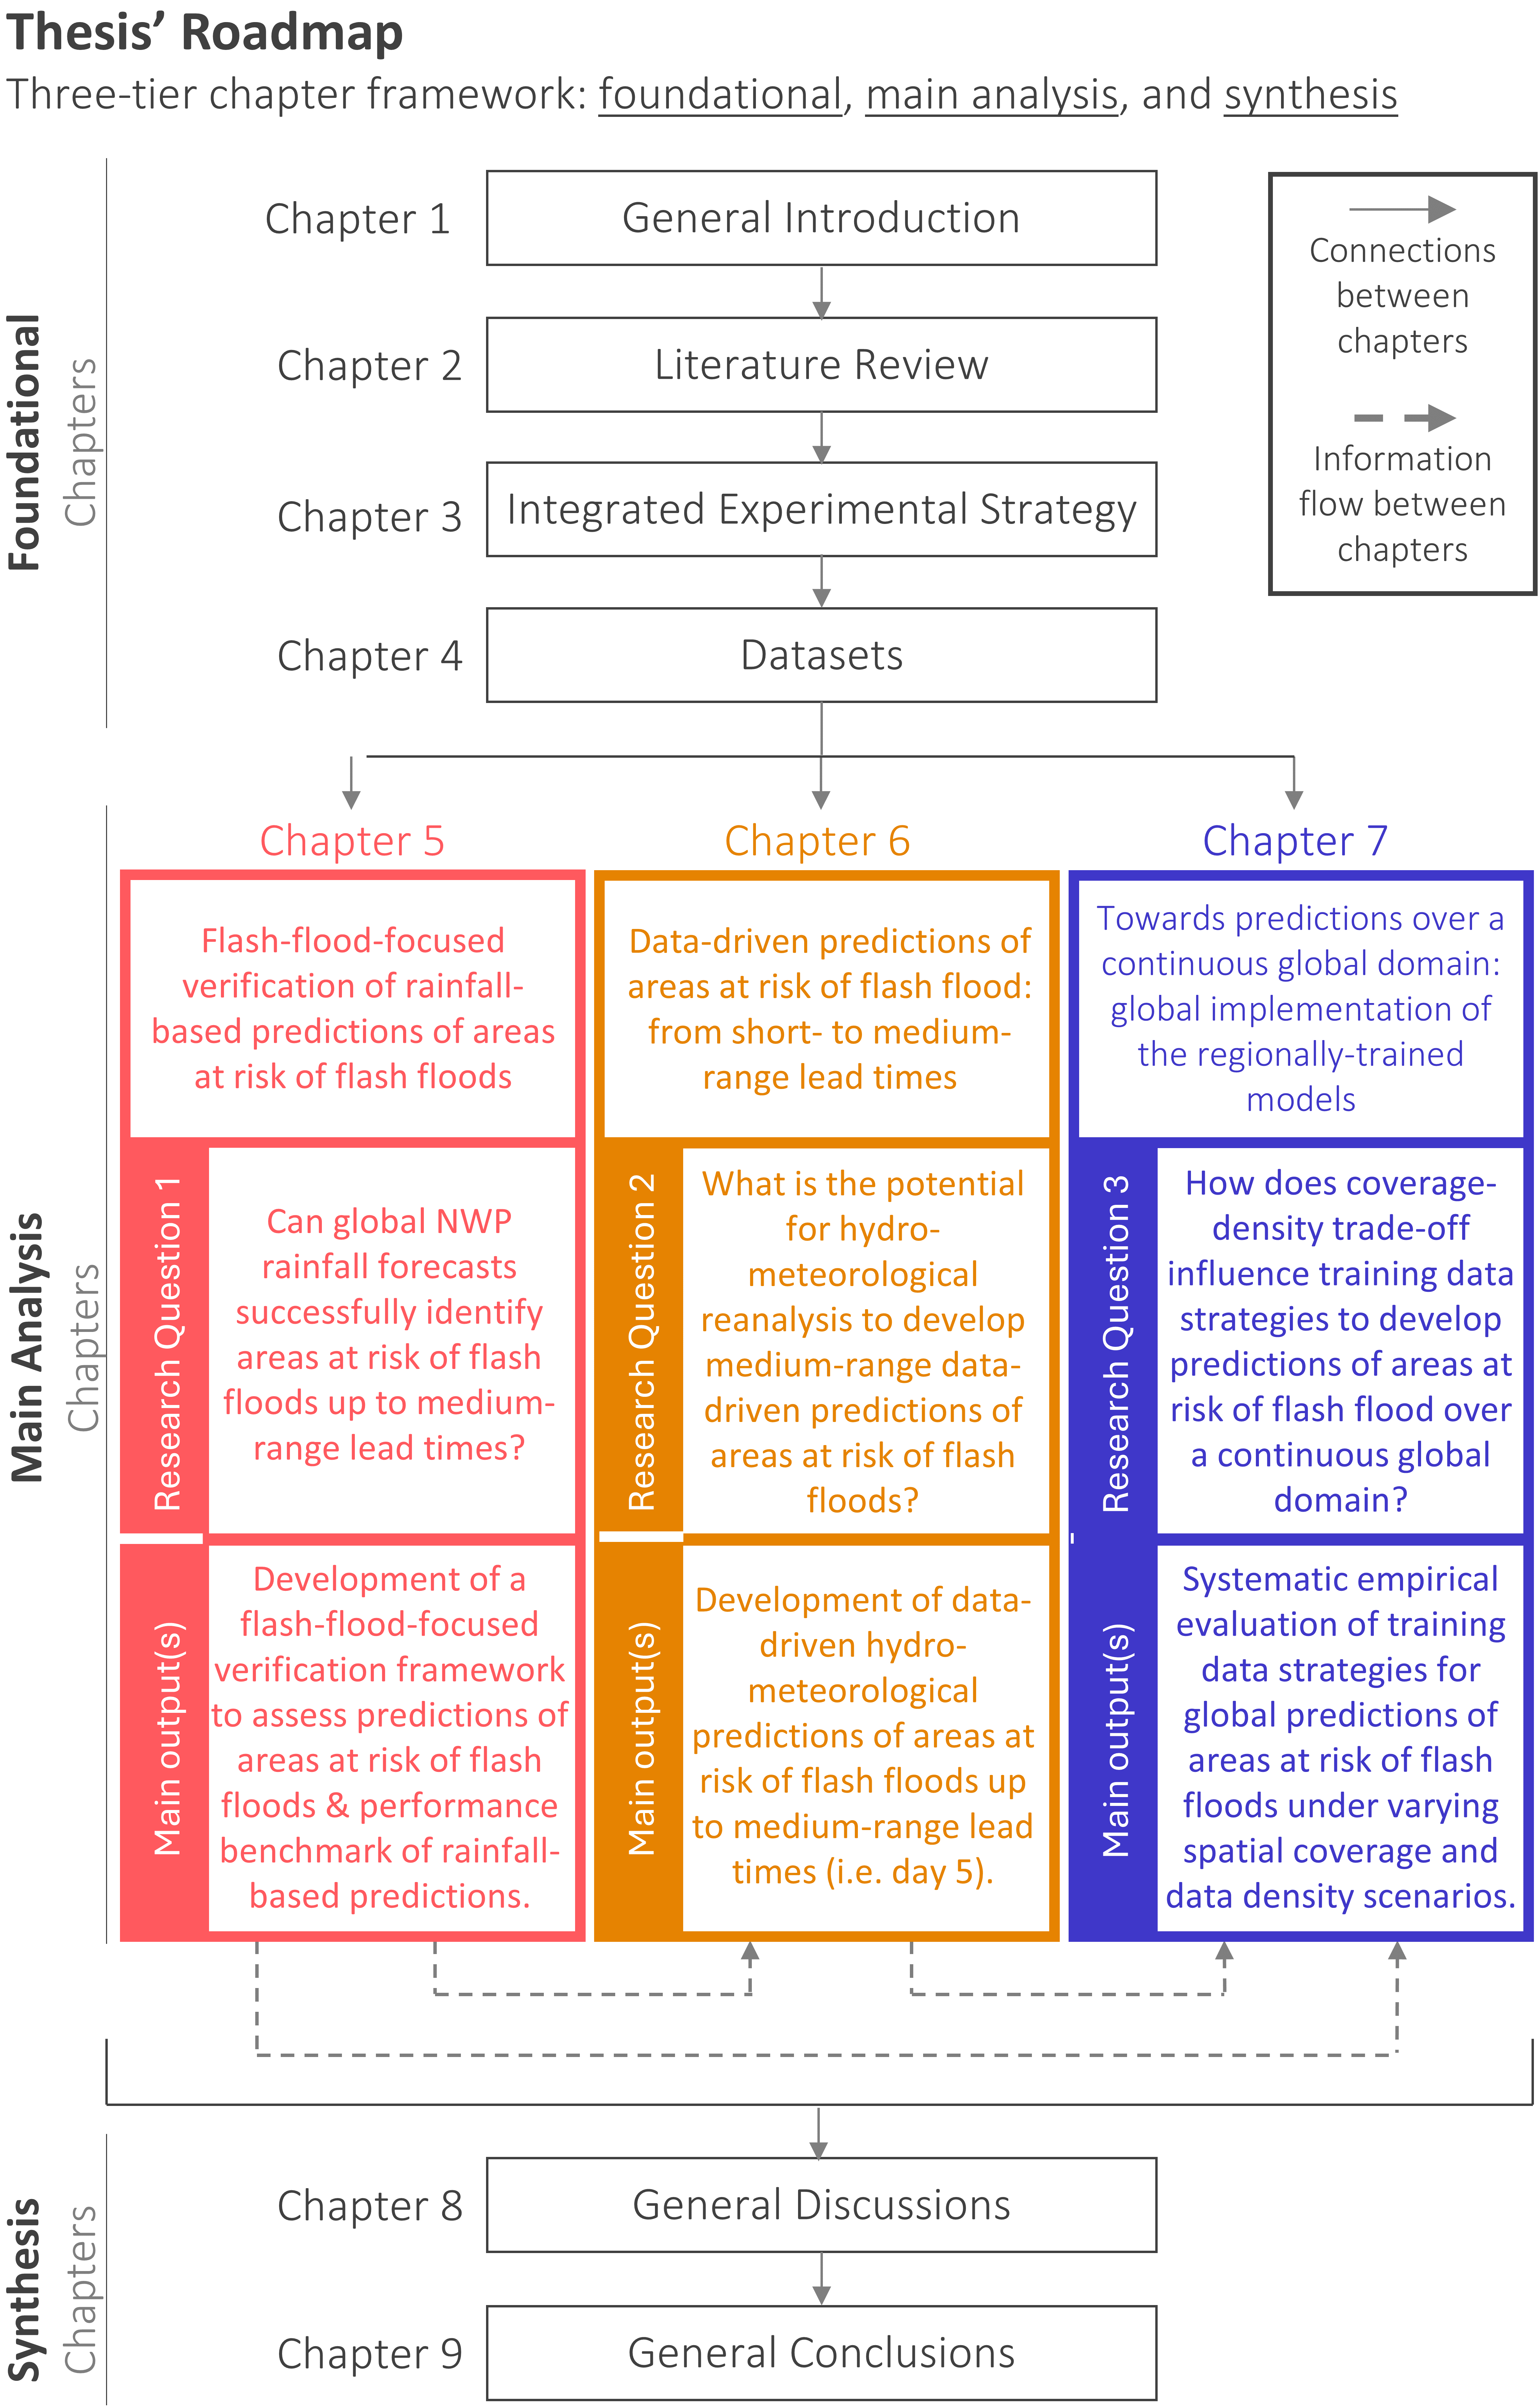
\includegraphics[width=\textwidth]{thesis_roadmap.png}
\caption{\textbf{Thesis roadmap.} It illustrates the progression from the \textit{Foundational Chapters} (General Introduction - Chapter 1; Literature Review - Chapter 2; Experimental Design - Chapter 3; Datasets - Chapter 4), followed by the \textit{Main Analysis Chapters} (Flash-Flood-Focused Rainfall Verification - Chapter 5, indicated in pink; Feasibility of Data-Driven Flash-Flood Prediction Models - Chapter 6, indicated in orange; Predictability of Data-Driven Flash-Flood Forecasts - Chapter 7, indicated in blue), and concluding with the \textit{Synthesis Chapters} (General Discussions - Chapter 9; General Conclusions - Chapter 10).}
\label{fig:thesis_structure}
\end{figure}

\textbf{Chapter 1}\marginpara{Foundational Chapter - General Introduction} established the foundation for this research by addressing the critical need for improved flash flood early warning systems worldwide. The chapter presented the three interconnected research questions addressed in this thesis, i.e., the development of a flash-flood-focused verification framework to assess the performance of global NWP rainfall forecasts in the prediction of areas at risk of flash flood, the creation of data-driven flash flood prediction models using reanalysis data, and the analysis of their predictability up to medium-range lead times. It also introduced the contributions to knowledge and practice in flash flood prediction done by this research that will be further discussed in section \ref{general_discussion_contribution_Knowledge}.

\textbf{Chapter 2}\marginpara{Foundational Chapter - Literature Review} presents a synthesis of the scientific literature in flash flood prediction, establishing the theoretical foundations and delineating the methodological gaps addressed by the three research questions presented in section \ref{general_introduction_research_objectives_questions}.

\textbf{Chapter 3}\marginpara{Foundational Chapter - Experimental Design} delineates the experimental design through which the three research questions are systematically addressed, demonstrating their sequential dependencies and synergistic relationships.

\textbf{Chapter 4}\marginpara{Foundational Chapter - Datasets} presents the datasets considered to address the three presented research questions. It presents the short- and long-range ERA5 rainfall forecasts, post-processed with the ecPoint technique. It also presents the short- and long-range ERA5 forecasts for the soil water content, considered to represent soil's moisture conditions prior the flash flood events. It also presents the climatological parameter characterising the terrain vegetation coverage (i.e., leaf area index), and the static fields representing its steepness (i.e., slope of the sub-grid orography and standard deviation of the filtered sub-grid orography). Moreover, the chapter presents the flash flood impact database used throughout this thesis, NOAA's Storm Event Database, discussing their geographical coverage over the CONUS, its temporal resolution, and its inherent reporting limitations. 

\textbf{Chapter 5}\marginpara{Main Analysis Chapter - Flash-Flood-Focused Rainfall Verification}
introduces a robust flash-flood-focused verification methodology to evaluate the performance of global NWP rainfall forecasts in identifying areas at risk of flash floods, contributing to answering RQ1. The methodology directly verifies rainfall forecasts against flash flood impact observations, addressing challenges such as the interpretation of metrics for dissimilar quantities and managing unreported events. Long-term objective verification and case studies validate the framework while revealing the strengths and limitations of global NWP rainfall forecasts for flash flood prediction. 

\textbf{Chapter 6}\marginpara{Main Analysis Chapter - Feasibility of Data-Driven Flash Flood Prediction Models} examines the feasibility of developing data-driven flash flood prediction models using global ERA5 hydro-meteorological short-range forecasts (up to day 0). The research presents innovative data-driven architectures designed to process ERA5 hydro-meteorological data, carefully considering predictor selection, training strategies, and uncertainty assessment methodologies. Utilising NOAA's Storm Event Database over the contiguous US, the models undergo rigorous validation through both objective score-based verification and subjective case-study analysis following the flash-flood-focused verification framework developed in Chapter 5. The chapter further explores the models' transferability to different geographical regions and climate conditions through sensitivity analyses.

\textbf{Chapter 7}\marginpara{Main Analysis Chapter - Predictability of Data-Driven Flash Flood Forecasts} assesses the predictability of data-driven flash flood forecasts up to medium-range lead times, using ERA5 hydro-meteorological long-range forecasts (from day 1 to day 5), and following the flash-flood-focused verification framework developed in Chapter 5. Building on the data-driven flash flood prediction model developed in Chapter 6, this investigation addresses the challenges of utilising forecast data, including prediction uncertainty and reliability across various lead times through objective verification and case studies. 

\textbf{Chapter 8}\marginpara{Synthesis Chapter - General Discussions} synthesises and discusses the research findings in the main analysis chapters, critically evaluating how effectively each research question was addressed. The chapter explores the broader implications for disaster risk reduction and emergency management, exploring how these advancements may enhance global early warning capabilities against the impacts of flash floods. 

\textbf{Chapter 9}\marginpara{Synthesis Chapter - General Conclusions} concludes the thesis by articulating its novel contributions to flash flood prediction knowledge and practice. It provides final assessments for each research question, acknowledging methodological limitations whilst clearly stating the scientific advancements achieved. The chapter concludes by exploring future research directions that might strengthen the use of forecasts from global NWP models and data-driven approaches for predicting flash floods over a continuous global domain up to medium-range lead times.        % Chapter 1
% %%%%%%%%%%%%%%%%%%%%%%%%%%%%%%%%%%%%%%%%%%%%%%%%%%%%%%
\chapter{Literature review}
\label{literature_review}
\graphicspath{{chapter_02/figures}{chapter_02/tables}}
%%%%%%%%%%%%%%%%%%%%%%%%%%%%%%%%%%%%%%%%%%%%%%%%%%%%%%



\citep{Abegaz_2024} esxample.

This review assesses where the science currently stands to enable the development of a prototype forecasting system that provides medium-range predictions of areas at risk of flash flooding over a continuous global domain. As outlined in Figure \ref{fig:literature_structure}, each thematic section in this chapter is examined through three analytical lenses: \textit{Progress} charts the evolution of knowledge, \textit{Barriers} articulates the limitations that persist or remaining research gaps, and \textit{Opportunities} distils these gaps into the research questions that guide this thesis. By moving systematically from established achievements through current challenges and to future prospects, the chapter positions the reader to understand both the state of the art and the rationale for the analyses presented in the subsequent chapters.

\begin{figure}[htbp]
\centering
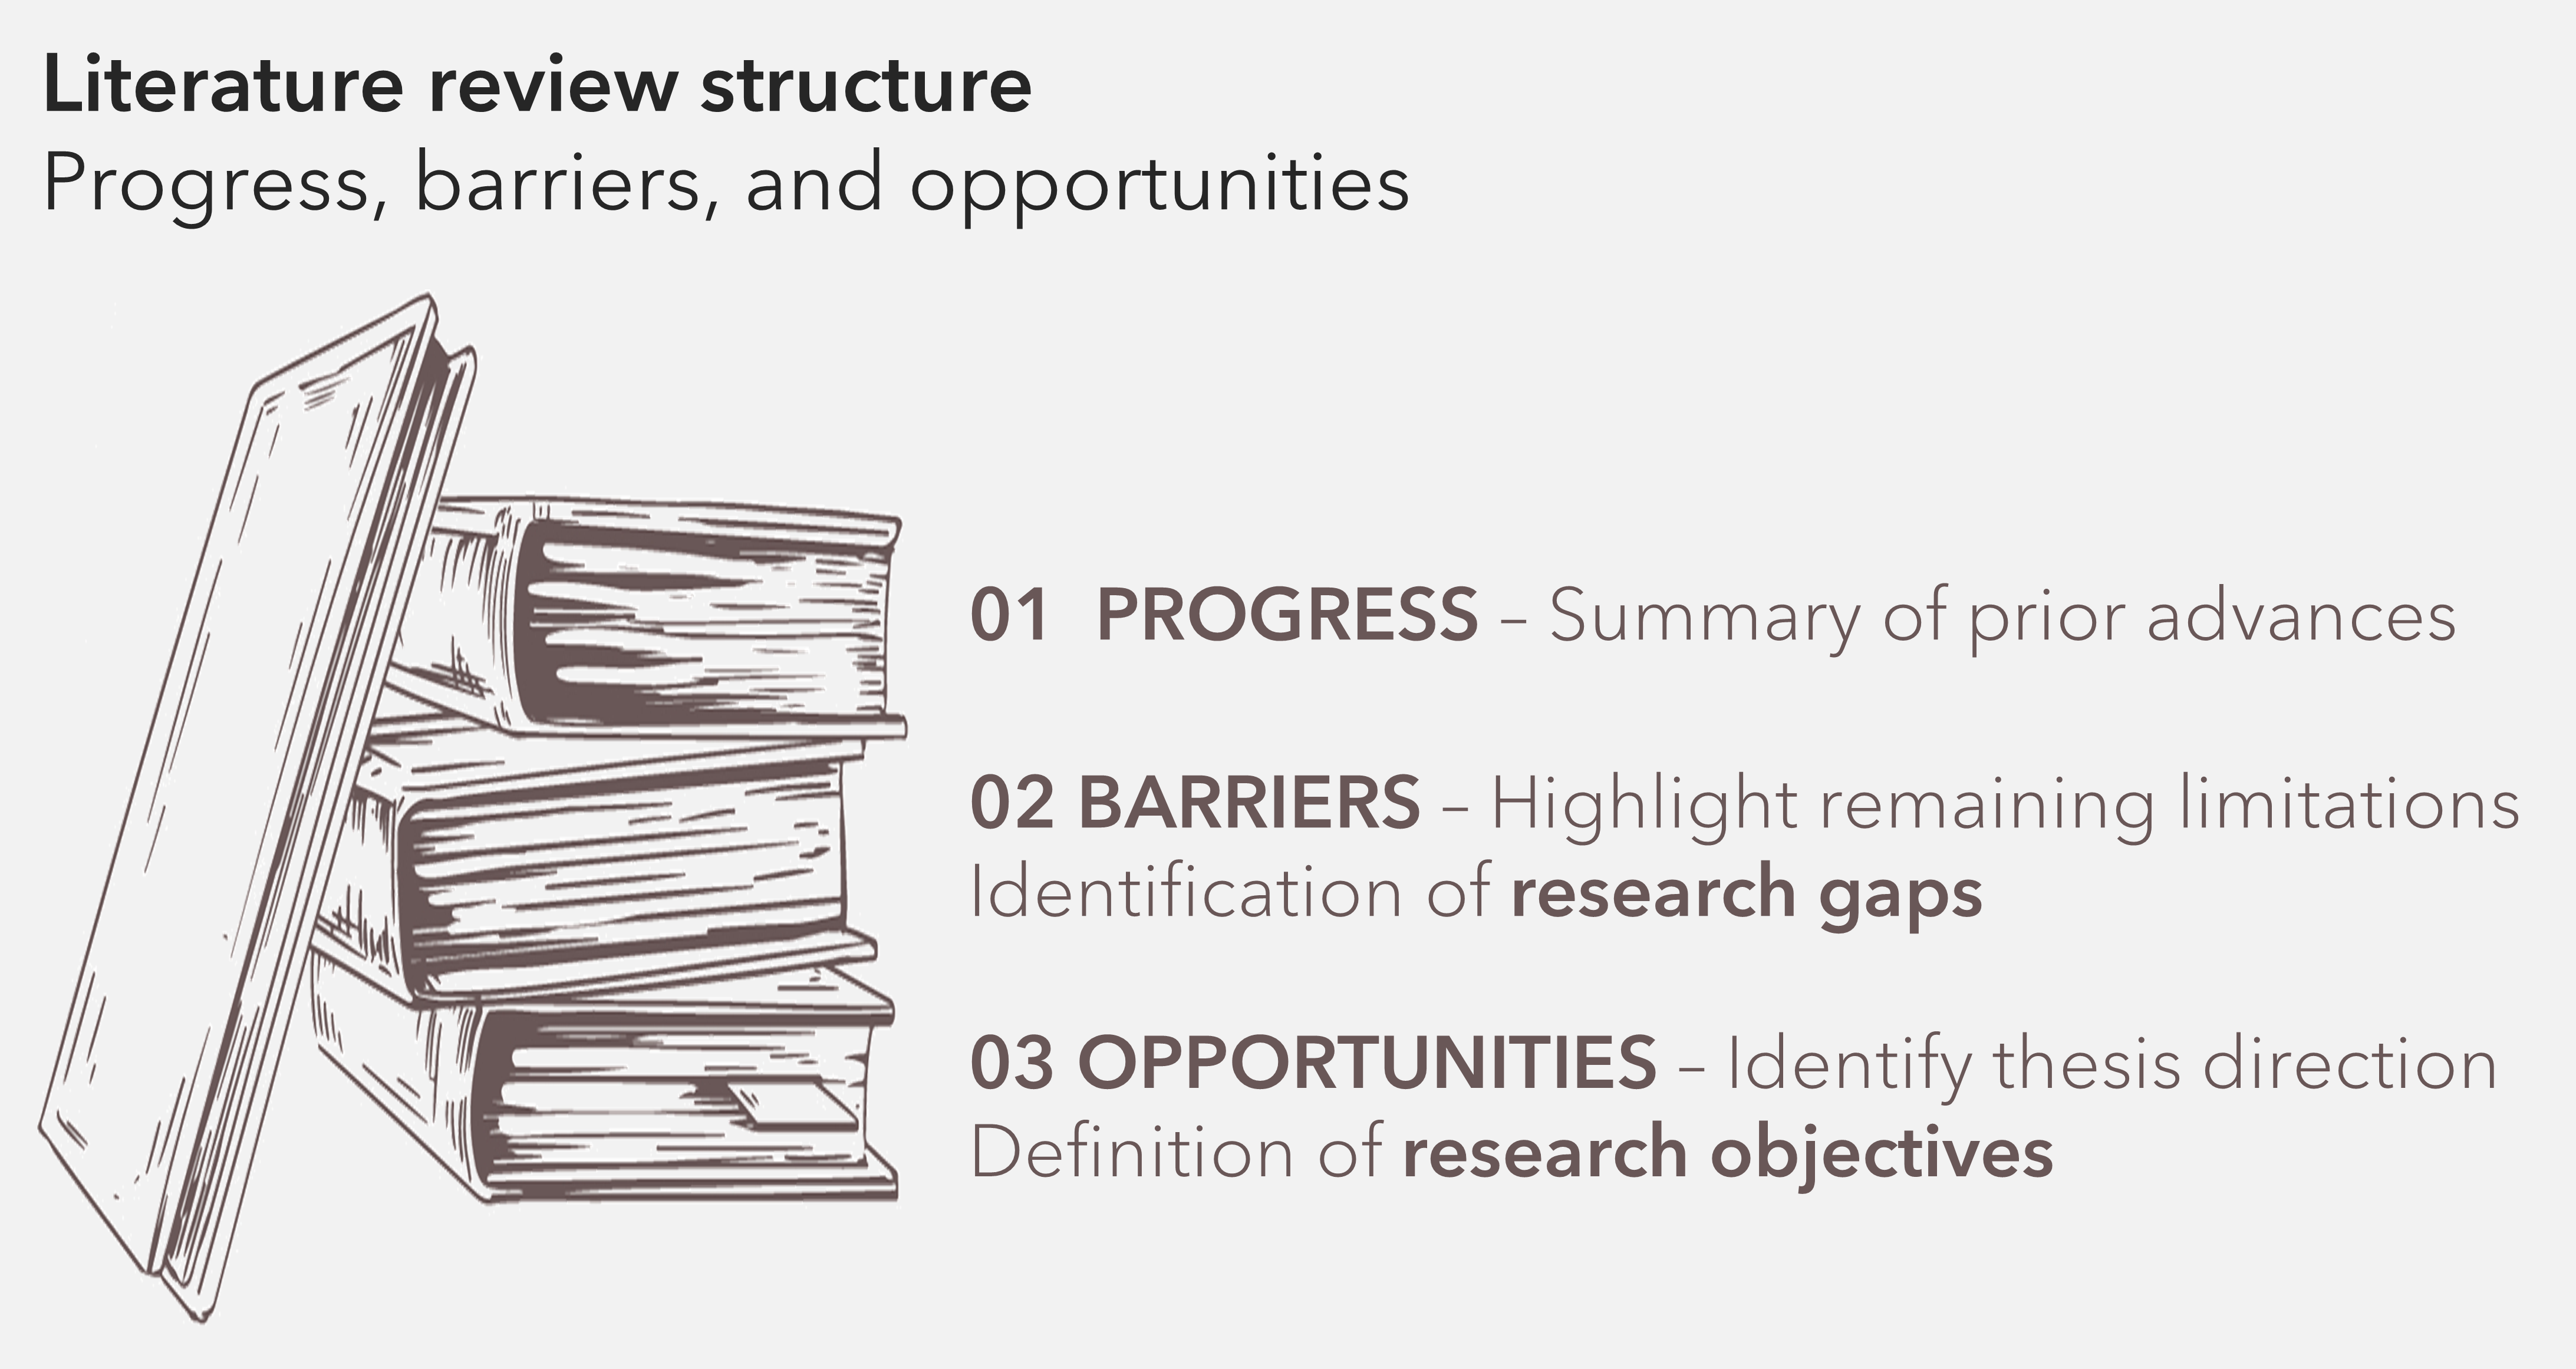
\includegraphics[scale=1.04]{Figures/Chapter_02/literature_structure.png}
\caption{\textbf{Structure of the literature review chapter}.This infographic summarises how each thematic section in the chapter is organised: “\textit{Progress}”, reviews prior work and recent advances, “\textit{Barriers}” delineates the remaining limitations and knowledge gaps, and “\textit{Opportunities}” formulates the research questions pursued in this thesis. Together, these elements guide the reader from established achievements, through current challenges, to future directions that underpin the development of a prototype flash-flood forecasting system providing medium-range forecasts over a continuous global domain.}
\label{fig:literature_structure}
\end{figure}


%%%%%%%%%%%%%%%%%%%%%%%%%%%%%%%%%%%%%%%%%%%%%%%%%%%%%%%%%%%%%%%%%%%%%%%%%%%%
\section{On the use of global NWP rainfall estimates to identify areas at risk of flash flooding}
%%%%%%%%%%%%%%%%%%%%%%%%%%%%%%%%%%%%%%%%%%%%%%%%%%%%%%%%%%%%%%%%%%%%%%%%%%%%

\subsection{Progress}

Flash floods are characterised by a rapid hydrological response to intense rainfall events, with runoff timescales ranging from mere minutes to a few hours \citep{Davis_2001}. While the interaction with local topography, land use, and drainage systems modulates flash flood severity \citep{Marchi_2010, Villacca_2025}, localised extreme rainfall has been shown to be the primary driver of flash floods\footnote{While acknowledging that flash floods can also be triggered by other mechanisms such as ice jams, dam breaks, and landslides, this thesis focuses exclusively on rainfall-triggered flash floods, as they represent the most frequent cause of these events.} \citep{Schumacher_2017, Borga_2014, Archer_2018, Meyer_2022}. Unlike riverine floods that develop gradually over many hours or days from widespread rainfall across large watersheds \citep{Wohl_2022}, flash floods generate in small catchments - typically under 100 $km^2$ or 500 $km^2$ - and within minutes to hours after the triggering rainfall event \citep{Braud_2014, Bloschl_2015}. Hence, accurately characterising and predicting localised extreme rainfall (i.e., its intensity and spatial distribution) determines our ability to identify areas at heightened risk of flash flooding . Near-perfect precision in forecasting the correct distribution of rainfall totals at the precise locations is required, as any underestimation or spatial misplacement, even by a few kilometres, can leave the interested catchment virtually dry and eliminate any flash-flood signal \citep{Nicotina_2008, Douinot_2016, Clark_2016, Wang_2022}.

Several interrelated meteorological factors contribute to extreme rainfall events’ variability in intensity and spatial distribution. The key ingredients of flash flood-producing storms are ample and persistent supply of water vapour, a mechanism to facilitate uplift of air in which the moisture condenses and precipitation forms, and a focusing mechanism (or combination of focusing mechanisms) that causes precipitation to occur continuously or repeatedly over the same area \citep{Doswell_1996}. Large-scale systems such as fronts, cyclones, and troughs can introduce substantial moisture into a region, creating conditions favourable for heavy rainfall. These systems enhance vertical motion and convective activity, leading to localised intense precipitation. Mesoscale convective systems (that is, systems with horizontal scales of 10 to 1000 km) such as squall lines and supercells can dramatically concentrate rainfall over small geographic areas, rapidly overwhelming local hydrological systems \citep{Maddox_1979, Doswell_1996, Davis_2001}. The greatest threat of excessive rainfall and significant flash flooding tends to occur when and where thunderstorms are slow-moving or stationary, continually reform over the same area, or repeatedly move over the same location. For example, if new convection develops on the storm flank opposite the direction of thunderstorm motion, then a quasi-stationary storm complex may evolve. Special circumstances exist in complex terrain where a synoptically forced flow toward and over a topographic barrier may interact with the storm dynamics. This may lead to persistent (slow-moving or quasi-stationary) and orographically enhanced storm systems that produce heavy rainfall through both increased rain rates and increased time raining over a given area Often such precipitation systems are fed by a boundary layer jet (influenced by a stalled frontal boundary) that pumps near-saturated air into the storm, thereby facilitating an efficient formation of precipitation through predominantly warm rain process at relatively low levels in the storm. Regions with an ample supply of moisture from large water bodies, whether seasonally or throughout the year, may exhibit a higher fraction of surface rainfall produced by the warm rain process (as contrasted with the “cold rain” process, which involves evolution from ice particles in the clouds). If this supply of water vapour is combined with orographic uplift (e.g., along Mediterranean coasts of Europe and Northern Africa), this may lead to very effective precipitation production and flash flooding situations.

The correct prediction of such systems remains an ongoing challenge due to the complexity of the atmospheric processes involved. To address these challenges, researchers are developing advanced forecasting tools and early warning systems that integrate high-resolution rainfall observational networks (from rain gauges or radar), km-scale NWP models, and ensemble approaches to quantify uncertainties associated with small-scale weather phenomena and provide more accurate and timely warnings for flash flood events.

For example, many studies show that to obtain better rainfall prediction of localised extreme rainfall events, in terms of location and intensity, the model's resolution must go beyond the "grey-zone" and reach values up to 1 km \citep{Castorina_2022}. These are resolutions that for global models are out of reach for at least a few more decades \citep{Wedi_2020}. Recent developments such as Destination Earth (model at 4.4 km, in the grey zone) confirms these results, as it indeed provides similar skill than the lower-resolution counter part ECMWF's IFS at 9 km. See for example the analysis for the flash floods in Valencia in 2024 \citep{Gascon}.

Flash-flood-producing convective storms have very limited predictability, and forecast skill drops sharply beyond a few hours. Due to the inherent chaotic nature of convection, small initial errors grow quickly, so accurately predicting when and where an extreme downpour will occur more than 6–12 hours in advance is extremely challenging. Indeed, inaccurate rainfall forecasting has been identified as one of the most significant sources of uncertainty in flood prediction \citep{Hapuarachchi_2011}. \citet{Schwartz_2019a, Schwartz_2019b} shows how to increase the forecasts lead times it might be necessary to reduce the members computed and reduce the spatial resolution. 

Despite the advancements produced by Km-scale NWP modelling, there remain different problems when predicting extreme rainfall. 

This motivates the shift toward probabilistic rainfall forecasts. However, even ensemble forecasts struggle with this problem. For short-range forecasts, ensemble forecasts spread can still be large, and important small-scale flash flood-triggering rainfall events may be missed in many members because the scope of the ensemble is to quantify uncertainties in rainfall prediction at its grid scale, ignoring what might be the rainfall at sub-grid scale. 

\begin{figure}[htbp]
\centering
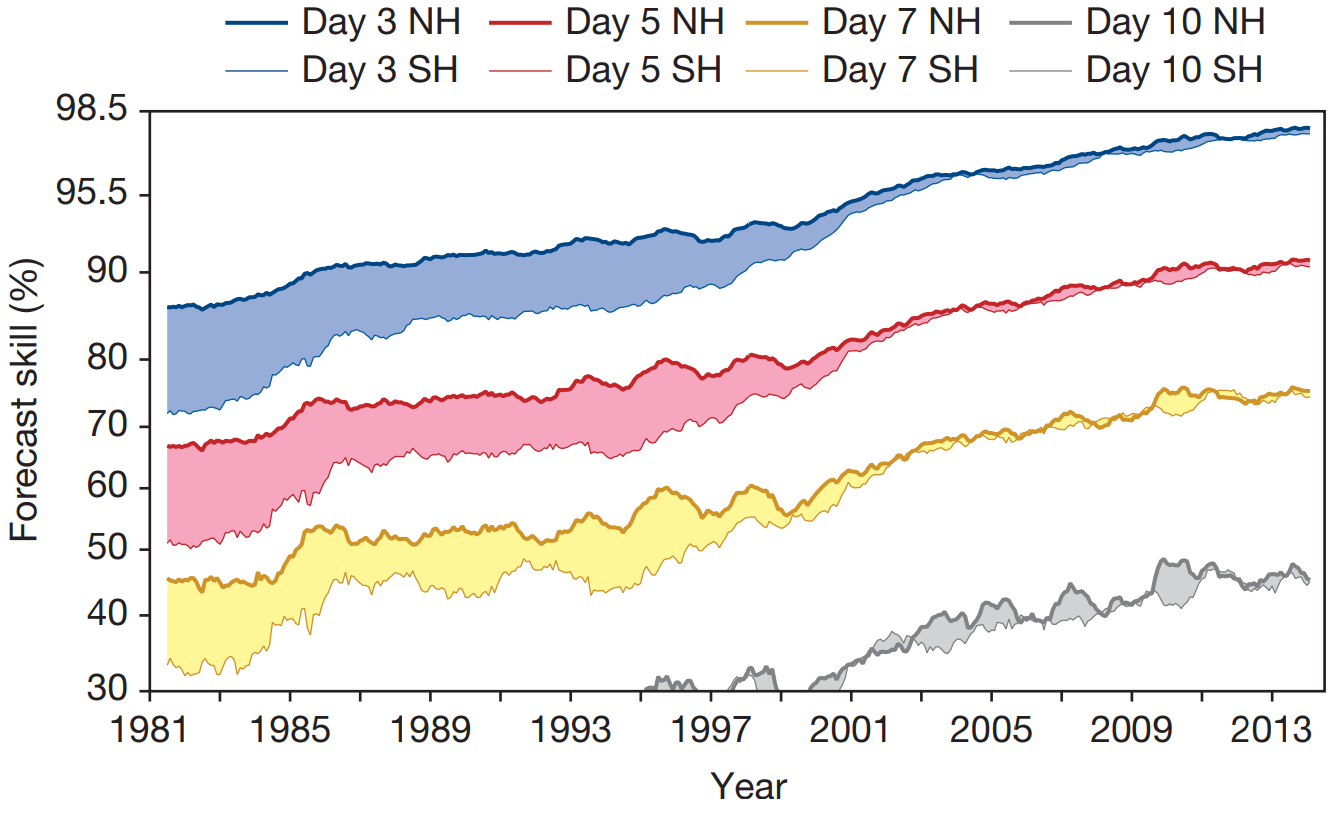
\includegraphics[width=\textwidth]{Figures/Chapter_02/improvement_forecast_skill.png}
\caption{\textbf{Forecast skill improvements for global NWP models, from \citet{Bauer_2015}}. A measure of forecast skill at three-, five-, seven- and ten-day ranges, computed over the extra-tropical northern and southern hemispheres. Forecast skill is the correlation between the forecasts and the verifying analysis of the height of the 500-hPa level, expressed as the anomaly with respect to the climatological height. Values greater than 60\% indicate useful forecasts, while those greater than 80\% represent a high degree of accuracy. The convergence of the curves for Northern Hemisphere (NH) and Southern Hemisphere (SH) after 1999 indicates the breakthrough in exploiting satellite data through the use of variational data.}
\label{fig:improvement_forecast_skill}
\end{figure}

Global NWP models could solve the issues mentioned above. They offer continuous global coverage and produce forecasts up to day 15. Their performance has been increasing steadily, one lead time every decade (Figure \ref{fig:improvement_forecast_skill}). However, for long time they have been considered not appropriate for flash flood prediction due to their coarse resolution (grid-boxes of 10+ km spatial resolution) that cannot explicitly resolve such small-scale intense convection. This often leads to missed or mislocated extreme rainfall totals in the case of small-scale convection \citep{Schumacher_2017}. This barrier is evidenced by cases of “forecast failures” for flash floods due to underestimating localised rainfall intensity, underscoring the need to overcome spatial resolution gaps. 

Notwithstanding, the interest in using rainfall estimates from NWP models has been growing due to their increased performance \citep{Bucherie_2022b}. Moreover, not necessarily coarser NWP models provide rainfall forecasts for extreme rainfall compared to higher-resolution models \citep{Hewson_2024, Wedi_2020}. Furthermore, post-processing offers a great opportunity to post-process medium-range global rainfall forecasts in order to downscale the forecasts and provide rainfall estimates for localised extreme rainfall. One notable example is the post-processing approach called ecPoint, which post-processes global model outputs to provide probabilistic rainfall forecasts at point-scale \citep{Hewson_2021}, and it has been shown to provide forecasts with better skill than raw and post-processed km-scale rainfall forecasts \citep{Gascon_2024}. 

\subsection{Barrier}
Despite the growing interest in considering rainfall estimates from global NWP models to generate forecasts over a continuous global domain and extend predictions to medium-range lead times, there is little verification of such coarser rainfall forecasts for flash flood prediction. The assessment would typically indeed be limited to rainfall observations assuming that if rainfall was correctly predicted, the model would perform equally well if used to predict flash floods \citep{Gascon_2024}. Where comparisons with areas impacted by flash floods, such comparisons are done primarily at local scale \citep{Tripathy_2020}.

While, as stated before, the main driver of flash floods is rainfall, there should be a direct assessment on the capabilities of rainfall forecasts in the prediction of flash flood events. At a local scale, many studies have assessed the capabilities of km-scale rainfall forecasts in the prediction of flash floods. The typical workflow of such studies consists in using the rainfall forecasts to verify as inputs to a hydrological model (with a more or less complex routing process) to compute discharge at a specific location. Such predicted discharge would be compared to observed discharges at the location, and scores routinely used in hydrology such as KGE or NS would be used to assess whether the magnitude of the discharge peak was correct and it was predicted with an acceptable timing. Only \citet{Herman_2018} shows rainfall verification against flash flood reports.  

There are two main problems with this workflow for the verification at a global scale of global NWP rainfall forecasts. The first one is there not exist yet a global hydrological model capable to produce discharge forecasts for small flashy catchments (i.e. below 100 km2) at global scale. Moreover, even if it was possible to create such forecasts the severe paucity of discharge observations in such small flashy catchments (which tend to be ungauged) would prevent any robust verification of such hydrological forecasts, making impossible to assess whether global NWP rainfall forecasts are suitable in identifying areas at risk of flash flooding. Even global discharge databases such as CAMELS or CARAVAN \citep{Kratzert_2023} contain less than 1\% of observations from small-flashy catchments. 

Hence, the assessment of global NWP rainfall forecasts against direct flash flood observations
remains a research gap that impedes the confident use of such forecasts to identify areas at risk of flash flooding.

\subsection{Opportunities}

The recent development of flash flood impact databases at global scale - e.g. EMDAT or Desiventar \citep{cred_2019}, continental scale - e.g., in the US or in Europe \citep{noaa_2019}, and national scale - e.g. in Ecuador  \citep{Bucherie_2022a} have opened up to the possibility of using impact flash flood data as a proxy observation for the identification of areas at risk of flash flooding. They consist in tabular data, in which each data point indicates the location (in the form of latitude/longitude coordinates) and reporting time of a reported flash flood event (including mostly the date but sometimes also the time). If the data points in such databases are pre-processed in a way that indicates in which grid-boxes flash flood events were observed (binary yes- or no-events), they could be used to run a first assessment on whether the global NWP rainfall forecasts identify the grid-boxes where the flash flood events were observed.

While it would not be possible to assess the timing, location, and magnitude of the flash flood event with score commonly used in hydrology because the rainfall is not transformed in discharge, and discharge observations are not considered, it would be possible to at least assess whether the rainfall forecasts are able to provide guidance on what are the grid-boxes likely to experience flash flooding adopting commonly used scores in probabilistic verification such as reliability diagrams, frequency bias, and roc curves. While this verification provides an outlook of flash flooding conditions, this information is useful to understand whether the rainfall forecasts contain any information regarding potential flash flooding \citep{Mason_1979}, and hence it is worth pursuing more complex hydrological modelling with such rainfall forecasts as input. 

Two aspects must be considered when implementing any verification framework using impact flash flood reports. First, this type of observations are not static like measurements coming from rain or discharge gauges, which report yes- \textit{and} no-events. With the latter is indeed possible to assess whether the model produces a correct prediction (in the case the event was or not predicted, and the event did or did not happened) or a wrong prediction (in the case the event was or not predicted, and the event did not or did happened). Impact databases include only events that \textit{were} reporter, and it is not known whether a no-report represents an event that happened but it was not reported or it represents an event that did not happen. This uncertainty makes difficult to assess whether an event was correct to not. Moreover, we do know that impact databases severely underestimate the frequency of flash flood occurrence \citep{Panwar_2020}. Hence, it is likely that any verification would overestimate the cases in which correct forecasts might be considered as wrong, undermining the assessment of the forecasts and their potential usability in the prediction of areas at risk of flash flooding. 

Despite these difficulties and including appropriate considerations around uncertainties surrounding the observational dataset, it is expected that the verification of rainfall forecast against impact flash flood reports will shed light on the capabilities of global NWP models in identifying areas at risk of flash floods. 

The research developed around this topic will be presented in chapter 5. 


%%%%%%%%%%%%%%%%%%%%%%%%%%%%%%%%%%%%%%%%%%%%%%%%%%%%%%%%%%%%%%%%%%%%%%%%%%%%
\section{On the use of reanalysis data and machine learning to create a prototype forecasting system that provides short-range predictions of areas at risk of flash flooding over a continuous global domain}
%%%%%%%%%%%%%%%%%%%%%%%%%%%%%%%%%%%%%%%%%%%%%%%%%%%%%%%%%%%%%%%%%%%%%%%%%%%%

\subsection{Progress}

In the previous section we have highlighted how important is to have rainfall forecasts that correctly locate the extreme rainfall in order to identify areas a t risk of flash flood. In this section, it will be discussed how catchment characteristics play a crucial role in determining the hydrological response to flash flood events, and how hydrologists have tried to model those interactions in order to produce flash flood predictions. 

Catchment characteristics play a crucial role in determining the hydrological response to flash flood events. The morphology, topography, land use, and soil properties of a catchment substantially influence its behaviour during extreme rainfall \citep{Henao2022, Liu2011}. Key factors such as antecedent moisture conditions, soil type, and vegetation cover are essential for evaluating runoff generation \citep{Henao2022a, Liu2011}. The scale and size of catchments add complexity to hydrological responses, with larger catchments exhibiting greater heterogeneity in their hydrodynamic behaviours \citep{Luong2021}. Catchment topography significantly modifies water movement patterns, with steeper slopes promoting quicker runoff travel times and concentrated flow pathways \citep{Liu2011, Maqtan2022a}. Soil moisture and infiltration rates are critical hydrological factors governing the occurrence and intensity of flash floods. Initial soil moisture conditions directly influence runoff generation through their effect on infiltration capacities and connectivity between surface and subsurface flow pathways \citep{Yatheendradas2008}. Flash flood forecasting systems rely heavily on accurate initial soil moisture estimates to simulate hydrological responses effectively \citep{Yatheendradas2008, AlRawas2024, Xing2019a}. Uncertainty in initial soil moisture assessments remains a challenge due to spatial heterogeneity and temporal variability in environmental factors \citep{Yatheendradas2008, AlRawas2024}. Streamflow dynamics constitute a critical aspect of hydrological factors influencing flash flood behaviour, encapsulating interactions between surface water flow and driving meteorological inputs \citep{Yang2022}. Spatial variability plays an instrumental role in shaping streamflow characteristics, with the heterogeneity of river basins affecting how water converges and accelerates in channels \citep{Zhang2024}. Accurate measurement of streamflow dynamics hinges on advancements in real-time monitoring technologies and the integration of varying data types into computationally demanding hydraulic simulations \citep{Msigwa2024, Barthold2015}.

Flash flood forecasting has evolved dramatically over the decades, transforming from basic hydrological calculations to sophisticated AI-powered prediction systems that save countless lives worldwide.

The foundations of flash flood forecasting were established through fundamental hydrological concepts developed in the mid-20th century. The unit hydrograph principle became a cornerstone concept for understanding how rainfall translates into streamflow in small watersheds \citep{Rigon2016}. These early approaches relied primarily on mathematical representations of watershed behaviour, with limited data collection capabilities and processing power. Early forecasting methods depended heavily on ground-based observations using in situ sensors, which provided relatively limited spatial coverage and temporal resolution \citep{Tao2024}. During this period, hydrologists developed theoretical frameworks that enabled more sophisticated forecasting. Concepts like lag time, storage, and the geomorphological unit hydrograph emerged as critical tools for understanding the timing and magnitude of flood responses \citep{Rigon2016}. These approaches were mostly applied to larger river systems with longer response times, leaving flash flood prediction, characterised by rapid onset and localised impacts, as a particularly challenging problem for forecasters. 

The late 20th century saw increasing efforts to translate theoretical hydrological understanding into operational forecasting systems for flash floods. This period was characterised by growing recognition of flash floods as a distinct hydrological hazard from the other types of floods, requiring specialised prediction approaches. Early warning systems during this era were primarily deterministic, using rainfall observations and simple rainfall-runoff models to predict potential flooding \citep{Hapuarachchi2011}. As computational capabilities improved in the 1980s and 1990s, more sophisticated hydrological models began to emerge, like the flash flood guidance system in the US \citep{Georgakakos_1986}. However, these early systems were limited by data availability, computational constraints, and a lack of integration between meteorological and hydrological forecasting components. Despite these limitations, they represented important steps toward developing dedicated flash flood prediction capabilities as they form the foundation of the more modern system in the 21st century. 

The beginning of the 21st century marked a pivotal moment in flash flood forecasting. A key innovation in modern flash flood forecasting systems has been their ability to integrate diverse data sources. These systems incorporate remotely-sensed precipitation data from geostationary and polar orbiter satellite platforms, reflectivity data from weather radar systems, and ground-based automated precipitation gauge measurements. This multi-source approach helped overcome the limitations of any single data type and provided more robust precipitation estimates, which are the most critical input for flood forecasting. The systems also evolved to include mesoscale NWP model forecasts integrated with land-surface model responses, enabling the creation of forecast products with longer lead times, i.e. up to 24h rather than a few hours. This integration of atmospheric and hydrologic modelling represented a significant advance over earlier, more compartmentalised approaches to flash flood prediction. The technological revolution has also played an important role in developing operational flash flood forecasting systems. As computational demands for flood forecasting increase, high-performance computing clusters become essential infrastructure for operational systems. For example, a parallel flood forecasting and warning platform, based on high-performance computing clusters, was established in China, enabling nationwide coverage with particular effectiveness for flash flood prediction. This platform utilises advanced file-based message passing on a shared hierarchical storage system, pre-allocation and dynamic allocation methods for resource management, and automatic switching between different time-scale models driven by rainfall events. These computational advances allowed for unprecedented spatial and temporal resolution in modelling, enabling more localised and accurate predictions. The ability to process vast quantities of data in near-real-time transformed the capabilities of forecasting systems, substantially reducing the gap between observation and warning issuance.

Despite the technological advances, these systems were developed for small-scale domains, such as urban, regional, or national. Urban flash flood forecasting requires specialised approaches due to complex city environments with varied land use, impermeable surfaces, and intricate drainage systems. Traditional channel models often fail to capture localised ponding scenarios independent of river overflow. Challenges include predicting pluvial flash floods, where rainfall directly generates surface runoff without channel interaction, and insufficient integration of socioeconomic vulnerability data. Innovations include high-resolution DEMs, real-time IoT sensor networks, machine learning algorithms, and ensemble precipitation modelling. Future systems must integrate hydrological observations with meteorological forecasts and regional thresholds to improve prediction accuracy in expanding urban landscapes. Regional and national forecasting systems enhanced localised flash flood prediction capabilities. These systems are designed to address their host countries or regions' specific geographic, climatic, and infrastructural conditions. By leveraging lower-resolution data inputs (e.g. from national-scale NWP models) and incorporating locally sourced datasets, they refine predictions and improve actionable outputs. The Cascading Forecasting Process, utilised within frameworks such as the Southern Africa Severe Weather Forecast Demonstration Project (SWFDP), exemplifies this approach. It facilitates the transfer of forecast outputs from advanced global centres to designated regional hubs, which interpret and provide guidance on imminent severe weather events \citep{Jubach2016}. Effective regional systems rely heavily on local ownership and accessibility of input data, often maintained under specific agreements by hydro-meteorological agencies or related institutions. This underscores the importance of robust inter-institutional collaboration \citep{Georgakakos2022}. Despite advancements in spatial resolution, adaptability, and probabilistic approaches \citep{Zanchetta2020, AlRawas2024}, challenges persist in less monitored areas where gauging stations are sparse \citep{Kuksina2020}. Addressing these observational gaps while maintaining fidelity across models tailored to specific catchments is crucial for system resilience due to climatic variability and infrastructure limitations \citep{Liu2011, Douinot2016}. 

While the theoretical and technological advances in the prediction of flash floods was important, it was still not possible to extend such complex systems at larger domains such as continental or global scale. 

From the 2010s, prototypes for continental flash flood forecasting systems started to emerged. These systems process vast amounts of global meteorological data to provide scalable predictions that can be tailored to specific regions or localised events. Operational frameworks have been established to incorporate global-to-regional interlinkages, facilitating effective information dissemination for disaster prevention initiatives at multiple scales \citep{Georgakakos2022}. However, these systems face challenges in integrating heterogeneous factors that influence flash floods, such as precipitation variability across large geographical extents and interconnected physical processes like soil permeability and lithological characteristics \citep{Henao2022, Henao2022a, Kuksina2020}. Addressing uncertainties associated with model implementations for predicting localised extreme rainfall occurrences is another fundamental consideration. Misalignments between simulated precipitation outputs and real-time weather anomalies become more pronounced at broader spatial scales \citep{Maqtan2022a, Maqtan2022b}. Continental-level systems often employ probabilistic frameworks enhanced by multi-source satellite measurement tools, such as the Integrated Multi-Satellite Retrievals for Global Precipitation Measurement (IMERG). Coupling these with emergency planning modules targeting exposure minimisation during high-risk intervals is a hallmark application that leverages global coverage advantages and computational advancements \citep{AlRawas2024}.

Such continental prototypes needed data-rich implementations. Hence, they were developed mainly in data-rich continents like the US and Europe, leaving many regions, especially in the Global South, under-covered or not protected at all. 

Physical models are a critical component of flash flood forecasting systems, employing principles derived from physical laws and equations to simulate hydrological processes. These models capture the intrinsic behaviour of natural processes such as precipitation-runoff transformations, soil infiltration, and river routing without relying on statistical or empirical relationships \citep{Hinge2024}. Operational systems like the Ensemble Framework For Flash Flood Forecasting (EF5) incorporate physical models to produce actionable runoff predictions while maintaining computational feasibility \citep{Flamig2020}, and their scalability allows for iterative improvements and parameter adjustments across diverse spatial domains \citep{Xing2019a}. Physical modelling intersects with uncertainty quantification frameworks, such as ensemble-based methods or probabilistic estimations, and systems like Flood-PROOFS utilise downscaling techniques to refine deterministic weather predictions into high-resolution forecasts for flash flood risk evaluation \citep{Zanchetta2020}. Challenges persist in achieving universality due to varying regional requirements and climatic patterns \citep{Xing2019a, AlRawas2024}. However, application frameworks like FLASH leverage ensemble configurations and physically-derived parameters to assimilate real-time meteorological inputs accurately, improving lead times for emergency alerts \citep{Martinaitis2023}. 

Data-driven models have gained prominence in flash flood forecasting due to their ability to leverage large datasets and identify complex patterns in meteorological and hydrological variables. These models employ statistical, machine learning, or neural network techniques to predict flash flood occurrences and associated risks based on historical and real-time data. A notable example is the Data-Driven Hydrological Model (DaHM), which uses a feed-forward two-layer perceptron architecture to capture non-linear relationships between input variables like precipitation and streamflow \citep{Philipp2016}. Data-driven frameworks offer the advantage of relying on empirical data rather than explicitly defined physical equations, enabling a broader range of applications where observational data is abundant \citep{Zanchetta2020, Msigwa2024}. However, their robustness is tied to the availability and quality of input datasets, and challenges arise in regions with limited historical records or sparse monitoring networks \citep{Zanchetta2020, Lu2021}. Despite inherent uncertainties in predicting localised extreme rainfall events, data-driven models continue to evolve by combining traditional observational techniques with machine learning components \citep{AlRawas2024}. Coupling data-driven models with physics-based frameworks leverages the strengths of both paradigms, fostering improvements in predictive skill and actionable knowledge dissemination \citep{Msigwa2024}. 

\subsection{Barriers}

As emerging models develop under expanding computational power and integrated datasets, there remain significant research gaps for the development of a flash flood forecasting system over a co ntinuous global domain. 

Data-driven approaches are increasingly being explored for flash flood forecasting, with the aim of overcoming limitations of traditional physics-based methods in data-sparse regions, as stated in the previous section. Recent reviews indicate that a majority of flash flood prediction studies now incorporate machine learning or artificial intelligence techniques \citep{AlRawas2024}, reflecting a shift toward data-driven modelling. Key considerations include the selection of predictive features, the scarcity and quality of historical flash flood observations, suitable forecasts, suitable model architectures, uncertainty quantification, and the computational trade-offs inherent in operationalising such a system.

A fundamental hurdle in developing data-driven flash flood models is the scarcity of reliable historical event data for model training and validation. Flash floods are relatively infrequent and highly localised, and unlike river floods, they often occur in ungauged basins with no stream gauge records of discharge or water level. Many flash flood events are documented only anecdotally (e.g., through post-event reports, disaster databases or news media) or via indirect observations (damage reports, remote sensing of flood aftermath). This leads to a paucity of labelled examples for supervised learning. The limited sample of flash flood occurrences also introduces a strong class imbalance: most time steps and locations correspond to “no flash flood” conditions, which can bias a model unless special training strategies are adopted. Some regions have assembled flash flood event catalogues — for instance, the U.S. and Europe maintain databases of flash flood reports — but globally, there is no unified flash flood archive with consistent reporting criteria. Modellers must therefore integrate heterogeneous data sources or use proxies to identify flash flood events in historical records. One feasible approach is to leverage reanalysis-driven hydrological simulations as a substitute for direct observations of flash flooding. \citet{Alkaabi2025} demonstrate this strategy in a data-sparse desert catchment: they first validated ERA5-derived runoff against a calibrated hydrologic model (HEC-HMS) for past storm events, then used the reanalysis precipitation-runoff pairs to train a deep learning model for flash flood runoff prediction. By doing so, they generated a training dataset from reanalysis that mimics the catchment’s flood response without extensive gauged flow data. Another example is the use of global runoff models or flood reanalysis products (e.g., GloFAS reanalysis) to identify periods of extreme flow that correspond to flash flooding conditions \citep{Wu2022}. While these proxies are imperfect – hydrologic models have their uncertainties – they can considerably expand the training sample size. Additionally, remote sensing offers emerging means to detect flash flood impacts (e.g., sudden increases in river turbidity or soil wetness observable by satellites), which could infer flash flood occurrences in ungauged basins for model training \citep{Smith2021}. Despite such innovations, the challenge of limited ground truth data remains a central issue for global flash flood prediction feasibility. It is difficult to capture the full spectrum of flash flood phenomena (from minor inundations to catastrophic torrents) with coarse datasets. Many events, especially in remote regions, may go unrecorded, leading to under-reporting bias. Models trained only on recorded events might struggle to predict floods in regions with no history in the dataset, even if physical conditions are ripe for flooding. Data augmentation and transfer learning become important in this context: by training on diverse climates and geographies, a model may learn general patterns that transfer to ungauged locations. Recent work in hydrology has shown that deep learning models can indeed extrapolate to ungauged basins by exploiting large training samples and catchment descriptors \citep{Kratzert2019, Gilon2024}. However, those efforts have primarily addressed riverine floods; flash floods pose additional complexity due to their rapid onset and small spatial scale. In summary, assembling a representative and extensive training dataset for global flash flood prediction is non-trivial. It likely requires combining multiple data sources (reanalysis, remote sensing, simulated events, and whatever observational records exist) to capture both positive cases (flash flood occurrences) and negatives (similar meteorological events that did not cause flooding). Careful curation of such a dataset is critical to the feasibility of any data-driven flash flood model. 

\section{Opportunities}

Applications of AI in problems with similar issues to those presented so far, i.e. severe imbalanced datasets in the prediction of lightning \citep{Cavaiola_2024} have shown the benefits of adopting machine learning algorithms to predict flash flood events. 



%%%%%%%%%%%%%%%%%%%%%%%%%%%%%%%%%%%%%%%%%%%%%%%%%%%%%%%%%%%%%%%%%%%%%%%%%%%%
\section{On the use of medium-range NWP forecasts and machine learning to assess the predictability of predictions of areas at risk of flash flooding over a continuous global domain up to medium-range lead times}
%%%%%%%%%%%%%%%%%%%%%%%%%%%%%%%%%%%%%%%%%%%%%%%%%%%%%%%%%%%%%%%%%%%%%%%%%%%%

\section{Progress}
Medium-range prediction, defined as forecasts up to 10 days ahead, has historically been elusive due to the complex, localised nature of the flash-flood-triggering rainfall events and the hydrological processes that generate the flash flood events themselves. 

Prior to the 2000s, flash flood forecasting was largely limited to very short lead times (hours to 1-2 days) due to limitations in numerical weather prediction (NWP) models and computing power. The foundations began in the 1970s with basic hydrological models and limited meteorological forecasting capabilities, exemplified by the establishment of the U.S. National Weather Service Flash Flood Program \citep{Georgakakos_1987}.

A significant shift occurred in the early 2000s, particularly after devastating floods in Europe. The development of the European Flood Alert System (EFAS) in 2003 represented one of the first major attempts at medium-range flood forecasting. This era marked the critical transition from deterministic to probabilistic forecasting approaches—a fundamental requirement for extending prediction lead times beyond 3 days. By 2020, systems like EFAS Version 4.0 introduced sub-daily calibration of hydrological models, significantly improving medium-range forecast accuracy for medium- to large-scale catchments \citep{Mazzetti_2021}. This allowed to represent medium-scale flash flood events (i.e. those where hydrological and routing processes are important), while small-scale flash floods events (i.e. primarily dependent on extreme localised rainfall events) remained largely underrepresented. At global scale, GLOFAS remain out of scope for the representation of global small- and medium-scale flash flood events. 

Several key technological breakthroughs enabled this extension from short-term to medium-range flash flood prediction: (1) ensemble prediction systems that quantify forecast uncertainty \citep{Martinaitis_2023, Flamig_2020}, (2) high-performance computing allowing more sophisticated modelling, (3) improved precipitation measurement through multi-satellite products and dual-polarization radar, (4) evolution of distributed hydrological models, and (5) the integration of machine learning and artificial intelligence techniques.


\section{Barriers}

Despite significant advances, medium-range flash flood prediction faces substantial challenges globally. While the use of medium-range global NWP models have been used since the 2000s to extend to medium-range lead time the hydrological predictions for large-scale hydrology \citep{Gouweleeuw_2005}, the primary limitation of extending hydrological predictions at all scales remains precipitation forecast uncertainty at the 5-10 day range \citep{Jasper_2002}. Hence, the cascade of uncertainty from precipitation forecasts through hydrological models continues to constrain prediction skill \citep{Georgakakos_2022a}. 

Flash floods result from convective storms that are notoriously difficult to predict beyond 1-2 days due to spatial and temporal resolution limitations of global NWP models, which typically operate at resolutions too coarse (10-25 km) to resolve the small-scale processes that trigger flash floods. However, at least at regional scale, it has been shown against flash flood impact observations that if the rainfall forecasts contain some useful guidance on the occurrence of extreme rainfall events, it is reasonable to assume that reasonable performance can be achieved at predicting areas at risk of flash floods even up to day 15 \citep{Tripathy_2020}.

Moreover, we are faced with the challenge to predict so-called "unprecedented events", events that are not present in our observational records, and people are not prepared for as shown by deadly rainfall-triggered flash floods and landslides causing hundreds of deaths and economic losses \citep{Marengo_2023, Marengo_2024, Alcantara_2023}. Future projections indeed state that we need to prepare for worse flash flood events in the near future \citep{AlRawas_2024a}.

While applied primarily for large catchments, studies show that to enhance the predictability of flood predictions, it is necessary to also quantify the uncertainty in the hydrological models to provide skillful forecasts up to day 10 \citep{Teja_2023}. However, for flash floods even the most recent developments such as EF5 \citep{Flamig_2020} provide forecasts up to 24 hours ahead, including the latest developments that use data-driven approaches \citep{Nevo_2022, Nearing_2024}. 

Hydrological model challenges include parameter uncertainty (especially for ungauged catchments), dependency on accurate initial soil moisture conditions, and scale mismatches between model resolution and the small catchments where flash floods typically occur. The combination of meteorological and hydrological uncertainties creates a cascade effect, with errors in precipitation forecasts amplifying when propagated through hydrological models. 

Regional disparities in observation networks create significant limitations for the development of a flash flood forecasting system over a continuous global domain up to medium-range lead times . While North America, Europe, and parts of East Asia benefit from dense networks of weather radars and gauges, many parts of Africa, South Asia, and South America lack adequate ground-based observation networks, particularly in mountainous areas where flash floods frequently occur. 

\section{Opportunities}

Addressing these challenges will require continued investment in high-resolution modelling, ensemble prediction systems, improved data assimilation, and machine learning techniques adapted to the specific conditions of each region, data-driven approaches could help us to make steps forward in the creation of medium-range flash flood forecasting system over a continuous global domain.

The future of medium-range flash flood prediction lies in hybrid approaches that leverage both physical understanding and data-driven insights, enhanced observational networks including non-traditional data sources, and impact-based warning frameworks that translate flood forecasts into actionable information for vulnerable communities worldwide. 

\citep{Cavaiola_2024} shows the benefits of adopting data-driven approaches in the prediction of lightning (a problem showing similar issues with imbalanced datasets) up to medium-range forecasts (although here medium-range is considered only up to t+48). 
       % Chapter 2
%%%%%%%%%%%%%%%%%%%%%%%%%%%%%%%%%%%%%%%%%%%%%%%%%%%%%%
\chapter{Experimental design}
\label{experimental_design}
\graphicspath{{chapter_03/figures}{chapter_03/tables}}
%%%%%%%%%%%%%%%%%%%%%%%%%%%%%%%%%%%%%%%%%%%%%%%%%%%%%%


This chapter articulates the sequential experimental strategy designed to address the research questions presented in Chapter \ref{general_introduction} and provide the proof of concept for medium-range predictions of areas at risk of flash floods across a continuous global domain. The strategy follows a three-component approach, where each component builds upon the findings of the previous one (Figure \ref{fig:workflow_dataflow}). 

The \marginpara{First methodological component (addressing RQ1): development of a flash-flood-focused verification framework to assess predictions of areas at risk of flash flood} first methodological component addresses the challenge that high-quality rainfall forecasts do not necessarily translate directly to accurate flash flood predictions. It therefore assesses the capability of medium-range global rainfall forecasts to identify areas at risk of flash floods up to medium-range lead times by proposing a flash-flood-focused rainfall verification framework. This initial verification is essential as it establishes the baseline predictive capacity of rainfall predictions from state-of-the-art global NWP models to identify areas at risk of flash flood risk.

The \marginpara{Second methodological component (addressing RQ2): development of short-range data-driven hydro-meteorological predictions of areas at risk of flash floods - Regional prototype and global transferability assessment} second methodological component develops a data-driven framework to identify areas at risk of flash floods over the CONUS. This data-driven approach represents a departure from traditional physically based hydrological modelling of flash floods, which often struggle with computational demands and parameter uncertainty. This second methodological component also runs a sensitivity analysis to assess which data strategy would be the most appropriate for the global extension of the regional training, so predictions over a continuous global domain can be computed.

\begin{figure}[htbp]
\centering
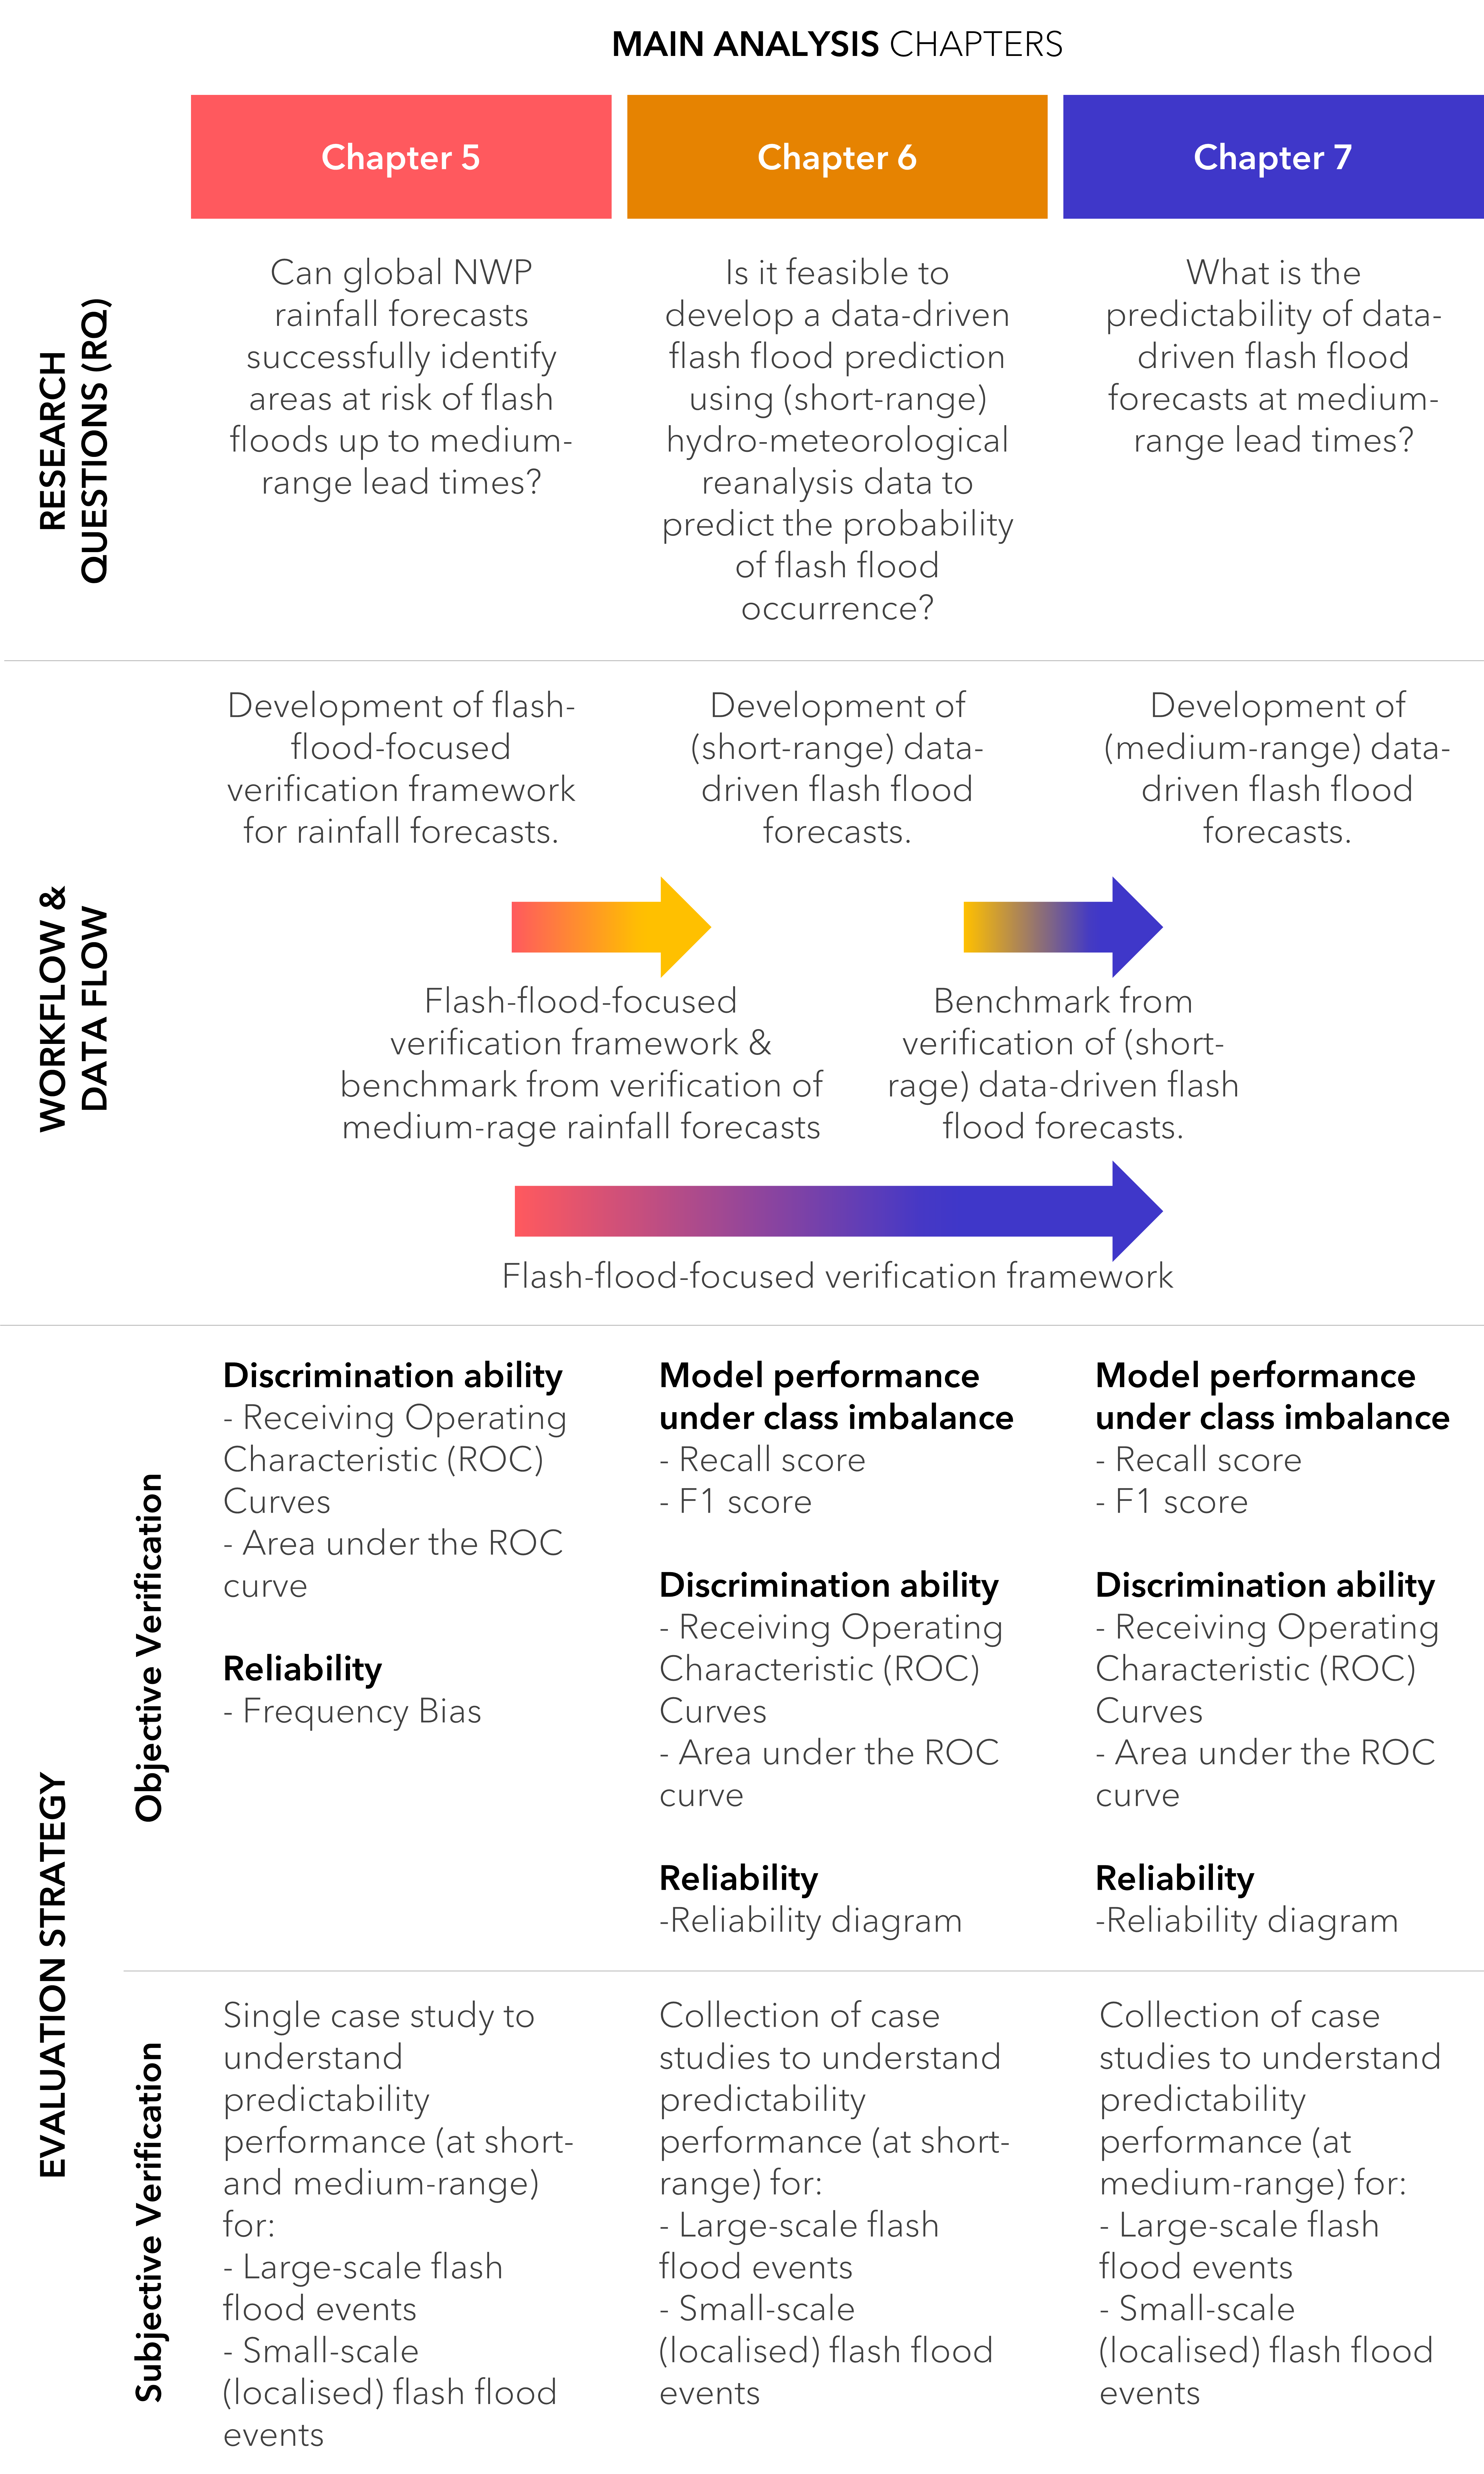
\includegraphics[width=\textwidth]{workflow_dataflow.png}
\caption{\textbf{Overview of the experimental design across the "Main Analysis" chapters (5 to 7).} The infographic delineates the research questions addressed in each chapter, the workflow of data flow across the chapters, and the adopted evaluation strategies to assess the performance of global NWP rainfall forecasts and data-driven flash flood predictions in identifying areas at risk of flash floods.}
\label{fig:workflow_dataflow}
\end{figure}

The \marginpara{Third methodological component (addressing RQ3): development of medium-range data-driven hydro-meteorological predictions of areas at risk of flash floods - Regional and global prototype} third methodological component extends the application of the data-driven model to medium-range forecasts, enabling the assessment of flash flood predictability beyond typical short-range (day 0) predictions. This component synthesises the findings from the previous two methods, applying the data-driven framework developed in the second stage to longer-range forecast data and the verification framework developed in the first stage of the analysis to evaluate how predictive skill for flash flooding decays with increasing lead times. This evaluation is crucial for understanding the temporal limitations of actionable flash flood predictions.



The following sections will detail each methodological component, including data sources, processing techniques, model development procedures, and verification frameworks adopted in this study. 

data sources (which component relates to), make it look like I thought it all together.

ADD THE CROSS REFERENCING ALL OVER THE THESIS TO AVOID REPETITIONS OR TOO MUCH DETAIL.


%%%%%%%%%%%%%%%%%%%%%%%%%%%%%%%%%%%%%%%%%%%%%%%%%%%%%%%%%%%%%%%%%%%%%%%%%%%%
\section{Flash-flood-focused verification framework}

\begin{figure}[htbp]
\centering
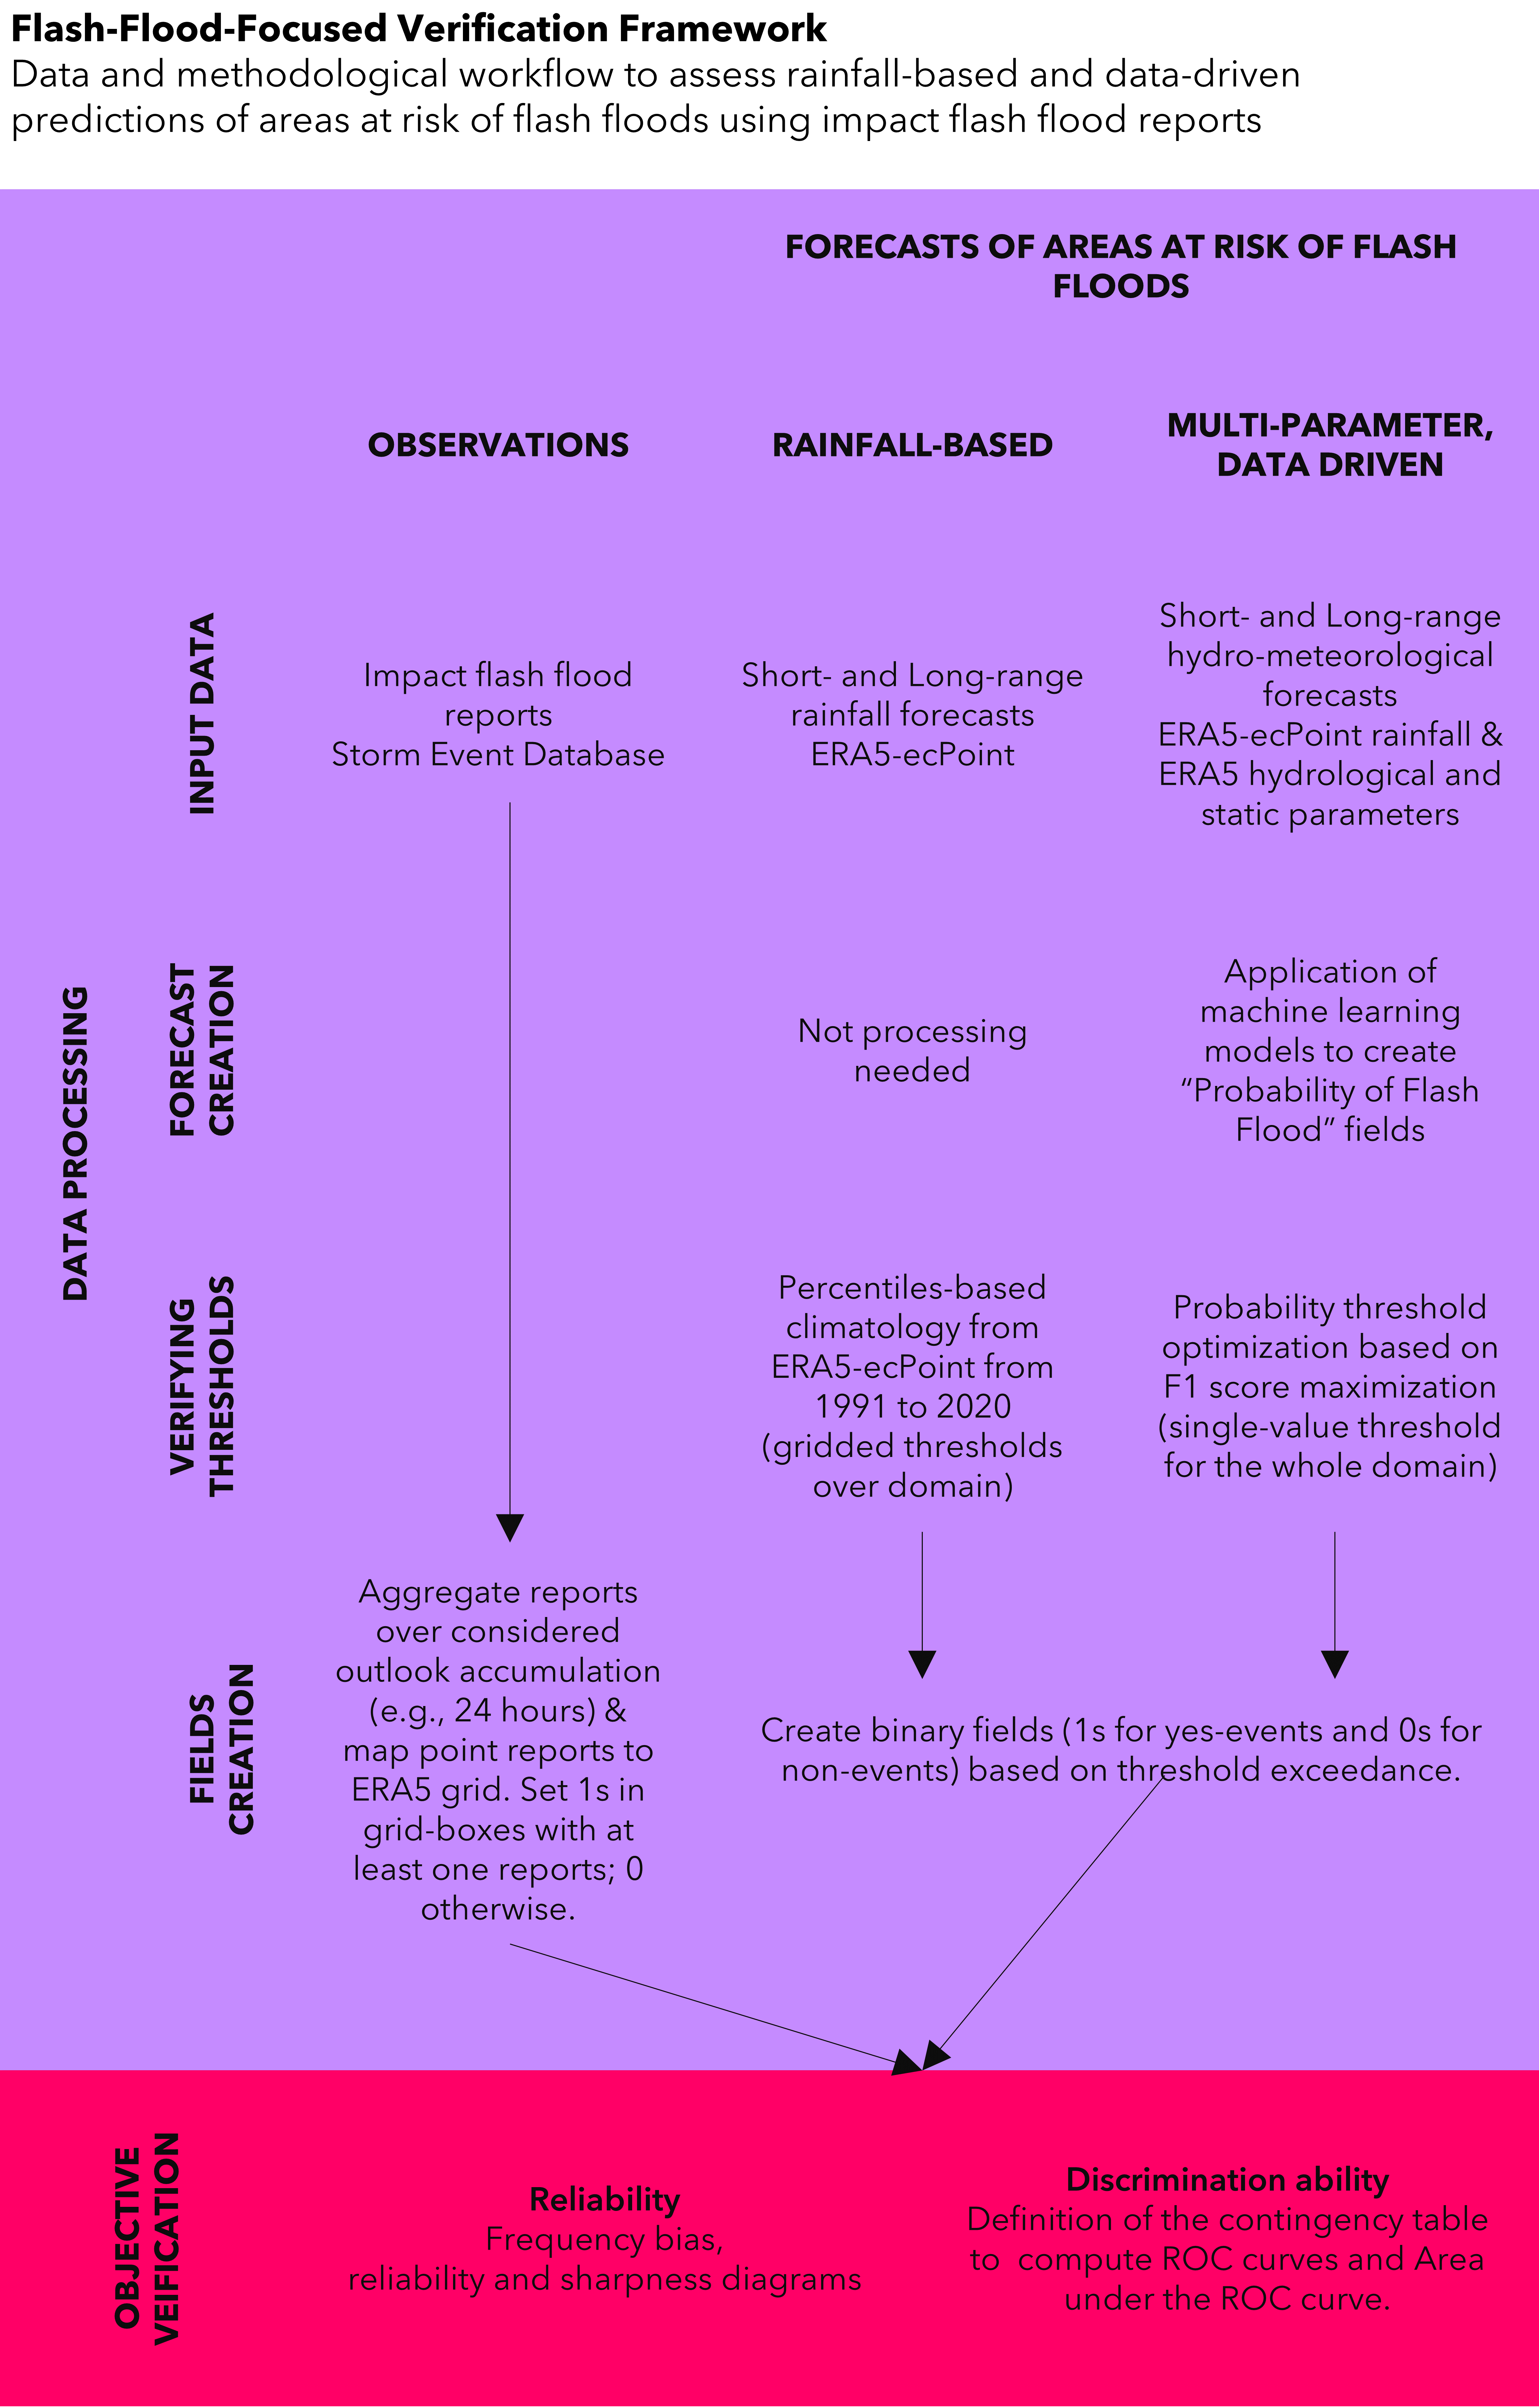
\includegraphics[width=\textwidth]{workflow_verif_framework.png}
\caption{\textbf{Workflow for flash-flood-focused verification framework.} Data and methodological framework to assess predictions of areas at risk of flash floods using impact flash flood reports.}
\label{fig:workflow_verif_framework}
\end{figure}

\subsection{What observational data are required for flash flood verification?}

The selection of appropriate observational data constitutes a critical foundation for any verification framework. This study utilises the Storm Events Database, maintained by the National Oceanic and Atmospheric Administration (NOAA), as the primary source of flash flood observations across the Continental United States (CONUS). This database represents the most comprehensive and systematically maintained record of flash flood impacts available at continental scale, containing detailed spatio-temporal information for events from 1950 to the present (purple area in Figure \ref{fig:workflow_verif_framework}).

The choice of an impact-based database rather than hydrological measurements reflects the fundamental nature of flash floods as localised phenomena occurring predominantly in ungauged catchments. Traditional gauge-based observations fail to capture the majority of flash flood events due to their sparse spatial distribution and the rapid onset characteristics of these events. Impact databases, whilst subject to reporting biases, provide a more feasible approach for continental-scale verification where the installation and maintenance of dense observational networks remains economically and logistically prohibitive.

The Storm Events Database offers several advantages that justify its selection. First, it provides consistent reporting standards across all US states, enabling uniform analysis across diverse hydro-climatic regions. Second, each report includes precise geolocation data, essential for grid-based verification approaches. Third, the database undergoes quality control procedures by NOAA, reducing, though not eliminating, reporting inconsistencies that might be present in other databases such as ESWD (with clear reporting biases over Germany). These characteristics make it the most suitable dataset for establishing a robust verification framework, acknowledging that similar approaches could be applied to other regional databases such as the European Severe Weather Database or global repositories like EM-DAT and Desinventar, each with their specific limitations and biases.


\subsection{Why using ERA5 and ERA5-ecPoint data in the development of predictions of areas at risk of flash floods?}

The ERA5 dataset was selected in this thesis as it provides a long-term (from the 1950s to the present), high-quality reconstruction of hydro-meteorological fields over a continuous global domain \citep{Hersbach_2020}. Thus, the short-range forecasts (up to day 0, and also known as \textit{reanalysis}) provide a good dataset for the training of the data-driven predictions. While ERA5 provides a consistent dataset for training over space and time, its coarse resolution makes raw ERA5's rainfall estimates not appropriate for flash flood applications as localised rainfall peaks tend to be underestimated, and severely underestimated in the case of isolated convection. For this reason, the rainfall estimates used for training and verification come from the post-processed ERA5 rainfall estimates with the ecPoint methodology, which provides a probabilistic distribution of how the localised extreme rainfall estimates might be. A more detailed description of the post-processing methodology and the quality of the ecPoint rainfall forecasts can be found in section \ref{ecpoint_rainfall}.

Regarding the longer-range forecasts used to create the medium-range predictions of areas at risk of flash floods, it is common practice to fine-tune the training done with lower-resolution datasets (such as ERA5, at 31 km) to the higher resolution of typically used forecasting systems (such as ECMWF's IFS, at 9 km). In the field of data-driven weather forecasts, this is done in the AIFS, which is trained over ERA5 and fine-tuned over the operational analysis at 9 km to obtain forecasts with a spatial resolution of \sim25 km  \citep{Lang_2024}. This approach was not adopted in this thesis as it would introduce uncertainties in the forecasting chain related to such fine-tuning that would be difficult to dissociate from uncertainties due to the prediction of the hazard itself. Hence, the long-range forecasts from ERA5 and corresponding ecPoint post-processed rainfall estimates were used in this thesis. Even though this approach means creating a low-resolution prototype for flash flood prediction (as the medium-range forecasts remain provided at 31 km resolution), the forecast uncertainties presented in this thesis remain detached from fine-tuning processes and can be related primarily to the physical processes that generate flash floods and the data used to create the short- and medium-range forecats.

\subsection{How should flash flood observations be processed for grid-based verification?}

The transformation of point-based impact reports into gridded observational fields requires careful consideration of spatial and temporal aggregation methods. This study implements a systematic approach aligned with established severe weather verification methodologies \citep{Tsonevsky_2018, Pillosu_2024}.

Each flash flood report undergoes temporal aggregation to match the 24-hour accumulation periods of the forecast products, beginning at 00 UTC. This alignment ensures consistent comparison between observations and predictions whilst acknowledging that flash floods may occur at any time within the accumulation window. The choice of 24-hour periods balances the need for sufficient temporal resolution with the practical constraints of forecast product availability and the typical duration of flash flood events.

Spatial assignment of reports to the ERA5 grid (approximately 31 km resolution) employs a nearest-neighbour approach for point reports and polygon inclusion for events with spatial extent. Given the relatively coarse resolution of ERA5 grid boxes compared to typical flash flood scales, additional spatial expansion techniques commonly used in convective-scale verification prove unnecessary. The resulting gridded fields preserve information about event frequency within each grid box, enabling more nuanced verification than binary occurrence fields.
This processing approach addresses the fundamental challenge of scale mismatch between localised flash flood events and gridded forecast products. The methodology provides a reproducible framework applicable to other grid resolutions and accumulation periods, with detailed implementation provided in chapter \ref{flash_flood_focused_verification_framework}.


\subsection{What verification thresholds enable meaningful assessment of flash flood predictions?}

The establishment of appropriate verification thresholds represents a critical methodological decision that directly influences all subsequent analyses. 

For rainfall-based predictions, thresholds must reflect the precipitation amounts capable of generating flash floods across diverse hydro-climatic conditions. In the absence of comprehensive observational networks capturing extreme precipitation at flash flood scales, this study develops a novel approach using ERA5-ecPoint rainfall estimates. ERA5-ecPoint provides bias-corrected, post-processed rainfall estimates that better represent point-scale extremes compared to raw ERA5 data \citep{Pillosu_2025a}. A 30-year climatology (1991-2020) following WMO standards enables the derivation of location-specific rainfall thresholds corresponding to various return periods. This approach captures the spatial heterogeneity of flash flood susceptibility, recognising that identical rainfall amounts may produce vastly different impacts depending on local conditions. The selection of multiple threshold percentiles allows examination of forecast performance across the full spectrum of flash flood severity. Lower percentiles capture more frequent, lower-impact events, whilst higher percentiles focus on rare, catastrophic floods. This multi-threshold approach provides insights into how forecast skill varies with event rarity and severity, essential information for operational implementation where different stakeholders may have varying risk tolerances.

For hydro-meteorological, data-driven predictions, the verifying thresholds emerge directly from the machine learning algorithms that generated the predictions themselves, applying an optimisation that establishes the probability values that maximise the F1-score when converting a probabilistic prediction into a yes- or non-event. This data-driven threshold selection represents a departure from traditional approaches based, for example, on assumptions about the severity of the triggering events (as done for the rainfall-based forecasts). It instead allows the data-driven models itself to identify optimal decision boundaries to convert the probabilistic forecasts into a yes- or a non-event. As such, the thresholds will be defined based on the frequency of the yes-events in the observational datasets, delivering smaller verifying thresholds for rarer events. 


\subsection{Which verification metrics provide a comprehensive assessment of forecast quality?}

The verification framework employs a suite of metrics designed to evaluate different aspects of forecast performance, recognising that no single metric can fully characterise prediction quality for rare events like flash floods (pink area in Figure \ref{fig:workflow_verif_framework}). The selection of metrics addresses two primary forecast attributes: reliability and discrimination ability.

Reliability assessment examines whether predicted probabilities accurately reflect observed frequencies. The frequency bias provides an aggregate measure of systematic over- or under-prediction, whilst reliability diagrams offer detailed insights into calibration across the full probability spectrum. These metrics prove particularly valuable for understanding how well forecast systems capture the climatological frequency of flash floods, a fundamental requirement for risk-based decision making.

Discrimination ability quantifies the forecast system's capacity to distinguish between flood and non-flood situations. The Area Under the Receiver Operating Characteristic curve (AROC) provides a threshold-independent summary measure, whilst the full ROC curve reveals performance trade-offs at different probability thresholds. For rare event prediction, discrimination ability often represents the primary challenge, as models must identify subtle signals preceding infrequent occurrences.

The choice of probabilistic metrics reflects the inherent uncertainty in flash flood prediction and the need for risk-based decision frameworks in operational contexts. Deterministic metrics prove less suitable given the rarity of events and the importance of capturing forecast uncertainty. Detailed mathematical formulations and computational procedures are provided in the relevant analysis chapters.

%%%%%%%%%%%%%%%%%%%%%%%%%%%%%%%%%%%%%%%%%%%%%%%%%%%%%%%%%%%%%%%%%%%%%%%%%%%%%%%%%
\section{Development of data-driven predictions of areas at risk of flash floods}


\subsection{How can data-driven models address the extreme class imbalance in flash flood data?}

The development of data-driven flash flood prediction models must confront the fundamental challenge of extreme class imbalance, with flash flood events representing approximately 0.2\% of the observational dataset. This imbalance poses significant challenges for machine learning algorithms, which may converge to trivial solutions that never predict positive events.

This study adopts ensemble learning techniques as the primary strategy for addressing class imbalance. Unlike data-level approaches that modify the training dataset through over- or under-sampling, ensemble methods preserve the original data distribution whilst improving minority class detection through algorithmic diversity. This choice reflects a deliberate decision to maintain the integrity of the observational dataset, avoiding the introduction of synthetic samples or the loss of potentially informative negative examples.

The experimental design incorporates multiple ensemble algorithms, including Random Forest, Gradient Boosting variants (XGBoost, LightGBM, CatBoost), neural networks, and ensemble stacking. Each algorithm offers different mechanisms for handling imbalanced datasets, from the inherent bootstrap sampling in Random Forest to the sequential error correction in boosting methods. This diversity enables a comprehensive assessment of which algorithmic approaches best suit the flash flood prediction challenge.


\subsection{What training strategy ensures robust assessment of model performance when working with an extremely imbalanced dataset?}

The validation framework employs nested cross-validation with hyperparameter optimisation to provide unbiased performance estimates whilst maximising model performance. This approach addresses the risk of overfitting inherent in machine learning applications to imbalanced datasets.

The outer cross-validation loop uses stratified k-fold splitting to ensure representative class distributions in all data partitions. Within each outer fold, an inner optimisation loop identifies optimal hyperparameters using Bayesian optimisation via the Optuna framework. This nested structure prevents information leakage between hyperparameter selection and performance evaluation, providing realistic estimates of operational performance.
The choice of AROC as the optimisation metric during hyperparameter tuning reflects its suitability for imbalanced classification and alignment with the verification framework. Alternative metrics such as F1-score prove less suitable due to their dependence on classification thresholds and potential instability with extreme class imbalance.

Repeated evaluation across multiple cross-validation folds quantifies performance variability and identifies potential instabilities in model training. This comprehensive validation approach ensures that reported performance metrics reflect genuine predictive capability rather than fortunate data splits or overfitting to specific training samples. Implementation details and computational considerations are discussed in Chapter \ref{feasibility_PoFF}.
       % Chapter 3
% %%%%%%%%%%%%%%%%%%%%%%%%%%%%%%%%%%%%%%%%%%%%%%%%%%%%%%
\chapter{Experimental design}
\label{experimental_design}
\graphicspath{{chapter_04/figures}{chapter_04/tables}}
%%%%%%%%%%%%%%%%%%%%%%%%%%%%%%%%%%%%%%%%%%%%%%%%%%%%%%


\section{Development of a flash-flood-focused verification framework}

This study faces two main challenges. The first challenge consists in the definition of the verifying thresholds that will be used to assess the performance of the rainfall-based and multi-parameter-based, data-driven predictions of areas at risk of flash floods. The second challenge consists of the use of appropriate verification scores due to the intrinsic characteristic of the observational datasets as it is not possible to define univocally observational yes- and non-events. 

In this section, we define a \textit{flash-flood-focused verification framework to assess (short- and medium-range) predictions of areas at risk of flash floods}. This framework will be used throughout the thesis to assess the performance of the rainfall-based flash flood forecasting system and its multi-parameter counterpart provided here by both data-driven models, the short-range (computed with the short-range ERA5 and ERA5-ecPoint forecasts) and the medium-range (computed with the equivalent long-range forecasts up to day 5). The application of the flash-flood-focused verification framework to the identification of areas at risk of flash floods involving solely rainfall predictions is done in the recognition that a robust understanding of rainfall forecast performance in identifying areas at risk of flash floods is essential to benchmark the performance of more advanced prediction methods, e.g. data-driven approaches involving more parameters.

The objective verification framework uses flash flood impact observations as ground truth. As indicated in section \ref{storm_event_database}, this thesis will consider only the Storm Event Database over the CONUS. However, this method can be applied in other geographical regions where regional databases are available, such as over Europe (using the ESWD dataset) or a global domain (considering global datasets such as EM-DAT), while always acknowledging the biases that such impact databases might possess. 


\subsection{Observational fields}
The definition of the observational dataset follows the methodology proposed by \citep{Tsonevsky_2018} for severe weather, and \citep{Pillosu_2024} for flash floods in Ecuador. Each flash flood report must first be grouped with all the reports belonging to the accumulation period for which the flash flood outlooks are provided. This thesis provides predictions of areas at risk of flash floods over 24-hourly accumulation periods starting at 00 UTC. Hence, this step's outcome consists of the list of \textit{point} flash flood reports happening between the 1st of January at 00 UTC and the 2nd of January at 00 UTC, between the 2nd of January at 00 UTC and the 3rd of January at 00 UTC, etc. 

Each point report in a specific accumulation period must then be located on the ERA5 grid-box where the event happened. In the Storm Event Database, the location of each flash flood event is provided by two latitude coordinates ("BEGIN\_LAT" and "END\_LAT") and two longitude coordinates ("BEGIN\_LON" and "END\_LON"). If BEGIN\_LAT = END\_LAT and BEGIN\_LON = END\_LON, the flash flood event is identified by a single point, and only the closest grid-box to that point is assigned the flash flood event using the "nearest grid-box" method. If BEGIN\_LAT \ne END\_LAT and BEGIN\_LON \ne END\_LON, a polygon is provided in all grid-boxes within that polygon get assigned the flash flood event. It is worth noting, that even when a polygon is provided, only one grid-box might contain the flash flood event is the radius of the event was not bigger than the ERA5's grid-boxes resolution, i.e., 31 km. This procedure creates \textit{gridded} fields of flash flood reports, where the values assigned to the grid-boxes indicate the number of flash flood reports occurred within the grid-boxes, e.g. a grid-box with 0 does not contain any flash flood reports for the considered accumulation period, while a grid-box with a value of 5 indicates that there are 5 flash flood reports within that grid-box, for the considered accumulation period.

Because of the large size of the ERA5 grid-boxes (i.e., 31 km) and the large accumulation periods for the flash flood outlooks (i.e. 24 hours), any additional expansion in the area or reporting times of individual reports is probably unnecessary to account for uncertainties in the location and reporting times. It is possible to envision remote scenarios in which a report is close enough to the edge of the ERA5 grid-box or the outlook accumulation period that a location or reporting time error in the database could cause the mislocation of such flash flood event, but this scenario has been established to be for ~0.1\% of the total number of the reports considered in this thesis, so no further methodologies will be considered here to account for uncertainties in the location or reporting time in the Storm Event Database. 

Figure \ref{fig:sed_reports} shows an example of the post-processed flash flood reports from the Storm Event Database.

\begin{figure}[htbp]
\centering
\includegraphics[scale=0.65]{sed_reports.png}
\caption{\textbf{Example of post-processed reports from the Storm Event Database.} Panel (a) shows the timeseries of the counts of all flood types recorded in the database from January 1950 to December 2023 (in grey), the counts of all flash floods recorded (in dark red), and the counts of all flash floods records including lat/lon coordinates (in red). Panel (b) shows the timeseries of point (in red) and gridded (in black) flash flood reports in 2021, accumulated over 12-hourly accumulation periods ending at 00 and 12 UTC. Panel (c) shows the spatial distribution of point flash flood reports (in red) during the 12-hourly accumulation period ending on 2021-09-02 at 00 UTC (i.e. for storm Ida). The zoomed in area shows an example of the number of point flash flood reports (in red) assigned to the nearest grid-box. Those grid-boxes containing at least one point flash flood reports is coloured in black. Panel (d) shows the spatial distribution of the observed frequency of flash flood events in each grid-box between 2005 and 2023. A distinction between four main areas is applied: the probabilities in the north-west, north-east, south-east and south-west are indicated, respectively, in orange, turquoise, cyan, and green. The probabilities are discretised in equal to 0\% (in white for all the regions), between 0-0.1\%, 0.1-1\%, and 1-10\% (in different tones of the colour for the corresponding region). Panel’s (d) insert shows a piechart representing the proportion of gridded flash flood reports in each considered region.}
\label{fig:sed_reports}
\end{figure}


\subsection{Forecast fields}

Given a forecast value at a grid-box, a flash flood event is considered as a yes-event if the forecast exceeds a specific event threshold (whose definition is explained in section \ref{verifying_rainfall_threshold}). The forecast fields are then created by assigning the value 1 to all those grid-boxes where the forecasts exceed the considered threshold; otherwise, the value 0 is assigned. 

\subsection{Definition of the verifying thresholds}
\label{verifying_rainfall_threshold}
For the rainfall-based predictions of areas at risk of flash flood, a rainfall-based threshold must be used. For the verification of rainfall-based predictions of areas at risk of flash floods, flash-flood-triggering rainfall totals might be known for the region of interest, so that they can be used as thresholds to define the flash flood events to verify. In this thesis, such rainfall thresholds are not know for the CONUS, and therefore, must be computed from data. If point rainfall observations are available (e.g., rain gauges or radars), one can create the distribution of the observed flash-flood-triggering rainfall totals, and the verifying rainfall thresholds (VRT) values would then correspond to the specific percentiles of the distribution. The higher the percentile, the higher the magnitude of the VRT, and the higher the severity level of flash flood events considered in the objective verification analysis. This approach requires high-density rainfall observations, in both space and time, to capture the localised extreme rainfall totals that trigger flash floods \citep{Haiden_2016, RamosFilho_2021}. In the absence of a suitable observational network, the VRT values can be defined only from gridded rainfall products such as reanalysis e.g., ERA5 \citep{Hersbach_2020}, reforecasts \citep{Hamill_2006b}, or blended rainfall observations provided on a grid such as MSWEP \citep{Beck_2019} or GPCP \citep{Adler_2018}. These datasets, however, tend to underestimate rainfall extremes because of their coarse spatial resolution \citep{Tapiador_2019}. In the absence of more suitable gridded datasets, \citet{Pillosu_2024} proposed a methodology to compute regional point rainfall climatologies using 1 year of short-range (day 1) ecPoint rainfall forecasts. This approach, however, has the disadvantage to use only 1 year of forecasts, which means that the resulting climatologies will inevitably be affected by the climatology of that specific year instead of the general climatology of the region that they are supposed to represent. Moreover, as this climatology requires flash flood observations to be defined, and such observations tend to have an even lower resolution than rainfall forecasts, there is the need to create climatologies for large domains, rather than on a grid-box scale. For example, \citet{Pillosu_2024} created only two verifying rainfall thresholds for Ecuador, one for the coastal and one for the Andean region. While this disaggregation is better than having one single value for an entire country, regional thresholds might not be able to capture flash-flood-triggering rainfall thresholds over different micro-climates. This would not allow an appropriate disaggregation of the performance of the flash flood forecasts in different regions, under different (hydro-meteorological) conditions. Hence, in this thesis, we propose the definition of the rainfall VRTS from a climatology built with ERA5-ecPoint rainfall estimates, as they have been shown to represent point-rainfall climatologies around the world reliably \citep{Pillosu_2025a} and they would allow us to develop a grid-box scale rainfall climatology to be used as thresholds for the rainfall-based predictions of areas at risk of flash floods. Hence, an ERA5-ecPoint rainfall climatology has been computed over the WMO recommended 30-year period 1991-2020 \citep{WMO_2017}. Table \ref{} shows the percentiles and corresponding values as x-year return periods that have been considered as flash-flood-triggering rainfall events during the verification.


\subsection{Objective verification}

The objective verification carried out in this thesis is based of verification scores computed through a probabilistic contingency table. We follow \citet{Pillosu_2024} methodology for the population of the contingency tables. Stationary observations (i.e. provided by instruments installed at a specific location, such as rain gauges, provide timeseries of yes- and non-events recorded at the location where the instrument was installed. THus, all four elements in the contingency table can be quantified. Non-stationary observations record only yes-events at the location where the event occurred. As a result, it is impossible to answer the question "if there are no reports in an area, is it because an event happened but nobody reported it, or because there was no event to report?". Some studies facing the same problem because they use non-stationary observations such as impact reports, verify only yes-events with the caveat that only quadrant I (i.e. hits) and III (i.e. misses) of the contingency table can be populated \citep{Robbins_2018}. Instead, this study followed the method proposed by \citet{Tsonevsky_2018}, which allows to populate all quadrants of the contingency table. This method assumes that a non-reports corresponds to a non-event. 

Hence, the contingency tables are built by examining overlapping grid boxes in correspondent observational and forecast fields. When both grid-boxes are assigned a value of 1 or 0, they count as a hit or a correct negative, respectively. When a grid-box in the observational field is assigned a value of 1, and the corresponding grid-box in the forecast field is assigned a value of 0, it counts as a miss. It counts as a false alarm if the opposite occurs. 


\subsection{Properties of probabilistic forecasts}

Reliability and discrimination ability are desirable properties of ensemble forecasts, and both are defined against a verifying threshold \citep{Jolliffe_2012, Wilks_2020}. Reliability measures whether the chosen verifying threshold is predicted with probabilities that mirror the frequency with which the considered event is observed. Discrimination measures the forecasts' ability to distinguish situations that lead to events exceeding the verifying threshold from those that do not, appraising the existence of a signal in forecasts when an event materialises. In this thesis, we consider two types of scores to analyse reliability and discrimination ability: summary and breakdown scores. Summary scores show the overall reliability and discrimination ability of the forecasts, while the breakdown scores provide detailed insights into how reliability and discrimination ability relate to the full distribution of probabilities. 


\subsubsection{Reliability}

To assess the overall reliability of the forecasts, we will consider the frequency bias (FB) to evaluate the overall reliability of the predictions of areas at risk of flash floods. The frequency bias was determined by dividing the total number of yes-events in the forecasts by the total number of yes-events in the observations. FB values range from 0 to $+\infty$. FB = 1 indicates perfect calibration, while scores greater or smaller than 1 indicate, respectively, over- and under-prediction of the observed yes-events. It is worth noting that FB measure the overall ratio of forecasts events to observed events and is not a measure of forecast sill. As such, it can provide a score of 1 when there are compensating error. Moreover, FB might show large overestimations if the observed event is heavily underreported. This is our case as explained in section \ref{fig:sed_reports}.

To break down the reliability of the forecasts over the full distribution of probabilities, reliability diagrams are used. They plot the relative forecasts probability of an event against its corresponding relative observational frequency, indicating how reliable the forecast probabilities are at different classes. For perfect forecasts, when the forecasts show x\% probability of occurrence, observations should meet the criteria x\% of the time, so that the reliability curve lies on the diagonal. If the reliability diagram is above the diagonal for a specific forecast probability, those forecasts are under-predicting the likelihood of observing a yes-event. If it lies below the diagonal, the is over-prediction. When analysing reliability diagrams, it is also important to know the frequency distribution of forecasts issued with specific probabilities. For example, the small probability thresholds (within the red box in the figure example) are the most important when considering high verifying thresholds because the sample of forecasts exceeding the verifying threshold with high probabilities is rather small. For this reason, reliability diagrams should be accompanied by sharpness diagrams, which plot the absolute frequency of forecasts of different probabilities. 


\subsubsection{Discrimination ability}

Relative Operating Characteristic (ROC) curves are built from 2x2 contingency tables (Table \ref{}), quantifying hits (H) misses (M) false alarms (FA), and correct negatives (CN). Hit rates (HR) and false alarm rates (FAR) are computed, respectively from equations:




HRs are mapped (Y-axis) against FARs (X-axis) in a unit square. The form of the ROC curve shows how HRs vary with FARs as one systematically lowers the thresholds probability at which it is assumed that an event has technically been forecast to happen (i.e. 100\% of probability the bottom left corner to 0\% probability at the top right corner). The values of the geometrical area under the ROC curve (AROC) provide a summary measure of the discrimination ability across all probability thresholds. The plot of AROC values for different lead times allows us to compare the discrimination ability between the rainfall-based predictions of areas at risk of flash floods, and the multi-parameter-based, data-driven predictions, (both at short- and medium-range lead times). Perfect discrimination is obtained when only HRs grow and FARs remain zero. It is represented by a ROC curve that rises along the Y-axis from the bottom left corner of the unit square to the top-left corner and moves straight to the top-right corner. In this case, the AROC is equal to 1. If HRs and FARs grow at the same rate, the forecasts have no discrimination ability (as a climatological forecast). In this case, the ROC curve lies along the diagonal and AROC equals 0.5. 

How ROC curves and AROCs are computed can impact the interpretation of forecasts discrimination ability. For rainfall-based predictions, the ROC curves will be built for incremental decision thresholds that are materially assessable from the real ensemble configuration. In this way, we can estimate the "real" forecast discrimination ability \citep{wilks_statistical_2020}. Probability thresholds are determined by considering the full discretisation ability in the ensemble (e.g., 99 members in the case of ERA5-ecPoint). This ensures that the ROC curves are as complete as possible \citep{Bouallegue_2022}. The number of thresholds corresponds, therefore, to the number of members exceeding the verifying rainfall threshold so that for an enmble of size M, maximum discretisation is achieved by M+1 probability thresholds (i.e., 0, 1/M, 2/M, ...., M/M=1). For the data-driven forecasts, where the forecast probability is provided by the model with continuous numbers between 0 and 1, the decision (probability) thresholds are defined by the user. In this thesis, a discretisation of 0.01 (equivalent to 1\%) and 0.001 (equivalent to 0.1\%) will be considered given the low frequency observed of flash flood events in the observational database. The ROC curve is then built by straight segments joining successive points. It is then completed by joining that last meaningful point with a straight line in the top-rigth corner of the unit square. FOr rare events, the points of a ROC curve cluster in the graph's bottom left corner and completing the ROC with a straight line might give the impression that part of the curve is missing \citep{Casati_2008}. How much the curve appears incomplete depends on the ensemble size and the base rate of the event. The area under the ROC curve (AROC) will be computed using a trapezoidal approximation by adding the areas of single trapeziums formed by the straight lines between consecutive points in the ROC curve \citep{Bouallegue_2022}. 

From what written before, the ROC curves represent the breakdown measure of discrimination ability as it will be possible to examine the values of HRs and FARs at different decision (probability) thresholds. AROC will represent instead the overall measure of discrimination ability.

       % Chapter 4
% %%%%%%%%%%%%%%%%%%%%%%%%%%%%%%%%%%%%%%%%%%%%%%%%%%%%%%%%%%%%%%%%%%%%
\chapter{Results}
\label{results}
\graphicspath{{chapter_05/figures}{chapter_05/tables}}
%%%%%%%%%%%%%%%%%%%%%%%%%%%%%%%%%%%%%%%%%%%%%%%%%%%%%%%%%%%%%%%%%%%%

This chapter presents the findings of the research carried out in this thesis to assess how effectively different forecasting methodologies (i.e., rainfall-based forecasts or data-driven approaches combining hydro-meteorological data) identify areas at risk of flash floods, and what predictability we should expect from both systems.

The analysis progresses through three interconnected components that collectively establish the current capabilities and future potential of the above-described flash flood prediction systems. 

Our research starts with the flash-flood-focused evaluation of short- and long-range rainfall estimates from ERA5-ecPoint. These post-processed estimates have been shown to represent better than ERA5 extreme rainfall estimates at point-scale, making it an ideal candidate for establishing baseline predictive capabilities across diverse geographical and climatological contexts \citep{Pillosu_2025a}. While such improvement in the prediction of localised extreme rainfall should enable improved detection of areas at risk of flash floods, the flash-flood-focused assessment is fundamental to determine a baseline to compare more sophisticated prediction systems, such as the data-driven approach that combines hydro-meteorological parameters.

Building upon this foundation, the second analytical component introduces a data-driven approach integrating hydro-meteorological parameters to enhance flash flood prediction. Whilst rainfall's magnitude, duration, and location are critical factors, flash flood occurrence depends upon complex interactions between meteorological forcing and catchment characteristics, including antecedent soil moisture conditions, topographical features, and land cover. The data-driven model developed herein incorporates these factors to capture the nonlinear relationships that govern flash flood generation, moving beyond purely meteorological prediction towards a more holistic hydro-meteorological framework.

The temporal dimension of forecast skill forms the third pillar of this analysis. Understanding how predictive capability degrades with increasing lead time is paramount for operational implementation, as it determines the practical warning times available to emergency managers and at-risk communities. This temporal analysis extends up to 5 days ahead, encompassing the full range of lead times relevant to flash flood preparedness and response activities. Day 1 forecasts would be used to activate emergency operation centres, pre-position resources in high-risk areas, and issue public warnings through media channels. Day 2-3 forecasts would be used to support broader preparedness activities, including mobilising regional resources, implementing precautionary evacuations in highly vulnerable areas, and allowing businesses and schools to adjust operations. Day 4-5 forecasts, whilst containing greater uncertainty, permit strategic planning such as adjusting reservoir operations, preparing emergency shelters, and enabling voluntary protective actions by residents, and although forecast skill diminishes at these lead times, the information remains valuable for initial situational awareness. By quantifying skill degradation across different forecast horizons, this analysis establishes realistic expectations for early warning systems and identifies the temporal windows within which different decision-making processes can be reliably supported.

Throughout this thesis, the flash-flood-focused verification framework described in section \ref{flash_flood_focused_verification_framework} has been applied to both rainfall-based and data-driven forecasts of areas at risk of flash floods to ensure comparability across approaches and lead times. The study utilises observational flash flood records from NOAA's Storm  Event Database across the contiguous US (CONUS), validated against ERA5-ecPoint rainfall forecasts and the data-driven hydro-meteorological predictions. Performance metrics include frequency bias and reliability diagrams to assess forecasts' reliability, and ROC curves and the estimation of the areas under the ROC curves to assess the predictions' discrimination ability. 

The results presented in the subsequent sections document the performance of both rainfall-based and data-driven hydro-meteorological forecasts. Section \ref{verif_rainfall_based_fc} shows the baseline verification results for the prediction of areas at risk of flash floods based using only ERA5-ecPoint short- and long-range rainfall predictions. Section \ref{verif_data_driven_short_fc} shows that the data-driven approach combining hydro-meteorological parameters yields statistically significant improvements in prediction skill, with particularly notable gains in discrimination ability as seen in the provided ROC curves. Section \ref{verif_data_driven_long_fc} shows that the predictive skill of the data-driven forecasts extends to day 5 with my better discrimination ability than its only rainfall-based counterpart. Section \ref{verif_case_study} shows a selection of flash flood events to illustrate the approaches' capacity to identify areas at risk of flash floods (in the US and around the world). Hence, the findings detailed in this chapter contribute to understanding how effectively current technologies can support flash flood warning systems.



%%%%%%%%%
\section{Assessment of rainfall-based predictions of areas at risk of flash floods}
\label{verif_rainfall_based_fc}

\subsection{Overall verification scores: frequency bias and area under the ROC curve}

\begin{figure}[htbp]
\centering
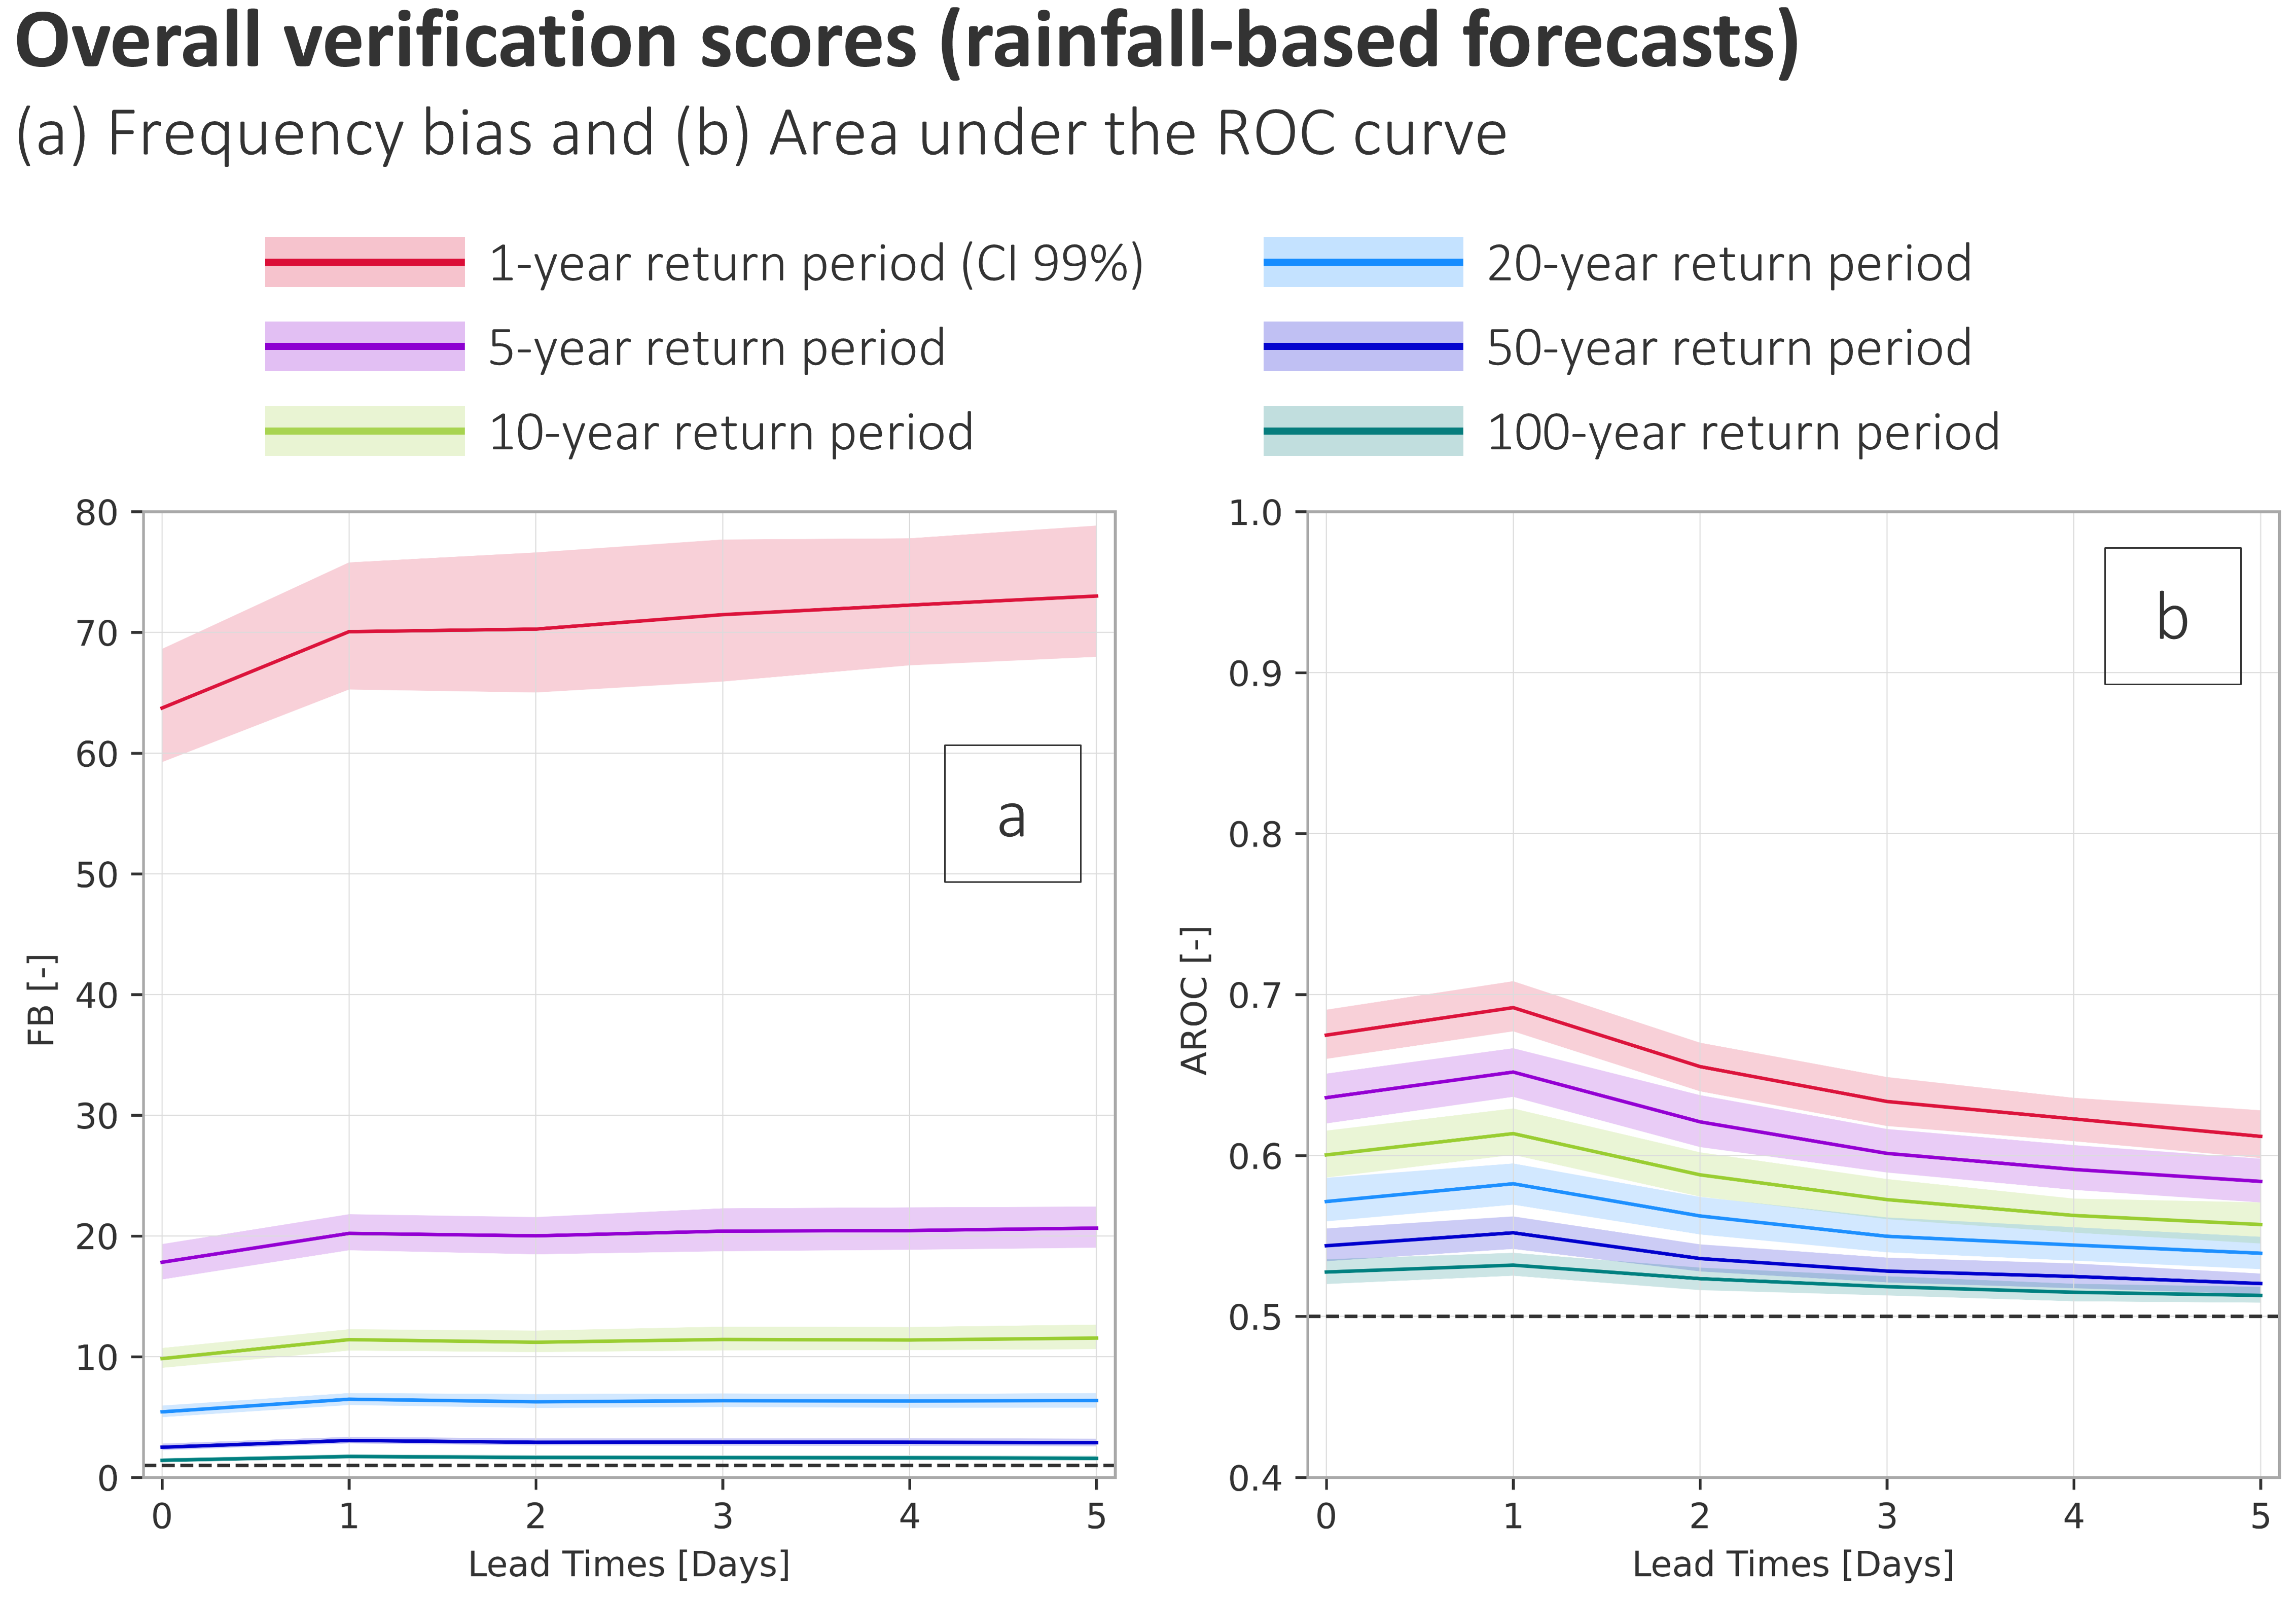
\includegraphics[width=\textwidth]{chapter_05/figures/rainfall_based_ff_verif_overall_scores.png}
\caption{\textbf{Overall verification scores for the rainfall-based forecasts of areas at risk of flash flood.} Panel (a) shows the frequency bias (solid lines) for 1-year (in red), 5-year (in purple), 10-year (in light green), 20-year (in cyan), 50-year (in blue), and 100-year return period (in green). The corresponding shaded areas represent the confidence intervals at 99\% confidence level. The inset box contains a zoomed-in version of the panel to show better the frequency bias values close to 1 (representing perfect bias). Panel (b) shows the area under the ROC curve.}
\label{fig:rainfall_based_ff_verif_overall_scores}
\end{figure}


\subsection{Discrimination ability}

All forecasts for rainfall events exceeding the 1-year return period threshold (Figure \ref{fig:rainfall_based_ff_verif_breakdown_scores_roc_1rp}) exhibit a discrimination ability superior to random chance, as the curves are above the diagonal reference line. A systematic degradation in discrimination ability is observed with increasing lead time, with the Area Under the ROC Curve (AROC) values ranging from 0.675 for the short-range forecasts (Figure \ref{fig:rainfall_based_ff_verif_breakdown_scores_roc_1rp}a) to 0.612 (\sim9\% reduction) for t+120 (day 5, Figure \ref{fig:rainfall_based_ff_verif_breakdown_scores_roc_1rp}f). Despite such a reduction, the forecasts show a good discrimination ability throughout the forecast horizon. Day 1 forecasts (t+24) show a higher discrimination ability than the short-range forecasts, and only from day 2 forecasts (t+48), the discrimination ability of the long-range forecasts goes below that of the reanalysis. The relatively narrow confidence intervals (at 99\% confidence level) suggest that the differences in skill between forecast configurations are statistically meaningful at the considered confidence level.

\begin{figure}[htbp]
\centering
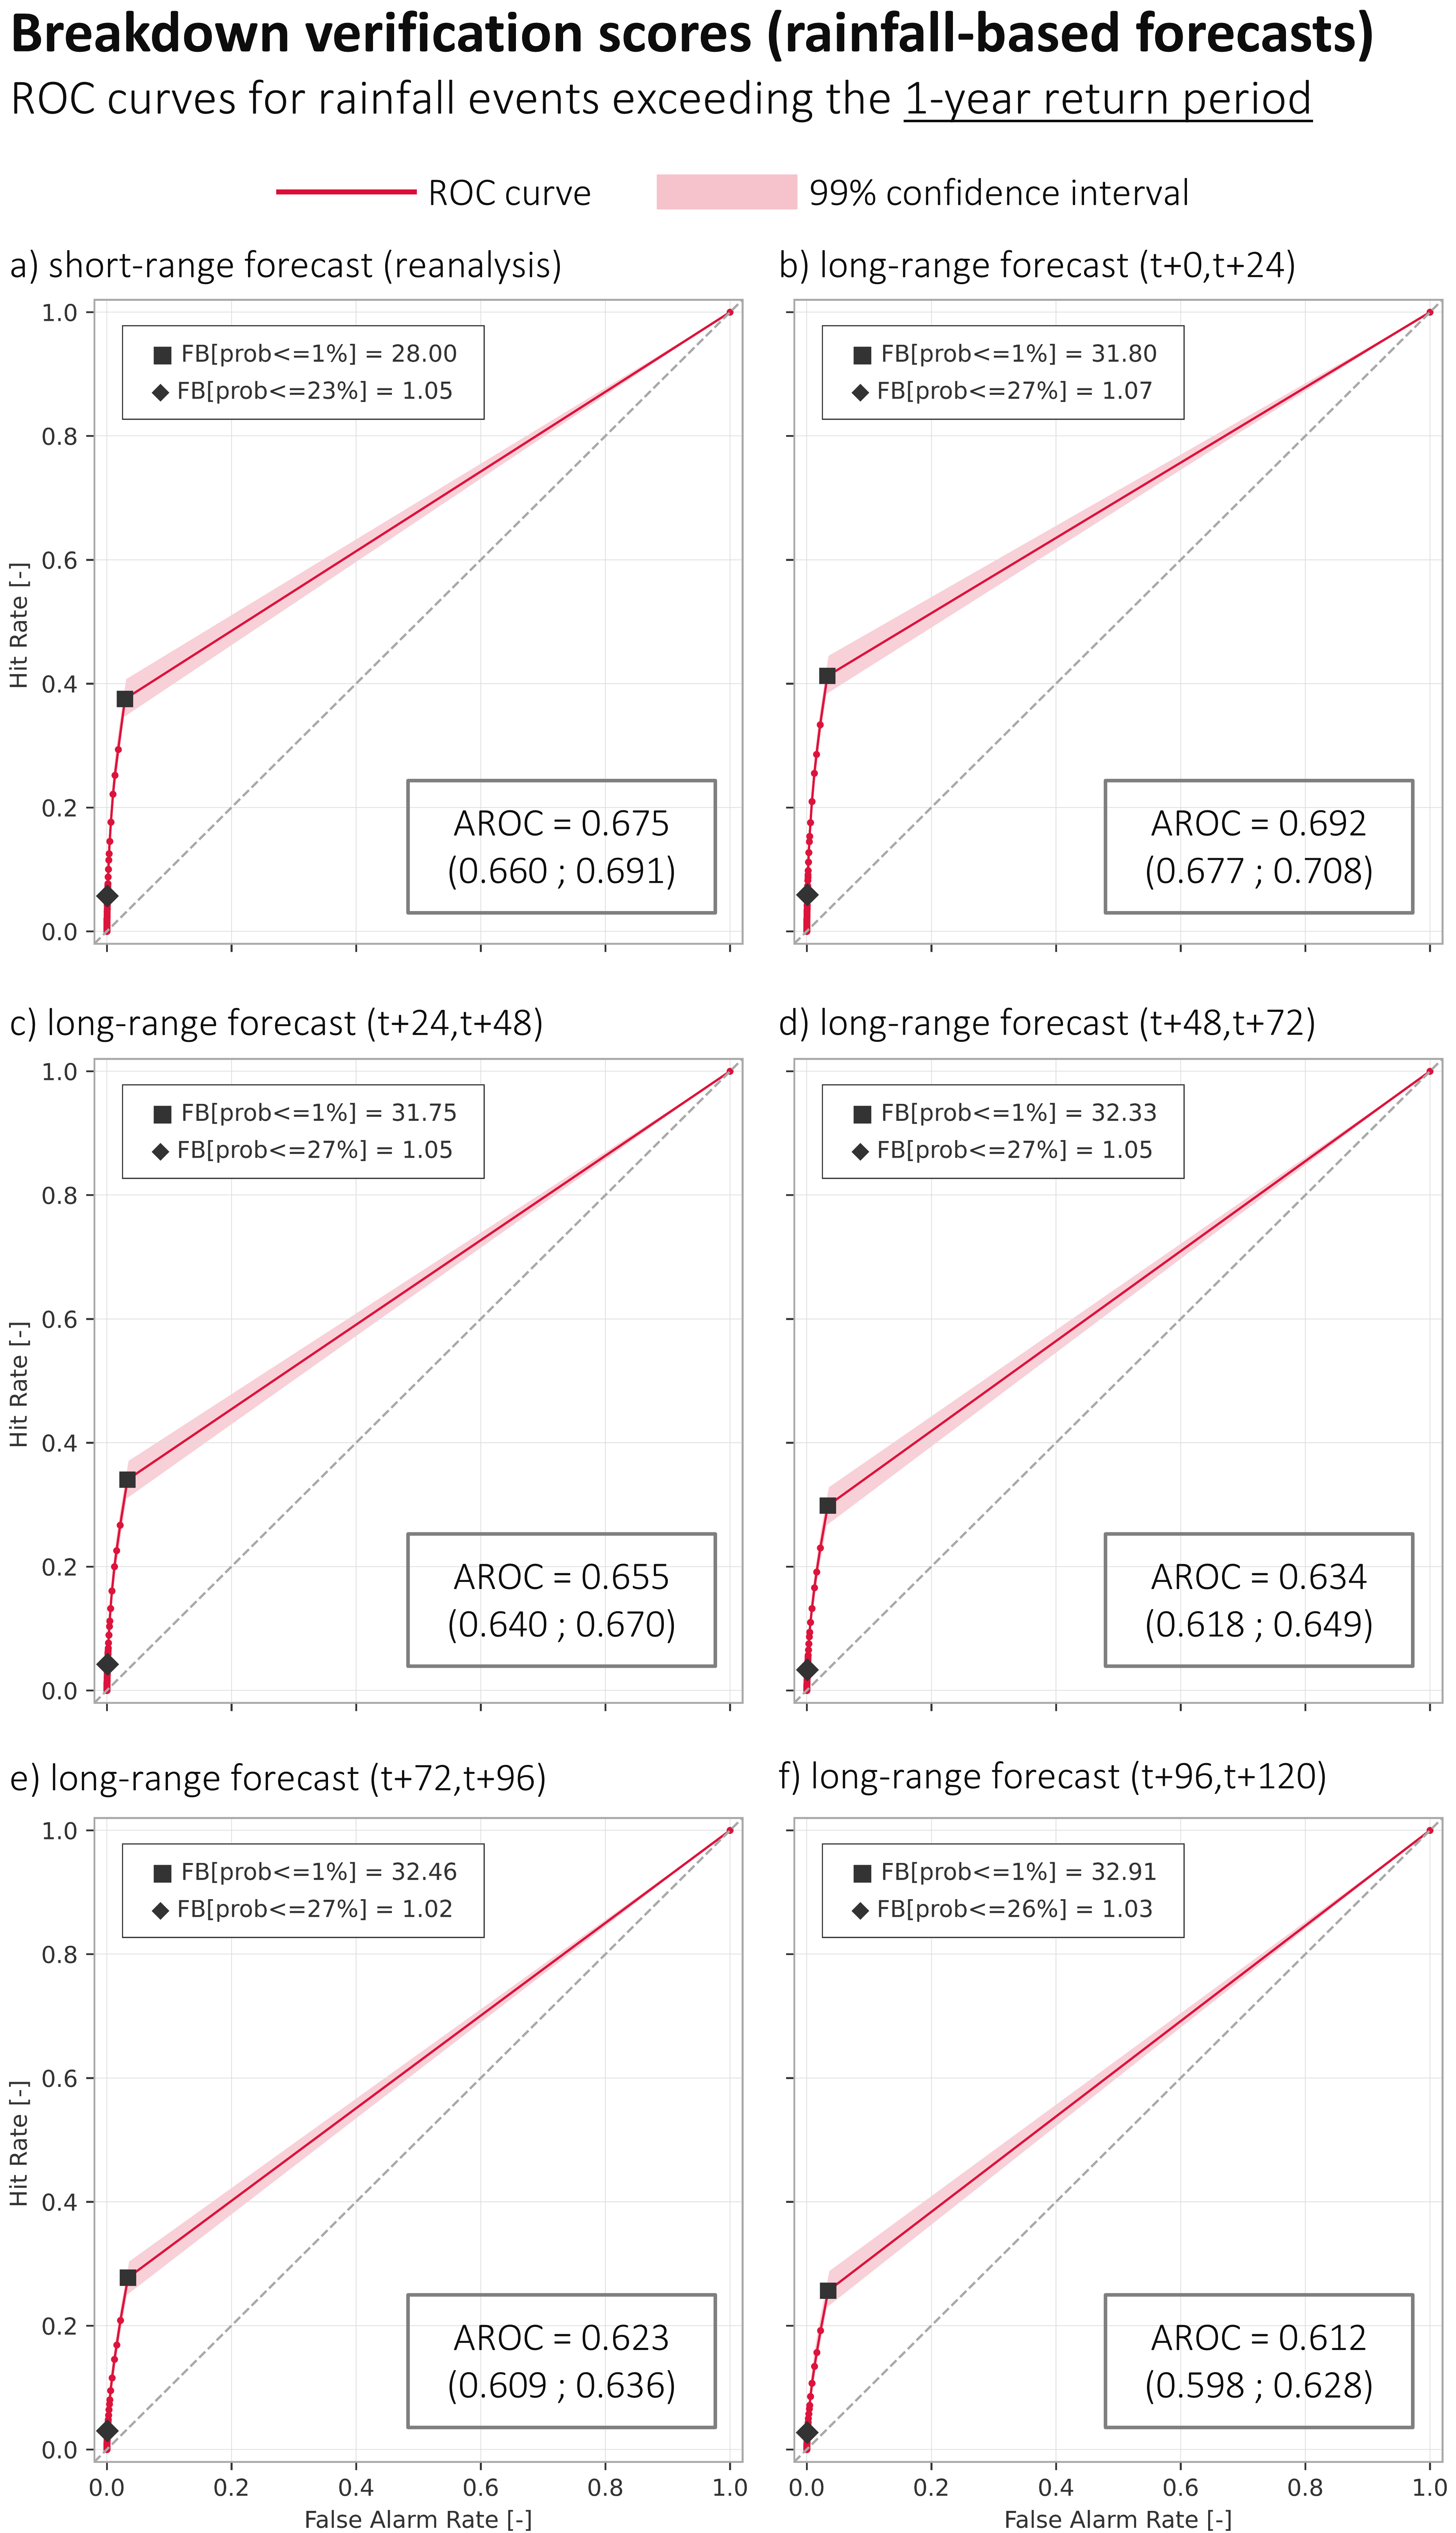
\includegraphics[width=\textwidth]{chapter_05/figures/rainfall_based_ff_verif_breakdown_scores_roc_1rp.png}
\caption{\textbf{ROC curves for tp >= 1-year return period for the rainfall-based forecasts of areas at risk of flash floods built with ERA5-ecPoint.} Panel (a) shows the ROC curve (blue solid line) for the short-range predictions together with the confidence intervals (blue shaded area) at 99\% confidence level. Panels (b) to (f) refer to the long-range forecasts, for accumulation periods ending in t+24, t+48, t+72, t+96, and t+120, respectively. The pink dots refer to the probability threshold at which the frequency bias has the closest value to 1 (i.e., perfectly reliable forecast), while the orange dot shows the value of the frequency bias for the lowest probability threshold available in ERA5-ecPoint (i.e., the 99th percentile).}
\label{fig:rainfall_based_ff_verif_breakdown_scores_roc_1rp}
\end{figure}

The pink dot in Figure \ref{fig:rainfall_based_ff_verif_breakdown_scores_roc_1rp}a shows that perfect reliability (i.e. frequency bias equal to 1) is reach for probabilities <= 23\%. For the long-range forecasts, the probability thresholds at which perfect reliability is achieved is compatible to the short-range, being 27\% for all the lead times except t+120 which is 26\%. The frequency bias for the lowest probability threshold (i.e. 99th percentile or probability threshold equal to 1\%) in the short-range forecasts equals to 28. The frequency biases for the long-range forecasts are similar, falling between 31 and 33. 

Similar results are obtained for the 5-, 10-, 20-, 50-, and 100-year return periods.

\begin{figure}[htbp]
\centering
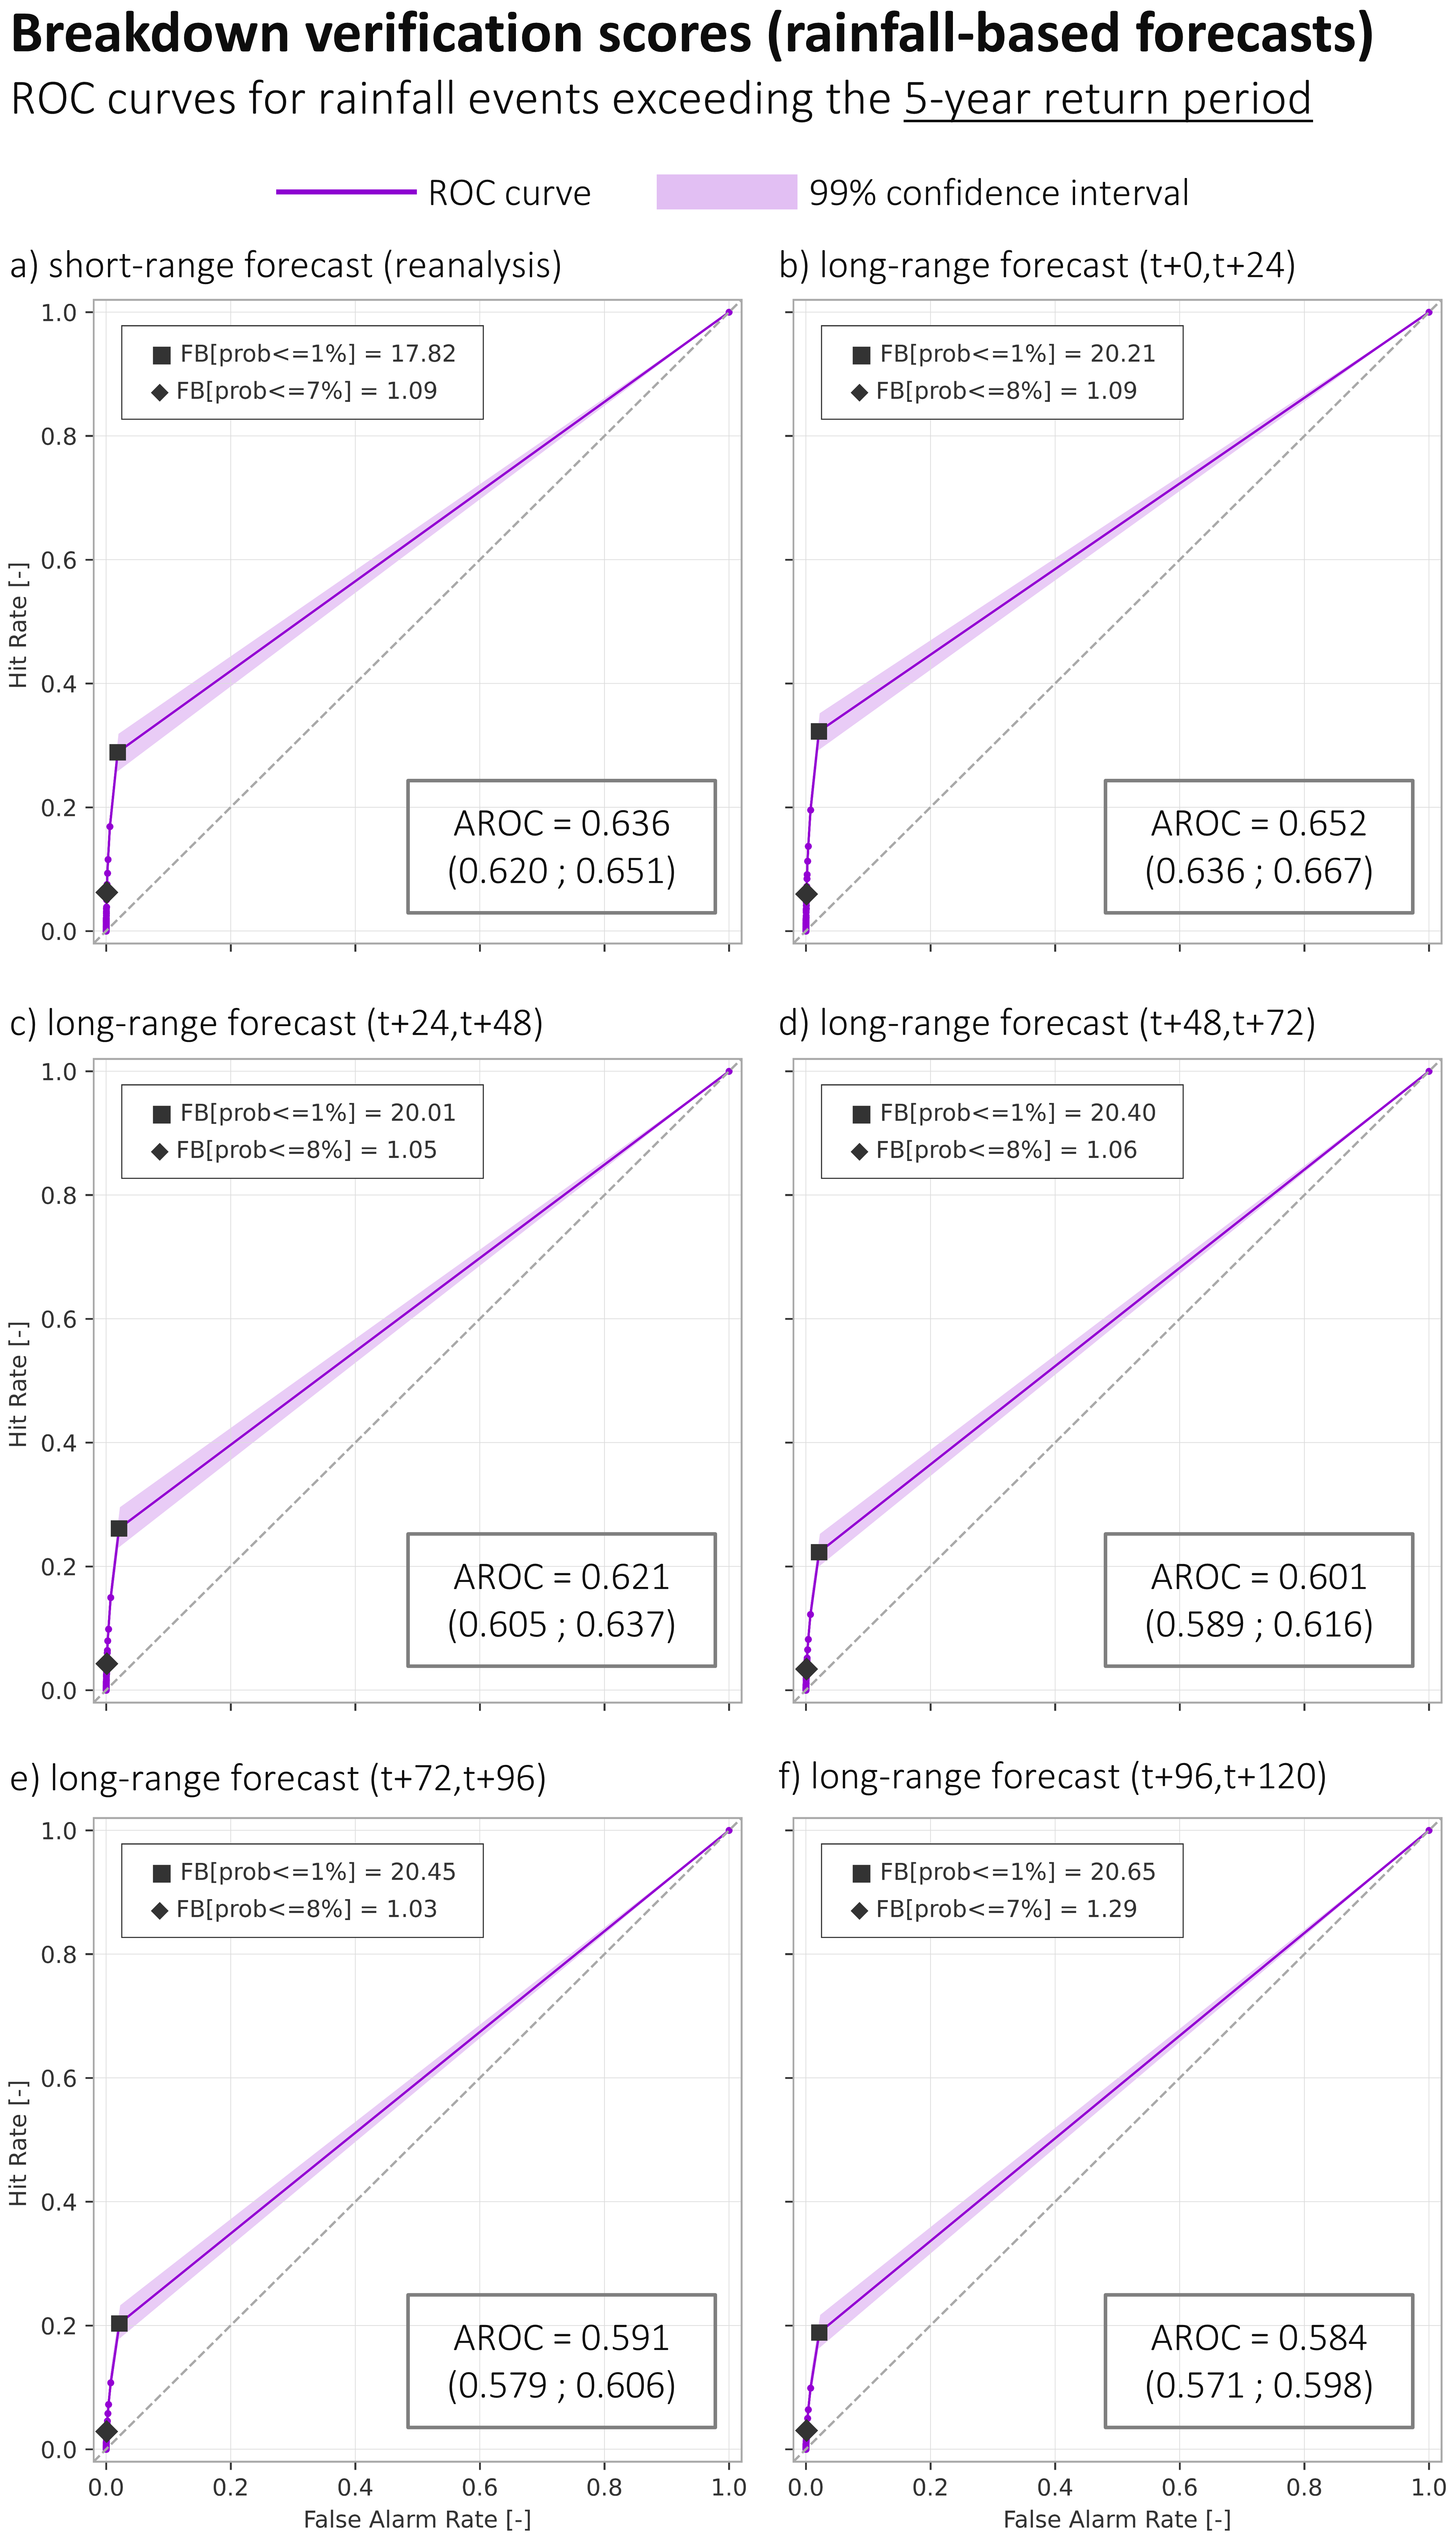
\includegraphics[width=\textwidth]{chapter_05/figures/rainfall_based_ff_verif_breakdown_scores_roc_5rp.png}
\caption{\textbf{ROC curves for tp >= 5-year return period for the rainfall-based forecasts of areas at risk of flash floods built with ERA5-ecPoint.} Similar to Figure \ref{fig:rainfall_based_ff_verif_breakdown_scores_roc_1rp}.}
\label{fig:rainfall_based_ff_verif_breakdown_scores_roc_5rp}
\end{figure}

\begin{figure}[htbp]
\centering
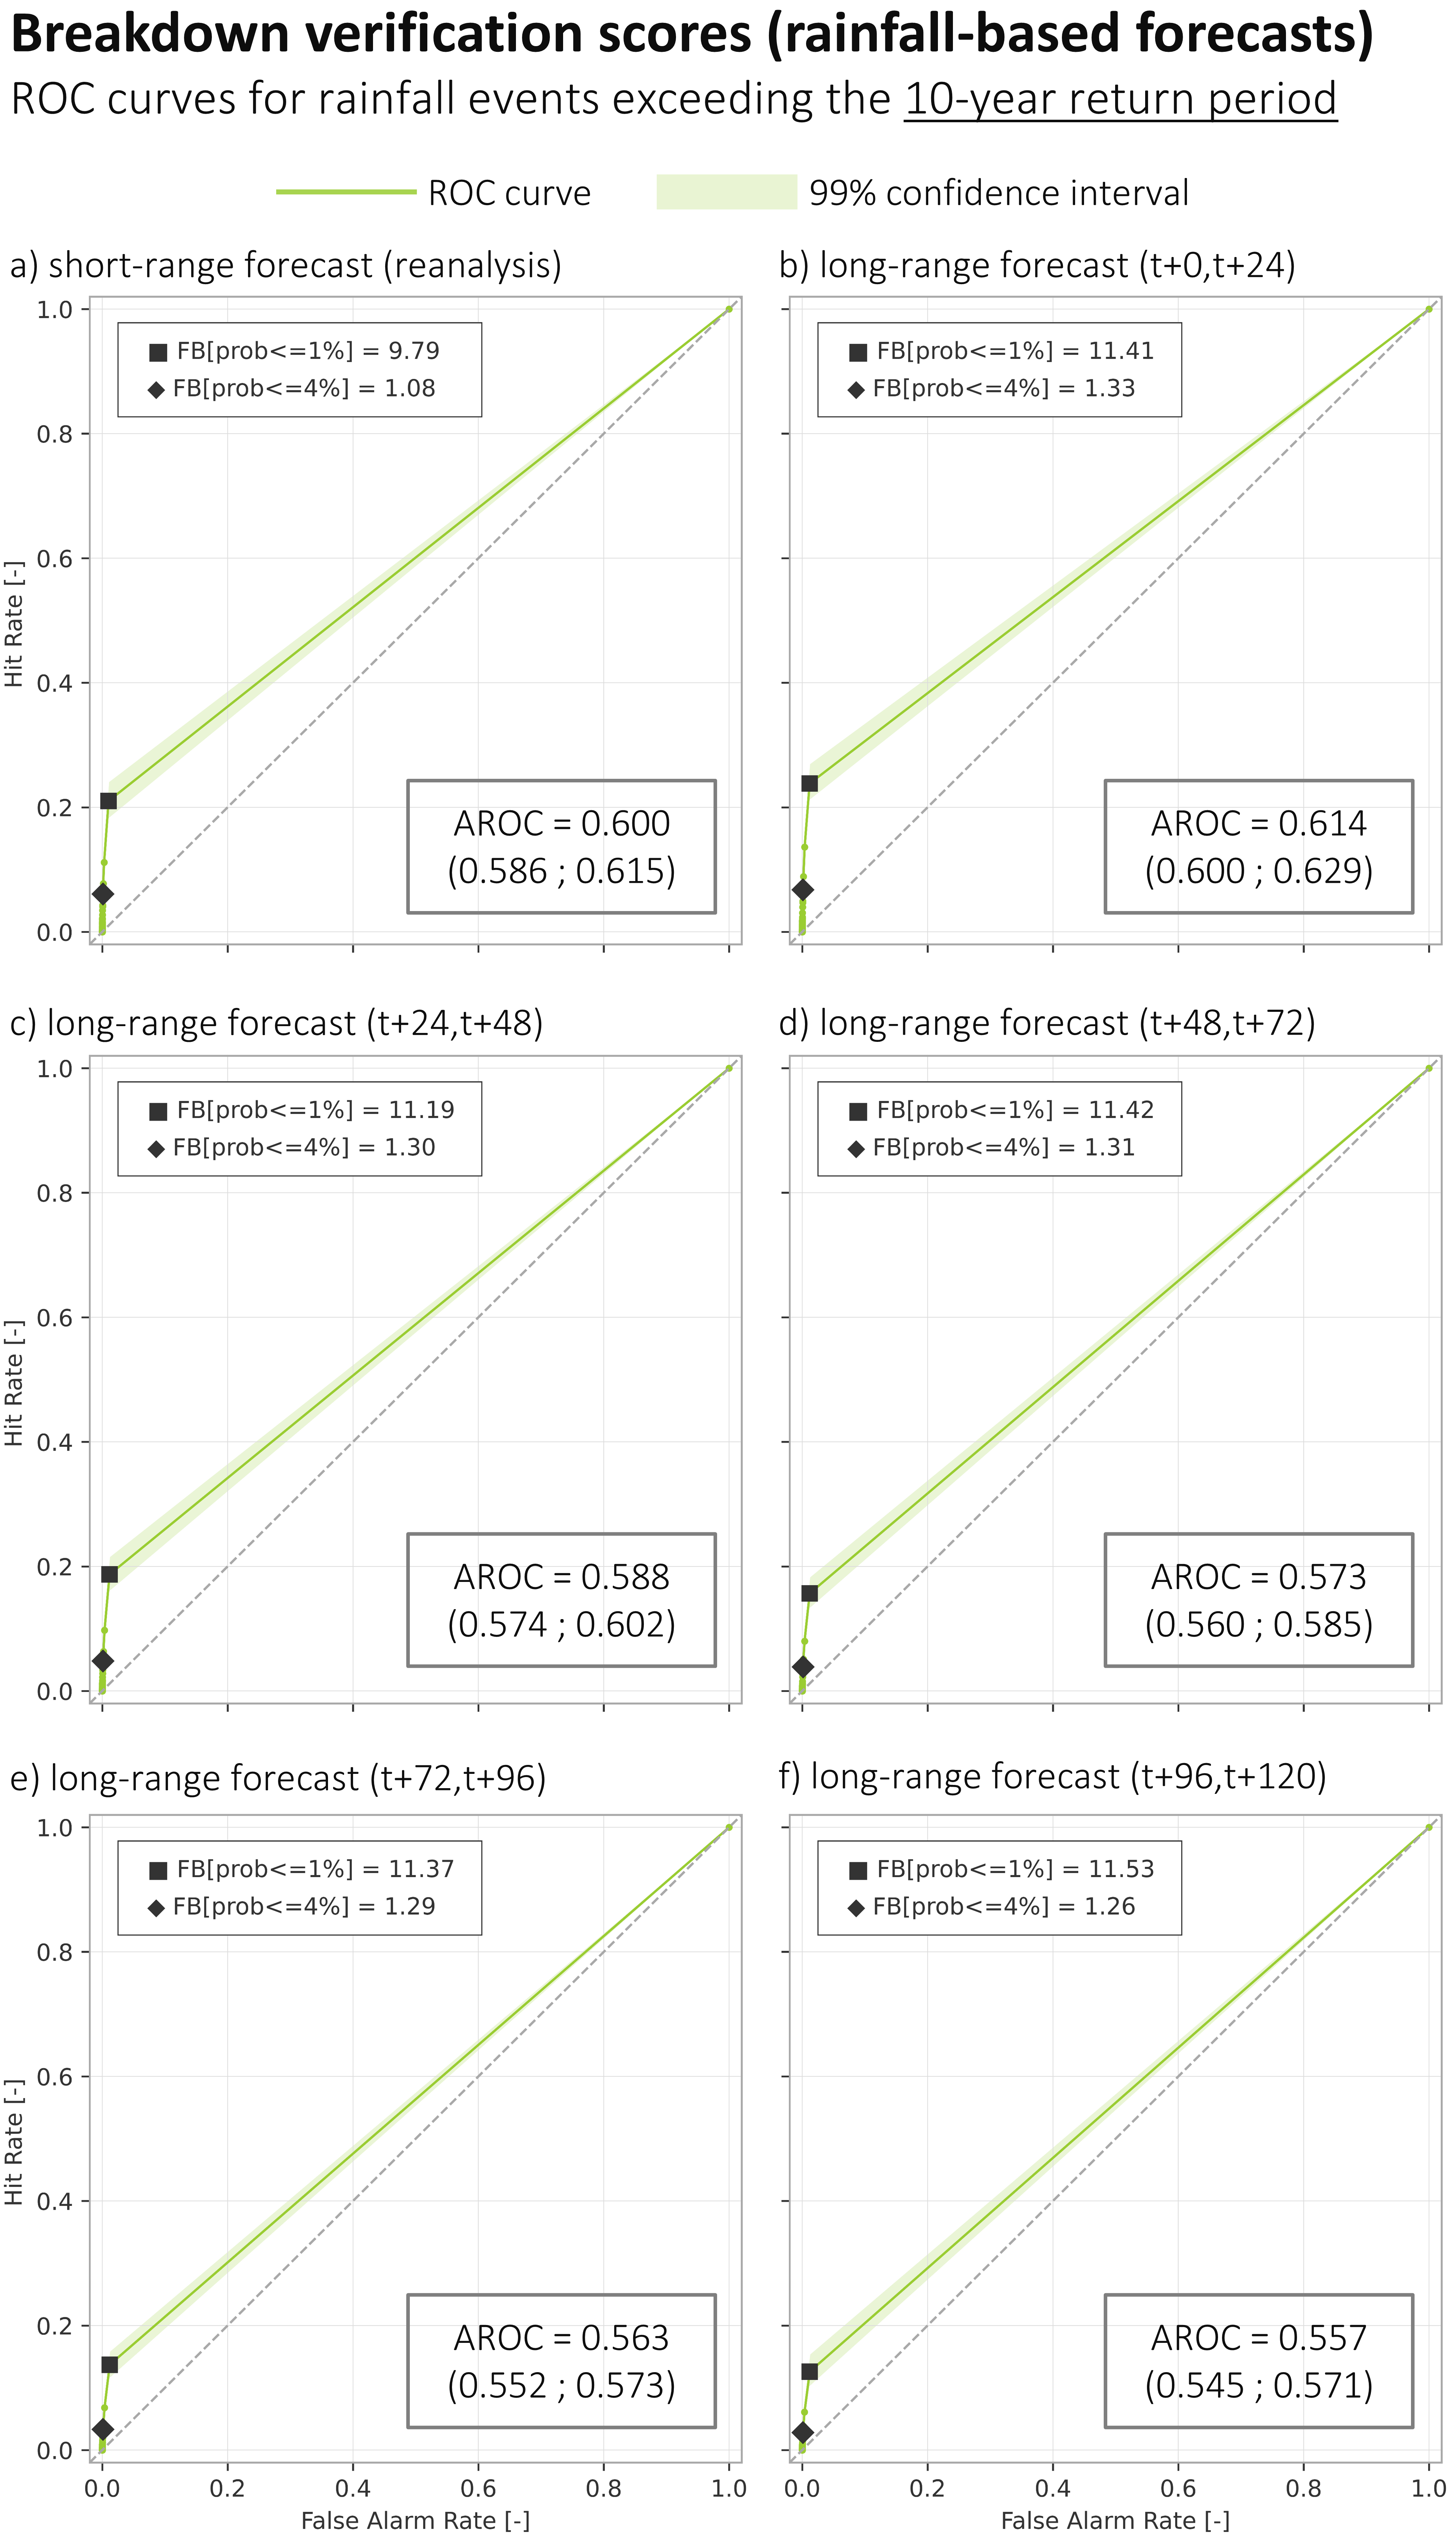
\includegraphics[width=\textwidth]{chapter_05/figures/rainfall_based_ff_verif_breakdown_scores_roc_10rp.png}
\caption{\textbf{ROC curves for tp >= 10-year return period for the rainfall-based forecasts of areas at risk of flash floods built with ERA5-ecPoint.} Similar to Figure \ref{fig:rainfall_based_ff_verif_breakdown_scores_roc_1rp}.}
\label{fig:rainfall_based_ff_verif_breakdown_scores_roc_10rp}
\end{figure}

\begin{figure}[htbp]
\centering
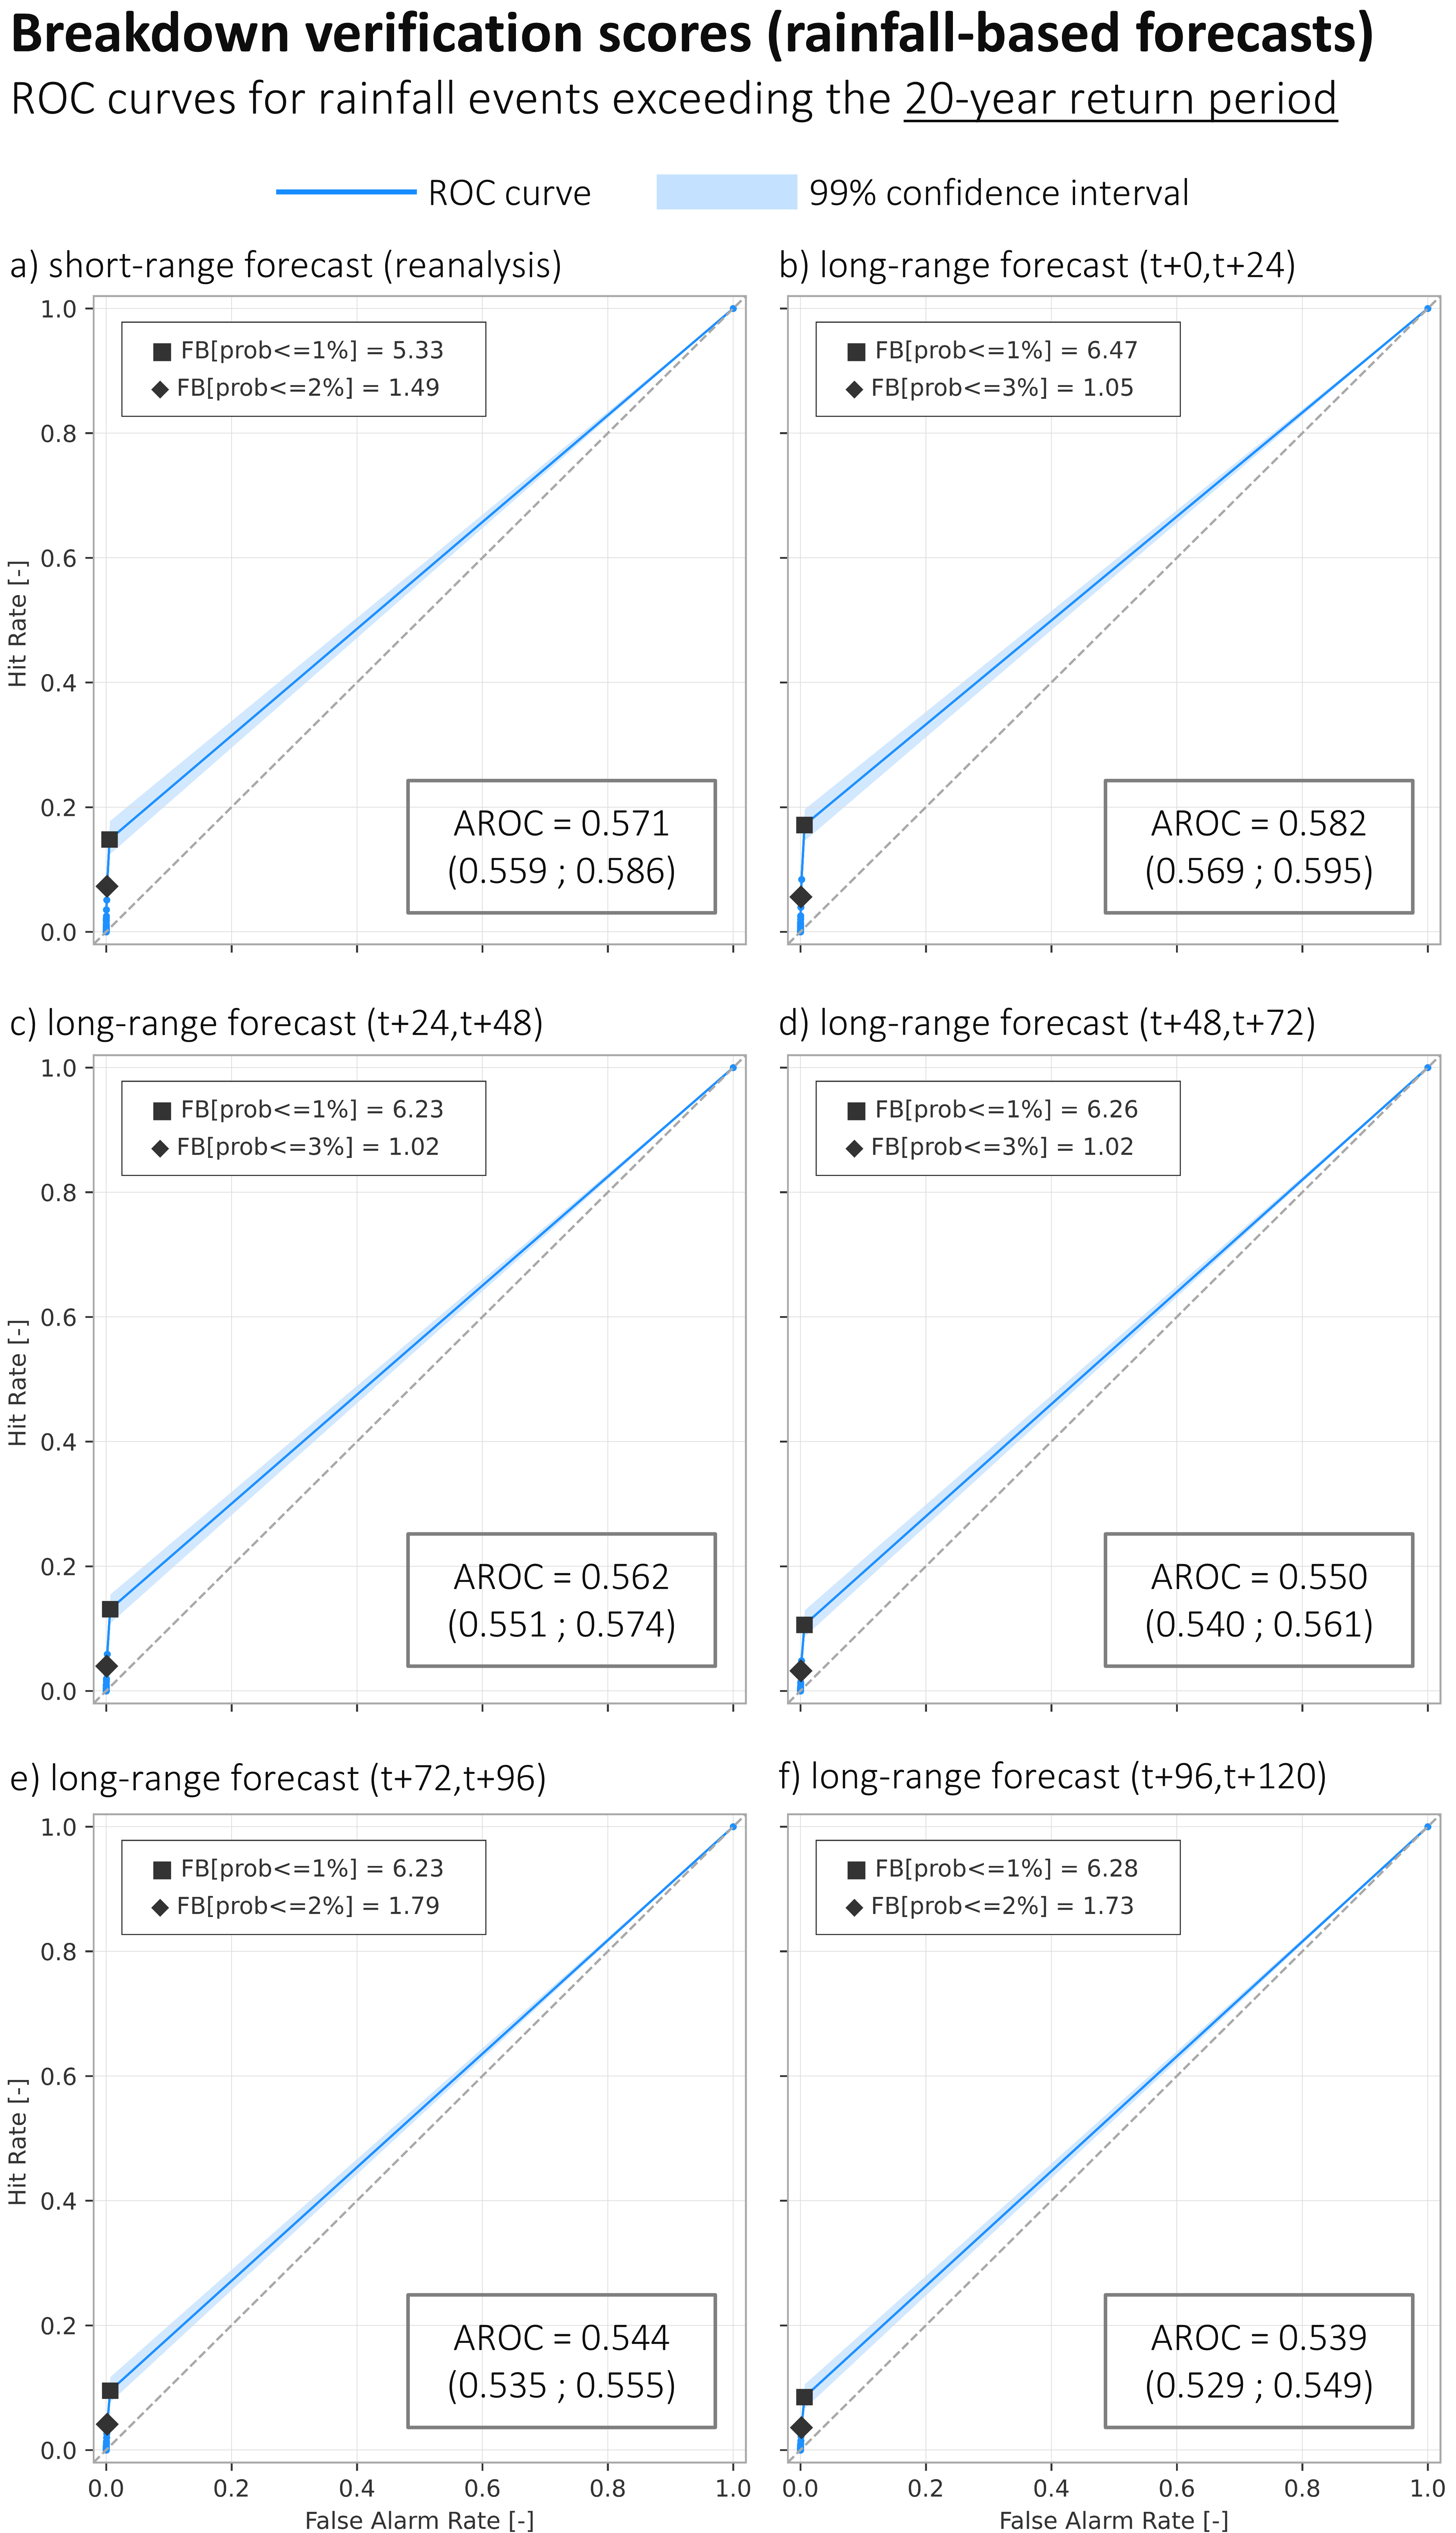
\includegraphics[width=\textwidth]{chapter_05/figures/rainfall_based_ff_verif_breakdown_scores_roc_20rp.png}
\caption{\textbf{ROC curves for tp >= 20-year return period for the rainfall-based forecasts of areas at risk of flash floods built with ERA5-ecPoint.} Similar to Figure \ref{fig:rainfall_based_ff_verif_breakdown_scores_roc_1rp}.}
\label{fig:rainfall_based_ff_verif_breakdown_scores_roc_20rp}
\end{figure}

\begin{figure}[htbp]
\centering
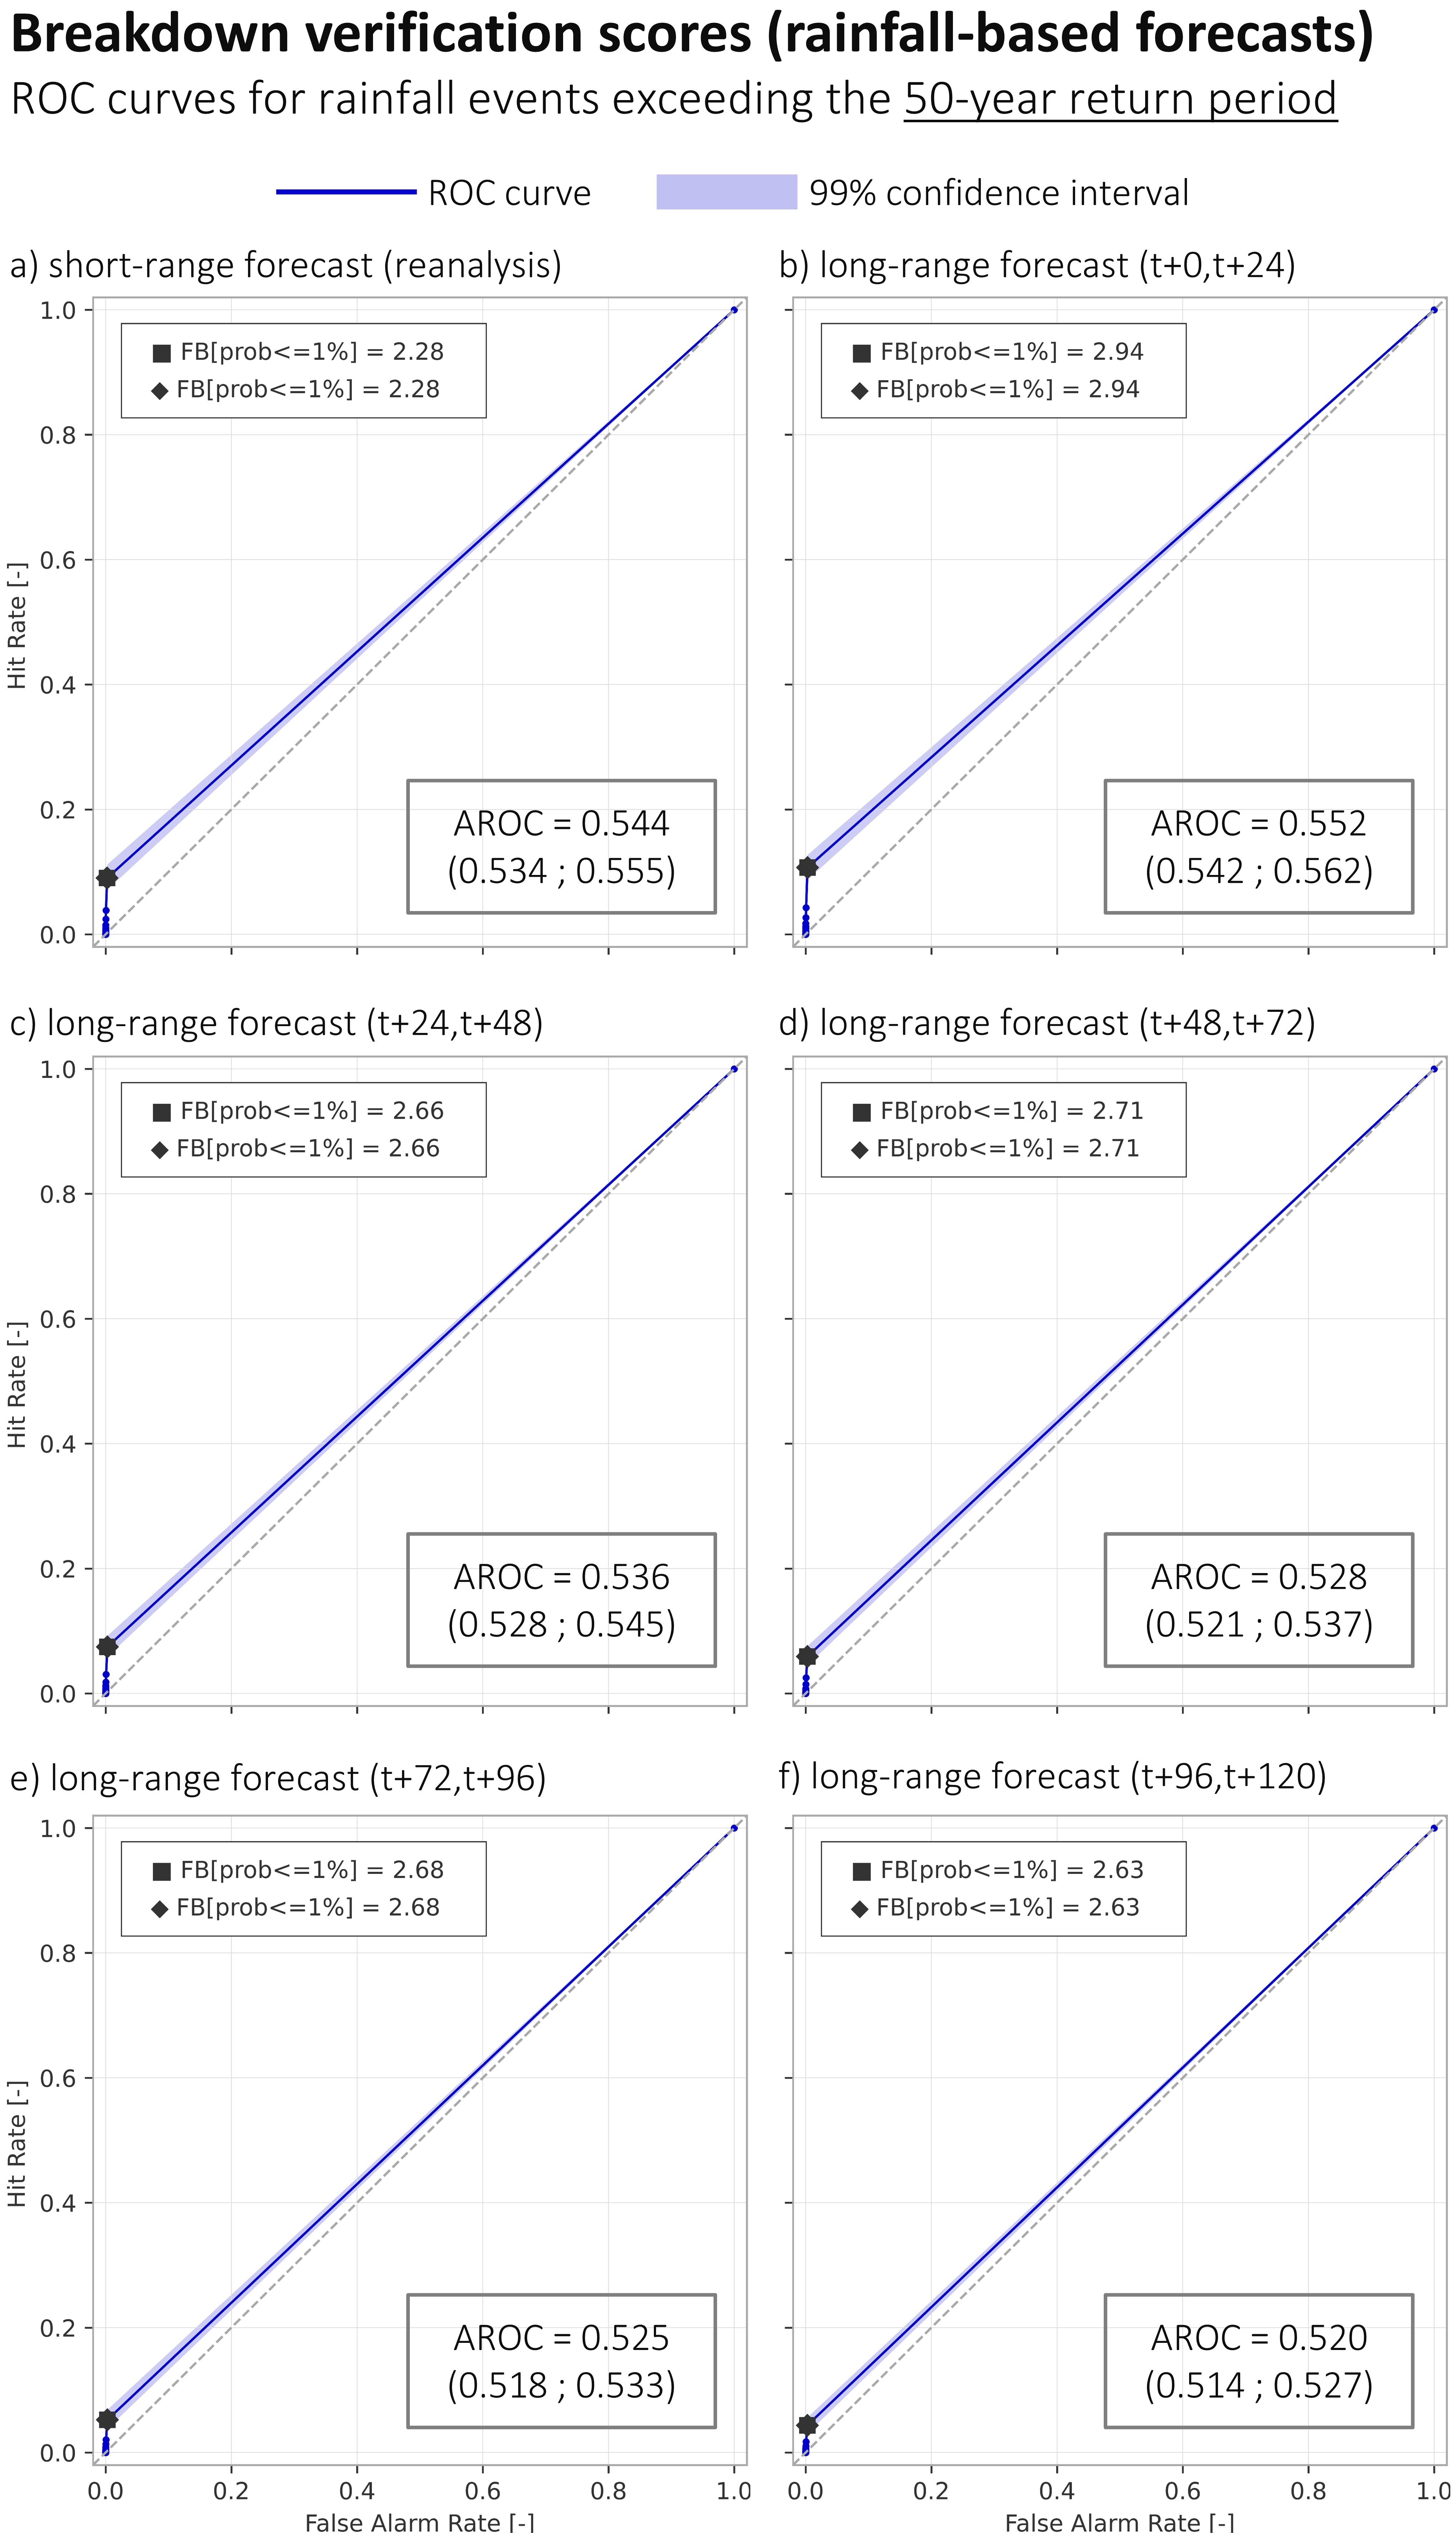
\includegraphics[width=\textwidth]{chapter_05/figures/rainfall_based_ff_verif_breakdown_scores_roc_50rp.png}
\caption{\textbf{ROC curves for tp >= 50-year return period for the rainfall-based forecasts of areas at risk of flash floods built with ERA5-ecPoint.} Similar to Figure \ref{fig:rainfall_based_ff_verif_breakdown_scores_roc_1rp}.}
\label{fig:rainfall_based_ff_verif_breakdown_scores_roc_50rp}
\end{figure}

\begin{figure}[htbp]
\centering
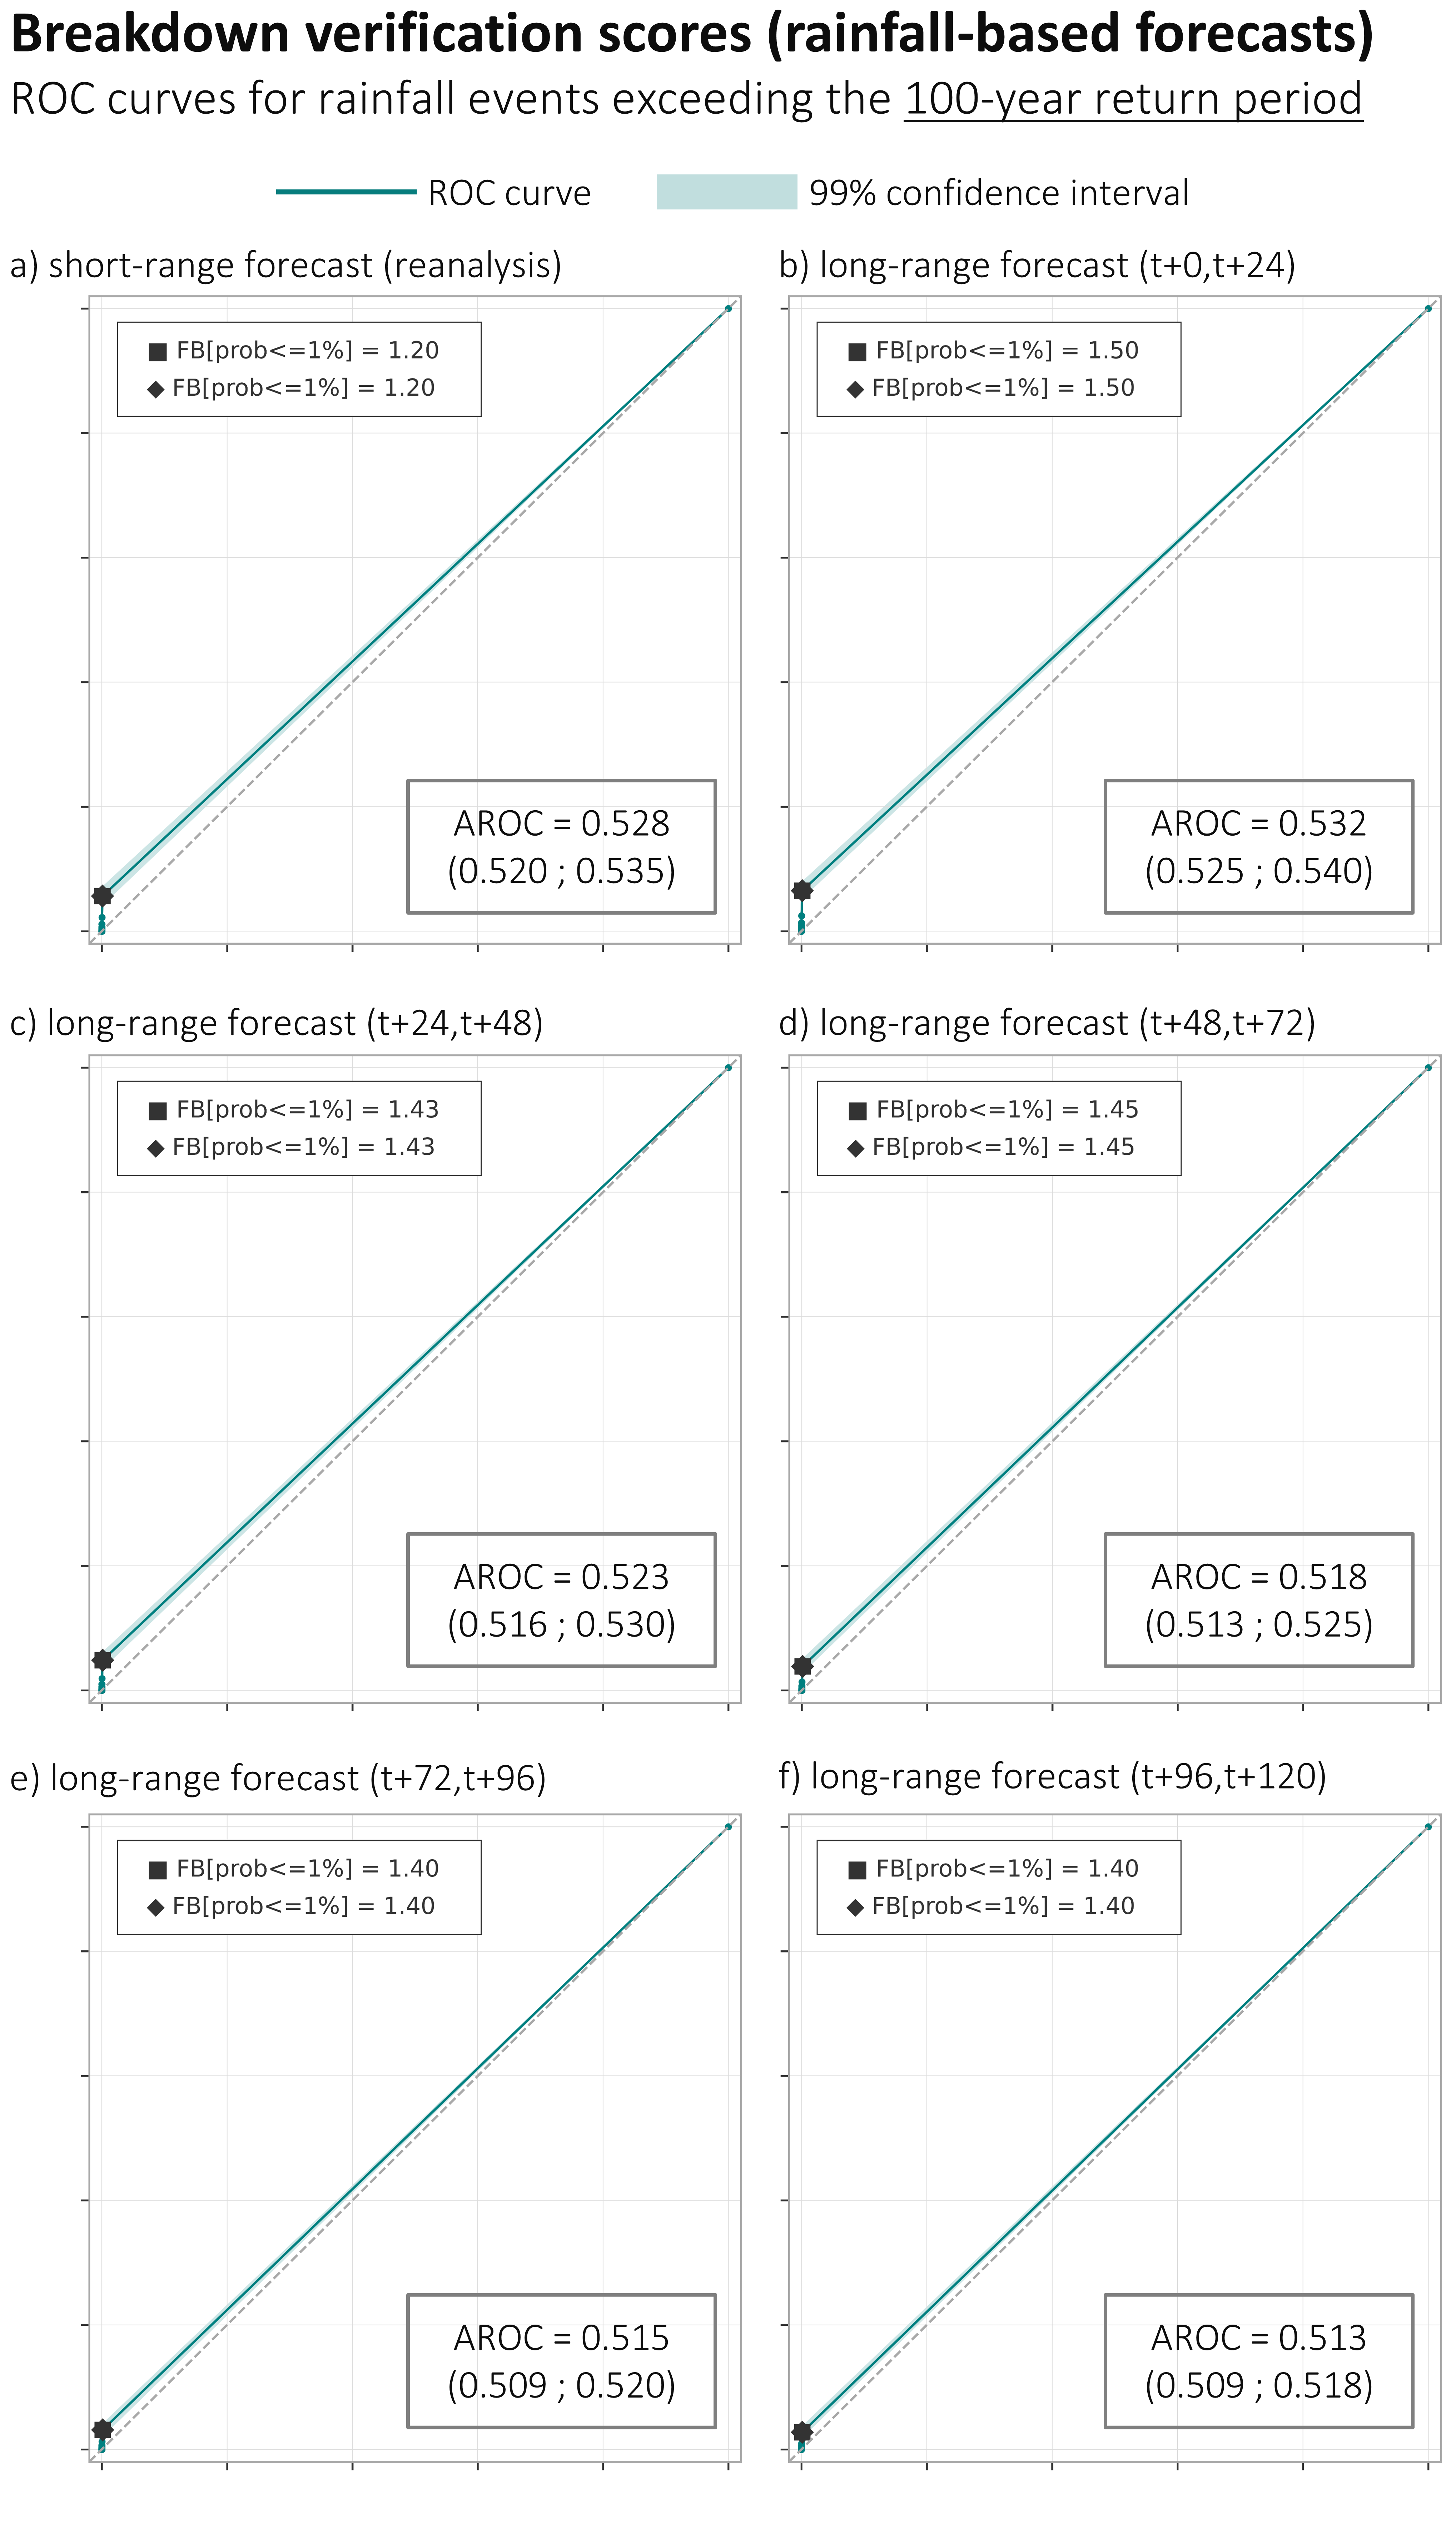
\includegraphics[width=\textwidth]{chapter_05/figures/rainfall_based_ff_verif_breakdown_scores_roc_100rp.png}
\caption{\textbf{ROC curves for tp >= 100-year return period for the rainfall-based forecasts of areas at risk of flash floods built with ERA5-ecPoint.} Similar to Figure \ref{fig:rainfall_based_ff_verif_breakdown_scores_roc_1rp}.}
\label{fig:rainfall_based_ff_verif_breakdown_scores_roc_100rp}
\end{figure}


\subsection{Reliability}

All forecasts for rainfall events exceeding the 1-year return period threshold (Figure \ref{fig:rainfall_based_ff_verif_breakdown_scores_rel_diag_1rp}) exhibit a systematic overprediction across all lead times, as shown by the reliability diagram being below the diagonal line. This indicates that when the model predicts a given probability, the observed frequency of flash flood events is consistently lower. For example, when the forecasts indicate a 50\% chance of having a flash flood event, the observed frequency ranges from \sim10\% in the short-range forecasts (Figure \ref{fig:rainfall_based_ff_verif_breakdown_scores_rel_diag_1rp}a), and between 10\% (for t+24, Figure \ref{fig:rainfall_based_ff_verif_breakdown_scores_rel_diag_1rp}b) and 2\% (t+120, Figure \ref{fig:rainfall_based_ff_verif_breakdown_scores_rel_diag_1rp}f) in the long-range forecasts. As seen in the ROC curves, the confidence intervals at 99\% are fairly narrow, suggesting that the differences between the reliability diagrams at different lead times are significant at the considered confidence level. However, the confidence levels increase with increasing forecast probabilities. As seen in the corresponding sharpness diagrams (inset boxes in all panels of Figure \ref{fig:rainfall_based_ff_verif_breakdown_scores_rel_diag_1rp}), such widening of the confidence intervals is likely due to the low number of forecasts issued with probabilities higher than ~25\% (when the total number of instances lies below 1000 samples). Such predominance of low probability forecasts suggests that the model (ERA5-ecPoint) rarely expresses high confidence in extreme event occurrence. A notable characteristic of all the reliability diagrams in the Figure \ref{fig:rainfall_based_ff_verif_breakdown_scores_rel_diag_1rp} is the sharp increase in observed frequency for the highest probability bins (i.e. 80\% to 100\%). This steep rise suggests that when the model does issue high probability forecasts, these correspond to genuinely extreme events, though such forecasts remain infrequent.

\begin{figure}[htbp]
\centering
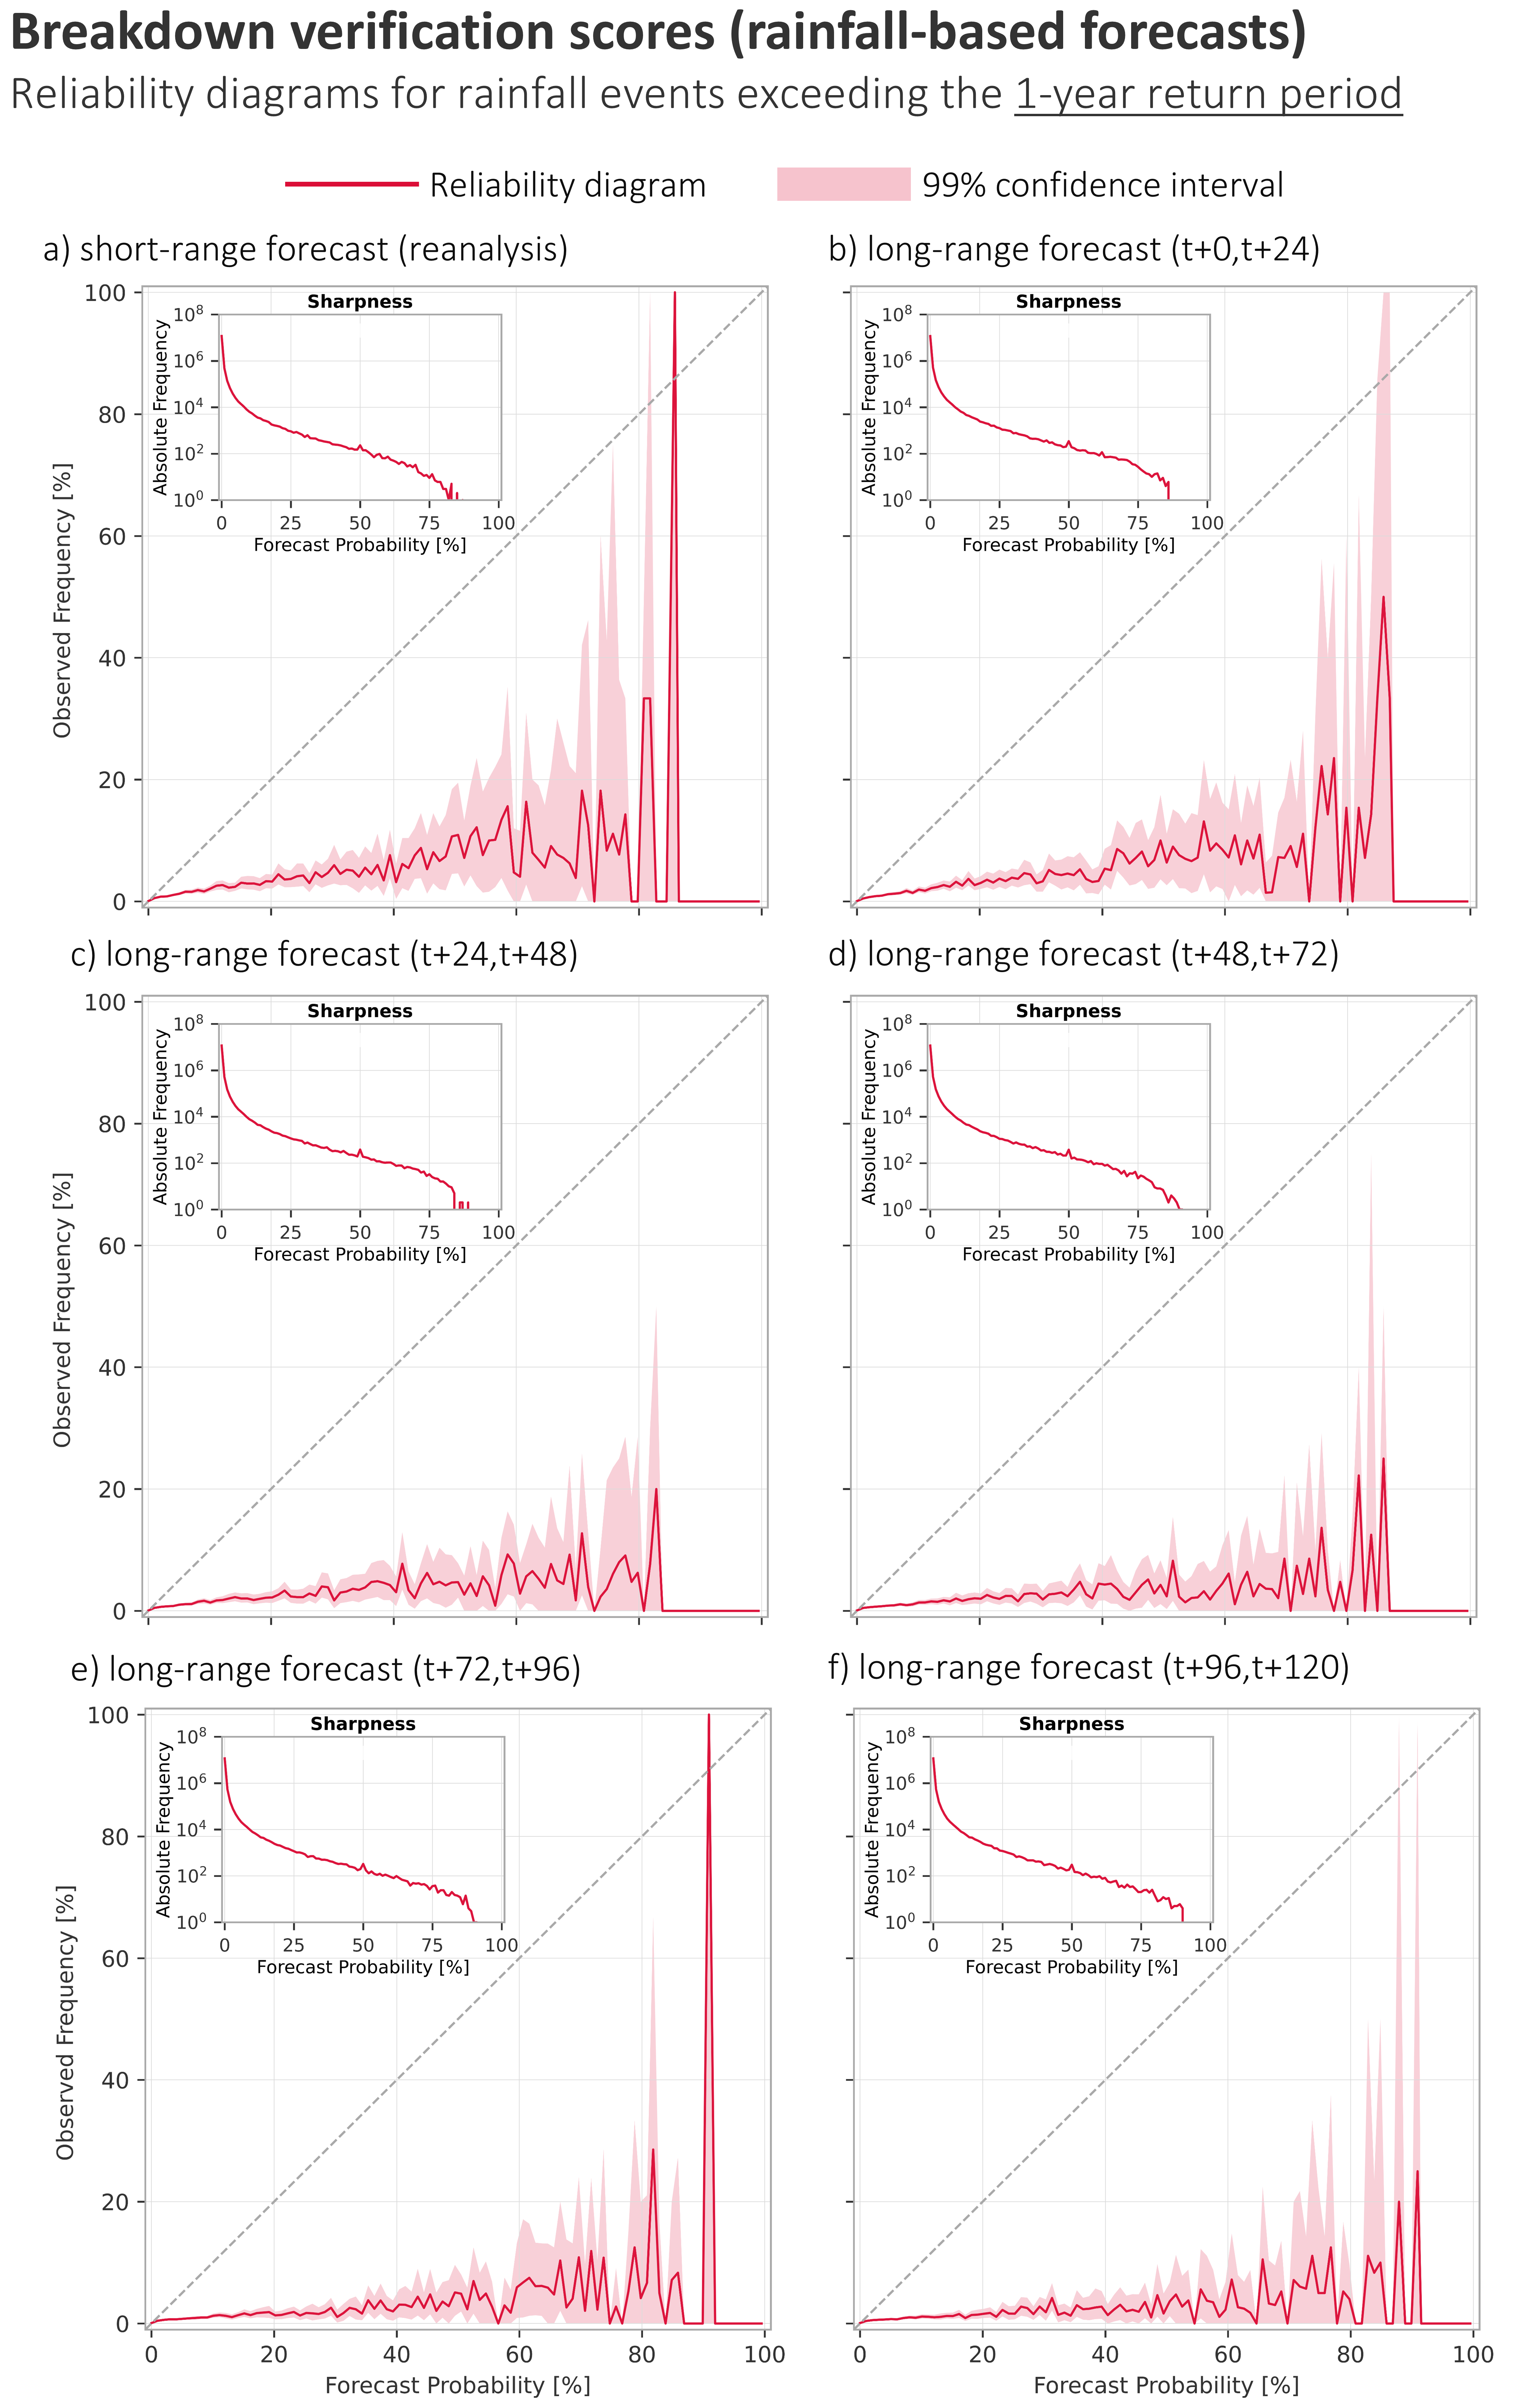
\includegraphics[width=\textwidth]{rainfall_based_ff_verif_breakdown_scores_rel_diag_1rp.png}
\caption{\textbf{Reliability diagrams for tp >= 1-year return period for the rainfall-based forecasts of areas at risk of flash floods built with ERA5-ecPoint.} Panel (a) shows the reliability diagram (blue solid line) for the short-range predictions together with the confidence intervals (blue shaded area) at 99\% confidence level. Panels (b) to (f) refer to the long-range forecasts for accumulation periods ending in t+24, t+48, t+72, t+96, and t+120, respectively. The inset boxes show the corresponding sharpness diagrams.}
\label{fig:rainfall_based_ff_verif_breakdown_scores_rel_diag_1rp}
\end{figure}

The temporal evolution from Figure \ref{fig:rainfall_based_ff_verif_breakdown_scores_rel_diag_1rp}a to f reveals subtle changes in the forecasts' reliability characteristics with increasing lead time. Whilst the general pattern of overprediction persists, from day 2 forecasts (t+48) results more squashed into a flat line over very small observed frequencies, indicating that even though the model issues forecasts with high probabilities of exceeding the 1-year return period at longer lead times with a similar frequency of the short-range forecasts and the day 1 (t+24) long-range forecast, such forecasts do not necessarily correspond to an observed flash flood event.

The reliability diagrams get closer to the diagonal line (indicating perfect bias) as we increase the rainfall threshold to identify the flash flood events. Perfect reliability is observed for rainfall events exceeding the 10-, 20-year, and 50-year return period with probabilities below 5\% at day 1 forecast (t+24) for the 10-, 20-year return period, and 10\% for the 50-year return period.

\begin{figure}[htbp]
\centering
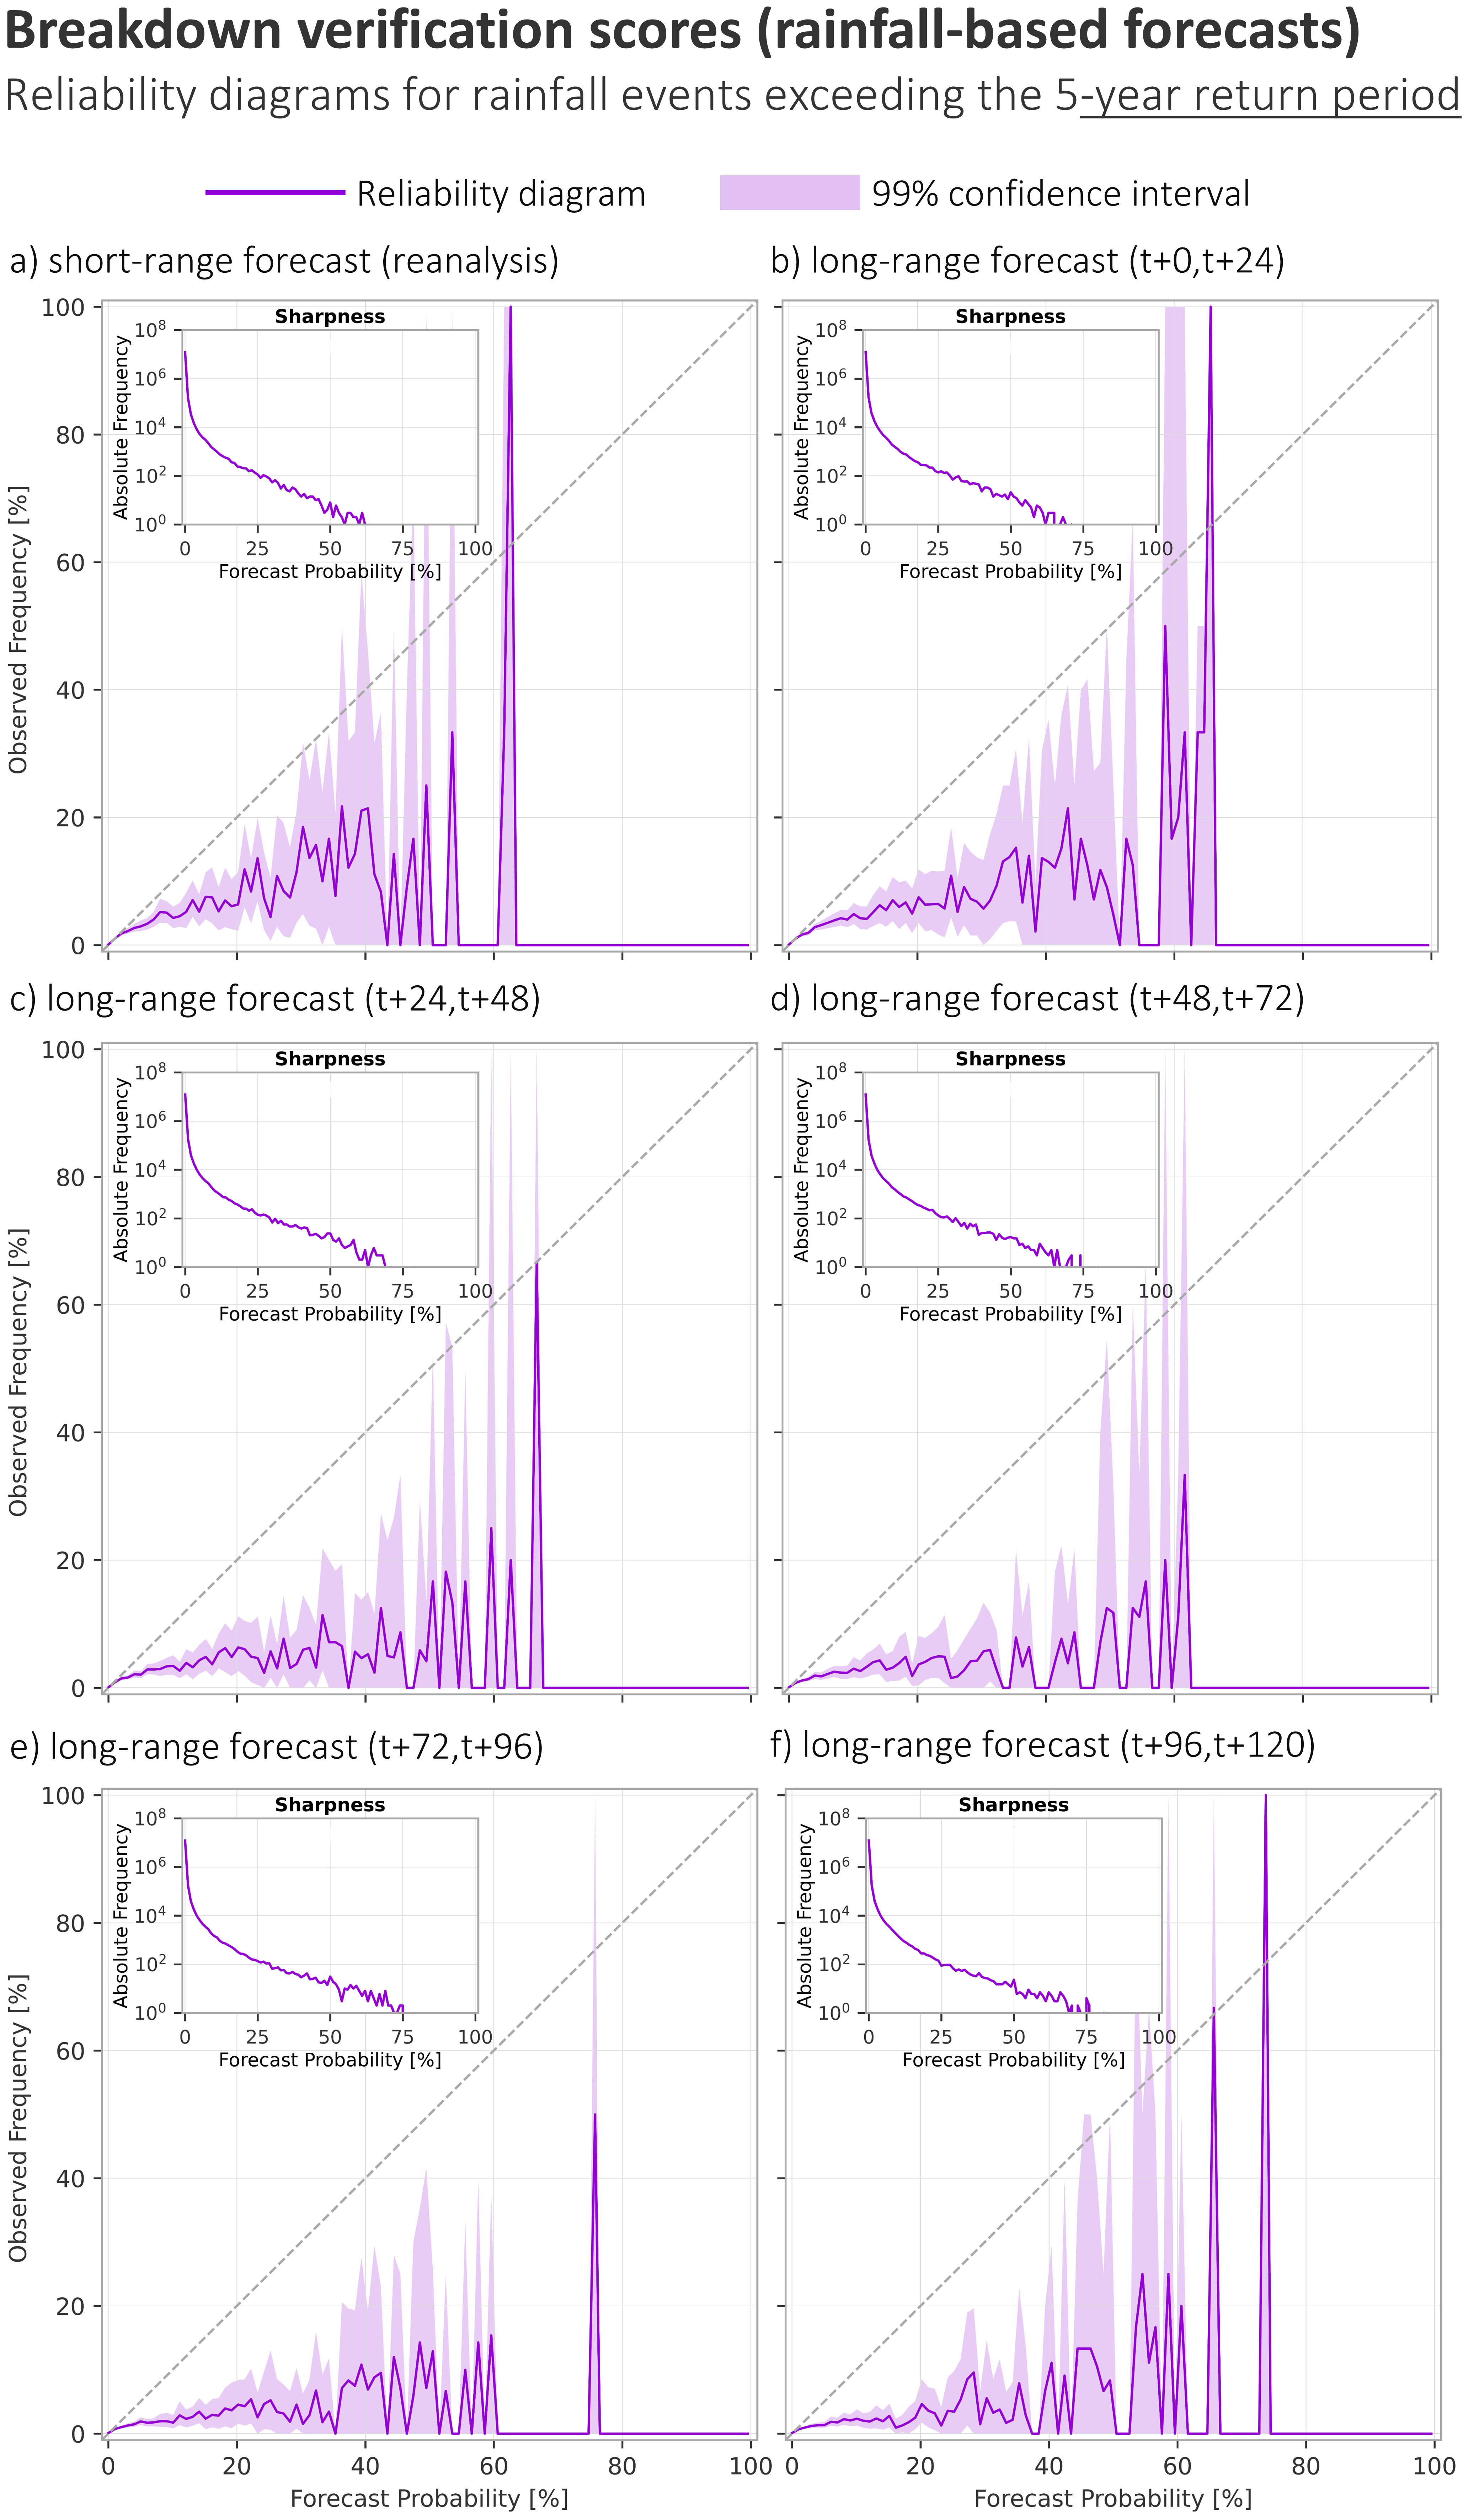
\includegraphics[width=\textwidth]{rainfall_based_ff_verif_breakdown_scores_rel_diag_5rp.png}
\caption{\textbf{Reliability diagrams for tp >= 5-year return period for the rainfall-based forecasts of areas at risk of flash floods built with ERA5-ecPoint.} Similar to Figure \ref{fig:rainfall_based_ff_verif_breakdown_scores_rel_diag_1rp}.}
\label{fig:rainfall_based_ff_verif_breakdown_scores_rel_diag_5rp}
\end{figure}

\begin{figure}[htbp]
\centering
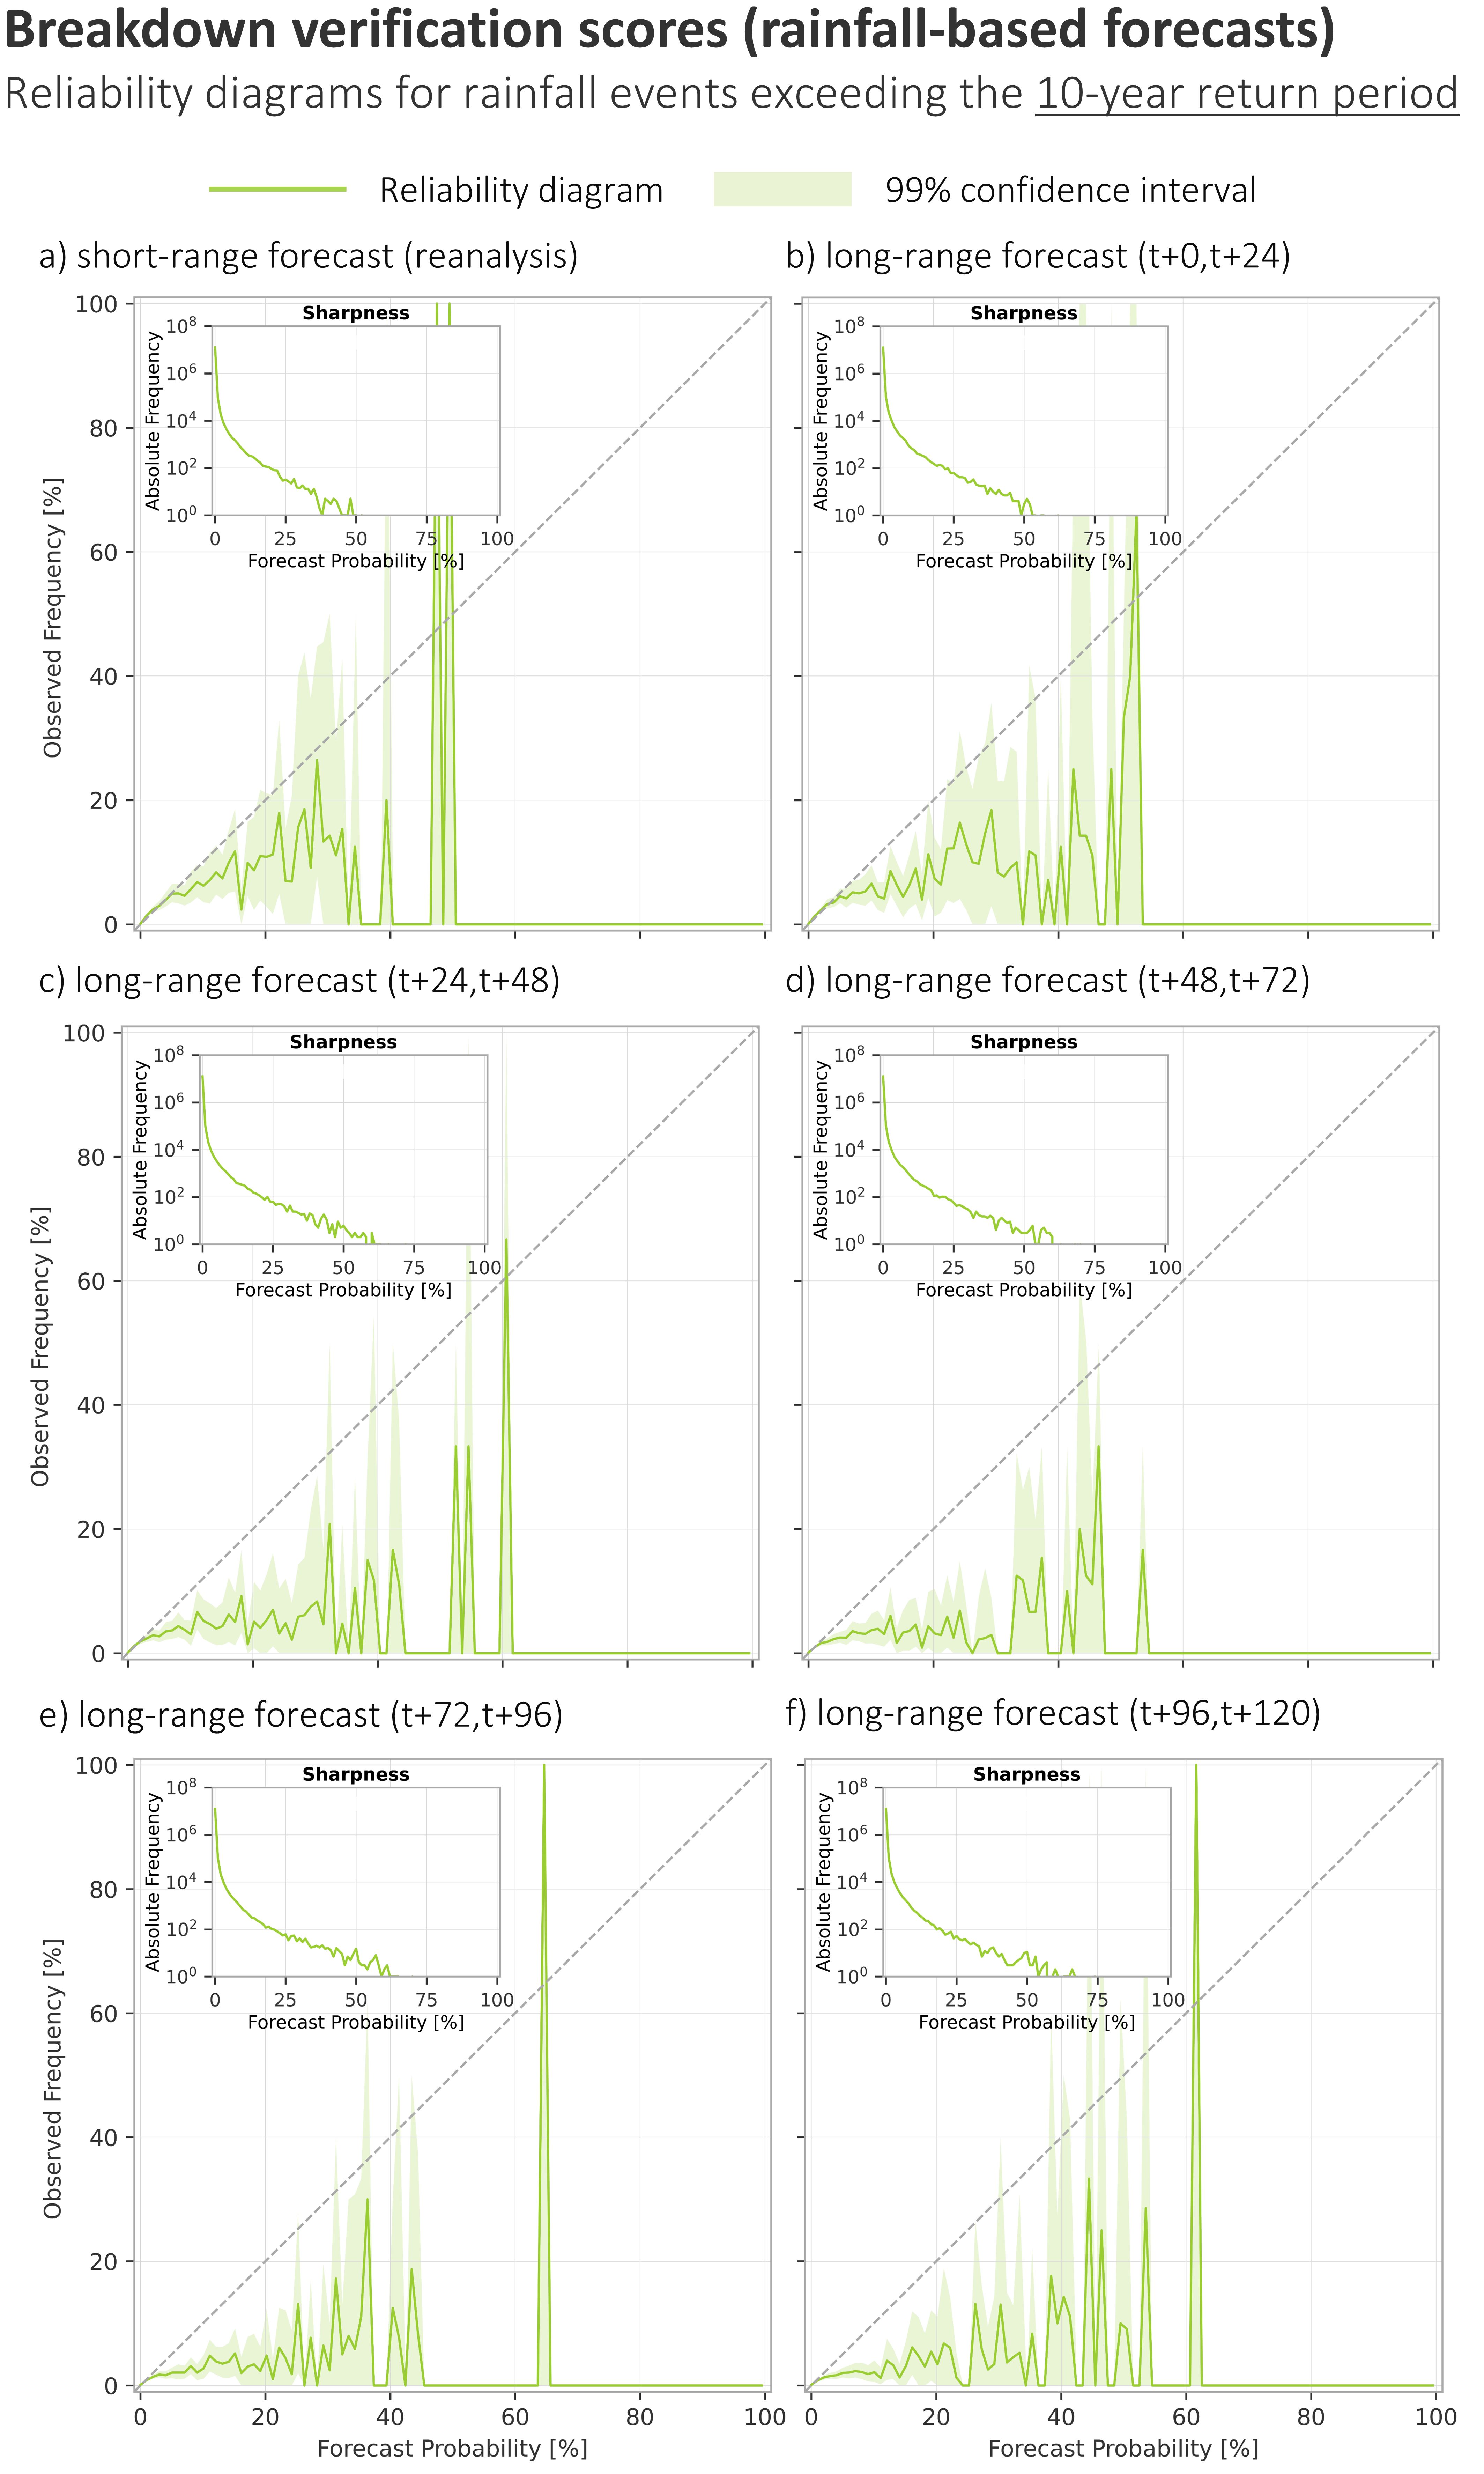
\includegraphics[width=\textwidth]{rainfall_based_ff_verif_breakdown_scores_rel_diag_10rp.png}
\caption{\textbf{Reliability diagrams for tp >= 5-year return period for the rainfall-based forecasts of areas at risk of flash floods built with ERA5-ecPoint.} Similar to Figure \ref{fig:rainfall_based_ff_verif_breakdown_scores_rel_diag_1rp}.}
\label{fig:rainfall_based_ff_verif_breakdown_scores_rel_diag_10rp}
\end{figure}

\begin{figure}[htbp]
\centering
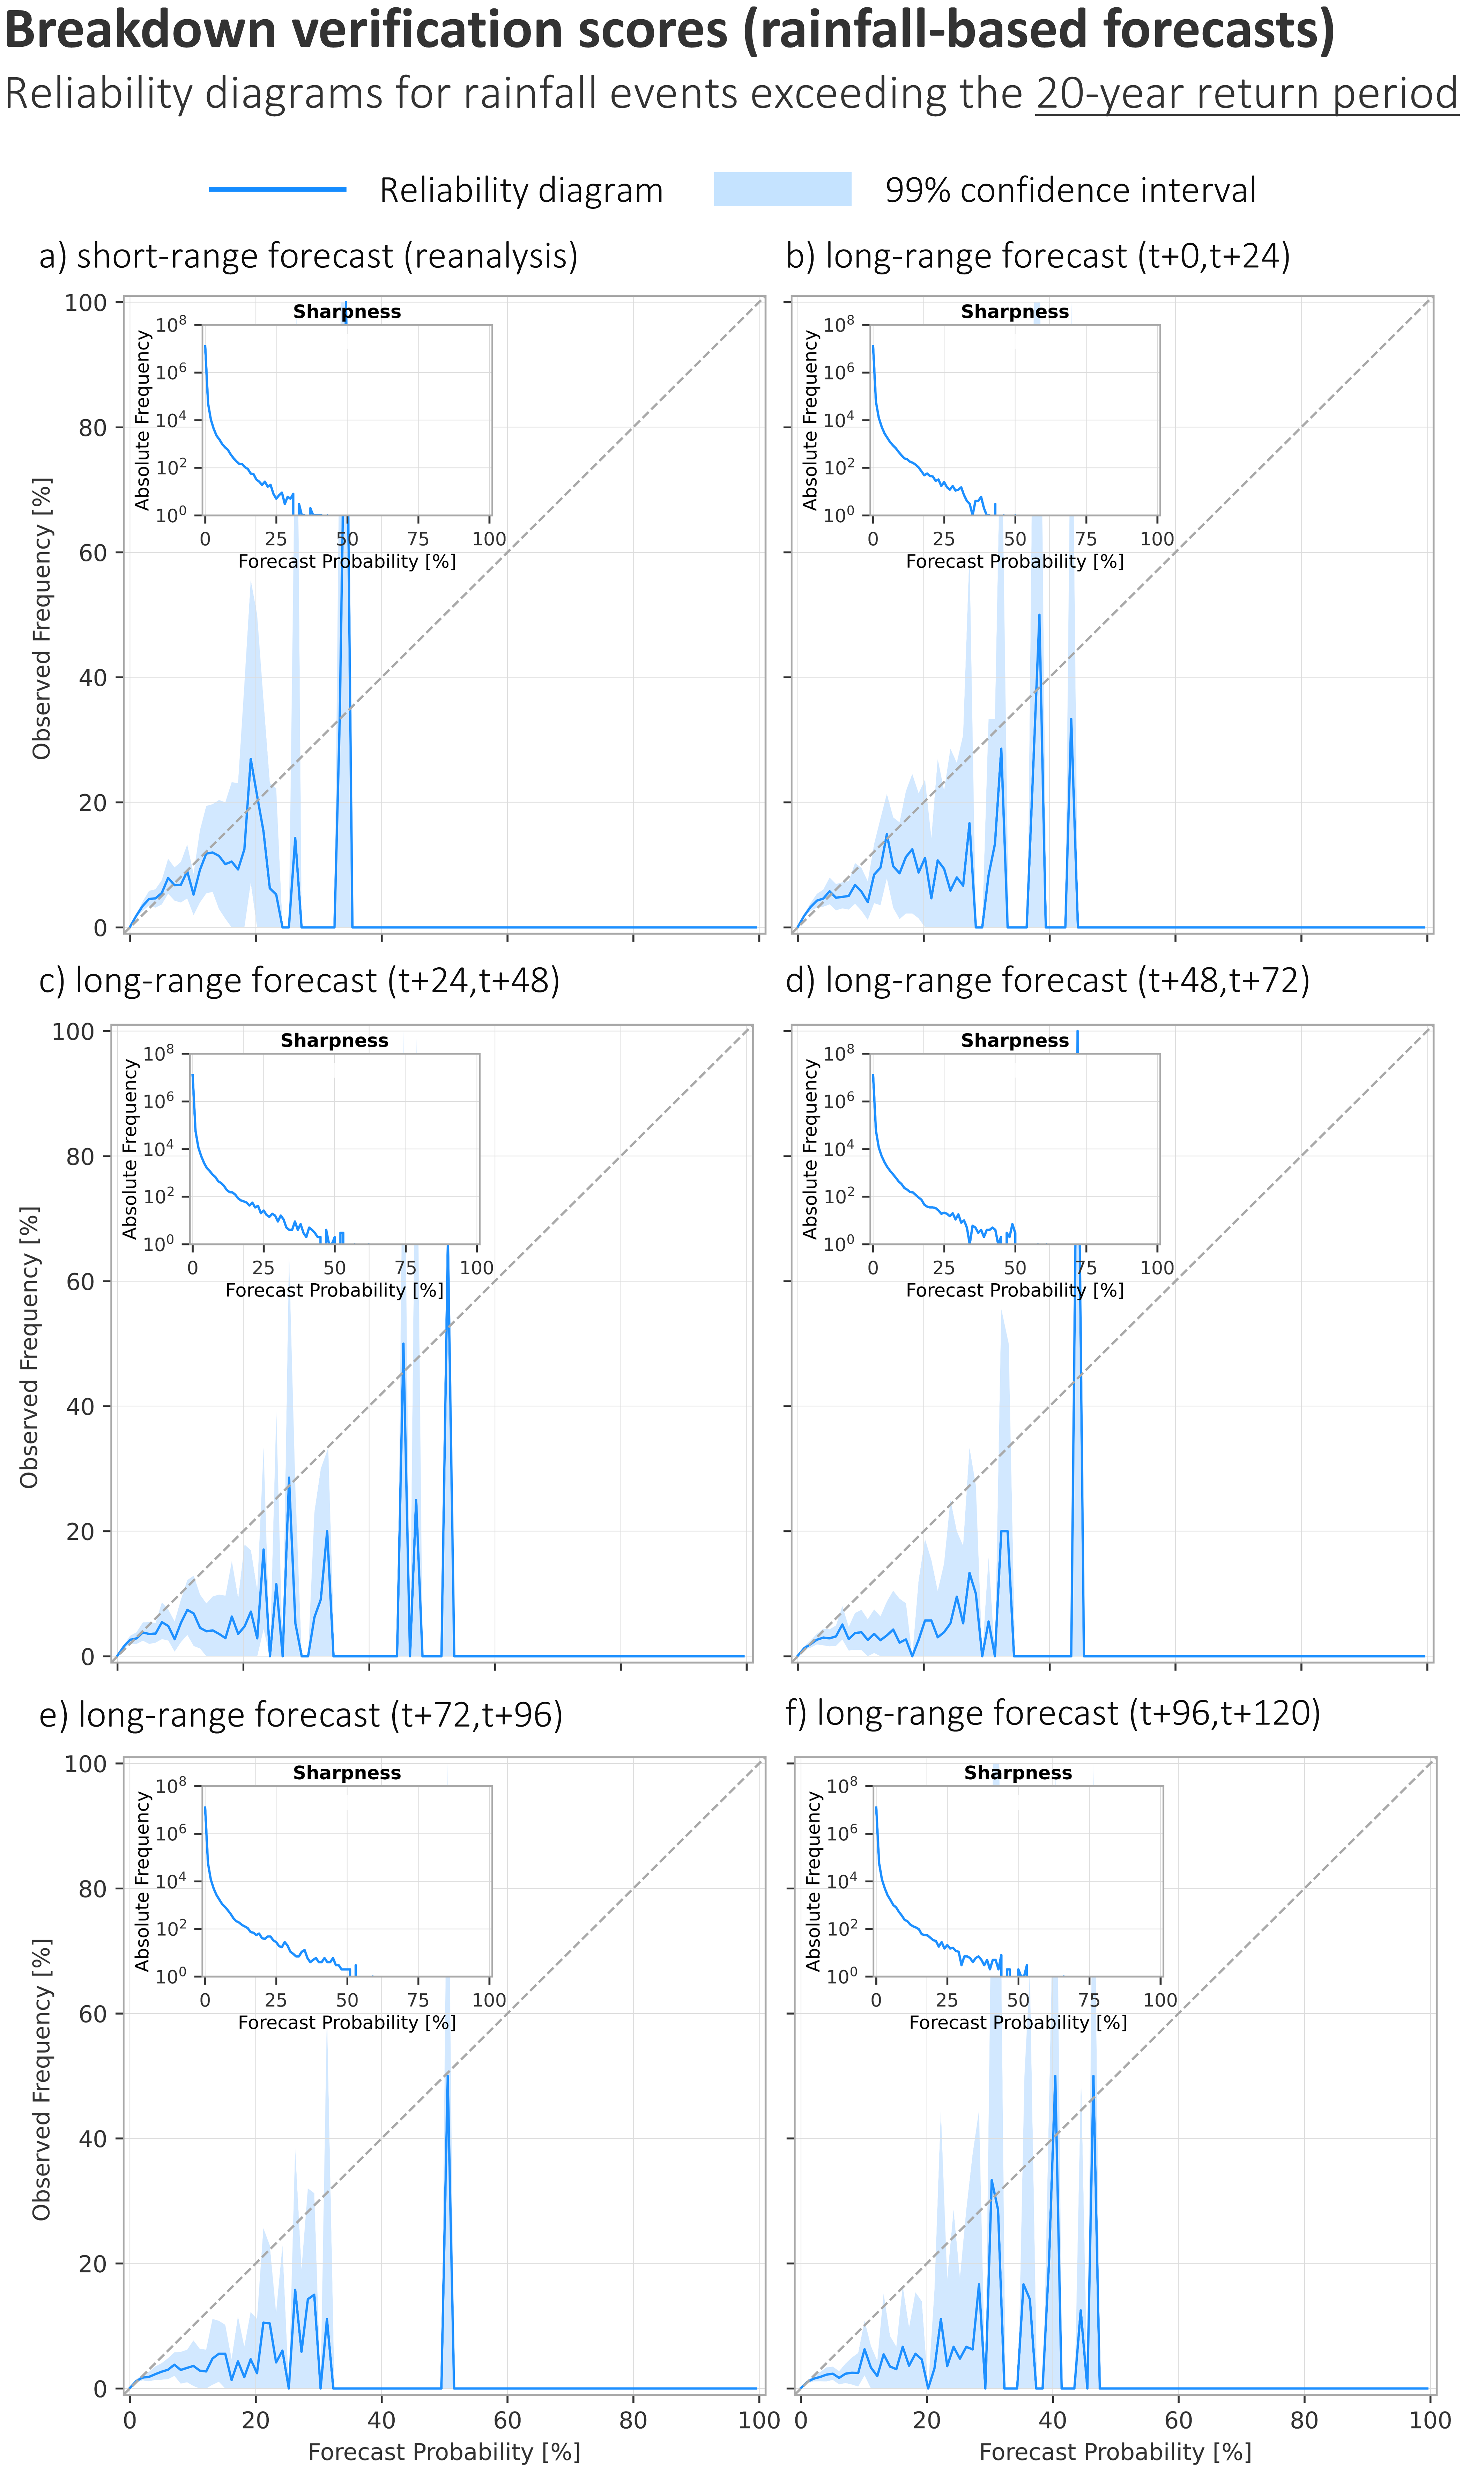
\includegraphics[width=\textwidth]{rainfall_based_ff_verif_breakdown_scores_rel_diag_20rp.png}
\caption{\textbf{Reliability diagrams for tp >= 5-year return period for the rainfall-based forecasts of areas at risk of flash floods built with ERA5-ecPoint.} Similar to Figure \ref{fig:rainfall_based_ff_verif_breakdown_scores_rel_diag_1rp}.}
\label{fig:rainfall_based_ff_verif_breakdown_scores_rel_diag_20rp}
\end{figure}

\begin{figure}[htbp]
\centering
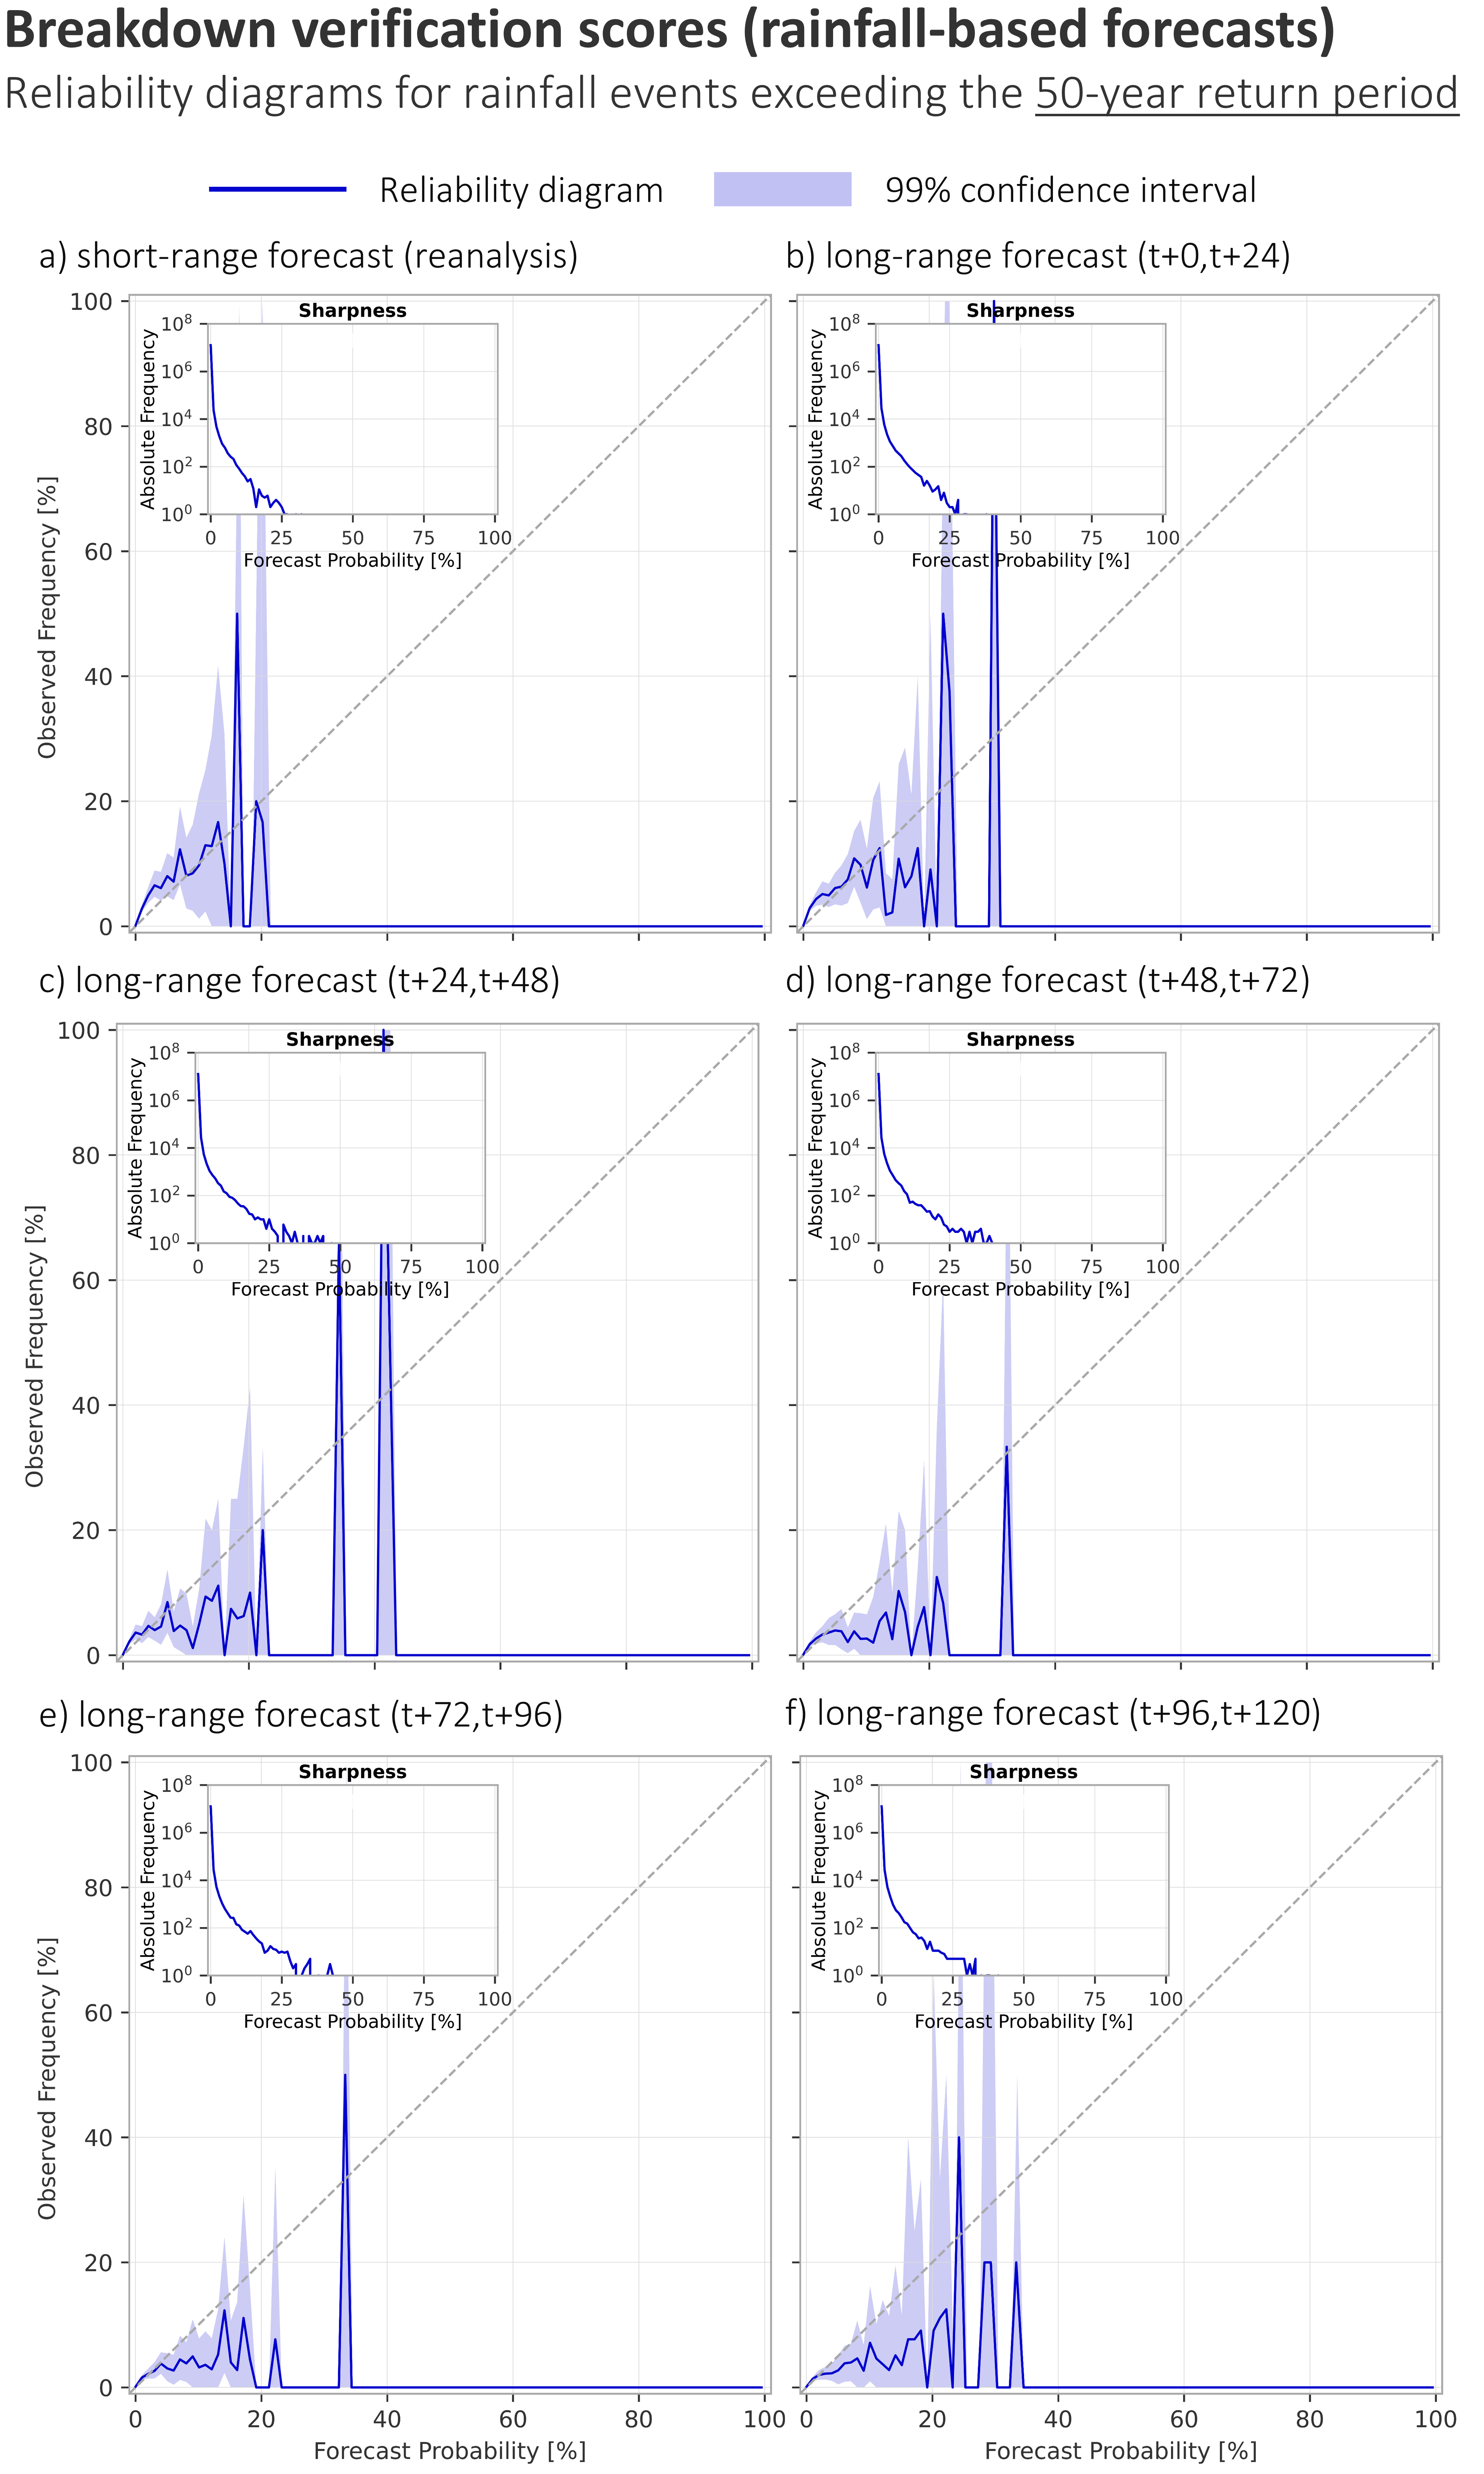
\includegraphics[width=\textwidth]{rainfall_based_ff_verif_breakdown_scores_rel_diag_50rp.png}
\caption{\textbf{Reliability diagrams for tp >= 5-year return period for the rainfall-based forecasts of areas at risk of flash floods built with ERA5-ecPoint.} Similar to Figure \ref{fig:rainfall_based_ff_verif_breakdown_scores_rel_diag_1rp}.}
\label{fig:rainfall_based_ff_verif_breakdown_scores_rel_diag_50rp}
\end{figure}

\begin{figure}[htbp]
\centering
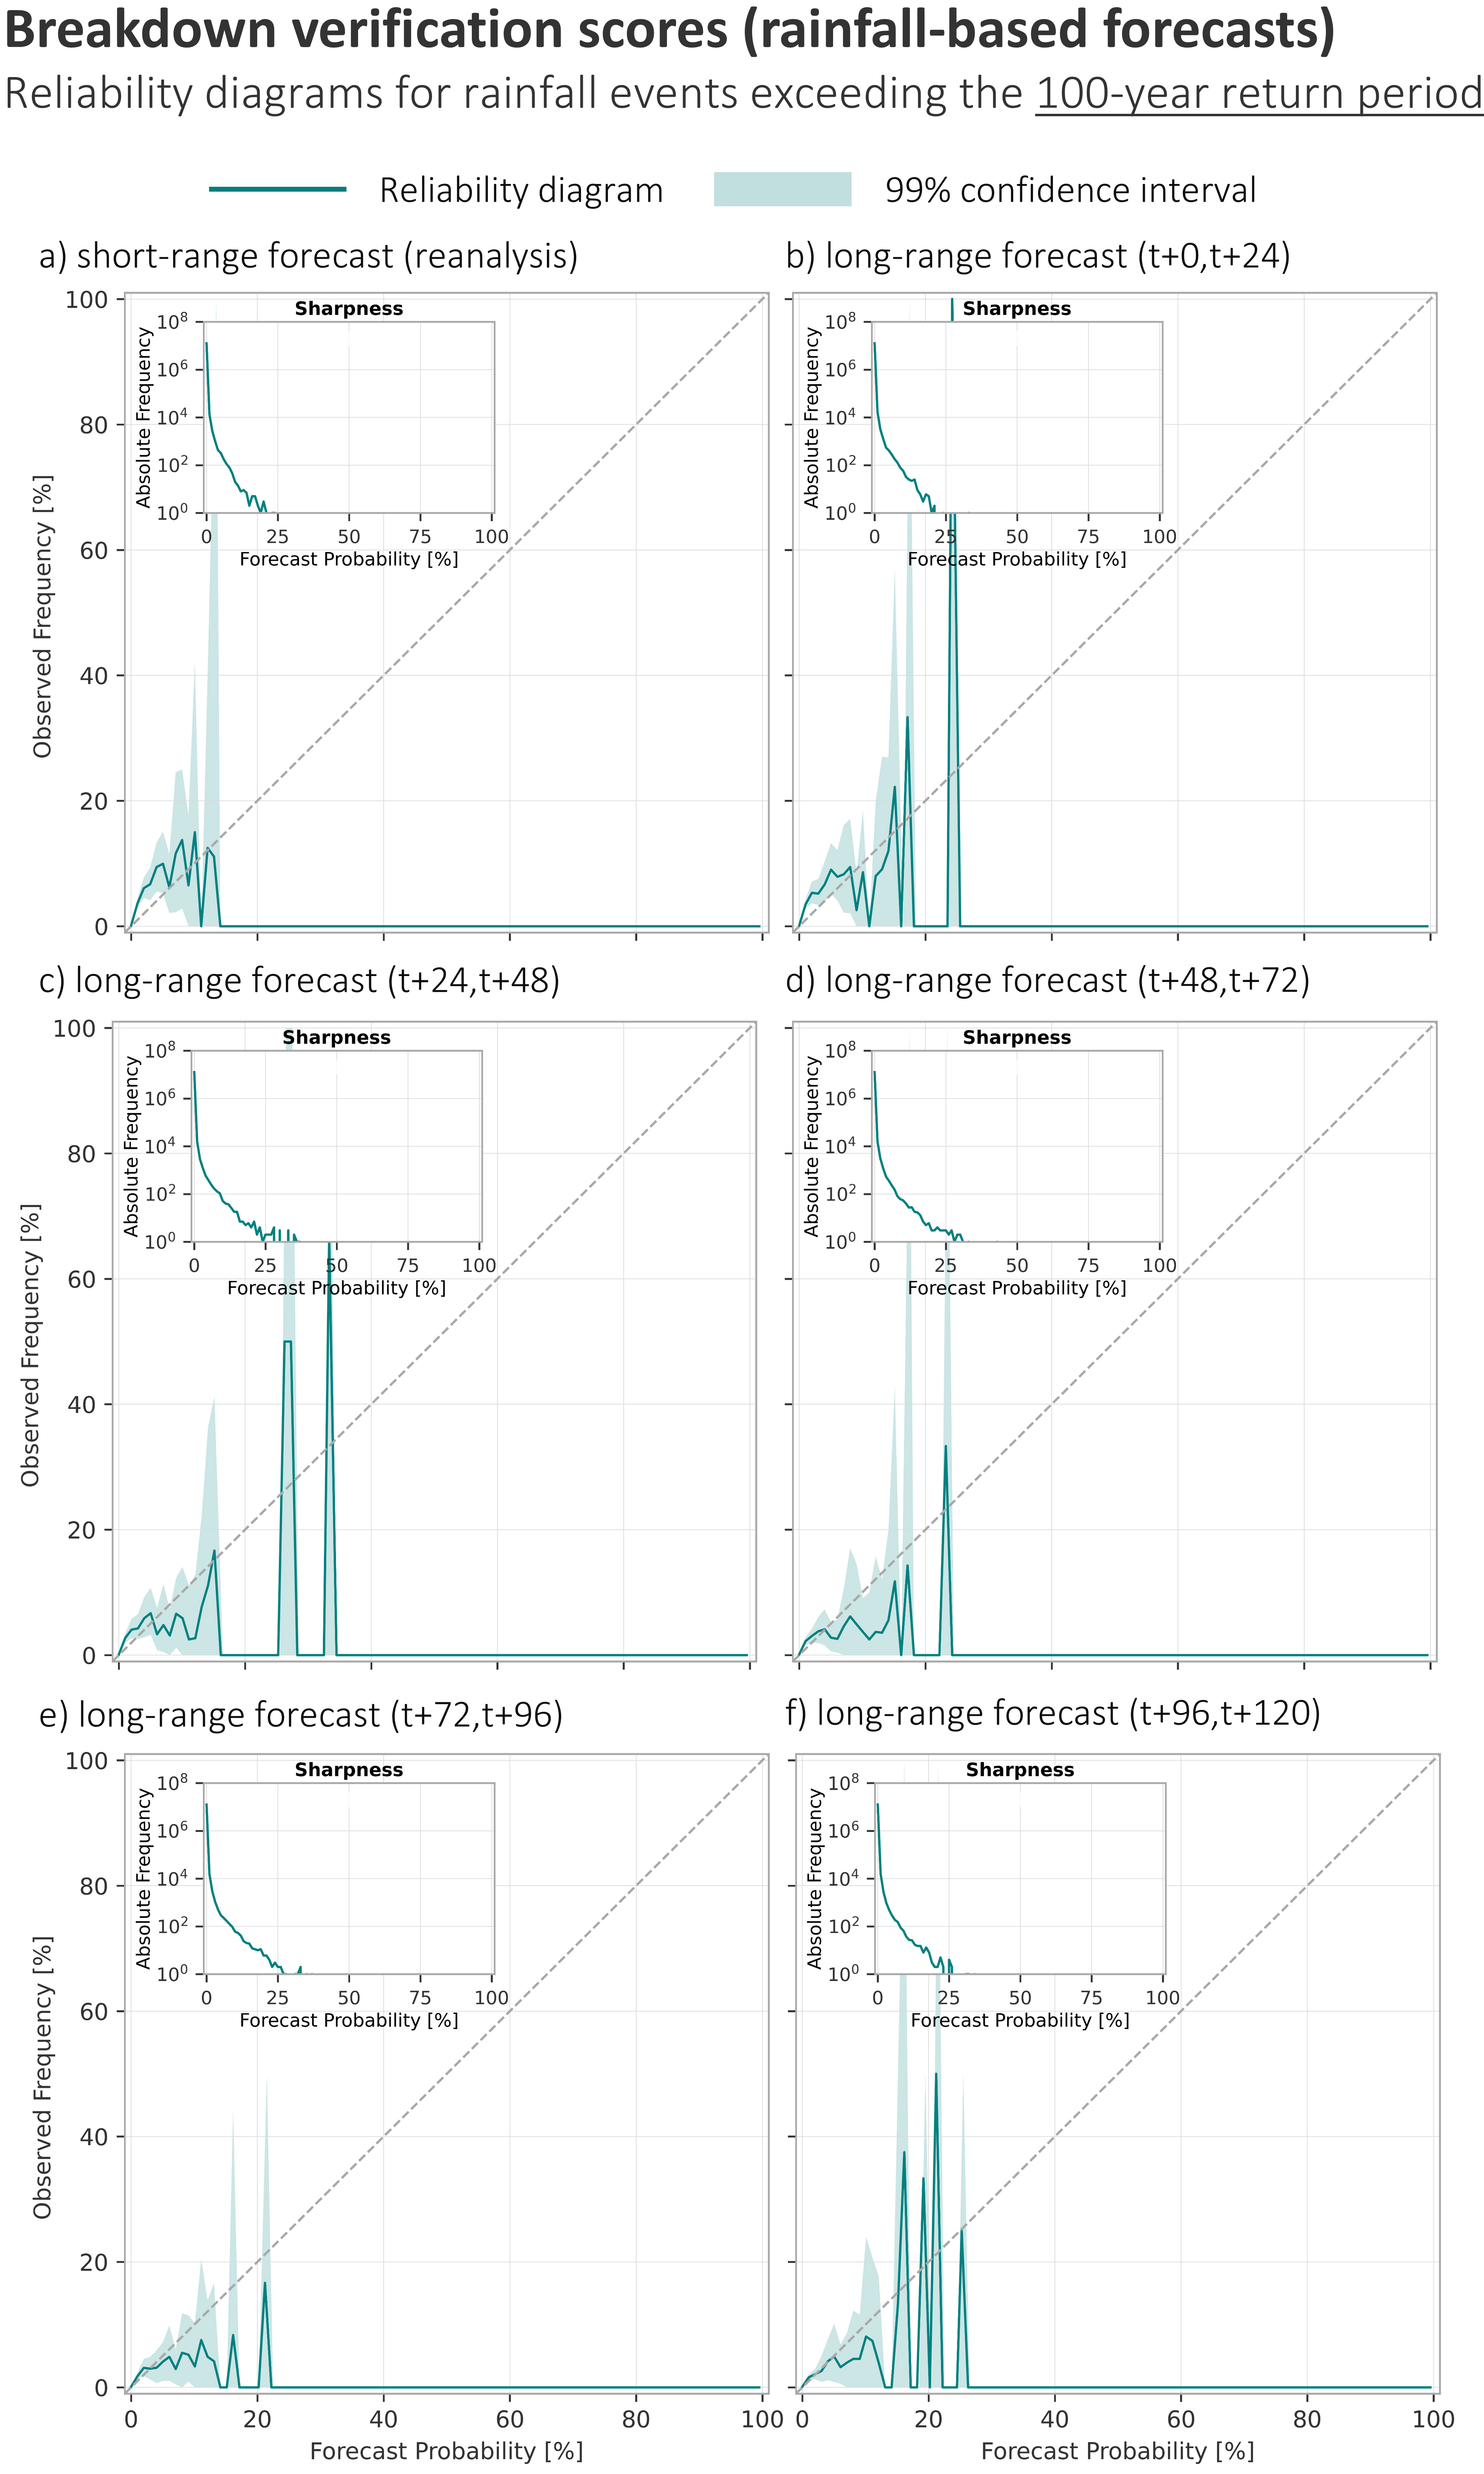
\includegraphics[width=\textwidth]{rainfall_based_ff_verif_breakdown_scores_rel_diag_100rp.png}
\caption{\textbf{Reliability diagrams for tp >= 5-year return period for the rainfall-based forecasts of areas at risk of flash floods built with ERA5-ecPoint.} Similar to Figure \ref{fig:rainfall_based_ff_verif_breakdown_scores_rel_diag_1rp}.}
\label{fig:rainfall_based_ff_verif_breakdown_scores_rel_diag_100rp}
\end{figure}

%%%%%%%%%
\section{Assessment of short-range data-driven hydro-meteorological predictions of areas at risk of flash floods}
\label{verif_data_driven_short_fc}

\subsection{Model training}

\subsection{Comparative performance analysis with the rainfall-based predictions}
\subsubsection{Discrimination ability}
\subsubsection{Reliability}

\subsection{Physical interpretation of the data-driven model behaviour}

\subsection{Extension of regional training to global application}


%%%%%%%%%
\section{Assessment of long-range data-driven hydro-meteorological predictions of areas at risk of flash floods}
\label{verif_data_driven_long_fc}

\subsection{Discrimination ability}

\subsection{Reliability}


%%%%%%%%%
\section{Catalogue of flash flood events}
\label{verif_case_study}       % Chapter 5
% %%%%%%%%%%%%%%%%%%%%%%%%%%%%%%%%%%%%%%%%%%%%%%%%%%%%%%%%%%%%%%%%%%%%
\chapter{Data-driven probability of flash flood: how feasible?}
\label{feasibility_PoFF}
\graphicspath{{chapter_06/figures}{chapter_06/tables}}
%%%%%%%%%%%%%%%%%%%%%%%%%%%%%%%%%%%%%%%%%%%%%%%%%%%%%%%%%%%%%%%%%%%%


For hydro-meteorological, data-driven predictions, the verifying thresholds emerge directly from the machine learning algorithms that generated the predictions themselves, applying an optimisation that establishes the probability values that maximise the F1-score when converting a probabilistic prediction into a yes- or non-event. This data-driven threshold selection represents a departure from traditional approaches based, for example, on assumptions about the severity of the triggering events (as done for the rainfall-based forecasts). It instead allows the data-driven models itself to identify optimal decision boundaries to convert the probabilistic forecasts into a yes- or a non-event. As such, the thresholds will be defined based on the frequency of the yes-events in the observational datasets, delivering smaller verifying thresholds for rarer events. 



\subsection{Which verification metrics provide a comprehensive assessment of forecast quality?}

The verification framework employs a suite of metrics designed to evaluate different aspects of forecast performance, recognising that no single metric can fully characterise prediction quality for rare events like flash floods (pink area in Figure \ref{fig:workflow_verif_framework}). The selection of metrics addresses two primary forecast attributes: reliability and discrimination ability.

Reliability assessment examines whether predicted probabilities accurately reflect observed frequencies. The frequency bias provides an aggregate measure of systematic over- or under-prediction, whilst reliability diagrams offer detailed insights into calibration across the full probability spectrum. These metrics prove particularly valuable for understanding how well forecast systems capture the climatological frequency of flash floods, a fundamental requirement for risk-based decision making.

Discrimination ability quantifies the forecast system's capacity to distinguish between flood and non-flood situations. The Area Under the Receiver Operating Characteristic curve (AROC) provides a threshold-independent summary measure, whilst the full ROC curve reveals performance trade-offs at different probability thresholds. For rare event prediction, discrimination ability often represents the primary challenge, as models must identify subtle signals preceding infrequent occurrences.

The choice of probabilistic metrics reflects the inherent uncertainty in flash flood prediction and the need for risk-based decision frameworks in operational contexts. Deterministic metrics prove less suitable given the rarity of events and the importance of capturing forecast uncertainty. Detailed mathematical formulations and computational procedures are provided in the relevant analysis chapters.




\subsection{What training strategy ensures robust assessment of model performance when working with an extremely imbalanced dataset?}

The validation framework employs nested cross-validation with hyperparameter optimisation to provide unbiased performance estimates whilst maximising model performance. This approach addresses the risk of overfitting inherent in machine learning applications to imbalanced datasets.

The outer cross-validation loop uses stratified k-fold splitting to ensure representative class distributions in all data partitions. Within each outer fold, an inner optimisation loop identifies optimal hyperparameters using Bayesian optimisation via the Optuna framework. This nested structure prevents information leakage between hyperparameter selection and performance evaluation, providing realistic estimates of operational performance.
The choice of AROC as the optimisation metric during hyperparameter tuning reflects its suitability for imbalanced classification and alignment with the verification framework. Alternative metrics such as F1-score prove less suitable due to their dependence on classification thresholds and potential instability with extreme class imbalance.

Repeated evaluation across multiple cross-validation folds quantifies performance variability and identifies potential instabilities in model training. This comprehensive validation approach ensures that reported performance metrics reflect genuine predictive capability rather than fortunate data splits or overfitting to specific training samples. Implementation details and computational considerations are discussed in Chapter \ref{feasibility_PoFF}.



\subsection{How should flash flood observations be processed for grid-based verification?}

The transformation of point-based impact reports into gridded observational fields requires careful consideration of spatial and temporal aggregation methods. This study implements a systematic approach aligned with established severe weather verification methodologies \citep{Tsonevsky_2018, Pillosu_2024}.

Each flash flood report undergoes temporal aggregation to match the 24-hour accumulation periods of the forecast products, beginning at 00 UTC. This alignment ensures consistent comparison between observations and predictions whilst acknowledging that flash floods may occur at any time within the accumulation window. The choice of 24-hour periods balances the need for sufficient temporal resolution with the practical constraints of forecast product availability and the typical duration of flash flood events.

Spatial assignment of reports to the ERA5 grid (approximately 31 km resolution) employs a nearest-neighbour approach for point reports and polygon inclusion for events with spatial extent. Given the relatively coarse resolution of ERA5 grid boxes compared to typical flash flood scales, additional spatial expansion techniques commonly used in convective-scale verification prove unnecessary. The resulting gridded fields preserve information about event frequency within each grid box, enabling more nuanced verification than binary occurrence fields.
This processing approach addresses the fundamental challenge of scale mismatch between localised flash flood events and gridded forecast products. The methodology provides a reproducible framework applicable to other grid resolutions and accumulation periods, with detailed implementation provided in chapter \ref{flash_flood_focused_verification_framework}.

       % Chapter 6
% %%%%%%%%%%%%%%%%%%%%%%%%%%%%%%%%%%%%%%%%%%%%%%%%%%%%%%%%%%%%%%%%%%%%\chapter{Data-driven probability of flood: what predictability?}
\label{predictability_PoFF}
\graphicspath{{chapter_07/figures}{chapter_07/tables}}
%%%%%%%%%%%%%%%%%%%%%%%%%%%%%%%%%%%%%%%%%%%%%%%%%%%%%%%%%%%%%%%%%%%%       % Chapter 7
% %%%%%%%%%%%%%%%%%%%%%%%%%%%%%%%%%%%%%%%%%%%%%%%%%%%%%%
\chapter{General discussions}
\label{general_discussions}
\graphicspath{{chapter_08/figures}{chapter_08/tables}}
%%%%%%%%%%%%%%%%%%%%%%%%%%%%%%%%%%%%%%%%%%%%%%%%%%%%%%



\section{Contributions to knowledge and practice in flash flood prediction}


% Material to re-read
The unprecedented convergence of three key scientific advancements — the demonstrated effectiveness of index-based flash flood forecasting systems, improvements in global NWP rainfall predictions, and the rise of data-driven approaches — has created a unique opportunity to address the critical challenge of developing medium-range flash flood forecasts with global coverage. This thesis seizes this opportunity by systematically investigating the research gaps, challenges, and objectives identified in the previous sections. This research significantly contributes to the scientific understanding and practical implementation of flash flood prediction systems by developing a flash-flood-focused verification framework, assessing data-driven models' capability to identify areas at risk, and evaluating the predictability of medium-range forecasts. These contributions come at a critical juncture, as the increasing frequency and severity of flash floods worldwide have created an urgent need for improved prediction and early warning capabilities. The UN's "Early Warnings for All" initiative has further highlighted the pressing need to extend these life-saving capabilities to historically underserved regions. This thesis directly supports the global effort to protect vulnerable communities through enhanced flash flood prediction by addressing fundamental research gaps and developing innovative methodologies. The timeliness and relevance of this work cannot be overstated, as it provides essential tools and insights for mitigating the devastating impacts of flash floods in a changing climate.

This \marginpara{Contribution no. 1: scientific contribution to flash flood prediction} thesis advances the scientific understanding of flash flood prediction in several key ways. First, it introduces a novel verification framework that directly evaluates global NWP rainfall forecasts against flash flood impacts, moving beyond traditional rainfall-to-rainfall verification approaches (RG1). This methodological advancement is significant, as it directly assesses the usefulness of global NWP rainfall forecast for flash flood prediction, especially at medium-range timescales. By focusing on the relationship between forecasted rainfall and actual flash flood occurrences, this framework enables a more targeted evaluation of the global NWP rainfall forecasts' performance. The insights gained from this approach are crucial for guiding improvements in NWP models and post-processing techniques, ensuring that advancements in rainfall prediction translate into tangible benefits for flash flood early warning. Second, the research demonstrates the feasibility of using data-driven approaches for flash flood prediction at a global scale (RG2). This is a major advancement, as data-driven methods have the potential to leverage the increasing availability of global datasets and computational resources to improve prediction accuracy and extend coverage to data-sparse regions. While significant progress has been made in the data-driven modelling of floods in larger catchments, it is important to note that few approaches have specifically focused on the unique characteristics and challenges associated with flash floods. Moreover, to the best of our knowledge, no existing studies have comprehensively investigated the optimal architecture or data-driven approach for flash flood forecasting. This thesis addresses this critical gap by developing and evaluating innovative methodologies tailored to the distinct nature of flash flood events. By considering the specific challenges posed by flash floods, such as their rapid onset, short duration, and localised impacts, this research contributes novel insights into the design and implementation of effective data-driven models for flash flood prediction. The thesis explores various architectures and training strategies, systematically assessing their performance and suitability for capturing the complex dynamics of flash flood processes. This rigorous evaluation identifies the most promising approaches for operational implementation, providing a solid foundation for future research and development in this field. Third, through systematic evaluation of medium-range forecast predictability (RG3), this work establishes new frontiers in understanding the practical limits and opportunities of extending flash flood predictions beyond traditional short-term forecasts. Medium-range forecasting has long been challenging for flash flood prediction due to the inherent uncertainties associated with longer lead times. By rigorously assessing the predictability of these forecasts, this thesis provides valuable insights into the reliability and uncertainty of medium-range predictions. This knowledge is essential for informing the operational implementation of medium-range forecasting systems, helping decision-makers understand the trade-offs between lead time and accuracy. Additionally, identifying predictability limits helps to guide future research efforts to push the boundaries of flash flood prediction.

The \marginpara{Contribution no. 2: practical implications for global flash flood early warning} demonstrated feasibility of data-driven approaches for global flash flood prediction offers a practical pathway for developing scalable flash flood early warning systems providing medium-range forecasts with global coverage. The findings presented in this thesis have far-reaching implications in regions where traditional approaches may be constrained by data availability or computational limitations, as data-driven methods can leverage globally available datasets and cloud computing to provide cost-effective prediction capabilities. By demonstrating how these methods can be applied to flash flood prediction globally, this thesis aligns directly with the UN's "Early Warnings for All" initiative, potentially enabling the extension of life-saving early warnings to historically underserved communities. The assessment of medium-range predictability conducted in this thesis provides a foundation for future research on the operational usability of data-driven medium-range flash flood forecasts. By evaluating the performance of these medium-range predictions, this work offers valuable insights into the potential benefits and limitations of incorporating longer-lead forecasts into early warning systems. While the thesis does not directly engage stakeholders or decision-makers to determine how they would utilise these medium-range forecasts, the findings presented here can inform future studies on the forecasts' practical application and communication. The insights gained from the predictability assessment can guide the development of early warning protocols and communication strategies that effectively convey the increased uncertainty associated with longer-lead predictions. By providing a realistic understanding of the capabilities and limitations of medium-range forecasts, this thesis lays the groundwork for future research on how to optimally integrate these forecasts into operational decision-making processes. This may involve investigating how to present forecast information that clearly communicates the associated uncertainties and exploring how decision-makers can effectively utilise medium-range predictions combined with other risk assessment tools and local knowledge. Furthermore, the findings of this thesis can inform future stakeholder engagement efforts, helping to ensure that the development and implementation of medium-range flash flood forecasting systems align with the needs and priorities of end-users. By providing a robust scientific foundation for understanding the predictability of medium-range forecasts, this work enables future targeted and effective communication with stakeholders about extended-range predictions' potential value and limitations. This can facilitate the co-development of early warning systems tailored to different communities' specific needs and contexts, ultimately enhancing the impact and effectiveness of flash flood risk reduction efforts.

%%%%%%%%%%%%%%%%%%%%%%%%%%%%%%%%%%%%%%%%%%%%%%%%%%%
\section{Policy and Governance in Flash Flood Management}
\subsection{International Coordination and Collaboration}
\subsubsection{Cross-Border Data Sharing}
Cross-border data sharing is a fundamental aspect of international coordination in flash flood management, enabling the integration of diverse datasets to enhance forecasting accuracy and preparedness. The exchange of flood-related information across national boundaries facilitates the development of comprehensive systems that can address the transnational nature of flash floods, which often impact multiple regions simultaneously due to shared hydrological and meteorological conditions. Such collaboration is particularly critical in areas where rivers and drainage basins traverse multiple countries, necessitating unified approaches to data collection, analysis, and dissemination. The INSPIRE platform exemplifies efforts to standardize and share flood maps across European nations, providing a centralized repository for exposure layers required in forecasting models \citep{Ritter2021a}\citep{Ritter2021b}. This initiative underscores the importance of harmonized data formats and accessibility in fostering large-scale forecasting solutions. By enabling countries to contribute their national flood maps, INSPIRE supports the preprocessing of exposure layers essential for systems like ReAFFINE, which aim to expand their operational scope over broader spatial domains \citep{Ritter2021a}\citep{Ritter2021b}. These standardized practices not only streamline data integration but also reduce redundancies and inconsistencies that could hinder model performance. Effective cross-border data sharing also requires addressing challenges related to data quality and observational limitations. For instance, radar-based quantitative precipitation estimates (QPE) have been identified as preferable for ensuring consistent rainfall thresholds in flash flood prediction models. However, disparities in technological capabilities among nations can lead to uneven data quality, complicating efforts to establish reliable early warning systems. Additionally, uncertainties in rainfall inputs and limited streamflow observations further exacerbate these challenges \citep{Msigwa2024}. Collaborative investments in advanced monitoring technologies and training programs can mitigate such disparities, ensuring that all participating countries contribute high-quality datasets. Legal frameworks play a crucial role in facilitating cross-border data sharing by establishing protocols for cooperation and enforcement. The authors of \citep{Saad2024} highlight the necessity of clear communication mechanisms among stakeholders to address common challenges in river and drainage management. Extending this principle to international contexts involves creating agreements that define responsibilities for data provision, usage rights, and confidentiality measures. Such frameworks not only promote trust among nations but also ensure compliance with ethical standards governing the use of shared information. The integration of historical flash flood inventories with geo-environmental conditioning factors offers another avenue for enhancing cross-border forecasting capabilities. By analyzing past events under similar environmental conditions, researchers can identify patterns that inform predictive models applicable across regions. This approach assumes that future flash floods will be governed by analogous factors as those observed historically \citep{Ngo2018}, making it imperative for countries to share detailed inventories and environmental datasets. Despite these advancements, policy fragmentation remains a significant barrier to effective cross-border collaboration. Coordination between federal, state, and local governments within individual countries must align with international efforts to ensure cohesive strategies for flood risk management. Regular updates to policy frameworks are necessary to reflect evolving climate patterns and urban dynamics that influence flash flood occurrences \citep{Saad2024}. Without such alignment, discrepancies between national policies can undermine the effectiveness of shared systems. The implementation of automated systems like ALERT in the United States and HYDRATE in Europe demonstrates practical applications of large-scale data recording for heavy rainfall events \citep{Khan2020}. These systems rely on real-time observations transmitted across networks to provide timely warnings. Expanding similar technologies globally requires robust infrastructure capable of handling high volumes of data while maintaining interoperability across different platforms. Collaboration among local authorities within transboundary regions further emphasizes the importance of cross-border data sharing. Effective river management often depends on coordinated efforts among municipalities traversed by shared waterways. Extending this principle internationally involves fostering partnerships among neighboring countries to manage rivers collectively while addressing pollution, erosion, and other environmental concerns impacting residents' well-being \citep{Saad2024}. Standardizing methodologies for assessing vulnerability through indices like FI-D-F curves derived from rainfall intensity-duration-frequency relations can also benefit from cross-border cooperation \citep{Kim2011}. Sharing these analytical tools enables countries to adopt consistent metrics for evaluating flash flood risks under varying climatic conditions. In summary, cross-border data sharing is indispensable for advancing global flash flood forecasting systems. It requires harmonized platforms like INSPIRE \citep{Ritter2021a}\citep{Ritter2021b}, investments in advanced monitoring technologies \citep{Msigwa2024}, legal frameworks promoting cooperation \citep{Saad2024}, integration of historical inventories with predictive models \citep{Ngo2018}, alignment of policies across governance levels \citep{Saad2024}, implementation of automated observation systems \citep{Khan2020}, collaborative river management strategies \citep{Saad2024}, and standardized vulnerability assessment methodologies \citep{Kim2011}.
\subsubsection{Global Standards for Forecasting Systems}
Global standards for forecasting systems are essential to ensure consistency, reliability, and effectiveness in mitigating flash flood risks across diverse geographical regions. The development of such standards requires a comprehensive understanding of flash flood dynamics, including meteorological and hydrological factors that influence their occurrence and severity. Flash floods are highly localized phenomena, often triggered by extreme rainfall events that interact with specific basin characteristics, impervious surfaces, and urbanization patterns \citep{Saad2024}\citep{Yussouf2020}. These factors necessitate adaptable forecasting systems capable of addressing spatial variability and temporal unpredictability. International coordination plays a significant role in establishing global standards for flash flood forecasting systems. Collaborative efforts among nations enable the sharing of data, methodologies, and technological advancements, which are critical for improving forecasting accuracy. For instance, China's collaboration with multiple countries highlights the importance of international partnerships in producing impactful research and advancing forecasting capabilities \citep{Hinge2024}. Such collaborations foster the exchange of expertise and resources, leading to the development of robust models tailored to regional needs. The integration of early warning systems into global forecasting frameworks is another crucial aspect. Effective early warning systems rely on accurate hazard monitoring, timely dissemination of warnings, and clear communication with stakeholders. These systems must account for user-specific requirements and operational constraints while addressing uncertainties inherent in forecasting processes. The United Nations International Strategy on Disaster Reduction emphasizes the need for coordinated efforts across monitoring services, communication channels, and decision-making processes to enhance disaster preparedness \citep{Jubach2016}. Existing flash flood forecasting systems vary significantly in their spatial domain coverage, output uncertainty management, and model implementation strategies. For example, ensemble flood forecasting approaches provide probabilistic predictions that account for uncertainties in rainfall intensity and antecedent soil moisture conditions \citep{Luong2021}\citep{Naulin2013}. These methods utilize thresholds derived from hydrological analyses to issue warnings when critical discharge levels are exceeded. However, challenges remain in accurately predicting localized extreme rainfall events due to limitations in data quality and computational resources \citep{Hinge2024}. The FLASH project exemplifies advancements in providing forecasters with decision-support tools tailored to flash flood warnings in the United States \citep{Flamig2020}. Such initiatives underscore the importance of developing standardized tools that can be adapted globally while maintaining regional specificity. Furthermore, hydrological nowcasting chains have been proposed as effective mechanisms for real-time flood risk assessment by integrating rainfall forecasts with basin-scale hydrological models \citep{Silvestro2017}. These approaches highlight the need for harmonized methodologies that balance precision with scalability. Despite progress in forecasting technologies, significant challenges persist in implementing global standards. Variations in data availability across regions complicate model calibration and validation processes \citep{Hinge2024}. Additionally, discrepancies in construction standards, legal enforcement mechanisms, and developer practices exacerbate vulnerabilities to flash floods \citep{Saad2024}. Addressing these issues requires coordinated policy frameworks that align national regulations with international best practices. Efforts to establish global standards must also consider socio-economic dimensions. Quantitative assessments of the costs and benefits associated with early warning systems can inform policy decisions aimed at optimizing resource allocation \citep{Jubach2016}. Moreover, understanding user-specific needs ensures that warnings are actionable and effective across diverse populations. The EWIN system implemented in Mexico demonstrates how localized solutions can contribute to broader standardization efforts by integrating weather data into scalable models designed for wider applications \citep{Msigwa2024}. In summary, global standards for flash flood forecasting systems necessitate international collaboration to harmonize methodologies while accommodating regional variability. Advances in ensemble modeling techniques, early warning system components, and real-time decision-support tools provide a foundation for developing consistent frameworks capable of reducing flash flood impacts worldwide \citep{Flamig2020}\citep{Jubach2016}\citep{Silvestro2017}\citep{Luong2021}.
\subsubsection{Collaboration in Research and Development}
Collaboration in research and development plays a crucial role in advancing the understanding and management of flash floods, particularly through international coordination efforts. Effective collaboration fosters the exchange of knowledge, resources, and expertise among researchers, institutions, and nations, enabling the development of innovative solutions to address the multifaceted challenges posed by flash floods. The authors of \citep{Hinge2024} highlight that international partnerships significantly contribute to producing highly cited articles, demonstrating the positive correlation between collaborative efforts and impactful scientific outcomes. Such partnerships not only enhance the quality of research but also facilitate the integration of diverse perspectives and methodologies. The importance of collaboration extends beyond academic contributions; it is essential for addressing practical challenges in flash flood forecasting systems. According to, local authorities must share information and work together to manage rivers and drainage systems effectively. This cooperation is critical for mitigating flooding risks, pollution, erosion, and other environmental issues that affect communities' well-being. The complexities arising from rivers traversing multiple administrative regions underscore the necessity for coordinated management strategies that transcend jurisdictional boundaries. Furthermore, collaboration can foster a sense of ownership among stakeholders while promoting public awareness and participation in conservation efforts. By establishing clear mechanisms for communication, coordination, cooperation, and enforcement, local authorities can address common challenges more effectively. This approach not only strengthens governance structures but also ensures that policies are implemented consistently across different regions. Despite these benefits, challenges remain in achieving seamless collaboration. Policy fragmentation often hinders integration efforts at various levels of governance. For instance, while national policies may provide strategic direction for sustainable urban growth, their effectiveness depends on alignment with local-level implementation frameworks such as drainage guidelines and stormwater management standards \citep{Saad2024}. Improved coordination between federal, state, and local governments is necessary to align development goals with flood risk considerations while adapting policies to changing climate patterns. International collaboration also plays a vital role in enhancing early warning systems for flash floods. Researchers emphasize the need for these systems to account for local time scales, geography, climate variables, data availability, and predictive uncertainty \citep{Henao2022}\citep{Henao2022a}. Collaborative efforts can help design tailored methodologies that maximize the accuracy and reliability of warning systems by leveraging shared expertise across regions with varying hydrological characteristics. Moreover, advancements in soft computing techniques for flood susceptibility mapping have been limited by insufficient exploration of collaborative dynamics between authors from countries with fewer publications \citep{Hinge2024}. Addressing this gap through targeted international partnerships could lead to more comprehensive analyses that consider factors such as topography, climatic conditions, basin characteristics, and implementation scale. The integration of disaster management policies further illustrates the significance of collaboration. Activities such as reviewing existing plans and analyzing linkages between providers and users of severe weather warnings require coordinated efforts across national-to-community levels \citep{Jubach2016}. These activities ensure that emergency protocols are robustly designed to respond effectively to flash flood events. Finally, ongoing research initiatives demonstrate how collaboration can improve forecasting models despite inherent uncertainties. For example, simple frameworks based on accumulated upstream precipitation have been justified due to uncertainties in ensemble weather predictions \citep{Alfieri2015}. Collaborative projects like IMPRINTS have shown promising results in refining these models through shared data assimilation methods \citep{Naulin2013}. In summary, collaboration in research and development is indispensable for advancing flash flood management strategies. It enables the pooling of resources across disciplines and regions while addressing both theoretical foundations and practical applications. By fostering international coordination among researchers and policymakers alike, collaborative efforts pave the way for innovative solutions that mitigate flash flood impacts effectively.

I'll reformat this section on national-level policies and frameworks, changing the citation style from \parencite{} to \citep{} and updating to the author-year format:
\subsection{National-Level Policies and Frameworks}
\subsubsection{Disaster Risk Reduction Strategies}
Disaster risk reduction strategies at the national level are essential for mitigating the impacts of flash floods, which are among the most destructive hydrological disasters. These strategies often involve a combination of policy frameworks, infrastructure development, and community engagement to enhance resilience and preparedness. The Sendai Framework for Disaster Risk Reduction (SFDRR) provides a comprehensive global guideline that nations can adapt to their specific contexts. It emphasizes reducing disaster risks through early action, improved forecasting systems, and proactive measures to safeguard lives, livelihoods, and critical assets. Early warning systems are a cornerstone of this framework, enabling timely dissemination of information to communities at risk. By fostering collaboration between meteorological agencies and local governments, these systems can significantly reduce casualties and economic losses associated with flash floods \citep{Jubach2016}\citep{Munoz2018}. In Malaysia, addressing flash flood risks has been prioritized through sustainable land management practices and disaster risk reduction policies. These measures include revisiting urban planning frameworks to account for flood-prone areas and implementing land use planning that minimizes exposure to hazards. Such approaches not only mitigate immediate risks but also contribute to long-term resilience by integrating environmental sustainability into development projects \citep{Saad2024}. The repair and maintenance of civil infrastructure play a crucial role in reducing vulnerability to flooding. In the United States, flooding is recognized as the second deadliest weather-related hazard after heat waves. Proactive floodplain management efforts under programs like the National Flood Insurance Program (NFIP) have demonstrated effectiveness in decreasing flood-related fatalities by promoting better infrastructure design and community preparedness \citep{Abegaz2024}. These initiatives highlight the importance of integrating engineering solutions with policy measures to address both structural and non-structural aspects of disaster risk reduction. Flash flood forecasting systems are another critical component of national-level strategies. Emerging machine learning techniques such as random forest algorithms have shown promise in improving short-term runoff predictions. However, challenges remain in accurately assessing localized extreme rainfall events due to model complexities and data limitations. Expanding rain gauge networks and incorporating remote sensing technologies can enhance forecasting accuracy while addressing spatial uncertainties \citep{Munoz2018}. This underscores the need for continuous investment in technological advancements to refine predictive models. The coupling of flash floods with sediment movement in mountainous regions further complicates disaster management efforts. Sediment transport during flash floods amplifies their destructive potential, necessitating targeted interventions such as sediment control structures and watershed management plans \citep{Yang2022}. These measures require coordination across multiple sectors, including hydrology, geology, and urban planning. Policy implications derived from international directives like the European Union Flood Directive also provide valuable insights into effective flood risk management. For instance, Spain's implementation of flood risk management plans has demonstrated how structured water planning cycles can align national policies with regional needs while ensuring compliance with broader legislative frameworks \citep{Bodoque2019}. Such examples illustrate how countries can leverage international guidelines to develop tailored strategies that address their unique vulnerabilities. Historical events have shaped national approaches to disaster risk reduction by highlighting gaps in existing systems. For example, significant floods like California's Central Valley Flood in 1862 have influenced U.S. flood management policies over time by underscoring the importance of robust infrastructure and adaptive planning \citep{Abegaz2024}. Learning from past disasters enables policymakers to refine strategies and build more resilient communities. Civil unrest stemming from inadequate transparency in infrastructure projects further emphasizes the need for accountability among developers and governing bodies. Ensuring public trust through participatory decision-making processes can enhance societal acceptance of disaster mitigation measures while fostering cooperation between stakeholders. This approach aligns with broader goals of sustainable development by balancing economic growth with environmental protection. By synthesizing these elements - policy frameworks like SFDRR, technological innovations in forecasting systems, proactive infrastructure maintenance, sediment control measures, historical lessons, and community engagement - nations can develop comprehensive strategies that effectively reduce flash flood risks while promoting resilience at all levels \citep{Saad2024}\citep{Jubach2016}\citep{Munoz2018}.
\subsubsection{Integration of Forecasting Systems into Policy}
The integration of forecasting systems into policy frameworks is essential for enhancing national-level strategies aimed at mitigating the impacts of flash floods. Forecasting systems provide critical data that can inform decision-making processes, enabling policymakers to implement measures that reduce vulnerability and improve preparedness. The operationalization of these systems within policy structures requires a multidisciplinary approach, combining meteorological, hydrological, and infrastructural insights to ensure their effectiveness. Early warning systems play a significant role in this integration by facilitating timely dissemination of information to relevant stakeholders. According to, the description and operation of early warning systems are key elements in national policies, emphasizing the need for integrating local data with broader forecasting models such as SWFDP and SARFFG. This integration ensures that forecasts are not only accurate but also contextually relevant, addressing localized risks effectively. Furthermore, responsibilities are distributed across various operational components, including forecast centers and disaster management agencies at national, provincial, and local levels \citep{Jubach2016}. Such distribution underscores the importance of clear communication channels and coordinated efforts among different entities. The authors of outline that policies governing flash flood warnings have evolved to prioritize high-impact events tagged as "considerable" or "catastrophic." This selective approach ensures that resources are allocated efficiently while minimizing public confusion during less severe events. By embedding these criteria into policy frameworks, governments can enhance the reliability and credibility of their warning systems. Additionally, this strategy aligns with broader goals of risk communication and social amplification management as discussed in \citep{Henderson2020}, where forecaster beliefs and practices influence public perception and response. Hydrological models validated through post-flood measurements offer another avenue for policy integration. These models provide accurate methodologies for flood risk assessment and management, which can be directly applied to protective construction projects and urban planning initiatives \citep{Kastridis2020}. Incorporating such validated tools into policy frameworks allows for evidence-based decision-making, ensuring that mitigation measures are both effective and sustainable. Urban development poses unique challenges to flash flood forecasting systems. Rapid urbanization often exacerbates flood risks due to inadequate infrastructure planning. As highlighted in \citep{Saad2024}, policies must address the tension between urban growth and environmental sustainability by mandating infrastructure projects that account for climatic factors. This approach not only mitigates immediate risks but also fosters long-term resilience against flash floods. Distributed rainfall-runoff models like HL-RDHM in the U.S. and LISFLOOD in Europe demonstrate how advanced hydrological modeling can be operationalized within national policies \citep{Zanchetta2020}. These models enable precise predictions of flood events across diverse geographical regions, supporting tailored interventions by local authorities. Integrating such models into policy frameworks ensures that forecasting capabilities are aligned with regional needs. Social impacts of flash floods further emphasize the necessity of integrating forecasting systems into governance structures. Loss of life, psychological effects, and damage to critical infrastructure highlight the urgency for robust policies that leverage forecasting data to minimize these outcomes \citep{Beilicci2024}. By addressing these social dimensions within policy frameworks, governments can enhance community resilience while fostering trust in institutional responses. Legal implications also underscore the importance of integrating forecasting systems into policy frameworks. As noted in \citep{Silvestro2017}, failures in predicting extreme rainfall events have led to legal actions against responsible personnel. Policies must therefore include provisions for accountability while ensuring adequate resources for accurate forecasting. This dual focus on prevention and accountability strengthens institutional capacity to manage flash flood risks effectively. Finally, user satisfaction with forecast lead times highlights an important consideration for policy integration. Research indicates that most users prefer lead times up to 24 hours along with specific information on peak water levels rather than generalized predictions \citep{Philipp2016}. Policies should therefore prioritize investments in high-resolution numerical weather prediction data to meet these user expectations while enhancing predictive accuracy. In summary, integrating forecasting systems into national-level policies involves aligning technological capabilities with governance structures to address both immediate risks and long-term resilience goals. By leveraging validated models, prioritizing impactful warnings, addressing urban development challenges, considering social dimensions, and ensuring legal accountability, policymakers can create comprehensive frameworks that effectively mitigate flash flood impacts across diverse contexts \citep{Jubach2016}\citep{Henderson2020}\citep{Kastridis2020}\citep{Beilicci2024}.
\subsubsection{Funding and Resource Allocation}
Funding and resource allocation are integral components of effective flash flood management at the national level. The establishment and maintenance of robust frameworks for forecasting, early warning systems, and mitigation strategies require substantial financial investment and strategic distribution of resources. These investments must address both immediate operational needs and long-term sustainability to ensure resilience against flash flood events. The European Floods Directive (2007/60/EC) exemplifies how regulatory frameworks can drive funding mechanisms by mandating the integration of additional measures into national legislation. Despite these directives, water body management and flood-related policies remain primarily regulated at the state level rather than centralized under federal governance \citep{Laudan2020}. This decentralized approach often results in disparities in funding allocation, as individual states may prioritize resources differently based on their specific vulnerabilities and economic capacities. Flash floods are characterized by their rapid onset and localized impacts, which necessitate advanced forecasting systems capable of handling complex meteorological and hydrological data. Developing such systems requires significant investment in research infrastructure, computational tools, and skilled personnel. For instance, projects like HYDRATE under the European Commission's Sixth Framework Programme have demonstrated the importance of dedicated funding for hydrometeorological data collection and technology development. Similarly, initiatives such as the FloodScale project funded by the French National Research Agency highlight how targeted financial support can enhance data acquisition capabilities for effective flash flood forecasting. Resource allocation must also account for post-event activities such as damage assessment and recovery planning. Opportunistic post-flood surveys often demand extensive human resources over prolonged periods to collect rainfall and flood data effectively \citep{Amponsah2018}. Mobilizing teams ranging from five to more than twenty individuals underscores the need for adequate funding to support logistical operations during these critical phases. In regions with complex topography or unique climatic conditions, specialized models like the Weather Research and Forecasting (WRF) model have proven effective in predicting flash floods with lead times of 5–6 hours \citep{AlRawas2024}. However, implementing such models requires substantial investment not only in model development but also in training personnel to interpret outputs accurately. Furthermore, adaptive mechanisms like Thailand's Decision Support System for Flash Flood Warning rely on artificial neural networks integrated with meteorological satellite images and numerical weather prediction (NWP) models \citep{Msigwa2024}. These systems necessitate continuous funding to maintain technological advancements and ensure timely warnings for vulnerable communities. The socio-economic impacts of flash floods further emphasize the need for comprehensive funding strategies. Flash floods often result in severe erosion of agricultural land and destruction of infrastructure within small catchments \citep{Archer2019}. Addressing these consequences requires investments in both preventive measures - such as land use planning - and reactive measures like emergency response systems. Long-term land use decisions at national or community levels significantly influence risk governance factors, which are inherently tied to resource allocation priorities \citep{Terti2015}. Recent climate change trends exacerbate flood risks, demanding increased financial commitment to adapt existing frameworks to evolving environmental conditions. Elongated watersheds with low form factors may experience prolonged peak flows that amplify damage potential despite receiving similar rainfall as other catchments \citep{Dinis2021}. Allocating resources to study these dynamics is crucial for refining predictive models and enhancing regional preparedness. Ultimately, effective funding strategies must balance immediate operational needs with investments in research, technology development, training programs, and community engagement initiatives. By addressing these multifaceted requirements through coordinated resource allocation at both state and national levels, countries can strengthen their resilience against flash floods while minimizing socio-economic disruptions.

I'll reformat this section on community engagement and participation, changing the citation style from \parencite{} to \citep{} and updating to the author-year format:
\subsection{Community Engagement and Participation}
\subsubsection{Local Knowledge Integration}
Local knowledge integration plays a significant role in enhancing the effectiveness of flash flood management strategies, particularly within community-based early warning systems. By incorporating local expertise and traditional forecasting methods, these systems can achieve greater accuracy and relevance in predicting flash flood events. Community-based approaches empower local populations by equipping them with tools and training to identify flood risk indicators and take appropriate actions. This empowerment fosters resilience and ensures that warnings are not only disseminated effectively but also acted upon promptly. The authors of emphasize that integrating local knowledge into early warning systems bridges the gap between scientific models and practical applications. Traditional forecasting methods, often rooted in indigenous practices, provide valuable insights into environmental changes that may precede flash floods. These observations complement meteorological data, creating a more holistic understanding of flood risks. For instance, communities in Uganda and Nepal have successfully implemented such systems through initiatives led by organizations like the Red Cross Red Crescent Climate Centre \citep{Msigwa2024}. These efforts demonstrate the potential for combining scientific advancements with localized expertise to mitigate disaster impacts. Furthermore, the recurrent nature of flash floods underscores the importance of community engagement in long-term management strategies. According to \citep{Saad2024}, Southeast Asian countries face significant economic and social losses due to the severity of flash floods. Addressing these challenges requires not only technical solutions but also active participation from affected communities. Local knowledge integration ensures that mitigation measures are culturally appropriate and contextually relevant, thereby increasing their acceptance and effectiveness. The authors of \citep{Bodoque2019} highlight a critical issue in flood risk management: the disconnect between technocratic approaches and community perceptions. When local perspectives are excluded from decision-making processes, management strategies often fail to address the social dimensions of flooding. Incorporating local knowledge into policy frameworks can rectify this imbalance by aligning scientific objectives with community needs. This alignment fosters trust between stakeholders and enhances the overall efficacy of flash flood management efforts. Additionally, non-engineering measures for flash flood prevention have shown remarkable results since their implementation in 2010. These measures often rely on community participation and localized understanding of flood dynamics. The demographic effect, as outlined in \citep{Wang2023}, further illustrates how population characteristics influence flood-related outcomes. By integrating local knowledge into demographic analyses, policymakers can tailor interventions to specific community profiles, ensuring targeted and effective responses. The development of global flash flood forecasting systems also benefits from local knowledge integration. For example, methodologies like the ERICHA system transform rainfall inputs into hazard estimates over gridded drainage networks \citep{Ritter2021a}\citep{Ritter2021b}. While these systems provide valuable data at broader spatial scales, their accuracy can be enhanced by incorporating localized observations from communities within affected regions. Such integration reduces output uncertainty and improves model implementation by addressing site-specific variables that may not be captured by large-scale models alone. Moreover, inadequate planning and insufficient drainage systems exacerbate flash flood issues in urban landscapes. Local knowledge offers practical solutions to these challenges by identifying vulnerabilities within existing infrastructure. Enhanced coordination among governing bodies, strict compliance with building codes, and robust community engagement are essential components of effective mitigation strategies \citep{Saad2024}. By involving local populations in planning processes, authorities can ensure that infrastructure developments align with both scientific recommendations and community priorities. In summary, integrating local knowledge into flash flood management policies enhances preparedness through accurate forecasting and culturally sensitive interventions. This approach not only strengthens early warning systems but also addresses broader governance challenges by fostering collaboration between scientific institutions and affected communities \citep{Msigwa2024}\citep{Saad2024}\citep{Bodoque2019}\citep{Wang2023}.
\subsubsection{Public-Private Partnerships}
Public-private partnerships (PPPs) represent a collaborative framework that integrates resources, expertise, and operational capabilities from both governmental entities and private organizations to address flash flood management challenges. These partnerships are instrumental in fostering community engagement and participation, as they enable the pooling of diverse resources and knowledge systems to enhance resilience against flash floods. The authors of emphasize that public awareness and participation can be significantly bolstered through such collaborations, as communities gain access to shared knowledge and best practices. This exchange not only strengthens adaptive capacities but also empowers individuals to demand accountability and transparency in flood mitigation measures. The integration of private sector innovation into public policy frameworks can lead to advancements in early warning systems and infrastructure development. For instance, resilient design techniques and materials, as highlighted in \citep{Saad2024}, can mitigate vulnerabilities associated with climate-related disasters such as flash floods. By leveraging the technical expertise of private entities, governments can overcome challenges like resource constraints or labor shortages while ensuring the implementation of cost-effective solutions tailored to local needs. Furthermore, PPPs facilitate the development of advanced technological tools for flood forecasting and preparedness. Artificial intelligence (AI) applications, discussed in \citep{Abegaz2024}, exemplify how private sector contributions can revolutionize flood management strategies. AI-powered platforms not only disseminate critical information about flood risks but also personalize safety measures based on user behavior and geographic location. Such innovations enhance the relevance and accessibility of preparedness efforts, thereby fostering a more informed and engaged community. Crowdsourcing initiatives within PPPs also play a vital role in data collection and post-flood analysis. Borga et al. \citep{Borga2019} outline the potential of citizen science enabled by digital technologies to gather hydrological data through public participation. This approach not only enriches datasets for researchers but also encourages active involvement from local populations in monitoring flood events. The collaboration between public institutions and private platforms ensures that these efforts are organized effectively, maximizing their impact on flash flood management. Additionally, PPPs contribute to the refinement of early warning systems by addressing operational complexities associated with forecasting localized extreme rainfall events. Liu et al. \citep{Liu2018} highlight advancements in remotely sensed data and flow forecast models developed over the past decade, which have been instrumental in improving flash flood predictions globally. By integrating these technologies into public systems through partnerships, governments can enhance their capacity to provide timely alerts while managing uncertainties inherent in model outputs. The success of PPPs relies heavily on coordinated efforts among meteorological agencies, local authorities, private stakeholders, and the general public. Abegaz et al. \citep{Abegaz2024} underscore the importance of such coordination in mitigating flash flood impacts effectively. Collaborative frameworks ensure that all parties involved share responsibilities equitably while aligning their objectives toward sustainable disaster risk reduction. In summary, public-private partnerships serve as a cornerstone for advancing community engagement within flash flood management policies. They enable innovative solutions through shared expertise, foster accountability among stakeholders, and empower communities to actively participate in resilience-building initiatives \citep{Saad2024}\citep{Abegaz2024}\citep{Borga2019}.
\subsubsection{Grassroots Initiatives and Advocacy}
Grassroots initiatives and advocacy play a significant role in enhancing community engagement and participation in flash flood management. These efforts often emerge from the recognition that local communities, being the most directly affected by flash floods, possess unique insights into their vulnerabilities and adaptive capacities. By fostering a bottom-up approach, grassroots movements can complement top-down policy frameworks, ensuring that flood risk management strategies are both contextually relevant and socially inclusive. One of the primary contributions of grassroots initiatives is their ability to mobilize local knowledge and resources to address flash flood risks. Communities often have an intimate understanding of their environment, including historical flood patterns, vulnerable areas, and effective coping mechanisms. This localized knowledge can be instrumental in designing early warning systems that are tailored to specific regional needs. For instance, the authors of \citep{Henderson2020} highlight that public awareness and perception significantly influence responses to flash flood warnings. Grassroots advocacy can bridge the gap between technical forecasts and community action by translating complex meteorological data into accessible information for residents. Moreover, grassroots organizations frequently advocate for improved infrastructure and resource allocation to mitigate flash flood impacts. While gray infrastructure systems such as dams and levees are commonly employed for flood control, they often face limitations due to high costs, long implementation timelines, and potential failures under extreme conditions \citep{Abegaz2024}. Grassroots groups can pressure policymakers to prioritize sustainable alternatives or hybrid solutions that integrate green infrastructure with traditional methods. Such advocacy ensures that decision-making processes account for both environmental sustainability and community resilience. The role of grassroots initiatives extends beyond physical mitigation measures to include social dimensions of vulnerability reduction. According to \citep{Khajehei2020}, socio-economic factors significantly interact with flash flood characteristics, influencing the degree of risk faced by different population groups. Grassroots movements can address these disparities by promoting equitable access to resources such as emergency shelters, evacuation plans, and financial assistance programs. Additionally, they can facilitate capacity-building activities like disaster preparedness training and participatory risk assessments, empowering communities to take proactive measures against future events. Grassroots advocacy also intersects with education and public outreach efforts aimed at fostering a culture of preparedness. The authors of \citep{Bodoque2019} emphasize the importance of understanding local community characteristics to enhance social resilience. Grassroots campaigns often leverage this understanding by organizing workshops, distributing informational materials, and engaging with schools to raise awareness about flash flood risks. These activities not only disseminate critical knowledge but also build trust between communities and authorities, which is essential for effective collaboration during emergencies. Another critical aspect of grassroots involvement is its potential to influence policy development at higher governance levels. Stakeholder engagement is identified as a key component in ensuring shared responsibility for flood risk management \citep{Saad2024}. Grassroots organizations serve as intermediaries between affected populations and policymakers, articulating community concerns and advocating for inclusive decision-making processes. This participatory approach aligns with broader goals of democratic governance by ensuring that marginalized voices are heard in discussions about resource allocation and disaster response strategies. Despite their numerous benefits, grassroots initiatives face challenges in sustaining momentum and achieving long-term impact. Limited financial resources, lack of technical expertise, and fragmented organizational structures can hinder their effectiveness. However, partnerships with academic institutions, non-governmental organizations (NGOs), and government agencies can help overcome these barriers by providing access to funding opportunities, training programs, and technical support \citep{Ngo2018}\citep{Terti2015}. Collaborative efforts not only strengthen grassroots capacities but also foster synergies between local actions and national policies. Furthermore, integrating grassroots perspectives into existing forecasting systems can enhance their accuracy and usability. For example, advancements in machine learning models for flash flood prediction have shown promise in improving susceptibility assessments \citep{Ngo2018}. By involving grassroots organizations in data collection processes - such as reporting localized rainfall patterns or documenting past flood events - these models can be refined to better reflect on-the-ground realities. In summary, grassroots initiatives represent a vital component of comprehensive flash flood management strategies. Their emphasis on community-driven solutions ensures that interventions are grounded in local contexts while addressing broader socio-economic inequities associated with disaster vulnerability. Through advocacy efforts targeting infrastructure improvements, educational outreach programs, policy influence mechanisms, and collaborative partnerships with external stakeholders, grassroots movements contribute significantly to building resilient societies capable of adapting to the increasing frequency and intensity of flash floods driven by climate change \citep{AlRawas2024}\citep{Abegaz2024}\citep{Kastridis2020}\citep{Saad2024}.

%%%%%%%%%%%%%%%%%%%%%%%%%%%%%%%%%%%%%%%%%%%
\subsection{Challenges and Barriers to Implementation}

\subsubsection{Technological Limitations}
Technological limitations pose substantial challenges to the implementation of effective flash flood early warning systems, particularly in regions with diverse meteorological and hydrological conditions. One of the primary obstacles stems from the poor observability inherent to flash flood events, which has necessitated advancements in post-event surveys, hydrogeomorphic modeling, and radar data re-analysis \citep{Borga2019}. The reliance on outdated communication protocols and data latency issues during real-time scenarios further exacerbates these limitations. Timely information is critical for emergency responses, yet delays or inaccuracies in sensor readings can result in the dispatch of redundant or irrelevant warnings, undermining system effectiveness \citep{Khan2020}.
Another significant constraint arises from the spatial variability and complexity of meteorological forcings that lead to flash floods. Uniformly distributed forcing assumptions - commonly employed in existing models - often fail to account for localized phenomena such as extreme rainfall intensity over short durations, which can amplify flood risks at urban catchments \citep{Douinot2016}. While empirical datasets like streamflow records could offer valuable insights into hydrological responses to sub-daily rainfall intensification, these records are frequently compromised by urbanization-induced disruptions. Consequently, modeling approaches remain indispensable yet limited by uncertainties in input variables \citep{Fowler2021}.
Additionally, technological design challenges affect the adaptability of forecasting frameworks on a global scale. Systems like the Flash Flood Guidance System (FFGS), while globally operational and sustainable, encounter difficulties in accommodating the diverse geomorphological and cultural contexts under which they operate. Flexibility within such systems is often hindered by discrepancies in runoff estimation methodologies and thresholds required for precise local predictions \citep{Georgakakos2022}\citep{Naulin2013}. This issue not only hampers operational accuracy but also complicates widespread deployment.
The integration of geospatial datasets into hydrological tools such as HEC-HMS represents a promising avenue for enhancing forecast precision; however, these models require an extensive range of input parameters that may not be readily available in mountainous or data-deficient areas. Disparities between modeled predictions and observed rain-triggered flash flood events highlight critical gaps in rainfall pattern assessments, limiting their utility for comprehensive forecasts \citep{AlRawas2024}.
Furthermore, urban infrastructure development frequently compounds technological shortcomings through inadequacies in drainage designs. Without robust environmental assessments tied to land use policies, construction activities can instigate recurrent flash flooding. Although hydrodynamic simulations exist to evaluate resilience strategies, practical enforcement remains constrained by technological barriers surrounding computational requirements and access to real-time metrics \citep{Saad2024}.
Lastly, communication breakdowns between forecasting agencies and local populations hinder risk mitigation efforts during extreme rainfall events. Instances where early-stage forecasts fail to articulate event magnitudes sufficiently underscore deficiencies in both radar-based estimations and public emergency notification systems \citep{Burke2024}. These limitations stress the urgent need for dynamic integrations between atmospheric observation technologies and community-based response mechanisms.
Efforts to address these technological constraints must expand beyond algorithm refinement; innovations are necessary across data acquisition platforms, distributed sensor networks, and inter-agency communication protocols. Enhanced algorithms capable of compensating for spatial heterogeneity are equally crucial alongside targeted investments into regional-scale meteorological infrastructure \citep{Borga2019}\citep{Fowler2021}\citep{Georgakakos2022}. Bridging these gaps holds promise for progressively reducing technological barriers within flash flood forecasting systems worldwide.

\subsubsection{Institutional and Policy Gaps}
Institutional and policy gaps represent significant challenges in the effective implementation of early warning systems for flash floods. The absence of coordinated objectives among institutions complicates disaster risk reduction efforts. Institutions often operate within fragmented mandates that do not align with holistic flood management practices, resulting in delayed or inefficient responses during flash flood events \citep{Borga2019}.
Flash flood forecasting systems require robust collaboration across meteorological, hydrological, and emergency management domains. However, varying institutional priorities undermine such interdisciplinary collaboration, limiting the capabilities of early warning systems to minimize impacts effectively \citep{Martinaitis2023}.
Additionally, policy frameworks governing flash flood responses frequently lack specificity regarding responsibilities and actions at local, regional, and national levels. This ambiguity leads to inconsistencies in decision-making processes during emergencies. Policies often fail to integrate advancements in data acquisition techniques or computational modeling methods into standard disaster protocols. For example, while spatialized forecasting methods such as the Spatialized Flash Flood Guidance (SFFG) have shown promise in improving prediction accuracy, their operational adoption remains limited due to institutional inertia and insufficient policy support for innovation \citep{Douinot2016}\citep{Msigwa2024}.
Another key issue is the inadequate funding and resource allocation for sustained system maintenance and upgrades. While modular configurations can prolong system longevity by accommodating evolving technologies, financial constraints within institutional structures hinder their scalability and adaptation \citep{Georgakakos2022}. Moreover, competing priorities often divert resources away from preventive measures like early warning systems towards post-disaster recovery initiatives. This imbalance exacerbates vulnerability to future flash floods rather than fostering resilience at community levels \citep{Zhang2024}.
Policy-making also struggles to incorporate socio-economic data in a manner that enhances the predictive capabilities of early warning systems. Integrating information related to land use changes or demographic shifts into predictive models has proven crucial for comprehensive flood risk assessments \citep{Abegaz2024}. However, gaps in institutional capacity prevent such integration from materializing across diverse jurisdictions.
Uncertainty associated with model outputs further strains institutional trust in forecasting technologies. Decision-makers may be hesitant to act on forecasts due to apprehensions regarding inaccuracies or uncertainties stemming from extreme localized rainfall predictions \citep{Martinaitis2023}. Such hesitance underscores a deeper need for enhancing public perception and institutional confidence through targeted educational campaigns that bridge the disconnect between technical forecasts and actionable recommendations \citep{Henderson2020}.
Lack of robust validation mechanisms adds another layer of complexity to policy implementation for early warnings. Despite ongoing advancements like machine learning-based surrogate modeling techniques aimed at capturing high-momentum flows' influence on flash floods \citep{Msigwa2024}, there remains a shortage of empirical evidence validating their reliability during real-world applications. Addressing this shortfall necessitates systematic efforts through global collaborations but faces bureaucratic resistance.
Compounding these challenges is the disparity in communication networks used by agencies responsible for disseminating warnings. Early warning systems reliant on centralized top-down communication are ill-equipped to engage marginalized populations effectively during emergencies \citep{Henao2022}. Efforts like creating compound indices such as the Compound Warning Index (CWI) demonstrate opportunities to convey more actionable data and extend warning lead times, yet broader policy adaptation remains constrained by gaps across institutions \citep{Henao2022a}.
Expanding infrastructure that supports continuous data collection - enabled by remote sensing technologies - is often undermined by political instability or lack of prioritization within legislative agendas. Institutions tasked with operating these infrastructures encounter difficulties adapting dynamic adjustments needed to reflect real-time variability in weather patterns without compromising operational simplicity or affordability \citep{Georgakakos2022}\citep{Abegaz2024}.
To reduce these barriers more systematically, enhanced attention must be directed toward fostering inter-agency coordination, standardizing operating procedures for distributed forecasting models, ensuring dynamic incorporation of emerging computational techniques into policies - including artificial intelligence approaches - and facilitating equitable access across communities vulnerable to flash flood events \citep{AlRawas2024}\citep{Yang2022}.

\subsubsection{Public Accessibility and Trust}
Public accessibility and trust play fundamental roles in the success of early warning systems for flash floods. The accessibility of reliable data and the trustworthiness of these systems both determine public responsiveness when timely actions are required during emergencies. Effective dissemination mechanisms and trust in scientific forecasting methods are critical for achieving community preparedness and reducing the impacts associated with flash floods.
For an early warning system to be accessible, it must deliver information in formats that are comprehensible to diverse audiences. Socioeconomic diversity dictates that communication channels should cater to individuals across economic and technological spectra. Systems utilizing mobile applications, radio signals, and community networks constitute ideal solutions for this purpose. Moreover, designing community-based systems incorporating local knowledge alongside advanced technologies ensures greater outreach and applicability. Community engagement benefits not only accessibility but also instills ownership among local populations, which enhances willingness to accept warnings \citep{Msigwa2024}.
Trust is closely linked with transparency in decision-making processes within warning systems. Flash flood prediction methods often involve complexities like spatial domain modeling or uncertainty quantification, potentially undermining public confidence if left unexplained. Simplified translations of technical methodologies conveyed through diagrams or educational programs can help mitigate distrust by making obscure hydrological principles more tangible for nonscientists. As outlined by \citep{Khajehei2020}, national databases like the FLASH system demonstrate how integrating historical data with real-time measurements strengthens public confidence due to their proven accuracy over decades.
Challenges such as institutional coordination can hinder public trust further, especially if national and regional centers provide conflicting guidance regarding flood risks. Public reliance falters when discrepancies emerge between forecasts distributed by entities such as meteorological services and emergency response units. Accountability frameworks addressing such issues are necessary to ensure harmonized messages that reinforce credibility \citep{Henderson2020}.
Accessibility challenges tied to infrastructure gaps remain prevalent in developing regions where natural hazards exacerbate inequalities. Urban development has intensified flooding risks due to insufficient drainage capacity coupled with siltation issues observed near populated zones like Kuala Lumpur city center, potentially limiting access to warning systems \citep{Maqtan2022a}\citep{Maqtan2022b}. Addressing these systemic issues fosters equitable access while strengthening public belief in proactive government measures aimed at reducing vulnerabilities.
The authors of \citep{Laudan2020} emphasize psychological factors by implying that precaution motivation stems not only from clear information dissemination but also from understanding user mindset. Incorporating behavioral perspectives into system design improves reception quality since tailored approaches ensure alignment with individual responses toward risk mitigation directives. Such considerations aid in overcoming resistance often encountered when deploying new technologies, thereby ensuring successful implementation.
Moreover, advancements in global navigation satellite systems (GNSSs) have unlocked novel strategies for obtaining accurate meteorological inputs critical for flash flood forecasting \citep{Zanchetta2020}. These innovations inspire public trust as their integration signifies continuous improvement of early warning systems via sophisticated tools while underlining investments in safeguarding communities during extreme weather events.
As noted by Zhang et al. \citep{Zhang2022}, thorough data collection processes from recognized institutions augment credibility overall; however, reliance on datasets without broad verification mechanisms may amplify skepticism among citizens wary of limited oversight structures. Transparency between stakeholders - scientists, governments, and communal agencies - is vital for nurturing faith in predictive platforms integral to managing hazards effectively.


%%%%%%%%%%%%%%%%%%%%%%%%%%%%%%%%%%%%%%%%%%%%%%%%%%%%%%%%%%%%%%%%%
\section{Technologies and Innovations in Flash Flood Forecasting}
%%%%%%%%%%%%%%%%%%%%%%%%%%%%%%%%%%%%%%%%%%%%%%%%%%%%%%%%%%%%%%%%%

\subsection{Remote Sensing and Satellite Data}

\subsubsection{Rainfall Estimation Using Satellites}
Rainfall estimation using satellites has emerged as a sophisticated approach in the field of flash flood forecasting and hydrological modeling. This method leverages advanced remote sensing technologies to provide critical rainfall data across varying spatial and temporal scales. One prominent innovation is the deployment of new satellite systems, such as the GOES-R series, which feature sensors designed to detect a wider range of infrared spectral bands. These advancements enhance spatial discretization capabilities for precipitation products, achieving resolutions as fine as 2 km \citep{Zanchetta2020}.
High-accuracy techniques like the Tropical Rainfall Measuring Mission (TRMM), multi-satellite precipitation analysis (TMPA), Climate Prediction Center morphing (CMORPH), precipitation estimation from remotely sensed imagery using artificial neural networks (PERSIANN), and Global Satellite Mapping of Precipitation Moving Vector with Kalman filter (GSMaP-MVK) are increasingly applied to quantify rainfall more precisely. These methodologies integrate data from multiple satellite platforms to calculate precipitation estimates robustly, utilizing both optical imaging and radar data. This diversity in techniques aids in overcoming issues like inadequate coverage or cloud interference \citep{Khan2020}.
Earth observation data also play a significant role in refining rainfall estimation processes, especially under challenging meteorological conditions. Synthetic aperture radar (SAR) data coupled with optical remote sensing datasets offer land-cover and land-use insights that improve flash flood models through an understanding of surface properties affected by runoff dynamics. However, optical datasets are susceptible to limitations such as cloud cover during tropical seasons - a factor that influences data reliability during crucial periods \citep{Nguyen2020}. Given these challenges, researchers have emphasized multi-sensor fusion to ensure consistent monitoring across different atmospheric conditions.
Satellite-enabled rainfall forecasting systems have proven particularly valuable for regions with fast-responding watersheds. For example, techniques combining telemetric measurements with recent advances in satellite-based remote sensing have been explored extensively for applications in areas like Malaysia's Klang Valley. There, telemetric rainfall data alone were insufficient for accurate flood prediction, leading researchers to adopt alternative frameworks grounded in satellite-driven methodologies to improve early warning efficiency \citep{Maqtan2022a}\citep{Maqtan2022b}.
Rainfall thresholds obtained through such satellite systems allow real-time application in practices like Flash Flood Guidance (FFG). Accumulated rainfall metrics are calculated dynamically during ongoing or forecasted events based on both surface conditions and soil moisture states. These thresholds enable hydrologists to activate predictive mechanisms promptly during high-risk periods \citep{Luong2021}.
Furthermore, geospatial tools integrated with remote sensing - such as GIS-based morphometric analysis - additionally enhance regional flash flood risk assessments by correlating precipitation patterns with topographical factors. This approach was successfully implemented along southern Sinai's Ferran-Catherine Road by harnessing satellite imagery for precise risk estimation.
Despite existing advancements, challenges remain in managing uncertainties linked to extreme localized rainfall events. Meteorological complexities - such as mesoscale atmospheric cycles - complicate model calibration when attempting to capture abrupt spatial variability inherent in flash floods. Exploratory studies on historical flash flood events like the Great Colorado Flood of September 2013 highlight the necessity for improved theoretical integration between meteorological dynamics and observational datasets gathered from satellites \citep{Yang2022}.
Overall, leveraging satellites for rainfall estimation presents groundbreaking opportunities while posing technical hurdles related to model accuracy and interpretation. Given these prospects, enhanced collaborations between hydrological and meteorological communities have been deemed indispensable by researchers aiming to advance global flash flood management strategies comprehensively \citep{Barthold2015}\citep{Khan2020}.
\subsubsection{Soil Moisture Monitoring}
Soil moisture monitoring, enabled by modern remote sensing and satellite data technologies, represents one of the critical advancements in flash flood forecasting systems. Monitoring soil moisture is instrumental in understanding hydrological processes, evaluating antecedent field conditions, and improving the accuracy of flood vulnerability assessments. Passive microwave-based remote sensing products such as the Soil Moisture Ocean Salinity (SMOS) and Soil Moisture Active Passive (SMAP) satellites, combined with active sensors like Sentinel-1, have been central to the development of soil moisture datasets that align closely with local observations \citep{Zanchetta2020}. These technologies provide precise measurements of near-surface soil moisture dynamics, thereby enhancing our ability to predict runoff generation during extreme rainfall events.
Remote sensing tools not only facilitate continuous global monitoring but also address limitations associated with field-based surveys in ungauged basins or areas difficult to access. The integration of diverse remote sensing data improves model calibration processes by providing flash flood predictors linked to soil characteristics \citep{Hinge2024}. Platforms like Flood-PROOFS and FLASH utilize these calibrated datasets, where arid and semi-arid regions exemplify varied runoff responses due to limited vegetation and organic matter affecting soil behaviour under fluctuating moisture conditions.
High-resolution soil moisture data allows operational application models such as Coupled Routing and Excess Storage (CREST) to simulate hydrological responses more effectively by incorporating spatial variations in surface properties \citep{Zanchetta2020}. Such models rely on parameters influencing infiltration rates and saturated hydraulic conductivity, which are directly tied to antecedent soil moisture conditions. Furthermore, maintaining hourly monitoring regimes for regions susceptible to rapid rainfall accumulation optimizes flash flood threat indicators based on excess precipitation comparisons against basin-specific thresholds \citep{Poolman2014}.
Integrating soil moisture with other hydrological variables amplifies the significance of early warning technologies. Predictive algorithms assess risks by combining real-time rainfall data with historical soil moisture conditions. For example, artificial intelligence methods using deep neural networks adjust forecasting models based on prior observations, thereby identifying potential hotspots for flash flood occurrences \citep{Yang2022}. These approaches underline the importance of factoring localized variations in soil saturation within a comprehensive risk prediction framework.
The application scope of multisource geospatial data further offers opportunities for reducing uncertainties related to model configurations while supporting higher DEM resolutions for enhanced mapping accuracy \citep{Pham2020}. While low-frequency flash floods emphasize the need for public responsiveness rather than reliance solely on monitoring frameworks, adapted strategies aim to balance regional meteorological peculiarities alongside induced changes in soil moisture fractions \citep{Zhang2024}.
Given the link between the meteorological initiation of flash floods and hydrologic responses mediated through antecedent moisture levels, accurate monitoring is vital. Rainfall intensity serves as one direct driver but interacts heavily with current ground saturation conditions. Thus, emerging technologies focusing on high-resolution monitoring increase both system efficiency and response capabilities when integrated with broader hazard mitigation measures over spatially diverse terrains \citep{Msigwa2024}.
\subsubsection{Land Surface Analysis}
Land surface analysis is crucial in understanding and predicting flash floods, as surface characteristics directly influence hydrological behaviors such as infiltration, runoff, and water retention. High-quality digital elevation models (DEMs) provide precise elevation data needed for flood modeling by capturing topographical variations, which play a central role in determining drainage patterns and the movement of surface water. According to \citep{Nguyen2020}, terrain variations, land-use types, and land-cover composition directly impact how precipitation interacts with the catchment area during rainfall events. The distribution of slopes, vegetation density, soil properties, and urbanization are fundamental factors that influence water's pathway from precipitation to runoff generation.
Remote sensing technologies contribute immensely to improving land surface characterizations, enabling reliable identification of catchments' physical features, particularly in regions lacking detailed on-ground surveys. Researchers \citep{Georgakakos2022} state that evolving data products from satellite systems are instrumental in refining parameterization processes within flood forecasting models. Such advancements ensure compatibility between real-time remotely sensed datasets and the algorithms used for regional-scale flood prediction frameworks.
Monitoring spatiotemporal changes within the landscape features further enhances model accuracy. For instance, shifts in urban development can increase impervious surfaces - like roads and buildings - thereby reducing infiltration capacity and amplifying runoff peaks during extreme rainfall. Human-induced alterations such as artificially narrowing stream widths or constructing walls along natural channels have demonstrated their capability to exacerbate overbank flows during flash floods \citep{Kastridis2020}. These impacts require continuous tracking via geospatial tools to integrate dynamic land-use changes into forecasting systems effectively.
Surface soil moisture content plays another influential role in the hydrological cycle by affecting infiltration rates prior to flood generation. Historical trends observed through microwave satellite observations reveal that this metric correlates strongly with flash flood intensity. Through this methodology, additional parameters such as vegetation cover and snow presence also contribute to hydrological simulations \citep{Msigwa2024}. These observations complement geological assessments by shedding light on associated climatic variables affecting land interactions with stormwater occurrences.
On a global scale, implementing land-based assessments across various geographic contexts has shown promising outcomes when coupled with existing satellite resources for real-time data collection. For example, the design structure of Flash Flood Guidance Systems (FFGS) incorporates parametric databases rich in surface properties to support large-scale forecasting systems. These databases facilitate process validation across regions characterized by diverse terrain compositions \citep{Georgakakos2022}.
Furthermore, remote sensing identifies areas prone to high runoff coefficients caused by transitions in land development over decades. As noted in \citep{Yang2022}, the interaction between anthropogenic activities and natural drainage capacities contributes significantly to increased vulnerability during intense storms - a relationship captured through systematic spatial analyses enabled by advanced imaging technologies.
Despite these advancements, challenges remain due to uncertainties in parameter estimation based on remotely sensed profiles versus direct measurements. This includes discrepancies arising from resolution limits or inaccuracies stemming from coarse geospatial representation systems used at broader scales. Researchers are increasingly emphasizing adaptive strategies where existing DEMs are integrated with localized calibration datasets derived from historical observations and predictive hydrological models \citep{Msigwa2024}.
Combining robust datasets with high-resolution mapping approaches - including continuous updates to land surface profiles - provides an improved foundation for refining computational flood simulations for enhanced accuracy.
Finally, early warning systems rely heavily on insights derived from precise topographical modeling efforts paired with synchronized hydrological assessments over different geomorphological settings \citep{Henao2022}\citep{Abegaz2024}. This intersection underscores the importance of high-quality land surface analysis tools in reducing flash flood hazards' societal impacts while aiding decision-makers toward proactive disaster management mechanisms tightly coupled to comprehensive satellite-based insights.
\subsection{Advancements in Weather Radar Technology}
\subsubsection{Doppler Radar Systems}
Doppler radar systems represent a significant advancement in weather radar technology, playing a crucial role in enhancing the detection and forecasting of flash floods. These systems utilize the Doppler effect to measure the velocity of precipitation particles within storm systems. By analyzing the frequency shift of radar waves reflected off moving rain droplets, Doppler radars can determine not only the intensity of precipitation but also its direction and speed. This capability is essential for identifying convective systems that often produce localized and intense rainfall events linked to flash floods \citep{Hermoso2021}\citep{Yatheendradas2008}.
The systems commonly employ C- or S-band radars configured with Doppler and dual-polarization technologies, enabling fine spatial and temporal resolution for observations. Spatial discretizations typically vary between \SI{0.25}{\km} and \SI{1}{\km}, complemented by temporal resolutions as precise as 5–10 minutes. This combination allows for real-time monitoring of storm development and progression, vital for immediate flash flood forecasting efforts \citep{Zanchetta2020}. Furthermore, these radars are able to detect wind shear patterns within thunderstorms, which serves as an additional indicator of severe weather conditions including heavy downpours \citep{Msigwa2024}.
Despite these advancements, several challenges persist in using Doppler radar systems effectively for flash flood forecasting. Radar-based rainfall estimates often exhibit bias, with some studies reporting an average underestimation of approximately 11.1% compared to ground-based measurements \citep{Hermoso2021}. Such biases can impact hydrological modeling by underrepresenting predicted runoff volumes or spatial variability across catchments \citep{Yatheendradas2008}. Addressing volume biases in radar data remains essential for improving the accuracy of flood prediction models.
Technical improvements have been realized through terrain correction techniques such as Range-Doppler adjustments combined with digital elevation models (DEM). For instance, corrections based on Shuttle Radar Topography Mission (SRTM) DEMs have proven beneficial for removing image distortions caused by complex terrains. Reprojecting radar data onto uniform projections - such as the Universal Transverse Mercator (UTM) coordinate system - helps eliminate inconsistencies introduced by topographic variability in tropical regions such as Malaysia \citep{Ngo2018}\citep{Maqtan2022a}\citep{Maqtan2022b}.
Integrating Doppler radar outputs into predictive frameworks has shown promise when supplemented with other observational technologies like rain gauges, ultrasonic sensors, and remote sensing tools. These hybrid approaches balance spatial coverage deficiencies in typical rain gauge networks while enhancing rainfall measurement accuracy at higher temporal resolutions \citep{Abegaz2024}\citep{Msigwa2024}. However, resource constraints play a critical role in limiting widespread adoption of advanced radar infrastructures, particularly in developing countries where access to high-performance systems may be restricted \citep{Jubach2016}\citep{Yang2022}. Challenges related to ethical compliance with operational standards further hinder implementation success in certain projects \citep{Msigwa2024}.
Therefore, Doppler radar systems continue to evolve as indispensable tools for improving situational awareness during flash flood events. The integration of dual-polarization techniques alongside computational advances such as real-time processing reinforces their value within broader early warning frameworks designed to mitigate disaster impacts effectively \citep{Zanchetta2020}. By improving rainfall intensity measurements and providing insights into atmospheric dynamics associated with convective storms, these systems contribute significantly to understanding localized extreme weather phenomena central to the occurrence of flash flooding \citep{Hermoso2021}\citep{Ngo2018}\citep{Yatheendradas2008}.
\subsubsection{High-Resolution Radar Imagery}
The utilization of high-resolution radar imagery has become an essential innovation in advanced weather radar technology, particularly for flash flood forecasting systems. This approach leverages precise spatial and temporal rainfall measurements to improve prediction models and early warning systems. For instance, integration of radar reflectivity observations from networks such as the WSR-88D in Phoenix, Arizona enables regional monitoring of precipitation patterns. However, limitations like beam blockages caused by terrain obstructions remain as technical challenges in obtaining continuous and uniform radar imagery \citep{Yang2017}\citep{Wen2021}. Such obstructions may prevent accurate measurements in areas of complex topography, thereby influencing localized rainfall estimations.
Within Europe, radar-based systems such as ERICHA utilize precipitation composites derived from OPERA to provide high-resolution rainfall estimates at intervals of \SI{15}{\minute} with \SI{2}{\kilo\meter} resolution. These composites are subsequently transformed into basin-specific rainfall assessments across a grid encompassing a drainage network at \SI{1}{\kilo\meter} resolution \citep{Ritter2021b}\citep{Ritter2021a}. The precision offered by these systems addresses one of the major challenges: identifying dynamic changes in hydrological factors over small catchments during extreme precipitation events.
Moreover, advancements in phased array technology demonstrate promising strides towards increasing resolution in weather radar networks. Systems such as the Advanced Technology Demonstrator (ATD), which were developed through collaborations between research institutions, enhance dual-polarization capabilities while maintaining faster scanning speeds. These characteristics allow for better depiction of storm dynamics and facilitate earlier detection of hazardous precipitation patterns \citep{Wen2021}. Although promising, continued refinement is required to address atmospheric complexities introduced by uneven vapor distribution and scattered rainfall behavior as noted by existing waveform technologies.
Efforts to improve real-time flood forecasting have also highlighted the need for integration across sensing technologies using dense arrays of low-power consumption radars deployed over specific intervals according to geographic settings. CASA is an example that extends this principle through collaborative use of compact radars operating within a \SI{30}{\km} radius network \citep{Khan2020}. While such distributed systems decrease power requirements and enhance usability within constrained resource settings, effective data assimilation remains critical for reducing uncertainty during flash flood modeling.
Furthermore, weather radars combined with additional sensors such as rain gauges or river monitors frequently complement high-resolution imagery during hydrological assessments. This fusion aids predictive frameworks by accounting for antecedent soil moisture conditions and continuously adjusting risk estimations against fluctuating flood hazards throughout seasonal cycles \citep{Msigwa2024}\citep{Abegaz2024}\citep{Henao2022a}. Software integration utilizing raster-based methods has also been proposed to manage spatial variability inherent in rainfall distribution patterns while coordinating forecast outputs \citep{Henao2022}\citep{Henao2022a}.
Despite emerging innovations, gaps persist that demand consideration when implementing these technologies in operational systems globally. Predicting localized instances of extreme rainfall poses difficulties due to precipitation heterogeneities across varying meteorological conditions. Moreover, sub-daily radar usage has been found insufficient for future climate models without incorporating convection-permitting observations that capture transient phenomena over granular scales \citep{Dale2021}. Addressing these barriers requires ongoing collaboration across technical disciplines alongside improvements in computational processing thresholds to manage model complexities effectively.
\subsubsection{Real-Time Data Processing}
Real-time data processing is a critical component in advancing weather radar technology to enhance flash flood forecasting capabilities. The integration of sensor technologies, such as rain gauges, weather radars, ultrasonic sensors, and radar sensors, has allowed for continuous monitoring of rainfall and water levels. These tools provide essential input data for forecasting models and issuing timely alerts during flash flood events. Real-time processing relies heavily on accurate measurements from these devices, yet challenges remain due to technical difficulties, resource limitations, and inconsistent compliance with established norms during deployment.
Radar-based quantitative precipitation estimation (QPE) exemplifies the importance of real-time data processing, as enhancements in observational data quality directly improve hazard predictions. This process addresses uncertainties caused by limited observational datasets and variations in rainfall inputs. High-resolution radar QPE enhances the spatial representation of precipitation events, aiding in consistency across flood hazard estimates while mitigating uncertainties linked to localized extreme weather conditions. For instance, systems like ERICHA have demonstrated positive results when integrating radar QPE techniques to ensure consistency in flash flood warnings \citep{Msigwa2024}.
In addition to observational advancements, real-time hydrological tools such as Flood Forecasting Guidance (FFG) and Flash Flood Prediction Tools (FLASH) play key roles in decision-making processes. Dual-polarization technology integrated into the Weather Surveillance Radar-1988 Doppler network (WSR-88D) has further refined these systems by enhancing precipitation observation capabilities. Although technological upgrades have significantly strengthened warning processes, performance improvements in Flash Flood Watches (FFW) have not progressed at similar rates due to inherent complexities in rapid onset events \citep{Martinaitis2023}.
The use of statistical induction methods alongside hydrological models bridges gaps between observational data and theoretical processes in real-time forecasting systems. Where purely statistical methods fail to account for physical mechanisms underlying flash floods and result in less transferable data outputs for predictive modeling, hydrology-based approaches integrate real-time rainfall data effectively into early warning initiatives \citep{Lu2021}. This combination supports higher fidelity output despite the complexities inherent to real-time scenarios.
The operationalization of probabilistic forecasting products also leverages advancements in real-time data usage. For instance, HMT-Hydro experiments conducted at the National Weather Center evaluate emerging applications aimed at improving flood prediction accuracy through real-time product refinement. Insights derived from these projects underline the interconnected nature of meteorological inputs, stream gauge reports, and computational efforts tied directly to real-time verification frameworks \citep{Martinaitis2023}.
Furthermore, terrain variability amplifies challenges associated with real-time prediction accuracy when applied to tropical regions exhibiting complex topographic features. Modeling efforts increasingly utilize Shuttle Radar Topography Mission datasets processed within Geographic Information System (GIS) environments to correct geospatial inputs critical for effective flash flood simulation. Such corrections maintain their significance especially for regional precision under diverse environmental settings like Malaysia's high-gradient landscapes \citep{Maqtan2022a}\citep{Maqtan2022b}.
Machine learning and hybrid modeling approaches also demonstrate exceptional promise within the spectrum of real-time applications for flash flood analysis. Combining traditional models with advanced algorithms enables near-instantaneous adjustments based on evolving hydrometeorological risks while accommodating uncertainties stemming from spatiotemporal complexities during storm events. These hybrid methodologies outperform older models through adaptive calibration mechanisms tailored specifically for dynamic conditions observed during rapidly developing floods \citep{Hinge2024}.
Ultimately, each component surrounding real-time processing remains integral within an ecosystem reliant on maintaining elevated standards for monitoring rain-induced disasters efficiently. A failure within any link - whether technological accuracy or human preparedness - compromises the overall impact-reduction strategy aimed at safeguarding life against hydrometeorological extremes during flash floods \citep{Jubach2016}.
\subsection{Big Data and Machine Learning Applications}
\subsubsection{Pattern Recognition in Meteorological Data}
Pattern recognition in meteorological data is a critical aspect of advancing flash flood forecasting systems, particularly within the domain of big data and machine learning applications. The ability to identify patterns in complex meteorological datasets enables the extraction of meaningful insights that can significantly enhance predictive capabilities for extreme weather events such as flash floods. Machine learning techniques have demonstrated their effectiveness in handling nonlinear and multivariate data, which are characteristic of meteorological datasets. These methods facilitate the creation of flood susceptibility maps by analyzing intricate relationships between various environmental factors \citep{Ngo2018}.
For instance, hybrid models that combine outputs from multiple machine learning algorithms, such as extreme learning machines and deep neural networks, have been employed to improve the accuracy of flash flood predictions. These models leverage statistical weighting or expert judgment to prioritize predictors, thereby optimizing their input for enhanced performance \citep{Hinge2024}.
The integration of real-time sensor data with weather forecast information through feature engineering is another innovative approach to pattern recognition. By constructing a feature matrix that combines attributes like rainfall intensity and other meteorological conditions, machine learning models can predict flash flood probabilities with greater precision. This process involves comparing predicted probabilities against predefined thresholds to assess risk levels effectively \citep{Msigwa2024}. Such methodologies underscore the importance of combining diverse data sources to capture the multifaceted nature of flash flood dynamics.
Furthermore, advancements in distributed hydrological modeling have contributed to pattern recognition by incorporating physical mechanisms into computational frameworks. These models utilize rainfall-runoff correlation curves and interpolation methods to simulate hydrological responses under varying conditions. While these approaches demand high-quality data inputs, they offer significant advantages in understanding the interplay between precipitation patterns and basin characteristics \citep{Liu2018}. The reliance on empirical values and design storm atlases further supports the identification of recurring patterns in rainfall distribution and runoff behavior.
The application of cloud-based platforms for processing large-scale meteorological datasets has also revolutionized pattern recognition efforts. By employing real-time data aggregation and statistical analysis techniques, these platforms enable the detection of anomalies and thresholds indicative of potential flash flood events. Machine learning algorithms deployed on such infrastructures analyze incoming sensor data to uncover hidden patterns that may not be immediately apparent through traditional methods \citep{Msigwa2024}. This scalability ensures that even vast amounts of meteorological information can be processed efficiently.
Despite these advancements, challenges persist in accurately predicting localized extreme rainfall events due to inherent uncertainties in meteorological modeling. Research has highlighted the need for improved focus on flat and plateau terrains, which are often underrepresented compared to basins, mountains, and hills in flash flood studies \citep{Yang2022}. Addressing these gaps requires refining pattern recognition techniques to account for diverse geographical contexts.
Experimental evaluations conducted with hydrologic models have shown promising results in automating warning decision processes by recommending locations for potential flash flood warnings based on identified patterns. These experiments emphasize the utility of hydrologic products in operational settings where timely decision-making is crucial \citep{Flamig2020}. However, limitations remain in pinpointing affected areas with high precision, underscoring the need for further refinement in pattern recognition methodologies.
The global dataset of sub-daily rainfall observations represents another milestone in enhancing pattern recognition capabilities. With over 25,000 stations contributing data - 16,000 having more than a decade's worth - this coordinated effort provides an unprecedented opportunity to analyze trends and extremes at finer temporal resolutions \citep{Fowler2021}. Such datasets are invaluable for training machine learning models aimed at identifying subtle yet impactful patterns associated with flash floods.
In summary, leveraging advanced machine learning techniques alongside robust hydrological modeling frameworks has proven instrumental in recognizing patterns within meteorological data relevant to flash flood forecasting. By integrating diverse datasets, employing hybrid models, utilizing cloud-based platforms, and addressing terrain-specific challenges, researchers continue to refine predictive systems capable of mitigating the impacts of these sudden and destructive events \citep{Hinge2024}\citep{Msigwa2024}\citep{Ngo2018}\citep{Msigwa2024}.
\subsubsection{Predictive Analytics for Flash Flood Events}
Predictive analytics forms a cornerstone in efforts to enhance flash flood forecasting by utilizing advanced technological frameworks, particularly big data and machine learning. The application of these methodologies is instrumental in developing systems capable of modeling flash flood susceptibility under complex meteorological and hydrological conditions. Flash floods are inherently challenging to predict due to their dependence on the simultaneous interaction of meteorological phenomena, hydrological dynamics, and soil characteristics. While torrential rainfall often serves as the primary trigger, the outcome of such events is contingent upon variables like rainfall intensity, storm speed, soil infiltration capacity, and watershed hydrological behavior \citep{Beilicci2024}. Consequently, predictive frameworks must integrate multifaceted datasets for effective modeling.
In machine learning-driven approaches, substantial efforts have been directed toward generating hybrid models, which leverage the strengths of multiple techniques to increase predictive accuracy. Hybrid models combining machine learning algorithms with optimization or statistical methods have demonstrated superior performance compared to standalone models. Examples include extreme learning machines and multilayer perceptron networks that effectively process diverse predictor inputs \citep{Hinge2024}. Data preprocessing techniques such as feature engineering further refine the predictive matrices by combining inputs from IoT sensors and weather forecasts \citep{Msigwa2024}, allowing significant advancements in integrating real-time sensor outputs with contextual forecast data.
Advanced neural network architectures like artificial neural networks (ANNs) play a critical role in spatial flash flood modeling. By utilizing weight matrices across input-hidden-output layers, ANNs process spatial datasets including rainfall patterns and topographical features \citep{Ngo2018}. Research indicates that ANN-based quantitative precipitation estimation (QPE) approaches can extend lead times for forecasting flash floods by 1-2 hours, which is invaluable in minimizing flood impacts during extreme rainfall events \citep{Maqtan2022a}. However, these systems also require calibration and verification tailored to localized watershed behaviors to mitigate risks associated with parameter uncertainties \citep{Douinot2016}.
Machine learning serves as an analytical tool capable of addressing complex input-output relationships inherent in flash flood predictive systems. Models trained on historical incident data can map thresholds that associate rainfall intensities with probabilistic flash flood outcomes. Threshold-based evaluations allow dynamic adjustments for high-risk scenarios when measured precipitation exceeds predefined criteria \citep{Msigwa2024}. Such frameworks serve dual roles: assessing real-time risks and refining historical datasets for improved system fidelity.
The integration of big data has further transformed flash flood forecasting into a more reliable domain of study. For instance, combining GIS datasets with statistical frequency models enables researchers to link flash flood occurrence probabilities with conditioning geography factors such as urbanization trends or vegetation coverage. These geographic indicators lay the groundwork for improved susceptibility mapping \citep{Hinge2024}. Predictive analytics connected to urban development planning highlights correlations between rising developmental activities and increased incidents of flash floods within populated regions such as Malaysia \citep{Saad2024}.
Beyond statistical parameterization and initial forecasts, ongoing research focuses on reducing output uncertainty inherent to predicting localized extreme rainfall events associated with small watersheds. Effective strategies involve analyzing unimodal rainfall processes using rational warning indices while exploring extensions toward bimodal or multimodal rainfall dynamics \citep{Yuan2019}. Studies also emphasize leveraging probabilistic outputs, refined based on probabilistic reasoning through unit streamflow inputs coupled with identified weather threat tags in IBW categorization schemes \citep{Martinaitis2023}.
By embracing technical capabilities spanning ecological insights alongside innovative computational methods, predictive analytics has become essential for managing challenges associated with model complexity. Continuous advancements seek holistic convergence between early-warning mechanisms grounded in theoretical understanding and empirical validation through machine learning-driven solutions aimed at minimizing downstream impacts of these catastrophic hydrological phenomena \citep{Maqtan2022b}.
\subsubsection{Integration with Traditional Forecasting Models}
The integration of traditional forecasting models with advanced methodologies, such as big data analytics and machine learning, represents a significant advancement in flash flood prediction. Traditional models, which often rely on physically-based hydrological and meteorological simulations, have been foundational in understanding flash flood dynamics. However, their limitations in computational efficiency and adaptability to localized extreme rainfall events necessitate augmentation through modern techniques \citep{Zanchetta2020}\citep{Hinge2024}.
Physically-based models are inherently constrained by the complexity of processes they aim to simulate, including rainfall-runoff relationships and soil moisture dynamics. These models require extensive calibration and validation using historical data, which can be time-consuming and computationally intensive. The authors of \citep{Zanchetta2020} highlight that the high computational demands of traditional hydraulic models often hinder their timely application during rapidly evolving flash flood scenarios. This challenge is particularly pronounced in small watersheds where localized rainfall variability plays a critical role in flood generation \citep{Lu2021}\citep{Douinot2016}.
By integrating machine learning approaches, such as neural networks or hybrid models combining multiple predictors, these limitations can be mitigated. Machine learning algorithms excel at identifying patterns within large datasets and can adaptively refine predictions based on real-time inputs \citep{Hinge2024}. The coupling of traditional models with machine learning techniques enables the development of surrogate models that approximate complex physical processes while significantly reducing computational overhead. For instance, data-driven approaches can leverage multi-source rainfall data and threshold runoff indicators to enhance early warning systems \citep{Liu2018}. These surrogate models not only improve the speed of inundation map generation but also allow for dynamic adjustments based on incoming data streams, thereby increasing forecasting accuracy \citep{Zanchetta2020}\citep{Liu2018}.
Furthermore, hybrid modeling frameworks that incorporate statistical weights derived from expert judgment or empirical analysis provide an additional layer of reliability in predictions \citep{Hinge2024}. Another critical aspect of integration lies in addressing uncertainties inherent in both traditional and machine learning-based systems. Traditional models often struggle with parameter sensitivity and spatial variability in rainfall distribution, which are key factors influencing flash flood occurrence. According to \citep{Douinot2016}, the spatial heterogeneity of rainfall significantly impacts hydrological responses, necessitating more robust methods to capture these variations. Machine learning algorithms can complement traditional systems by incorporating probabilistic approaches that account for uncertainty in input variables and model outputs \citep{Yussouf2020}\citep{Yatheendradas2008}. For example, probabilistic flash flood products evaluated within experimental frameworks demonstrate improved reliability when combined with traditional methodologies \citep{Yussouf2020}.
Moreover, advancements in radar technology and precipitation classification further enhance the integration process. The hourly adjustment of flash flood guidance methods based on precipitation types and initial soil moisture levels provides reliable support for forecasting efforts \citep{Yang2022}. Such adjustments are particularly beneficial when integrated into machine learning pipelines that continuously update predictive models based on evolving environmental conditions.
Validation remains a cornerstone of effective model integration. The authors of \citep{Pham2020} emphasize the importance of assessing both training and validation datasets using criteria such as the Area Under the Receiver Operating Characteristic (ROC) curve. This ensures that integrated systems maintain high prediction accuracy while adapting to diverse climatic and geographical contexts. Statistical measures used during validation also help refine model parameters, bridging gaps between theoretical assumptions and real-world applications.
The integration process is not without challenges. Managing complexities associated with localized extreme rainfall events requires innovative solutions that balance computational efficiency with predictive accuracy. The authors of \citep{Lu2021} propose novel rainfall patterns based on risk probability combinations to address inconsistencies between single-event rainfall patterns and actual processes. Incorporating such methodologies into integrated systems allows for more nuanced predictions tailored to specific watershed characteristics.
In rapidly evolving situations like flash floods, where decision-making time is limited, integrated systems offer a practical solution by combining the strengths of traditional physically-based models with the adaptability of machine learning techniques \citep{Borga2019}. This synergy enhances preparedness by providing timely forecasts that account for both large-scale meteorological trends and localized hydrological responses.
By leveraging big data analytics alongside traditional forecasting frameworks, researchers can develop global flash flood forecasting systems capable of addressing ongoing challenges in model implementation and output uncertainty. The integration not only improves operational efficiency but also contributes to a deeper understanding of flash flood behavior across varying spatial domains \citep{Yang2022}\citep{Borga2019}.

I'll analyze the references and reformat the text to match the new citation style. Looking at the example content, I can see I need to:

Change the citation format from \parencite{numeric-code} to \citep{Author+Year}
Update all references throughout the text to match this new format

Here's the reformatted section on IoT and Sensor Networks:
\subsection{IoT and Sensor Networks}
\subsubsection{Real-Time Hydrological Monitoring}
Real-time hydrological monitoring represents a transformative approach in flash flood forecasting, leveraging advancements in IoT and sensor networks to enhance data collection, transmission, and analysis. The deployment of IoT sensors in flood-prone areas enables continuous monitoring of critical hydrological parameters such as rainfall intensity, water levels, soil moisture, and streamflow. These sensors, including rain gauges, water level sensors, and weather stations, are strategically installed to capture localized data with high temporal resolution. The ability of these devices to transmit data wirelessly through communication protocols like LoRaWAN ensures seamless integration into centralized systems for real-time processing \citep{Msigwa2024}. The concept of IoT-based monitoring systems is underpinned by the reduction in production costs of autonomous sensors capable of communicating via widely available wireless networks. This technological shift facilitates the deployment of dense sensor networks that can monitor small urban channels and drainage systems effectively. Such networks provide granular measurements that improve hydrological forecasts through enhanced data assimilation techniques. However, despite their potential, the widespread implementation of these systems remains limited due to logistical challenges and resource constraints \citep{Zanchetta2020}. Real-time data acquisition from IoT sensors is complemented by pre-processing steps that normalize sensor outputs and address missing values. This ensures consistency across diverse datasets collected from various sources such as rain gauges and soil moisture sensors. Pre-processed data serves as input for algorithms designed to classify warning severity based on thresholds like low-risk or moderate-risk levels \citep{Msigwa2024}. These classifications are crucial for generating actionable insights that inform early warning systems. The increasing adoption of X-Band weather stations further augments real-time hydrological monitoring capabilities. With resolutions as fine as \SI{0.1}{\kilo\meter} spatially and \SI{1}{\minute} temporally, these stations offer promising advancements for urban flash flood forecasting. Their ability to capture localized extreme precipitation events addresses one of the primary sources of uncertainty in hydrological models \citep{Zanchetta2020}. Coupling this high-resolution meteorological data with IoT sensor outputs enhances predictive accuracy and supports timely decision-making during flood events. Effective communication networks play a vital role in disseminating real-time monitoring outputs to stakeholders such as emergency responders and the public. Information channels including mobile phones, social media platforms, sirens, and community engagement initiatives ensure that warnings reach affected populations promptly. This integration between technological infrastructure and communication strategies underscores the importance of holistic approaches in flash flood preparedness \citep{Msigwa2024}. Despite these advancements, challenges persist in managing model complexities associated with real-time monitoring systems. The dynamic nature of extreme rainfall events necessitates robust algorithms capable of integrating diverse datasets while accounting for spatial variability and temporal fluctuations. Additionally, uncertainties inherent in forecasted precipitation products remain a significant limitation for most scenarios \citep{Zanchetta2020}. Addressing these challenges requires ongoing research into machine learning techniques such as artificial neural networks (ANNs), which have shown promise in modeling flash flood susceptibility using conditioning factors derived from real-time observations \citep{Ngo2018}. In summary, real-time hydrological monitoring exemplifies the convergence of IoT technologies and advanced sensor networks to mitigate flash flood risks effectively. By enabling continuous data collection, enhancing forecast accuracy through dense measurement networks, and facilitating rapid communication during emergencies, these systems contribute significantly to reducing the impacts of flash floods on vulnerable communities \citep{Msigwa2024}\citep{Zanchetta2020}\citep{Ngo2018}.
\subsubsection{Low-Cost Sensor Deployment}
Low-cost sensor deployment has emerged as a transformative approach in the context of flash flood forecasting and management, particularly within IoT and sensor network frameworks. Recent advancements have facilitated the integration of affordable electronic systems that can efficiently transmit substantial volumes of hydrological data via widely available internet connections, such as Wi-Fi networks. This development has significantly enhanced the feasibility of deploying numerous flow monitoring sensors across various geographical regions, including those with smaller-scale channels \citep{Zanchetta2020}. The strategic placement of these sensors in areas prone to flooding exemplifies a proactive measure in risk mitigation. These devices are capable of collecting essential parameters such as rainfall intensity, water levels in rivers and streams, and soil moisture levels. By preprocessing sensor data - applying techniques like normalization to ensure uniform scales for comparison - such systems offer robust inputs for risk assessment models. This preprocessing step addresses potential inaccuracies caused by missing values or outliers, thus improving the reliability of flood-related forecasts \citep{Msigwa2024}. The accessibility of low-cost sensors also fosters their application in experimental setups tailored to urban environments. For instance, hydrodynamic models using high-resolution simulations benefit from detailed sensor data to predict severe flash floods caused by typhoon-induced rainfall over large urban catchments. Such advanced modeling approaches demonstrate how spatial resolution and scale directly influence simulation outcomes, emphasizing the importance of deploying cost-effective sensors at optimal locations for meaningful data acquisition \citep{Xing2019a}\citep{Xing2019b}. Furthermore, integrating these sensors into early warning systems enhances their utility beyond conventional applications. For example, systems developed using multi-sensor platforms linked to Web-based GIS frameworks have demonstrated an ability to identify high-risk zones effectively. This capability is particularly evident when rainfall exceeds critical thresholds like \SI150\milli\metre/\day\SI{150}{\milli\metre/\day}
\SI150\milli\metre/\day. The predictive accuracy and spatial mapping capabilities afforded by low-cost sensors provide critical insights that can guide evacuation strategies and preparedness measures \citep{AlRawas2024}. The implementation challenges faced during sensor deployment are not purely technological but also logistical. Ensuring widespread access to these devices demands innovative solutions that combine affordability with reliability. The availability of real-time reporting mechanisms further adds value by enabling near-instantaneous situational awareness during flash flood events. Validation processes - such as comparing sensor outputs with established datasets - help refine these systems, thereby aligning them more closely with operational standards observed in disaster management contexts \citep{Lowrie2022}. While low-cost sensor technology continues to evolve, it underscores the importance of interdisciplinary collaboration between meteorological sciences, hydrology, and data analytics for achieving sustainable improvements in flash flood forecasting systems. Enhanced data collection infrastructure facilitated by such sensors contributes to narrowing gaps in regional forecasting capabilities while simultaneously reducing population exposure to extreme weather hazards \citep{AlRawas2024}.

\subsubsection{Crowdsourced Data Collection}
The integration of crowdsourced data collection within flash flood forecasting systems has garnered attention due to its ability to augment traditional meteorological and hydrological datasets. This approach leverages voluntary geographic information (VGI), enabling access to real-time, location-specific data provided by individuals through platforms such as social media and community-based reporting mechanisms. These data sources are particularly beneficial in regions where observational infrastructure is either sparse or nonexistent, providing critical insights that may otherwise be unavailable. By supplementing conventional methods, crowdsourced data bridges gaps in spatial and temporal coverage, thus enhancing the accuracy of predictive models \citep{Lowrie2022}. Crowdsourced contributions play a significant role during extreme weather events when conventional datasets often fail to capture detailed localized phenomena. For instance, observations from individuals about sudden urban drainage failures or unexpected water accumulation serve as critical inputs for refining susceptibility evaluations. Such nuances are typically overlooked by traditional hydrological monitoring systems but are essential for understanding human-environment interactions during precipitation events - recognized as primary drivers of flash floods \citep{Zhang2022}. These contributions align well with advancements in Internet-of-Things (IoT) technologies and sensor networks, forming a synergistic framework that integrates diverse datasets into comprehensive forecasting systems. Modern sensor infrastructures, coupled with IoT devices, can incorporate crowdsourced data alongside remote sensing technologies such as Sentinel-1 Synthetic Aperture Radar (SAR) imagery. This combination has proven effective in bolstering flash flood detection capabilities. For example, artificial neural networks (ANNs) have been successfully employed to assimilate heterogeneous datasets - ranging from satellite observations to human-reported flood occurrences - into multivariate models designed for improved predictive accuracy. Such methodologies not only enhance spatial coverage but also improve temporal resolution, facilitating rapid responses during early warning stages \citep{Ngo2018}. Despite its potential utility, challenges persist in the standardization and validation of crowdsourced methodologies across different regions and organizational frameworks. A lack of uniform implementation practices among administrative bodies often limits their reliability and integration into existing systems \citep{Lowrie2022}. To address these challenges, it is imperative to develop protocols that ensure consistency in data collection and quality assurance while minimizing the impact of subjective biases inherent in user-generated content. Efforts to refine the integration of crowdsourced inputs extend beyond improving observational coverage. Advanced hydrological models already rely heavily on remote-sensed soil moisture estimations retrieved from satellites; incorporating validated human reports can further refine parameterization techniques even in areas devoid of discharge observations \citep{Silvestro2017}. Furthermore, data assimilation processes optimized for combining diverse sources could mitigate uncertainties associated with model complexities while improving overall predictive accuracy. Technological innovations underscore the dynamic interplay between crowdsourcing and established forecasting methodologies. Tools such as the Flash-Flood Potential Index (FFPI) - commonly used for susceptibility analysis - offer opportunities for enhancement through real-time crowd observations related to rainfall intensity thresholds or critical drainage system failures during heavy storms \citep{Lu2021}. These integrations directly impact forecasting precision while expanding vulnerability assessment frameworks. From a global perspective, harmonizing decentralized datasets like VGI with centralized meteorological records remains essential for building robust flash flood prediction architectures. For instance, regional systems such as Flood-PROOFS demonstrate how radar extrapolations combined with community-level insights can improve warning responsiveness across varied spatial domains \citep{Zanchetta2020}. The inclusivity provided by crowdsourcing ensures that marginalized areas lacking traditional observational infrastructure gain representation within broader disaster preparedness strategies. The dual advantages of granularity and inclusivity firmly position crowdsourcing as an indispensable component within modern flash flood forecasting systems. Addressing methodological barriers through technological innovation promises pathways toward reducing disaster impacts by fostering localized risk awareness and preparedness initiatives \citep{Lowrie2022}\citep{Zhang2022}\citep{Ngo2018}\citep{Silvestro2017}.

%%%%%%%%%%%%%%%%%%%%%%%%%%%%%%%%%%%%%%%%%%%%%%%%%%%%%%%%%%%%%%%%%%%%%%%%%%%
%%%%%%%%%%%%%%%%%%%%%%%%%%%%%%%%%
\section{Impacts of Flash Floods}
%%%%%%%%%%%%%%%%%%%%%%%%%%%%%%%%%

\subsection{Environmental Impacts}
\subsubsection{Soil Erosion and Sediment Transport}
Soil erosion and sediment transport are critical environmental processes influenced significantly by flash floods. These phenomena can cause substantial alterations to landscape morphology, deteriorate soil fertility, and negatively affect aquatic ecosystems. Flash floods exacerbate soil erosion through the combined effects of intense precipitation, rapid runoff, and high flow velocities. The mechanisms driving soil erosion begin with detachment processes on inter-rill surfaces under raindrop impact, which displaces soil particles. These particles are subsequently transported downhill under rill flow conditions where secondary processes such as further detachment, transport, and deposition occur based on the sediment's mass and underlying hydraulic forces. Sediment transportation often follows a similar pathway in concentrated overland flow or channelized regions. When shear stress exerted by water exceeds the critical shear stress of the soil, particle detachment accelerates. If flow-induced sediment transport capacities are not reached, sediments are deposited at various downstream locations \citep{Beilicci2024}.
Sediment movement is further magnified during flash flood events due to the sudden surge in water flows across terrain. Watersheds with insufficient grass cover or poor spatial vegetation arrangements exhibit increased susceptibility to erosion due to the absence of stabilizing root networks. Numerical assessments have shown that reduced grass coverage amplifies runoff generation and sediment yield along hillslopes and gully slopes \citep{Wang2023}. This highlights the interplay between vegetative cover and hydraulic mechanics during flood conditions.
Flash floods also deposit sediment in low-velocity zones such as spillways, check dams, filter structures, and impoundments. These localized deposits accumulate rapidly due to decreased turbulence or velocity gradients caused by structural interventions. Such deposition areas can serve as mitigation zones but require regular maintenance to prevent overflow or clogging. Tools like WEPP (Water Erosion Prediction Project) models provide valuable simulations for analyzing erosion processes under flash flood scenarios by tracking detachment rates and sediment pathways along parallel rills in hillslope terrains. These predictive components evaluate both critical thresholds for shear stress and estimations of transport capacities, enabling researchers to refine erosion management strategies \citep{Beilicci2024}.
Beyond computational tools, sensitivity mapping techniques have been widely adopted to assess regional levels of risk associated with soil loss during severe precipitation events \citep{Yang2022}. MIKE 11 serves as another hydroinformatic tool designed specifically for evaluating sediment transport dynamics within riverine systems during flood events. Unlike simpler erosion models focused on hillslopes alone, MIKE 11 incorporates one-dimensional simulations that analyze complex interactions between discharge variability, sediment motion in inland water bodies, and sediment deposition patterns \citep{Beilicci2024}.
From a hydrological perspective, rising water levels linked with heavy precipitation contribute further complexities by interacting with sediments previously deposited within channels or riverbeds. These interactions lead to incremental shifts in water profiles that result in accelerated upstream erosion rates while simultaneously obstructing downstream flow pathways through deposition buildup. The feedback loop thus generated intensifies erosional dynamics under recurring flash flood conditions \citep{Yang2022}.
Flash floods cause severe degradation beyond direct physical damage; they also impact catchment surface conditions such as soil porosity and hydraulic conductivity over time. By altering these soil characteristics post-event, floods impose long-term vulnerabilities that grant increased erosion potential during subsequent flooding episodes \citep{Wang2023}. Regions frequently exposed to urbanization often exhibit compounded risks due to impervious surfaces which amplify surface runoff velocities leading again toward heightened sediment displacement risks.
Environmental consequences of this phenomenon extend even further into ecological systems where suspended sediments released during erosion reduce sunlight penetration required by aquatic flora for photosynthesis. Additionally, nutrient-rich runoff may produce eutrophication impacts in ponds or reservoirs downstream of flood zones \citep{Maqtan2022a}\citep{Georgakakos2022}.
Research efforts focused on China's early warning systems have acknowledged that addressing sediment movement alongside hydrological flows is integral for designing comprehensive disaster preparedness measures capable of minimizing both infrastructure damage and ecological imbalance from flash floods \citep{AlRawas2024}. Coupled approaches utilizing precipitation forecasting combined with sediment behavior analysis offer promising avenues for future advancements in flash flood management frameworks.
In summary, understanding the multifaceted processes behind soil erosion and sediment transport remains essential when assessing environmental impacts of flash floods. Advanced modeling techniques coupled with risk mapping enable scientists to holistically address concerns surrounding land degradation by improving upon preventive designs within watersheds sensitive to extreme flooding scenarios \citep{Yang2022}\citep{Archer2019}.
\subsubsection{Water Quality Degradation}
Flash floods significantly contribute to the degradation of water quality, impacting both ecological systems and human populations. Floodwaters often transport a variety of pollutants, including sediments, nutrients, organic matter, and toxic contaminants, into water bodies. These pollutants originate from urban runoff, agricultural lands, industrial sites, and natural landscapes. The transport of these substances alters the chemical composition of aquatic ecosystems, often leading to elevated levels of contaminants that degrade water quality and disrupt ecological balance.
Sedimentation resulting from flood-induced soil erosion is particularly concerning because it causes physical alterations in water bodies by increasing turbidity and reducing light penetration. This affects not only aquatic vegetation but also the organisms dependent on such habitats for survival. Additional stress on water resources stems from pollutant transport mechanisms. During flash floods, excess nitrogen and phosphorus from fertilizers are washed into rivers and lakes, triggering eutrophication - a process characterized by excessive algal growth. Algal blooms can deplete oxygen levels in the water when they decay, a condition known as hypoxia or sometimes even anoxia in severe cases. Such oxygen-poor environments are inhospitable to most aquatic organisms, leading to biodiversity loss and disrupted trophic dynamics \citep{Abegaz2024}.
Furthermore, microorganisms such as bacteria from untreated sewage or deceased organic matter may proliferate during flood events, compounding health risks to both local ecosystems and human populations reliant on these waters for irrigation or consumption \citep{Pham2020}.
An additional challenge arises with sediment-bound pollutants such as heavy metals or hydrophobic organic compounds. These toxins can persist in aquatic ecosystems long after floodwaters recede. Heavy metals bind strongly to sediments and frequently settle in riverbeds or coastal regions. During subsequent disturbances - natural or anthropogenic - they may be remobilized into the water column, perpetuating exposure risks. Pollutant retention also has cascading effects, as contaminated substrates impair regeneration rates for native aquatic species while facilitating the invasion of resilient non-native species that thrive in degraded environments.
Flood-induced changes further exacerbate vulnerabilities among socio-ecological systems disproportionately affected by contamination risks. Vulnerable communities that rely on untreated surface water for agriculture or household consumption face heightened risk due to their limited capacity for post-flood remediation. For instance, delayed responses following major flood events intensify public health concerns by exposing populations to contaminants like pathogens or carcinogens via drinking sources \citep{Abegaz2024}. Moreover, the inadequacies of existing drainage systems amplify adverse outcomes through stagnation zones where pollutants can accumulate over extended durations instead of dissipating downstream \citep{Saad2024}.
Groundwater systems are not immune to the cascading consequences of flash floods either. Infiltration of polluted surface waters into aquifers poses significant risks by degrading potable groundwater supplies. This is particularly critical in regions where aquifers serve as principal sources for drinking water or agricultural use. Agricultural pesticides transported during floods increase nitrate concentrations in groundwater reserves due to leaching processes facilitated by saturated soils \citep{Abegaz2024}. Nitrate-laden groundwater poses long-term threats both chemically - through potential conversion into nitrite - and biologically - via adverse health effects connected to conditions such as methemoglobinemia.
The complexities associated with mitigating these impacts underscore gaps in forecasting models and management practices essential for effective intervention strategies. Traditional approaches primarily focus on meteorological factors without integrating comprehensive assessments of ecological vulnerabilities related directly to pollution events during flash floods \citep{AlRawas2024}\citep{Georgakakos2022}. Enhancing predictive methodologies with hydrological modeling tools can aid proactive identification of downstream contamination zones likely affected by pollutant dispersal trajectories from upstream flood-prone areas \citep{Kuksina2020}\citep{Georgakakos2022}. Such holistic insights into interconnected atmospheric-terrestrial-aquatic processes could enable better planning for pollution containment mechanisms like buffer zones, riparian reforestation efforts, or wetland conservation.
By undermining essential ecosystem services provided by clean watersheds - including nutrient cycling and habitat provision - decreased water quality diminishes overall resilience against future extreme weather events provoked under changing climatic patterns \citep{Msigwa2024}. Ultimately addressing these challenges requires prioritizing integrative stormwater management coupled with early warning technologies rooted heavily upon contextualized understanding specific to geophysical landscapes facing recurrent vulnerabilities due toward amplified flooding incidences globally \citep{Abegaz2024}\citep{Msigwa2024}\citep{Georgakakos2022}.
\subsubsection{Damage to Ecosystems}
Flash floods inflict considerable damage on ecosystems, often inducing long-lasting repercussions that necessitate extensive recovery periods. These events disrupt and, in some cases, lead to the permanent destruction of localized ecosystems due to their sudden and intense hydrological changes. One key aspect of ecological damage arises from the displacement or destruction of specialized species inhabiting floodplain areas. Such species are particularly vulnerable as they often depend on specific environmental conditions for survival and reproduction. For instance, abrupt alterations to riverbeds caused by flash floods can devastate critical spawning grounds for fish, effectively removing the habitats necessary for their propagation. The cumulative effects of these disruptions can lead to the extinction of certain species, thereby upsetting ecological stability and biodiversity \citep{Buzgaru2021}.
The modification of landscapes induced by flash floods significantly impacts soil properties, vegetation cover, and overall ecosystem functionality. Increased deposition of sediments in flooded regions can alter soil composition and limit its fertility. Furthermore, uprooting vegetation not only destroys existing plant life but weakens protective cover against future erosion, enhancing susceptibility to subsequent flood events. In extreme scenarios, this degradative cycle results in a loss of natural resilience within the ecosystem \citep{Nguyen2020}.
Moreover, as vegetation is swept away or dies off due to submerged conditions, dependent fauna face scarcity in shelter and food resources, aggravating population stress. Restoration from such ecological assaults is neither swift nor guaranteed. Recovery spans decades in many cases due to the enduring changes introduced by flash floods in physical and chemical parameters across affected environments \citep{Buzgaru2021}. Additionally, altered waterways may deviate paths following the event, permanently transforming ecosystem boundaries and dynamics. This shift further challenges surviving organisms which must adapt or face elimination.
The spread of waterborne contaminants during flash floods also exacerbates environmental distress. Flash waters mobilize pollutants from agricultural runoff, industrial chemicals, and urban waste into interconnected eco-regions like rivers and wetlands. Consequently, aquatic ecosystems experience declining water quality levels resulting in disrupted reproductive cycles of aquatic species and cascading negative effects throughout trophic chains \citep{Nguyen2020}\citep{Terti2017}. Moreover, heavily polluted floodwaters may harbor toxins rendering entire sections of affected water habitats uninhabitable.
Pre-existing climatic changes further amplify this vulnerability. Predicted shifts in hydrological patterns suggest increasing intensity and frequency of extreme rainfall events capable of accelerating this ecological destruction over time \citep{Msigwa2024}\citep{Nguyen2020}. Consequently, mitigating interventions must consider not only immediate damages but also potential compounding effects within dynamic climatic frameworks.
Flood-induced disturbances exhibit unique recovery pathways tailored by spatial variations; this spatial context underscores why forecasting damage at localized scales becomes so complex yet critical \citep{Ritter2021a}\citep{Ritter2021b}. Advanced simulation systems evaluating local topographic susceptibilities alongside environmental variables demonstrate promising results for assessing these risks comprehensively \citep{Ritter2021a}\citep{Ritter2021b}.
Finally, effective remedial strategies require collaborative management frameworks among stakeholders such as local authorities, landowners, ecologists, and hydrologists working collectively toward sustainability goals \citep{Beilicci2024}. These plans should prioritize improving adaptive capacities against flash floods by fostering biological diversity capacities rather than allowing ecosystems' transformation beyond recognizable states completely.

\subsection{Socioeconomic Impacts}
\subsubsection{Loss of Life and Property}
Flash floods often result in substantial socioeconomic losses, most notably in the form of loss of life and property damage. The sudden and intense nature of these events amplifies their destructive capability, leaving communities vulnerable to both immediate and long-term consequences. Loss of human lives represents one of the most severe outcomes, which can be exacerbated by the timing of flash floods - particularly during periods of twilight or darkness when visibility is reduced and evacuation efforts become more challenging \citep{Terti2017}. Moreover, the intricate interplay between precipitation rates and spatial variability further influences the severity and localization of flash flood impacts, underscoring the importance of accurate forecasting systems that mitigate fatal risks \citep{Yang2022}.
Property damage during flash floods is severe and far-reaching. This includes widespread destruction to homes, public infrastructure, agricultural fields, and businesses. Impacts such as soil erosion, river overflow, mudslides, debris flows, rockslides, and high-velocity water streams contribute significantly to this damage \citep{Abegaz2024}. Furthermore, modifications to riverbeds caused by flooding often lead to secondary ecological disruptions - for example, the loss or alteration of spawning grounds for fish - which may impact food supply chains and income sources reliant on natural ecosystems.
Communities affected by such devastation face prolonged recovery periods both socially and economically. Some ecosystems may take decades to recover from flood-induced modifications or may never fully return to their original state. It is essential to note that these disruptions are not limited to direct consequences but also cascade into broader societal challenges such as displacement of populations and loss in revenue due to destroyed livelihoods. Agricultural productivity often suffers greatly during floods, resulting in potential famine or food scarcity in severely affected regions \citep{Buzgaru2021}.
Flash floods are among the leading causes of infrastructural instability; no existing models adequately predict damages to foundational structures like dams or underground facilities for long-term mitigation planning \citep{Abegaz2024}. Given that flooding events repeatedly demonstrate their ability to claim human lives and uproot economies globally, understanding these dynamics remains central to disaster preparedness frameworks.
Geographical characteristics further complicate the scenario. Mountainous terrains in regions like China experience persistent threats due to flash floods driven by intense rainfall patterns. Here, implementing improved rainfall warning indices has emerged as a critical solution toward reducing casualties and property damage associated with these occurrences \citep{Yuan2019}. Simultaneously for Southeast Asia - a region characterized by high flash flood frequency - knowledge gaps concerning early warning mechanisms significantly hinder effective preparation against loss-inducing events \citep{AlRawas2024}.
The disruptive potential grows immensely when gaps exist between localized hazard understanding and large-scale hydrological modeling techniques aimed at forecasting events across diverse spatial domains \citep{Ritter2021a}\citep{Ritter2021b}. Advanced systems like ReAFFINE offer promising capabilities for estimating broad-scale impacts while complementing site-specific warnings for localized mitigations \citep{Ritter2021a}. These systems are crucial because even relatively minor inaccuracies can lead to compounded losses through misestimated response strategies during emergencies.
Given recent trends indicating an increase in flash flood occurrences over several decades across diverse global regions - particularly Southern China - the urgency for refined technologies becomes even more apparent \citep{Zhang2022}. Enhanced meteorological tools capable of integrating nonlinear storm behaviors with predictive modeling remain essential in mitigating fatalities while minimizing environmental destruction caused by escalating flash flood frequencies over time \citep{Yang2022}\citep{Zhang2022}.
\subsubsection{Disruption of Transportation and Infrastructure}
Flash floods exert profound disruptions on transportation systems and infrastructure, resulting in extensive socioeconomic consequences. These rapid-onset hydrological events damage physical networks essential for mobility and communication, hindering daily routines and emergency responses. Critical infrastructures such as highways, bridges, railways, and urban transport grids are particularly vulnerable to such flooding due to their direct exposure and failure points linked with water inundation \citep{Abegaz2024}\citep{AlRawas2024}.
The sheer force of flash floodwaters often deteriorates the structural integrity of roads and bridges, leading to collapses that sever connections between regions and compromise accessibility for immediate disaster relief operations \citep{Abegaz2024}\citep{Saad2024}. This loss of connectivity can exacerbate delays in delivering life-saving resources, aggravating the risks faced by affected populations.
Transportation disruptions from flash floods further compound indirect social stresses, including significant psychological impacts. Mobility interruptions elevate feelings of isolation among communities as transportation systems function not only as physical means of movement but also as facilitators of societal cohesion. When these systems fail, affected populations may experience increased stress related to being unable to access workplaces or schools or even secure essentials such as food supplies \citep{Lowrie2022}. The authors of \citep{Laudan2020} outline that severe disruptions also correlate with adverse mental health effects stemming from routine disorganization and evacuation pressures.
Urban areas are disproportionately impacted due to the density of interconnected infrastructure. Rapid urbanization without adequate environmental considerations intensifies such vulnerabilities, as noted by \citep{Saad2024}. In Malaysia's urban centers, floodwaters have repeatedly caused substantial property damage while rendering transportation networks nonfunctional. Urban flooding impairs traffic flow by submerging roads under deep water levels, trapping vehicles and commuters - a phenomenon seen globally that increases risks such as vehicle-related fatalities during flood events \citep{Lowrie2022}\citep{Saad2024}.
Another critical aspect of flash flood-induced disruption relates to utilities embedded within transportation infrastructures. Integrated systems supporting energy transmission, telecommunications, and water supply may fail simultaneously when transportation grids are compromised. This cascading effect results in widespread outages affecting business continuity, public services, and emergency communications required to mitigate ongoing dangers during such disasters \citep{Abegaz2024}\citep{Saad2024}.
A major challenge associated with preempting infrastructure disruption lies in accurate forecasting models capable of warning stakeholders about these impacts adequately in advance. Forecasting systems still exhibit limitations in the spatial domain due to difficulties in predicting localized extreme rainfall over sprawling urban zones where transportation systems are highly concentrated \citep{Ritter2021a}\citep{AlRawas2024}\citep{Lowrie2022}. According to advances noted by Yang et al. \citep{Yang2022}, computer technology is gradually improving flash flood prediction reliability; however, comprehensive approaches targeting specific infrastructure vulnerabilities remain nascent.
Long-term socioeconomic costs arise from infrastructural recovery efforts after the cessation of flood events. Repairing damaged roadways and reconstructing collapsed bridges demand substantial financial investments while delaying societal recovery phases over months or years depending on severity levels \citep{Abegaz2024}\citep{Saad2024}. Combined direct damages and indirect losses (e.g., productivity reductions from workforce immobility) strain local budgets heavily - a persistent adversity experienced frequently across many nations battling rapid-onset floods exacerbated further by climate variability uncertainties \citep{Ritter2021a}\citep{Saad2024}.
In summary, mitigating these disruptions requires harmonized strategies integrating resilient construction protocols with enhanced early-warning frameworks tailored specifically for vulnerable elements within transport networks.
\subsubsection{Economic Costs and Recovery Challenges}
Economic consequences stemming from flash floods are multifaceted, encompassing direct damages, indirect losses, and complex recovery hurdles. Direct impacts primarily include physical destruction to residential, industrial, and agricultural sectors. For example, industrial facilities in affected regions demonstrate varying degrees of vulnerability depending on their scale and type. Agriculture often emerges as the most susceptible sector due to prolonged recovery timelines and elevated restoration costs. This discrepancy amplifies economic disparities between sectors while influencing risk perception and responsiveness to warnings \citep{Zhang2024}.
Indirect effects, while frequently overlooked, warrant meticulous analysis for a holistic understanding of economic losses. These include interruptions in business operations, reductions in productivity, and disruptions to lifeline services such as water supply and sanitation systems. Indirect costs, especially those linked with business employment shifts and establishment closures during post-flood recovery phases, exacerbate regional economic instability. Researchers argue that comprehensive evaluations of these aspects remain underdeveloped despite their significance in disaster impact frameworks.
Flash floods reshape public handling of damaged assets due to the intricate interplay between recovery funding sources and timelines. Studies highlight that reconstruction efforts - if timely initiated or partially supported by external funding - can substantially mitigate long-term impacts. For instance, accelerated rebuilding efforts have been shown to diminish gross domestic product (GDP) losses caused by flood-induced building damage by nearly half within a span of five years \citep{Abegaz2024}. Delayed or insufficient funding can impede economic resilience further, compounding the challenges faced during recovery.
The compounded effect of disrupted socio-economic activities presents another barrier during post-disaster phases. Urban flooding events not only burden residents financially through loss of property but also through indirect pathways such as diminished community interactions or halted consumer behaviors due to infrastructure damage. Additionally, urban settings often confront legal enforcement barriers when balancing development activities against environmental vulnerabilities - issues that further entangle recovery processes \citep{Saad2024}.
Effective management of flash floods often requires reevaluating forecasting models to better account for socio-economic exposure metrics alongside hazard predictions. When emergency managers rely solely on subjective methods for integrating forecasts with vulnerability data - rather than automated tools - the efficiency of interventions suffers significantly \citep{Ritter2021b}. Real-time adaptability of models remains an ongoing challenge due to computational constraints associated with ensemble approaches for uncertainty quantification \citep{Zanchetta2020}. This bottleneck underscores the necessity for innovative methodologies like polynomial chaos emulation.
Finally, community-preparedness activities aimed at addressing public unawareness could play transformative roles in diminishing societal costs resulting from flood disasters. Increasing engagement can lead to proactive behavior that reduces restoration delays and minimizes downstream fiscal burdens connected with extreme weather phenomena \citep{Saad2024}.

\subsection{Health Impacts}
\subsubsection{Waterborne Diseases}
Flash floods, while devastating due to their direct impact on infrastructure and human life, have extensive secondary effects, one of the most critical being the proliferation of waterborne diseases. These diseases result from exposure to contaminated water sources, often exacerbated by flooding events that disrupt sanitation systems, spread pathogens, and impair drinking water quality. The interplay between flood dynamics and health risks underscores the need for comprehensive studies on how flash floods catalyze waterborne disease transmission.
Heavy rainfall preceding flash flood events has been strongly associated with outbreaks stemming from untreated groundwater sources. Historical data between 1971 and 2008 from the Waterborne Disease and Outbreak Surveillance System (WBDOSS) identified 36 outbreaks linked directly to severe rainfall events or flooding. Flooding can degrade water quality significantly, especially in systems reliant on riverbank filtration methods, necessitating prolonged recovery measures to restore safe drinking water. Furthermore, investigations into storm-related rainfall connected specific pathogenic infections to flooding episodes; for instance, there was a notable increase in cases of Shiga toxin-producing Escherichia coli and Legionnaires' disease following tropical cyclones due to compromised water systems \citep{Abegaz2024}.
The contamination caused by flash floods extends far beyond bacteria. There are emerging threats in agricultural contexts where contaminated irrigation water introduces pathogens to crops consumed by humans. This situation raises serious concerns regarding foodborne diseases and highlights an interconnected risk that affects both developed and developing nations - the expansion of tropical-region diseases into temperate zones as a result of changing climatic patterns \citep{DuchenneMoutien2021}.
Flash floods often lead to increases in sediment runoff and chemical pollution levels in water systems that are already vulnerable, creating an additional layer of exposure risk in affected communities. Children are particularly vulnerable to disease outbreaks triggered by flash floods due to their physiological susceptibility. Epidemiological studies recommend prioritizing this demographic to understand long-term health impacts caused by recurring disasters. Introducing advanced early warning systems capable of assessing health risks related to chemical exposures could significantly mitigate morbidity rates among flash flood survivors. Quantitative health assessments further emphasize modeling environmental exposure doses for populations at risk; these tools could predict disease hotspots post-flooding through hydrological simulations integrated with epidemiological data \citep{AlRawas2024}.
Local qualitative assessments that categorize flash floods also highlight significant health challenges tied directly to event severity. For exceedingly rare but catastrophic storms where rapid action is necessary, community preparedness becomes vital - not only for safety but also for reducing the spread of diseases like cholera and hepatitis A via contaminated drinking or bathing waters \citep{Martinaitis2023}. Early warning systems equipped with real-time analysis capabilities can reliably issue alerts based on bacterial contamination thresholds derived from ongoing sensor monitoring technologies \citep{Msigwa2024}.
Efforts aimed at improving predictive models should also prioritize capturing the spatial uncertainty inherent in disease transmission during extreme rainfalls. With advancements in artificial intelligence algorithms coupled with X-band radar imaging, identifying at-risk areas that could experience severe microbial proliferation becomes feasible even at localized scales \citep{Khan2020}.
Despite existing technological developments surrounding forecasting systems designed for physical impacts of floods, integrating public health-oriented approaches remains underdeveloped. Therefore, momentum must shift toward establishing frameworks that connect hydrometeorological data with microbial hazard mapping \citep{Fowler2021}\citep{Archer2019}.
Flash flood-triggered disruptions often overwhelm existing infrastructures meant for safe water distribution. As noted in recent post-assessment reports, assistance required for compensating private well users after major flood events reflects only a fraction of impacted populations needing intervention programs for clean water access restoration - a task compounded by inadequate outreach following widespread contamination episodes \citep{Abegaz2024}. These observations underline the pressing need for interdisciplinary research bridging hydrology, public health studies, engineering innovations like filtration enhancements for recovery periods following disasters, and socio-economic analyses quantifying long-term risks posed by future waves of flash flooding intensified through climate change projections \citep{AlRawas2024}\citep{DuchenneMoutien2021}.
\subsubsection{Mental Health and Stress}
Flash floods, characterized by their abrupt onset and intense impact, often have profound psychological effects on affected individuals. Rapid inundation, combined with the suddenness and unpredictability of flash flood events, exacerbates mental health challenges such as stress, anxiety, and feelings of helplessness experienced by residents in impacted areas. The unpredictable nature of flash floods differs significantly from slower-onset river floods, heightening the stress response and leading to negative psychological impacts. Moreover, flash floods represent an uncontrollable hazard, placing individuals in situations where they may feel powerless to protect their own safety or safeguard their properties. These events not only disrupt physical environments but also disturb mental equilibrium.
Severe psychological disturbances are common among individuals facing repeated exposure to sudden flood events. For instance, the rapid escalation and subsequent devastation caused by flash flooding intensifies trauma compared to slower-developing flood events due to diminished preparedness timeframes. Name et al. state that profound emotional impacts such as increased feelings of helplessness emerge during flood events of this kind. Furthermore, these frequent disruptions aggravate chronic stress levels in communities heavily vulnerable to recurrent flash flooding.
The mental health impact is compounded when losses from such disasters are long-lasting or irreparable. Flash floods often overwhelm emergency services and support systems due to their abruptness and complex hydrological dynamics. This lack of immediate recovery capacity leaves affected individuals struggling with prolonged recovery timelines and psychological scars \citep{Laudan2020}.
Personal loss experiences serve as powerful mediators between perceived risk exposure and mental health outcomes during flash flooding scenarios \citep{Zhang2024}. Where direct personal experiences are absent, risk perception becomes a dominant determinant for stress enhancement. In this context, targeted communication efforts offering risk information can mitigate some of these negative emotional responses through improved awareness campaigns tailored toward vulnerable populations lacking experiential knowledge.
In addition to widespread psychological distress directly associated with flash flood occurrences themselves, escalating urbanization amplifies community vulnerabilities in regions prone to extreme rainfall-induced inundation. Human interference exacerbates waterway obstructions within Mediterranean watersheds and elsewhere - escalating both tangible damages alongside intangible emotional consequences. As the rapid urban modification reduces natural flow paths' structural integrity while enhancing localized risks further downstream toward densely populated areas prone locally intensified flooding threatens stressed populations \citep{Kastridis2020}\citep{Amponsah2018}.
\subsubsection{Injuries and Casualties}
Flash floods are responsible for significant injuries and casualties, with variability depending on geographical location, timing, and local environmental factors. These events often lead to devastating human impacts due to their rapid onset and the sheer force of water involved. Late evening occurrences of flash floods have been highlighted as particularly hazardous, primarily because reduced visibility during nighttime and higher vehicular movement during rush hours exacerbate risks. This combination contributes to a higher rate of vehicle-related casualties, further emphasizing the need to account for social behaviors when assessing vulnerability.
Analysis of historical data reveals that nearly 97\% of reported flash flood events in the United States from 1996 to 2014 involved fewer than five human fatalities. Although fatalities were associated with a small proportion (1.6\%) of all reported flash flood events, the consequences in these cases often extended beyond loss of life to include injuries and indirect impacts. Uncertainty in event reporting is noted as a challenge, with inconsistencies limiting comprehensive evaluation and analysis across broader regions \citep{Terti2017}. These inaccuracies underline the importance of improving documentation for better understanding and response.
Urban areas show a higher intensity of human impacts per event compared to rural regions during flash floods. The concentration of population and infrastructure increases exposure in cities, leading to elevated rates of both injuries and fatalities. In contrast, sparsely populated rural areas exhibit fewer casualties but face challenges related to evacuation and emergency response logistics \citep{Khajehei2020}. Such disparities in impact call attention to the importance of tailored strategies for urban versus rural flood preparedness.
Visibility concerns contribute markedly to injuries during flash floods. For instance, individuals residing in low-rise buildings often underestimate risks due to false experiences from prior non-severe flood events. This misjudgment leads to delayed evacuation decisions or a lack of action altogether. Effective dissemination of risk information targeted at these vulnerable groups can significantly mitigate associated casualties \citep{Zhang2024}. Behavioral response patterns also play a role; as hazards intensify, individuals display variable paces in adapting their actions based on local environmental contexts \citep{Borga2019}.
Data analysis focusing on fatalities has shown that demographic details such as age, gender, or specific circumstances are easier to obtain than those related to injuries or rescues. Currently, there is no consistent database providing detailed nonfatal impact information across large geographical scales like the United States. This gap presents an obstacle when aiming to comprehensively understand injury trends or refine intervention measures \citep{Terti2017}. Despite this limitation, certain studies emphasize the necessity for evaluating health-related outcomes beyond fatality statistics.
Coastal regions face compounded risks due to high tides coinciding with heavy rainfall events during flash flooding scenarios. Floodwaters encroach on low-lying areas more severely under these conditions, increasing the probability of mass displacement and physical harm among exposed populations. In Malaysia's urban centers like Kuala Lumpur, pluvial origins dominate flash flood hazards while coastal inundations amplify injury risks for settlements near the shoreline \citep{Maqtan2022a}\citep{Maqtan2022b}.
The influence of meteorological factors further complicates predictive capabilities surrounding injuries during flash floods. Model uncertainties caused by imprecise radar rainfall estimates hinder early warning systems crucial for minimizing human impacts during extreme precipitation episodes \citep{Yatheendradas2008}. Improving rainfall measurement accuracy offers a pathway to not only better forecasts but also enhanced risk communication strategies aimed at reducing casualties.
Finally, catastrophic flash flooding patterns observed in certain southern Mediterranean countries demonstrate how localized factors dictate vulnerabilities across diverse landscapes. Though trends show sporadic occurrences over time without evident patterns on a regional scale, individual events result in several fatalities alongside numerous injuries due to insufficient preparedness levels and structural resilience \citep{Llasat2010}. Addressing this imbalance necessitates investment in adaptive measures tailored specifically toward highly vulnerable communities affected by unpredictable weather extremes.

%%%%%%%%%%%%%%%%%%%%%%%%%%%%%%%%%%
\subsection{Importance of Early Preparedness}

\subsubsection{Community Awareness and Education}

Community awareness and education play an indispensable role in enhancing early preparedness for flash flood events. Effective dissemination of information and heightened community understanding of flood risks are foundational to reducing the adverse impacts of such disasters. Cultural factors, social dynamics, and levels of literacy significantly shape the degree to which warnings are perceived, understood, and acted upon by various populations. Tailoring messages to align with unique cultural characteristics is critical for ensuring efficient communication and fostering proactive responses in flood-prone communities. For instance, utilizing locally spoken languages and culturally relevant visuals can overcome barriers in regions with low literacy levels or diverse linguistic backgrounds \citep{Msigwa2024}.

Building awareness requires sustained efforts to integrate scientific knowledge into community-oriented educational initiatives. The behavior of individuals navigating floodwaters, coupled with the rapid escalation of slow-moving water, exacerbates danger during flash floods. Efforts aimed at training at-risk populations about proper evacuation practices and safety protocols can mitigate these behavioral risks \citep{Henderson2020}. 

Furthermore, the inclusion of vulnerable groups - such as children, elderly individuals, or people with disabilities - is essential for equitable disaster preparedness strategies. Failure to adequately incorporate these populations undermines the effectiveness of early preparedness measures \citep{Msigwa2024}.

One promising approach involves embedding preventative education into existing community outreach programs to cultivate a culture of readiness rather than reliance on post-disaster relief. Educating residents about basic hydrological principles governing flash floods, such as precipitation patterns or soil saturation dynamics, enables them to better comprehend both the immediacy and seriousness of warnings issued through monitoring systems \citep{Yang2022}. This focus aligns directly with broader governance mechanisms aimed at improving institutional coordination and promoting risk mitigation strategies over post-event recovery dependencies \citep{Msigwa2024}.

Educational campaigns must bridge local knowledge gaps regarding meteorological systems while accommodating technological limitations in underserved areas. Flash flooding models that highlight susceptibility zones - using physically based frameworks or soft computing techniques - can be employed within workshops or training sessions explicitly designed for targeted communities. These initiatives foster greater public engagement with predictive models by demystifying statistical uncertainties and encouraging trust in scientific predictions \citep{Hinge2024}.

Capacity-building programs also demonstrate significant potential when applied within contexts constrained by limited resources. Training local leaders or volunteers as facilitators ensures consistent reinforcement of risk awareness over time. Such grassroots efforts can sustain proactive dialogues between forecasters, emergency planners, and residents while simultaneously facilitating feedback loops to refine community-specific warning systems \citep{Georgakakos2022}. In doing so, practitioners are able to continuously improve the utility and precision of educational tools deployed for disaster mitigation.

It is equally vital to cultivate coordinated responses between governments and residents through education that highlights shared responsibilities in disaster scenarios. Early preparedness depends not only on issuing forecasts but also on equipping households with actionable plans that correspond to different levels of risk severity defined by warning thresholds established regionally \citep{Jubach2016}\citep{Msigwa2024}. For instance, national governments may collaborate with communities by integrating evacuation drills alongside weather alerts as part of unified end-to-end systems \citep{Jubach2016}.

Nevertheless, some challenges persist due to insufficient political commitment or fragmented institutional efforts at local administrative levels. Bureaucratic inefficiencies often stall cohesive implementation mechanisms where multiple stakeholders need clarity around their specific roles during emergencies \citep{Msigwa2024}\citep{Jubach2016}. Encouraging communities toward active participation amidst evolving governance structures remains an integral requirement for preparing against complex hydrological events exacerbated by climate change and urbanization trends \citep{Abegaz2024}\citep{Msigwa2024}.

Ultimately, advancing public understanding coupled with stakeholder collaboration lays the groundwork for resilient communities capable of effectively responding to imminent threats posed by flash floods.


\subsubsection{Emergency Planning and Drills}
Emergency planning and drills play an integral role in enhancing the effectiveness of early warning systems aimed at mitigating the impacts of flash floods. Both elements serve as proactive measures to ensure that communities, organizations, and emergency response teams are adequately equipped to react promptly during flash flood events. Effective planning allows stakeholders to anticipate potential challenges, both logistical and operational, while drills reinforce readiness through simulated scenarios.
According to \citep{Henao2022}, emergency preparedness must incorporate probabilistic approaches that assess the economic and social consequences of flooding based on critical hydrological thresholds. This is achieved by establishing measures that account for uncertainties linked to flood event predictions and warnings. The dynamic uncertainty involved in flood forecasting systems necessitates continuous evaluation during pre-drill planning sessions, ensuring any gaps in emergency protocols are addressed before deploying resources under actual crisis conditions.

Furthermore, structured drills can refine decision-making processes in the activation of flash flood warnings. The authors of \citep{Ritter2021a} state that operational platforms such as the ERICHA FF hazard nowcasts have strong applications for water agencies when coupled with scenario-driven drills. These platforms provide forecasts tailored towards specific catchment areas across Europe. Integrating simulated emergency scenarios into the utilization of regional nowcasting systems allows responders to review their decision-making frameworks and enhance collaboration between local and transnational entities. Such practices see particular significance in areas where drainage thresholds - ranging from \SI{5}{\kilo\metre\squared} to \SI{2000}{\kilo\metre\squared} - present distinct challenges concerning stream response under severe weather conditions.
Effective drills test how well existing models can predict localized extreme rainfall events, which remain a prevailing challenge identified by \citep{Abegaz2024}\citep{Zanchetta2020}. Hydrometeorological phenomena, including convective precipitation or storm surges, often lead to compounding impacts beyond initial forecasts. Therefore, engaging stakeholders through multidisciplinary drills can assist in better understanding these complexities while optimizing cross-domain collaboration between meteorologists, hydrologists, engineers, and community planners. This approach ensures theoretical advancements in modeling flash floods are translated into actionable insights acceptable by practitioners across varying domains.

Developing robust evacuation protocols emerges as a focus point when coupling theoretical groundwork with emergency drills. Perceptions surrounding evacuation intention and exposure levels underscore the need for accurate communication between authorities and affected populations during real-time emergencies \citep{Zhang2024}. Evacuation behavior studies incorporated within simulated drills help evaluate how reliance on hazard information influences public adherence to timely evacuation requests. Feedback loops collected during these exercises inform refinements not just in broadcast mechanisms but also in advancing behavioral science perspectives within model architecture.

As outlined by Msigwa et al. \citep{Msigwa2024}, emergency planning provides the foundation upon which improved frameworks for flash flood early warning systems can be constructed. It aids decision-makers by preemptively identifying system constraints prior to crisis mode activation. Emergency drills centered around algorithmic enhancements allow stakeholders to explore limitations inherent within traditional systems while transitioning towards more integrative tools capable of reducing false alarms or missed warnings under pressing conditions.

Finally, frameworks such as SARFFG highlighted by Jubach et al. \citep{Jubach2016} emphasize the necessity of periodic technical workshops interspersed with practical field-based drills where verification methodologies - such as predictive accuracy assessments - drive continual improvements across system components ranging from warning issuance protocols to early evacuation logistics coordination efforts. Through structured engagement combining theoretical refinement with practical application exercises such as simulations, emergency planning serves as a cornerstone element within early preparedness objectives designed to minimize human loss and infrastructure damage amidst flash flood crises \citep{Terti2015}\citep{Nguyen2020}\citep{Amponsah2016}.


\subsubsection{Resource Allocation and Readiness}
Efficient resource allocation and readiness are integral dimensions of early preparedness for mitigating the impacts of flash floods. The ability to allocate resources effectively hinges on accurate forecasting and model reliability, as improperly predicted events can result in misdirected efforts and unnecessary strain on systems. For instance, overestimating river flows could lead to unwarranted emergency actions, straining financial and logistical resources without tangible benefits \citep{Msigwa2024}. Addressing such discrepancies through enhanced predictive analytics ensures operational readiness while optimizing resource use.

Countries with limited warning capacities often struggle to fully utilize available systems that require advanced integration across technical platforms and institutional frameworks. In these contexts, strengthening the coordination between national meteorological and hydrological services (NMHSs) and leveraging systems such as the Southern Africa Flash Flood Guidance System enhance preparedness by creating cohesive operational environments for early warnings \citep{Jubach2016}. Integrating various system components reduces redundancy while ensuring focused resource deployment.

The contextual understanding of flood characteristics further plays a significant role in resource readiness. River management studies illustrate how runoff dynamics - rather than overflow - from riverbeds pose significant risks in certain flood scenarios \citep{Buzgaru2021}. Effective allocation begins with understanding localized hydrological patterns, which aids prioritization of intervention zones and enhances the development of tailored protective measures against imminent flooding threats.

Financial sustainability is another critical factor influencing readiness. Systems deteriorate when regular maintenance is neglected, or technological obsolescence emerges due to inadequate funding structures. Ensuring continuous investment in system upgrades fosters adaptability to evolving weather patterns and facilitates long-term functionality. Equally important are human resources - the availability of skilled personnel capable of managing sophisticated models represents an ongoing challenge that requires both education and retention strategies.

Social considerations are indispensable when addressing resource allocation for preparedness measures. Risk perception among communities shapes acceptance levels of early warnings and interventions. The interplay between societal trust, cultural practices, and belief systems determines how effectively allocated resources - such as evacuation plans or awareness campaigns - will achieve desired outcomes \citep{Msigwa2024}.

Localized complexities in system implementation also underscore the issue of readiness. Challenges include uncertainty in predicting extreme rainfall at high spatial resolutions or deploying models sensitive to diverse geographic conditions. Systems constrained by scale or precision typically underperform in delivering actionable insights across broader territories \citep{Naulin2013}\citep{Yang2022}. Thus, expanding the capacity for grid-specific guidance tools enhances localized predictions while fostering readiness within regions most vulnerable to flood threats.

Furthermore, integrating flash flood susceptibility assessments into spatial planning processes strengthens community-level response structures by identifying areas likely to experience concentrated impacts \citep{Zanchetta2020}. These assessments allow planners to allocate resources more equitably across high-risk zones, ensuring contingency measures are both proportional and effective under varying conditions.

Psychological impacts stemming from previous hazard experiences influence readiness decisions as well. Individuals affected by prior flash floods may demonstrate heightened precaution motivation if informed responses are structured appropriately \citep{Laudan2020}. Incorporating behavioral insights into public education initiatives creates grounds for informed collective action during emergencies, which indirectly boosts overall preparedness.

Finally, comprehensive updates to hydrological databases form a fundamental aspect of maintaining readiness standards in evolving conditions. Over time, databases must adapt to accommodate newer event patterns or technological shifts that redefine predictive models' parameters \citep{Yang2022}. Accurate datasets underpin reliable forecasting systems, thus informing targeted interventions.
In sum, addressing resource allocation and readiness within early warning systems demands continuous advancements in predictive technologies coupled with integrated frameworks across institutions and communities. Enhanced financial investment ensures system sustainability while recognizing social factors fosters inclusivity in preparedness measures - creating solid foundations to mitigate flash flood impacts significantly \citep{Msigwa2024}\citep{Jubach2016}\citep{Buzgaru2021}\citep{Msigwa2024}.


%%%%%%%%%%%%%%%%%%%%%%%%%%%%%%%%%%%%%%%%%%%%%%%%%%%%%%%%%
\subsection{Importance of accurate flash flood forecasts}


\subsubsection{Timely Prediction of Extreme Events}

Timely prediction of extreme events, particularly flash floods, is crucial for minimizing their adverse impacts. Accurate forecasting of these phenomena involves complex processes that integrate meteorological and hydrological data, considering the rapid onset and localized nature of such events. Flash floods often result from intense rainfall over small-scale catchments, necessitating predictive systems capable of rapidly transforming rainfall inputs into actionable flood warnings \citep{Kim2011}. The forecast systems must account for hydrograph characteristics such as peak flow magnitude, timing of peak discharge, and the dynamics of water levels surpassing and receding below critical thresholds \citep{Yatheendradas2008}, emphasizing the importance of rapid data processing.

Specific-domain systems tailored to regions characterized by "flashy" hydrodynamics exhibit a reduced reliance on traditional hydrological models. In these areas, urbanization or mountainous terrains amplify the instantaneous conversion of rainfall to runoff, requiring empirical and probabilistic methods to generate accurate flash flood forecasts \citep{Zanchetta2020}. This localized approach minimizes uncertainties by addressing unique factors influencing runoff generation at finer spatial resolutions, bolstered further by cutting-edge tools like fuzzy recognition methods that analyze rainfall patterns as primary contributors to flood indices \citep{AlRawas2024}.

In regions prone to frequent flash floods, ensemble forecasting techniques significantly improve prediction accuracy by assimilating diverse data types into models. For example, detailed precipitation data obtained from dense rain gauge networks allow a precise capture of localized rainfall intensities close to flash flood occurrences, increasing the reliability of warnings and reducing uncertainty in downstream processes \citep{Filho2021}. Such networks are augmented by advanced methodologies like dynamic hydrological modeling that incorporate antecedent rainfall characteristics and surface conditions yet still face challenges in accurately depicting variations in high-intensity rain events \citep{Liu2018}.

Furthermore, early warning simulations utilizing spatially distributed precipitation and runoff data demonstrate considerable success in mountainous areas. These simulations predict flash flood lead times with improved efficiency when integrated with high-resolution models such as HEC-HMS. By optimizing forecast lead times and minimizing both omissions and false positives, these methodologies contribute to enhanced preparedness efforts \citep{AlRawas2024}.

Despite their relative robustness, global systems still grapple with managing inherent uncertainties in input data derived from probabilistic precipitation forecasts. Refinements such as reducing measurement intervals for vulnerable catchments ensure greater sensitivity to initial warning signals \citep{Archer2024}. However, successful prediction necessitates addressing physical phenomena coupled with societal dimensions. Flash flood recurrence exerts psychological impacts on affected populations by altering risk perception based on prior experiences of property or life loss severity during past events \citep{Zhang2024}. Forecast models thus stand to benefit from integrating memory-based behavioral responses regarding warnings about critical rainfall thresholds.

Lastly, while various global initiatives seek to develop standardized flash flood forecasting systems through international collaborations led by organizations like the World Meteorological Organization (WMO), challenges persist in implementing such frameworks effectively across diverse geographic settings. These difficulties include handling variability within storm-generated rainfall patterns and improving simulations under conditions where antecedent moisture effects have highly dynamic causal implications on sudden flooding pulses \citep{Buzgaru2021}\citep{Msigwa2024}. Persistent uncertainties call for sustained investments in theoretical advancements alongside operational enhancements in computational hydraulics aided by empirical observations that ensure real-time responsiveness for extreme weather forecast applications. Both local-specific methodologies and international standards are necessary components of timely prediction frameworks capable of balancing precision against scalability for efficient implementation of warnings over varied terrain types faced globally.


\subsubsection{Improved Decision-Making for Authorities}
Improved decision-making for authorities in the context of flash flood management is heavily reliant on the development and implementation of precise and timely forecasting systems. These systems, by integrating various meteorological and hydrological factors, provide actionable information that aids disaster managers in minimizing societal and environmental impacts of flash floods. The rapidly evolving nature of these systems has allowed authorities to forecast events more accurately, yet challenges remain in effectively translating forecasts into decisions. Accurate flash flood forecasts are crucial for empowering authorities to make informed decisions regarding evacuation orders, resource allocation, and emergency response strategies. Reliable forecasting reduces delays in response times, which is particularly important for flash floods given their short lead times and sudden onset. For instance, the typical response time for a catchment area of approximately 100 km2100 \, \mathrm{km}2
100km2 can be limited to less than an hour due to the rapid hydrological response caused by excessive rainfall \citep{Maqtan2022b}\citep{Maqtan2022a}. This constrains the available window for authorities to disseminate warnings and execute evacuation protocols effectively.

Hydrological models play a critical role in forecasting and informing decision-making by simulating potential scenarios based on rainfall input data. Approaches such as the Flash Flood Guidance (FFG) system have been widely adopted to estimate how much rainfall is required in a specific area to create dangerous discharge levels. This allows decision-makers to anticipate areas at risk before floodwaters accumulate \citep{Javelle2016}. However, coupled with these advantages are uncertainties in predicting localized extreme rainfall events that substantially impact the reliability of these models. Addressing such uncertainties remains an ongoing challenge; thus, advances in probabilistic systems are essential as they enable authorities to better understand the likelihood and variability of potential outcomes \citep{Yussouf2020}.
The importance of accurate spatial domain analysis cannot be overstated when it comes to localized decision-making. Tools like the European Flood Awareness System (EFAS), which employs indices such as the European Precipitation Index (EPIC), help focus emergency efforts where they are most needed by providing geographically tailored warnings \citep{Javelle2016}\citep{Naulin2013}. These systems highlight how spatially resolved forecasts enable authorities to prioritize areas based on vulnerability and anticipated severity. Nevertheless, decision-makers must contend with the complexities inherent within these outputs, especially those derived from ensemble predictions that provide multiple possible scenarios rather than a deterministic forecast \citep{Silvestro2017}.
Operational decision-making also greatly benefits from strides made in early warning technologies that merge deterministic inputs with probabilistic guidance. For example, products like FFP (Flash Flood Potential) extend lead times sufficiently - up to 18–24 hours - to allow critical evaluations by responders, enabling them to refine strategies accordingly \citep{Poolman2014}. Such advancements reduce ambiguity surrounding imminent threats and ensure disaster managers have robust tools at their disposal to assess risks systematically.
Parallel developments in machine learning have further revolutionized forecasting capabilities by enhancing pattern recognition from historical flash flood data while incorporating real-time observations. This assists authorities not only in immediate impacts but also long-term planning through predictive analytics that excise inefficiencies in response frameworks. Nonetheless, for maximal effectiveness during disasters, continuous refinement of databases through improved understanding of past trends proves indispensable \citep{Yang2022}.
Despite advancements in scientifically rigorous methods supporting operational choices, challenges still exist in conveying forecast uncertainties to non-technical stakeholders clearly enough for decisive actions. Research underscores that structured collaborations between scientists developing probabilistic data products and officials responsible for managing emergencies can bridge this gap effectively. By fostering stronger interpretative skills among stakeholders regarding forecast reliability and associated risks, significantly improved preparedness levels can be achieved across affected regions \citep{Martinaitis2023}. As highlighted across case studies globally, this cooperative dynamic enhances overall awareness about exposure risks while mitigating loss.
Integration of climate-related variability into predictive models provides another dimension where comprehensive data concerning storm characteristics combined with seasonality insights boosts prediction accuracy further \citep{Kuksina2020}. Authorities utilizing such refined tools demonstrably sustain greater preparedness initiatives targeted at minimizing structural damage while safeguarding local communities.
Cumulatively, advancements demonstrate how technological innovations increasingly equip decision-makers with sharper foresight critical under stringent temporal limitations imposed during flash floods - a necessity underscored by their inherently abrupt nature paired alongside variegated regional contexts \citep{Maqtan2022a}\citep{Laudan2020}.

\subsubsection{Reduced Vulnerability of At-Risk Populations}
Understanding how accurate flash flood forecasts contribute to reduced vulnerability among populations at risk requires a comprehensive analysis of multiple interconnected factors. Early warning systems (EWSs) form an integral component in effectively minimizing the impacts of flash floods, particularly for vulnerable communities. By enabling timely dissemination of alerts based on meteorological and hydrological conditions, these systems mitigate human and economic losses by improving preparedness and response strategies.
Accurate forecasting reduces the exposure of populations living in high-risk areas by allowing targeted evacuations and resource allocation before disaster strikes. Prediction models such as those generated by NOAA/NSSL's Warn-on-Forecast System leverage advanced numerical weather computation techniques to enhance forecast precision at shorter time scales, directly aiding local authorities in identifying threats more accurately and quickly. This specificity is crucial, as the probabilistic tools embedded within these systems - such as Prob-Moderate and Prob-Major products - have demonstrated their utility in building decision-maker confidence within localized contexts. Additionally, reducing false alarms fosters trust in these forecasting tools and ensures their effective utilization during emergencies \citep{Martinaitis2023}.
Socio-economically exposed communities, including those across Europe, stand to benefit immensely from EWSs incorporating comprehensive datasets for cross-boundary homogeneity. Programs like ReAFFINE integrate hazard simulations with socio-economic factors like population density, creating adaptable real-time mechanisms for efficient forecasting. This multidimensional approach allows agencies to recognize not only areas prone to flash floods due to meteorological phenomena but also locations where human settlement intensifies vulnerability. As such models become integrated into broader early-warning frameworks, they improve outreach capabilities for protecting marginalized groups from impending disasters \citep{Ritter2021a}.
Challenges faced in rural or economically underdeveloped regions remain stark due to inadequate data availability and infrastructure limitations. Hydrological models that depend on intricate thresholds tied to rainfall accumulation often require significant technical expertise and hardware sophistication; both elements are frequently absent in developing countries \citep{Javelle2016}\citep{AlRawas2024}. In Latin America's Andean regions, the scarcity of real-time-based early warning systems limits improvements in system efficacy and restricts overall emergency responsiveness \citep{Henao2022}\citep{Henao2022a}. Thus, while advancements in remote sensing technologies have bolstered predictions with satellite-derived digital elevation maps (DEMs), including these tools where basic infrastructure is missing still poses considerable logistical hurdles \citep{Pham2020}.
The effectiveness of flash flood predictions directly correlates with their capacity to account for dynamic meteorological conditions alongside regional terrain features. Severe flooding often results from intense precipitation coupled with poor drainage infrastructure or high-flow velocities through terrains incapable of dispersing water effectively \citep{Abegaz2024}. Forecasting systems must be equipped to handle such variability, ensuring robust scenario assessments that guide timely responses aimed at mitigating vulnerabilities specific to each region's physical landscape.
Global warming adds further complexity, introducing uncertainties linked to greenhouse gas emission trajectories defined by Representative Concentration Pathways (RCPs). Different RCP levels reflect variable future radiative forcings affecting rainfall intensity; incorporating such projections enhances long-term resilience planning while providing actionable insights into seasonal forecast reliability under diverse climatic scenarios \citep{AlRawas2024}.
To sustainably reduce population vulnerability given these evolving risks, investments are needed not only in improving forecast accuracy but also in expanding access across socio-economically disadvantaged locales. Machine learning methodologies combined with Geographic Information Systems (GIS) have emerged as valuable methods for predicting highly localized flash flood susceptibility zones. These multidisciplinary approaches provide enhanced mapping capabilities against current forecasts drawn from finite datasets. DEMs derived through remote sensing enable precise identification of high-risk sites while simultaneously streamlining intervention procedures by pinpointing priority zones for drainage enhancement or community relocation efforts \citep{Pham2020}.
Interactive platforms created through such varied technological inputs facilitate broader stakeholder engagement while advancing situational awareness. By involving non-technical stakeholders within simplified frameworks - such as threshold-based warnings dependent on rainfall duration - local governments can foster greater community participation in disaster risk reduction activities. Simplification ensures equitability in understanding alert meanings without relying heavily on technical knowledge that excludes vulnerable groups from self-protective actions. Tools emanating from these predefined thresholds also ensure inclusivity while maintaining scalability across geographic boundaries regardless of developmental disparities between nations \citep{Javelle2016}.
Altogether, investment into improved forecast systems serves not only scientific aspirations for precision outputs but also humanitarian goals tied directly to reducing casualties among populations exposed disproportionately during flash flood events.


%%%%%%%%%%%%%%%%%%%%%%%%%%%%%%%%%%%%%%%%%%%%%%%%%%%%%%
\section{Future Directions in Flash Flood Forecasting}
%%%%%%%%%%%%%%%%%%%%%%%%%%%%%%%%%%%%%%%%%%%%%%%%%%%%%%

\subsection{Enhancing Forecasting Accuracy}

\subsubsection{Development of High-Resolution Models}
The development of high-resolution models represents a significant advancement in enhancing the accuracy of flash flood forecasting systems. These models leverage increased computational power and improved data availability to simulate hydrological and meteorological processes with finer spatial and temporal resolutions. Convection-permitting numerical weather prediction (CP-NWP) models, which operate at spatial resolutions of approximately 4 km or higher, are particularly noteworthy for their ability to explicitly represent mesoscale atmospheric phenomena and localized convective events. This capability allows for more precise predictions of extreme precipitation patterns that often trigger flash floods \citep{Zanchetta2020}. High-resolution hydrological models, such as those integrated into systems like FLASH, utilize multi-radar multi-sensor (MRMS) rainfall products to improve spatial specificity and timing in forecasts. By incorporating high-resolution precipitation forcing data, these models enhance the granularity of hydrologic simulations, enabling more accurate identification of areas at risk for flash flooding. The performance of these models has been documented over extended periods, demonstrating their utility in operational forecasting scenarios \citep{Flamig2020}. Furthermore, the integration of mixed conceptual-physical representations within hydrological modeling frameworks reduces the number of parameters requiring calibration, thereby streamlining model implementation while maintaining robust predictive capabilities. Despite these advancements, challenges persist in accurately predicting localized extreme rainfall events due to inherent uncertainties in forecasted precipitation products. Addressing these uncertainties necessitates the exploration of multi-model approaches and deep learning-based techniques. Such methodologies can refine uncertainty estimations by synthesizing outputs from diverse modeling frameworks and leveraging machine learning algorithms to identify patterns within complex datasets \citep{Msigwa2024}. Additionally, remote sensing technologies, including forthcoming satellite missions like SWOT and high-resolution platforms such as Sentinel-2 and PlanetScope, are expected to play a crucial role in improving data inputs for high-resolution models. These technologies offer enhanced temporal and spatial resolution, which is essential for capturing the dynamic processes associated with flash flood events \citep{Hinge2024}. The authors of outline that continued investment in convection-allowing models is vital for advancing flash flood forecasting tools. These models not only improve quantitative precipitation forecasts (QPF) but also facilitate the integration of meteorological and hydrological data to increase forecast lead times and accuracy. Neighborhood probabilities derived from QPF exceeding flash flood guidance thresholds provide valuable insights; however, additional methodologies must be explored to optimize the combination of diverse datasets within forecasting systems \citep{Barthold2015}. Moreover, studies have demonstrated that machine learning-based approaches often outperform traditional expert-driven methods in prediction accuracy when applied to high-resolution modeling scenarios \citep{Hinge2024}. The transition from regional coverage (RC) to full-coverage (FC) approaches within forecasting chains has also been justified by significant performance gains for systems operating over large domains. This shift underscores the importance of incorporating hydrological models into comprehensive flash flood early warning systems (FFEWSs). However, similar improvements have not been consistently observed in studies focusing on smaller-scale applications, highlighting the need for tailored solutions based on specific geographic and operational contexts \citep{Zanchetta2020}. Finally, targeted efforts to improve model performance through high-resolution land surface data integration have shown promise in increasing forecasting accuracy. For instance, studies utilizing detailed topographic, land use, and soil datasets have achieved notable success rates in flash flood predictions with extended lead times. These findings emphasize the importance of refining input data quality alongside advancements in model resolution to address existing limitations effectively \citep{AlRawas2024}.

\subsubsection{Incorporating Climate Change Projections}
Incorporating climate change projections into flash flood forecasting systems is essential for enhancing their accuracy and reliability. Climate change significantly alters precipitation patterns, increasing the frequency and intensity of extreme rainfall events that often lead to flash floods. These changes necessitate the integration of advanced modeling techniques capable of capturing the evolving dynamics of weather systems under future climate scenarios \citep{Msigwa2024}. The authors of emphasize that climate change influences flooding events by modifying their frequency, intensity, and spatial distribution. This underscores the importance of developing predictive models that account for these shifts. Machine learning (ML) algorithms have emerged as powerful tools in this context, enabling researchers to analyze historical climate data and project future scenarios. By leveraging ML, it becomes possible to identify trends in rainfall variability and assess how these trends might exacerbate flash flood risks under changing climatic conditions \citep{Abegaz2024}. Such projections can guide the design of adaptive infrastructure and land-use policies aimed at mitigating flood impacts. Urbanization further compounds the challenges posed by climate change, as expanding cities increase the number of people exposed to flash flood hazards. According to \citep{Msigwa2024}, urbanization amplifies vulnerability by altering hydrological processes within catchments, such as reducing infiltration rates due to impervious surfaces. When combined with intense rainfall driven by climate change, this creates a scenario where traditional forecasting methods may struggle to provide accurate predictions. Incorporating climate projections into hydrological models allows for a more comprehensive understanding of these interactions, improving forecast precision. The integration of multimodel numerical weather prediction (NWP) forecasts has also proven effective in addressing uncertainties associated with flash flood forecasting under climate change conditions. As outlined in \citep{Georgakakos2022}, advancements in NWP systems enable longer lead times for flash flood warnings, extending up to 36 hours. This capability is particularly valuable when dealing with extreme rainfall events influenced by shifting climatic patterns. By incorporating ensemble forecasts from multiple models, forecasters can better quantify output uncertainty and refine predictions. Despite these advancements, challenges remain in accurately predicting localized extreme rainfall events driven by climate change. The authors of \citep{Fowler2021} highlight the temperature dependency of hourly precipitation intensities, which complicates efforts to model sub-daily rainfall extremes under future warming scenarios. Addressing this issue requires high-resolution observational data and improved parameterizations within forecasting models. Furthermore, community engagement plays a critical role in adapting forecasting systems to account for climate change impacts. Bodoque et al. \citep{Bodoque2019} argue that involving local populations enhances their understanding of flood risks and fosters practical actions during emergencies. Integrating personalized risk perception into forecasting frameworks ensures that warnings are tailored to specific community needs, increasing their effectiveness. In summary, incorporating climate change projections into flash flood forecasting systems involves leveraging advanced modeling techniques such as ML and NWP ensembles while addressing urbanization-driven vulnerabilities and temperature-dependent precipitation dynamics \citep{Msigwa2024}\citep{Abegaz2024}\citep{Georgakakos2022}. Enhanced community engagement further strengthens preparedness efforts by aligning forecasts with localized risk perceptions \citep{Bodoque2019}.

\subsubsection{Improved Data Assimilation Techniques}
Improved data assimilation techniques are essential for enhancing the accuracy of flash flood forecasting systems, as they enable the integration of diverse observational datasets into predictive models. These techniques aim to reduce uncertainties in model outputs by incorporating real-time and historical data, thereby improving the reliability of forecasts. The integration of radar rainfall observations and remote sensing data has shown significant promise in advancing flash flood forecasting accuracy. Radar-based rainfall measurements provide high spatial and temporal resolution, which is critical for capturing localized extreme precipitation events that often trigger flash floods. Remote sensing technologies complement these measurements by offering large-scale coverage and additional hydrological parameters, such as soil moisture and land surface characteristics. The combination of these datasets through advanced assimilation frameworks ensures a more comprehensive representation of the meteorological and hydrological conditions leading to flash floods \citep{Msigwa2024}. One challenge in data assimilation lies in addressing the systematic spatial variability of rainfall, which can significantly influence flash flood predictions. Accounting for this variability requires sophisticated algorithms capable of dynamically adjusting model inputs based on observed discrepancies between predicted and actual rainfall patterns. Such adjustments improve the alignment between model simulations and real-world conditions, thereby enhancing forecast precision \citep{Douinot2016}. Furthermore, the use of ensemble-based approaches in data assimilation has been instrumental in quantifying uncertainties associated with input data and model configurations. By generating multiple realizations of potential outcomes, ensemble methods provide probabilistic insights that are particularly valuable for decision-making under uncertainty \citep{Snook2019}. The development of machine learning-driven assimilation techniques has also emerged as a promising avenue for improving flash flood forecasting systems. These methods leverage large datasets to identify complex relationships between meteorological inputs and hydrological responses, enabling more accurate predictions even in regions with limited observational infrastructure. For instance, artificial neural networks (ANNs) have been employed to normalize datasets using transformations like Z-score normalization, ensuring that variables with large magnitudes do not disproportionately influence model outputs. This preprocessing step enhances the robustness of machine learning models in assimilating diverse datasets \citep{Ngo2018}. Another innovative approach involves integrating real-time assessment tools into forecasting systems to refine predictions during ongoing events. For example, interfaces that allow forecasters to modify precipitation forecasts based on up-to-the-minute local information or past-event validations have proven effective in improving situational awareness. These tools enable dynamic adjustments to model parameters, ensuring that forecasts remain relevant as new data becomes available \citep{Georgakakos2022}. Additionally, regional-scale methodologies such as ReAFFINE have demonstrated the feasibility of applying high-resolution impact assessment techniques across broader geographic domains while maintaining computational efficiency \citep{Ritter2021a}. Despite these advancements, challenges persist in managing the complexities associated with multi-source data assimilation. The heterogeneity of observational datasets - ranging from ground-based measurements to satellite-derived estimates - necessitates robust frameworks capable of harmonizing disparate data formats and resolutions. Moreover, ensuring the timely availability of high-quality observational data remains a critical bottleneck for operational forecasting systems \citep{Maqtan2022a}. Addressing these challenges will require continued investment in both technological innovation and international collaboration to standardize data-sharing protocols. In summary, improved data assimilation techniques represent a cornerstone for advancing flash flood forecasting capabilities. By integrating high-resolution radar observations, remote sensing data, machine learning algorithms, and real-time assessment tools into predictive models, researchers can achieve greater accuracy and reliability in forecasts. However, overcoming existing limitations related to data heterogeneity and timeliness will be crucial for realizing the full potential of these methodologies \citep{Nguyen2020}\citep{Maqtan2022b}.

\subsection{Strengthening Early Warning Systems}

\subsubsection{Expanding Coverage to Vulnerable Areas}
Expanding coverage to vulnerable areas is a critical aspect of enhancing flash flood early warning systems, particularly in regions where the risk of flash floods is exacerbated by geographical, meteorological, and anthropogenic factors. Vulnerable areas often include mountainous regions, urbanized zones with impermeable surfaces, and locations prone to sediment deposition due to hydrological interactions. Addressing these challenges requires a multifaceted approach that integrates advanced forecasting techniques, spatial domain analysis, and community preparedness. The interaction between precipitation and sediment movement significantly influences the risk of flash floods in certain areas. Sediment deposition can lead to a rise in water levels, which amplifies the potential for flooding during intense rainfall events. Sensitivity analysis and mapping of disaster-causing factors are essential tools for assessing risks and uncertainties associated with these phenomena \citep{Yang2022}. By incorporating these analyses into forecasting models, it becomes possible to identify high-risk zones more effectively and tailor early warning systems to address localized vulnerabilities. Urbanization further complicates the situation in many regions. The expansion of cities into topographically vulnerable areas has led to an increase in impermeable surfaces such as roads and buildings. This reduces infiltration rates and increases runoff during heavy rainfall events, thereby heightening the likelihood of flash floods \citep{Pham2020}. To mitigate these risks, early warning systems must account for urban hydrological dynamics and integrate data on land use changes into their predictive frameworks. The development of global flash flood forecasting systems necessitates a comprehensive understanding of spatial distribution patterns and localized extreme rainfall events. Current evidence suggests that flash flood susceptibility mapping relies on diverse techniques ranging from standard machine learning algorithms to hybrid models \citep{Hinge2024}. These methods enable the identification of vulnerable areas by analyzing historical data and simulating potential flood scenarios. However, expanding coverage requires not only technological advancements but also the documentation and comparison of different forecasting approaches to ensure their applicability across varied geographical contexts \citep{Zanchetta2020}. In mountainous regions, where river valley shapes and rapid flood rise rates play significant roles in disaster dynamics, calculating ready-to-transfer rainfall thresholds is vital for effective early warnings. This involves considering multiple factors such as peak flow rates, rainfall site locations, and response times \citep{Yuan2019}. Such calculations provide actionable insights that can guide evacuation plans and resource allocation during emergencies. Strengthening vegetation coverage in vulnerable areas is another strategy that can reduce soil erosion and mitigate flash flood impacts. For instance, increasing vegetation along riverbanks has been shown to decrease sediment transport during heavy rainfall events. Integrating ecological measures with technological solutions enhances the resilience of communities against flash floods while promoting sustainable land management practices. Despite advancements in forecasting systems, challenges remain in accurately predicting localized extreme rainfall due to model complexities and output uncertainties. The influence of short-term heavy rainfall on flash flood dynamics underscores the need for continuous refinement of predictive models \citep{Zhang2022}. Additionally, addressing equifinality among different parameters - where multiple combinations of variables produce similar outcomes - requires robust calibration techniques to improve model reliability. Expanding coverage also involves improving public awareness and preparedness through targeted communication strategies. Early warning systems must deliver timely information that enables communities to take preventive actions before disaster strikes. For example, providing real-time updates on rainfall intensity thresholds can help residents in high-risk areas make informed decisions about evacuation or other safety measures \citep{Lu2021}. To achieve global coverage, it is essential to compile successful strategies from various regions and adapt them to local contexts. Studies have documented effective monitoring systems for debris flows in mountainous areas as well as indexes for developing national-level early warning frameworks \citep{Maqtan2022a}\citep{Maqtan2022b}. These efforts highlight the importance of collaboration among researchers, policymakers, and local stakeholders in designing systems that address specific vulnerabilities while leveraging global expertise. Finally, expanding coverage requires addressing upstream hydrological contributions during flood events. Determining the relative importance of upstream discharges compared to localized precipitation is crucial for refining forecast horizons (lead times) \citep{Munoz2018}. Shorter lead times often result in higher predictive accuracy but may limit response capabilities; thus, balancing forecast precision with actionable timelines remains a key challenge. By integrating advanced modeling techniques with practical measures such as vegetation management and community engagement, it is possible to expand coverage effectively while reducing the impacts of flash floods on vulnerable populations.

\subsubsection{Improving Dissemination Channels}
Improving dissemination channels is a critical aspect of enhancing the effectiveness of early warning systems for flash floods. Effective communication ensures that warnings reach the intended audience in a timely manner, enabling individuals and organizations to take appropriate actions to mitigate risks. The development of protocols for disseminating warnings through both formal and informal channels has been identified as an essential step in this process. These protocols should incorporate feedback mechanisms before, during, and after flash flood events to refine communication strategies and improve user engagement. Simulation exercises are another valuable tool for testing the robustness of dissemination systems. Annual simulations involving stakeholders can help identify weaknesses in communication networks and provide opportunities to optimize warning delivery methods. Such exercises also foster collaboration among meteorological services, disaster management agencies, and end-users, ensuring that all parties are prepared to respond effectively during severe weather events \citep{Jubach2016}. The integration of advanced technologies into dissemination systems has shown promise in improving the accuracy and reach of warnings. For instance, artificial intelligence-driven models can analyze data trends and predict potential flash flood scenarios with high sensitivity. These models can be used to generate targeted alerts based on localized risk assessments, ensuring that warnings are relevant to specific communities or regions. Additionally, intelligent-driven approaches enable the quantification of evaluation indices and facilitate data cleaning processes, which are crucial for maintaining the reliability of forecasting outputs \citep{Yang2022}. Meteorological data plays a significant role in enhancing dissemination efforts by providing real-time information on atmospheric dynamics. Techniques such as the Convective Stratiform Technique (CST) have been employed to interpret rainfall patterns and atmospheric conditions, which are essential for issuing timely warnings \citep{AlRawas2024}. Furthermore, GPS-based precipitable water (PW) monitoring has emerged as a complementary method for anticipating extreme precipitation events. This approach leverages threshold-based techniques alongside radiosonde observations to improve the precision of flash flood forecasts \citep{Zanchetta2020}. The involvement of local stakeholders in dissemination processes is equally important. Farmers and other vulnerable groups can benefit from tailored warnings that address their specific needs and circumstances. Dissemination strategies should prioritize accessibility by using multiple communication platforms such as mobile alerts, radio broadcasts, and social media channels. This multi-channel approach ensures that warnings reach diverse audiences effectively \citep{Msigwa2024}. Moreover, engaging disaster managers and media representatives in the preparation of user requirements enhances the clarity and impact of warning messages \citep{Jubach2016}. Challenges remain in addressing uncertainties associated with forecasting localized extreme rainfall events. Models like PDM or TOPMODEL have limitations in simulating rapid rises in discharge during flash floods. Hydrodynamic models such as CityCat offer potential solutions but require further development to be fully integrated into forecasting systems \citep{Archer2024}. Overcoming these challenges necessitates continuous research into model complexities and advancements in computational capabilities. The authors of \citep{Martinaitis2023} outline that probabilistic products can play a role in improving risk communication by quantifying uncertainties associated with forecasts. This aligns with recommendations from reports commissioned by meteorological organizations aiming to enhance public understanding of environmental threats through innovative warning paradigms like Forecasting a Continuum of Environmental Threats (FACETs). Such paradigms emphasize the importance of clear communication strategies that bridge scientific insights with actionable guidance for end-users. Finally, reviewing existing literature on flash flood early warning systems provides valuable insights into global practices. Comparative analyses between systems used in different regions highlight variations in dissemination methodologies and their effectiveness under diverse climatic conditions \citep{Hinge2024}. These reviews contribute to identifying knowledge gaps and refining strategies for improving dissemination channels across varied geographic contexts.

\subsubsection{Leveraging Mobile and Digital Technologies}
The integration of mobile and digital technologies into flash flood forecasting systems represents a transformative approach to enhancing early warning capabilities. These technologies enable real-time data collection, processing, and dissemination, which are essential for timely and accurate predictions. Mobile platforms, such as smartphones and tablets, provide a direct channel for communicating warnings to the public, ensuring that individuals in affected areas receive critical information promptly. The authors of \citep{Silvestro2017} emphasize the importance of quick communication with civil protection personnel, highlighting how mobile technologies can bridge the gap between forecast generation and actionable decision-making. Digital tools also facilitate the aggregation and analysis of large datasets from diverse sources, including meteorological sensors, hydrological models, and satellite imagery. For instance, advancements in machine learning algorithms have been applied to flash flood susceptibility prediction models, as demonstrated by \citep{Ngo2018}. By integrating artificial neural networks (ANNs) with metaheuristic optimization techniques like the Firefly Algorithm (FA), these systems can improve prediction accuracy and adapt to complex environmental variables. Such innovations underscore the potential of digital technologies to refine forecasting methodologies. Moreover, mobile applications equipped with geolocation features can enhance spatial awareness during flash flood events. These applications allow users to report localized conditions such as rainfall intensity or water levels, contributing valuable ground-truth data to forecasting models. According to \citep{Yang2022}, understanding spatial variability in rainfall is crucial for identifying flash flood characteristics and their driving factors. Mobile technology thus serves as both a data collection tool and a means of engaging communities in disaster preparedness efforts. The integration of probabilistic forecasting into mobile platforms further strengthens early warning systems by addressing uncertainties inherent in flash flood predictions. As noted by \citep{Yussouf2020}, probabilistic forecasts provide insights into the likelihood of events occurring within specific timeframes, enabling more informed decision-making. However, challenges remain in maintaining user confidence when probability values diminish over extended forecast periods. Digital technologies also play a role in enhancing communication strategies during emergencies. Platforms that combine hydro-meteorological tools with user-friendly interfaces ensure that critical information is accessible to non-expert audiences. This aligns with findings from \citep{Silvestro2017}, which stress the importance of ease-of-use in forecasting systems to prevent loss of public trust and legal repercussions. Despite these advancements, limitations persist in leveraging mobile and digital technologies effectively. For example, while nowcasting systems like WRF-HYDRO have demonstrated success in providing early warnings 1–3 hours before flash floods occur \citep{AlRawas2024}, their implementation requires robust infrastructure and coordination among stakeholders. Additionally, disparities in access to mobile devices or internet connectivity may hinder the equitable distribution of warnings across vulnerable populations. The global adoption of hierarchical early-warning index systems further illustrates the role of digital innovation in flash flood prevention strategies. In China's precipitation early-warning framework described by \citep{Liu2018}, new technologies are integrated into multi-tiered systems that account for regional variations in risk factors. This approach highlights how digital tools can support scalable solutions tailored to diverse geographic contexts. While technological improvements have enhanced forecasting accuracy and dissemination methods, they do not necessarily guarantee reductions in losses from flash floods \citep{Terti2017}. Addressing this gap requires continued investment in public education campaigns that leverage mobile platforms to raise awareness about flood risks and preparedness measures. In summary, mobile and digital technologies offer significant opportunities for strengthening early warning systems through improved data collection, analysis, communication, and community engagement. However, their successful implementation depends on overcoming challenges related to accessibility, infrastructure development, and public trust.

\subsection{Addressing Data Gaps and Accessibility}

\subsubsection{Open Data Policies}
Open data policies play a crucial role in addressing the challenges associated with data gaps and accessibility in flash flood forecasting systems. The availability of open and standardized datasets can significantly enhance the reliability and scope of forecasting models by providing consistent, high-quality inputs across diverse geographic regions. According to \citep{Dinis2021}, integrating remote sensing data with field survey information collected by non-experts has proven effective in filling knowledge gaps, particularly in regions where technological resources are limited. This approach underscores the importance of open access to remote sensing datasets, which can be utilized by both experts and non-experts to improve flood risk assessments. The authors of highlight that data related to recent flash floods is often fragmented across various local authorities, research institutions, and private entities. This dispersion creates barriers to comprehensive analysis and hinders the development of robust forecasting systems. Open data policies could mitigate these issues by centralizing information into accessible repositories, enabling researchers and policymakers to compile, analyze, and utilize data more effectively. Furthermore, such policies would facilitate collaboration among stakeholders by ensuring that critical datasets are not restricted or siloed. In Malaysia, as noted in \citep{Maqtan2022a}, the lack of a systematic inventory for flash flood-related data presents a significant research gap. Establishing open data frameworks could serve as a foundational step toward creating an atlas of severe flash floods, which would support further analysis and model development. By standardizing the collection and dissemination of data through open access platforms, researchers could overcome challenges related to inconsistent definitions between flash floods and monsoon floods, thereby improving the precision of forecasting models. The complexity of flash flood forecasting is exacerbated by multicollinearity among variables such as land cover, slope, elevation, and rainfall data. Open access to these datasets would enable researchers to apply advanced statistical techniques like Principal Component Analysis (PCA) more effectively to address multicollinearity issues. Additionally, validating indices with health data - a recommendation from \citep{AlRawas2024} - requires accessible socioeconomic datasets that are often restricted due to privacy concerns or proprietary limitations. Open data policies must balance accessibility with ethical considerations to ensure that sensitive information is handled responsibly. In China, forecasting efforts face challenges due to the abundance of small-scale catchments in mountainous areas with steep slopes \citep{Liu2018}. These regions are highly susceptible to localized microclimatic variations that complicate predictive modeling. Open access to high-resolution topographic and climatic datasets would allow for more accurate representation of these localized conditions within hydrological models. Moreover, integrating geomorphological and hydrological models using diverse datasets such as soil texture, land use patterns, and forest cover has demonstrated success in Vietnam for early warning systems \citep{AlRawas2024}. Expanding open access policies globally could replicate such successes in other vulnerable regions. The global nature of flash flood impacts necessitates international cooperation on open data initiatives. As outlined in \citep{Ngo2018}, floods are among the most devastating natural disasters worldwide in terms of human casualties and financial losses. Open data policies should aim to create interoperable platforms where countries can share meteorological and hydrological information seamlessly. Such platforms would support cross-border research collaborations and enhance preparedness strategies for transnational flood events. Despite their benefits, implementing open data policies faces several challenges. For instance, technical reports from companies or research units may remain unpublished or inaccessible due to proprietary restrictions \citep{Maqtan2022a}\citep{Maqtan2022b}. Addressing this issue requires policy interventions that incentivize or mandate the sharing of critical flood-related information while protecting intellectual property rights. Additionally, disparities in technological infrastructure between developed and developing countries may limit the effectiveness of open data initiatives unless accompanied by capacity-building measures. Name et al. \citep{Wang2023} emphasize that future research directions should align with current practices in disaster prevention and mitigation while supporting advancements in flash flood forecasting systems. Open data policies represent a strategic pathway toward achieving these goals by fostering innovation through unrestricted access to essential datasets. By reducing barriers to entry for researchers worldwide, such policies can accelerate progress in understanding complex meteorological phenomena like extreme rainfall events.

\subsubsection{Capacity Building for Data Analysis}
Capacity building for data analysis is a critical component in addressing the challenges associated with flash flood forecasting, particularly in regions where data gaps and accessibility issues hinder effective prediction and response. Enhancing analytical capabilities requires a multifaceted approach that integrates technical training, infrastructure development, and collaborative frameworks to ensure the availability and utilization of high-quality datasets. The authors of \citep{Jubach2016} emphasize the importance of integrating operational systems such as SARFFG and SWFDP into forecasting workflows to improve service delivery and disaster preparedness. This integration necessitates capacity-building initiatives that focus on equipping hydrological and meteorological agencies with advanced tools for data processing and interpretation. Training programs tailored to these systems can enhance the ability of National Meteorological and Hydrological Services (NMHS) to analyze complex datasets, thereby improving early warning dissemination. According to \citep{AlRawas2024}, experimental approaches in regions like the Himalayas have demonstrated the effectiveness of cost-efficient systems for transmitting flash flood warnings. These systems rely on accurate threshold definitions derived from local hydrological characteristics such as slope, stream gradient, and drainage density. Capacity-building efforts should therefore include training on region-specific data analysis techniques that account for these variables, ensuring that local agencies can adapt global methodologies to their unique environmental contexts. Name et al. \citep{Laudan2020} state that information campaigns are essential in areas prone to flash floods, especially given the projected increase in severe events due to climate change. Such campaigns should be complemented by capacity-building initiatives aimed at enhancing public sector expertise in analyzing meteorological trends and their implications for flash flood risks. This dual approach ensures both community awareness and institutional readiness. The authors of \citep{Zanchetta2020} outline that graphical analyses of historical events have yielded acceptable results in forecasting scenarios where simplified hydrodynamic simulations are employed. Capacity-building programs should incorporate training on these methods, enabling analysts to leverage historical datasets effectively while refining thresholds through iterative processes. This approach underscores the importance of fostering analytical skills that balance simplicity with accuracy. Furthermore, advancements in artificial neural network (ANN)-based models for flash flood susceptibility prediction highlight the need for specialized training in machine learning techniques. As noted by \citep{Ngo2018}, datasets used for ANN model construction require careful segmentation into training and testing subsets to validate model performance. Capacity-building efforts must therefore include education on data preprocessing, model validation, and performance assessment to ensure robust predictive capabilities. The decade-long scope of studies reviewed by \citep{Saad2024} illustrates how retrospective analyses can uncover long-term trends and abrupt changes in flash flood patterns. Building analytical capacity involves equipping researchers with tools to conduct such longitudinal studies, enabling them to identify evolving risk factors and policy responses over time. Finally, collaborative frameworks play a significant role in capacity building for data analysis. The findings from \citep{Zanchetta2020} suggest that systems covering large domains perform better when hydrological models are integrated into forecasting chains. Collaborative efforts between regional agencies can facilitate knowledge sharing on hydrological modeling techniques, ensuring consistent application across diverse geographic areas. By addressing these aspects - technical training, infrastructure development, region-specific methodologies, machine learning applications, longitudinal studies, and collaborative frameworks - capacity building for data analysis can significantly enhance the effectiveness of flash flood forecasting systems worldwide \citep{AlRawas2024}\citep{Laudan2020}\citep{Ngo2018}\citep{Jubach2016}.

\subsubsection{Investment in Monitoring Infrastructure}
Investment in monitoring infrastructure is a fundamental step toward addressing the challenges associated with flash flood forecasting, particularly in bridging data gaps and improving accessibility. The effectiveness of any forecasting system heavily relies on the availability and quality of observational data, which forms the backbone for model calibration, validation, and real-time predictions. However, several limitations currently hinder progress in this area, necessitating targeted investments to enhance monitoring capabilities. The small spatial and temporal scales of flash flood events pose significant challenges for monitoring systems. These events often originate in remote or mountainous regions that are difficult to access and monitor effectively. High-intensity rainfall in such areas is a primary driver of flash floods, and accurate precipitation prediction requires detailed topographical data to account for rapid flow concentration within channels \citep{Kuksina2020}. To address these issues, investments should focus on deploying advanced precipitation measurement tools, such as radar networks and satellite-based sensors, which can provide high-resolution data even in inaccessible regions. Existing observation networks often lack sufficient density to capture localized extreme rainfall events accurately. For instance, scant river gauges limit the ability to confirm river flooding during flash flood events \citep{Henderson2020}. Expanding the network of automated stream gauges, particularly in basins smaller than 2,000 km2
2, could significantly improve real-time data collection. Such enhancements would enable more precise identification of natural flash flood signals by integrating stage and discharge data collected at high temporal resolutions (e.g., every 5–60 minutes) \citep{Barthold2015}. Another critical aspect is the integration of modern technologies into monitoring systems. Traditional methods relying on long-term time series data often face challenges due to unreliable or incomplete datasets. Advanced techniques such as self-adapted telemetry stations (SATS) have shown promise in generating accurate data while maintaining efficient power consumption. These systems can be instrumental in improving early warning capabilities by providing reliable rainfall patterns and other hydrological parameters necessary for forecasting models \citep{AlRawas2024}. Gap analyses have highlighted deficiencies not only in observation networks but also in communication infrastructure and technical operating procedures. Addressing these gaps requires coordinated efforts to upgrade both hardware and software components of monitoring systems. Investments should prioritize enhancing the capacity of forecasters through training programs and ensuring that end-users have access to actionable information with sufficient lead time for decision-making \citep{Jubach2016}. This includes building robust communication channels between national and local governments to streamline roles and responsibilities during disaster scenarios. The authors of \citep{Borga2019} emphasize that understanding human-natural system interactions is crucial for effective forecasting. This necessitates collecting data on both social vulnerability and physical processes at various scales. Investments should therefore extend beyond physical infrastructure to include methodologies that integrate social dimensions into monitoring frameworks. Such approaches can provide insights into how communities respond to hazards, thereby informing more comprehensive risk assessments. Despite advancements in technology, the lack of access to sub-daily rainfall data remains a significant barrier to understanding regional-scale changes in flash flood dynamics. Many studies rely on a limited selection of gauges that may not adequately represent broader spatial domains \citep{Fowler2021}. To overcome this limitation, global initiatives should aim to standardize data collection protocols and facilitate open access to high-quality datasets across regions. Finally, it is essential to recognize that monitoring infrastructure alone cannot resolve all challenges associated with flash flood forecasting. The complexity of these events demands a multi-faceted approach that combines observational improvements with advancements in modeling techniques and early warning dissemination systems. Nevertheless, targeted investments in monitoring infrastructure represent a foundational step toward achieving more accurate predictions and reducing the devastating impacts of flash floods worldwide \citep{AlRawas2024}\citep{Pham2020}\citep{Marjerison2016}.       % Chapter 8
% %%%%%%%%%%%%%%%%%%%%%%%%%%%%%%%%%%%%%%%%%%%%%%%%%%%%%%
\chapter{General conclusions}
\label{general_conclusions}
\graphicspath{{chapter_09/figures}{chapter_09/tables}}
%%%%%%%%%%%%%%%%%%%%%%%%%%%%%%%%%%%%%%%%%%%%%%%%%%%%%%       % Chapter 9


% Print the bibliography
\newpage
\null
\newpage

\ClearShipoutPicture
\AddToShipoutPicture{%
  \AtPageLowerLeft{%
    \checkoddpage
    \ifoddpage
      \begin{tikzpicture}[remember picture,overlay] % Odd page → right edge
        \draw[line width=80pt, white] 
             (\paperwidth,0) -- (\paperwidth,\paperheight);
      \end{tikzpicture}%
    \else
      \begin{tikzpicture}[remember picture,overlay] % Even page → left edge
        \draw[line width=80pt, white] 
             (0,0) -- (0,\paperheight);
      \end{tikzpicture}%
    \fi
  }%
}

\bibliographystyle{ams}
\bibliography{references} % References file

\end{document}